\section{代码}

\begin{PythonCode}\label{例1}
	\begin{Verbatim}[commandchars=\\\{\}]
\PY{c+c1}{\PYZsh{} 导入操作系统库}
\PY{k+kn}{import} \PY{n+nn}{os}
\PY{c+c1}{\PYZsh{} 更改工作目录}
\PY{n}{os}\PY{o}{.}\PY{n}{chdir}\PY{p}{(}\PY{l+s+sa}{r}\PY{l+s+s2}{\PYZdq{}}\PY{l+s+s2}{D:}\PY{l+s+s2}{\PYZbs{}}\PY{l+s+s2}{softwares}\PY{l+s+s2}{\PYZbs{}}\PY{l+s+s2}{applied statistics}\PY{l+s+s2}{\PYZbs{}}\PY{l+s+s2}{pythoncodelearning}\PY{l+s+s2}{\PYZbs{}}\PY{l+s+s2}{chap8}\PY{l+s+s2}{\PYZbs{}}\PY{l+s+s2}{sourcecode}\PY{l+s+s2}{\PYZdq{}}\PY{p}{)}
\PY{c+c1}{\PYZsh{} 导入基础计算库}
\PY{k+kn}{import} \PY{n+nn}{numpy} \PY{k}{as} \PY{n+nn}{np}
\PY{c+c1}{\PYZsh{} 导入绘图库}
\PY{k+kn}{import} \PY{n+nn}{matplotlib}\PY{n+nn}{.}\PY{n+nn}{pyplot} \PY{k}{as} \PY{n+nn}{plt}
\PY{c+c1}{\PYZsh{} 导入数据划分工具}
\PY{k+kn}{from} \PY{n+nn}{sklearn}\PY{n+nn}{.}\PY{n+nn}{model\PYZus{}selection} \PY{k+kn}{import} \PY{n}{train\PYZus{}test\PYZus{}split}
\PY{c+c1}{\PYZsh{} 导入Gassian朴素贝叶斯分类器}
\PY{k+kn}{from} \PY{n+nn}{sklearn}\PY{n+nn}{.}\PY{n+nn}{naive\PYZus{}bayes} \PY{k+kn}{import} \PY{n}{GaussianNB}
\PY{c+c1}{\PYZsh{} 导入数据获取工具}
\PY{k+kn}{from} \PY{n+nn}{sklearn}\PY{n+nn}{.}\PY{n+nn}{datasets} \PY{k+kn}{import} \PY{n}{load\PYZus{}iris}
\PY{c+c1}{\PYZsh{} 导入绘图库中的字体管理包}
\PY{k+kn}{from} \PY{n+nn}{matplotlib} \PY{k+kn}{import} \PY{n}{font\PYZus{}manager}
\PY{c+c1}{\PYZsh{} 实现中文字符正常显示}
\PY{n}{font} \PY{o}{=} \PY{n}{font\PYZus{}manager}\PY{o}{.}\PY{n}{FontProperties}\PY{p}{(}\PY{n}{fname}\PY{o}{=}\PY{l+s+sa}{r}\PY{l+s+s2}{\PYZdq{}}\PY{l+s+s2}{C:}\PY{l+s+s2}{\PYZbs{}}\PY{l+s+s2}{Windows}\PY{l+s+s2}{\PYZbs{}}\PY{l+s+s2}{Fonts}\PY{l+s+s2}{\PYZbs{}}\PY{l+s+s2}{SimKai.ttf}\PY{l+s+s2}{\PYZdq{}}\PY{p}{)}
\PY{c+c1}{\PYZsh{} 使用seaborn风格绘图}
\PY{n}{plt}\PY{o}{.}\PY{n}{style}\PY{o}{.}\PY{n}{use}\PY{p}{(}\PY{l+s+s2}{\PYZdq{}}\PY{l+s+s2}{seaborn\PYZhy{}v0\PYZus{}8}\PY{l+s+s2}{\PYZdq{}}\PY{p}{)}
\PY{c+c1}{\PYZsh{} 获取数据}
\PY{n}{X}\PY{p}{,} \PY{n}{y} \PY{o}{=} \PY{n}{load\PYZus{}iris}\PY{p}{(}\PY{n}{return\PYZus{}X\PYZus{}y}\PY{o}{=}\PY{k+kc}{True}\PY{p}{)}
\PY{c+c1}{\PYZsh{} 数据划分}
\PY{n}{X\PYZus{}train}\PY{p}{,} \PY{n}{X\PYZus{}test}\PY{p}{,} \PY{n}{y\PYZus{}train}\PY{p}{,} \PY{n}{y\PYZus{}test} \PY{o}{=} \PY{n}{train\PYZus{}test\PYZus{}split}\PY{p}{(}
    \PY{n}{X}\PY{p}{,} \PY{n}{y}\PY{p}{,} \PY{n}{test\PYZus{}size}\PY{o}{=}\PY{l+m+mf}{0.5}\PY{p}{,} \PY{n}{random\PYZus{}state}\PY{o}{=}\PY{l+m+mi}{0}
\PY{p}{)}
\PY{c+c1}{\PYZsh{} 构建模型}
\PY{n}{gnb} \PY{o}{=} \PY{n}{GaussianNB}\PY{p}{(}\PY{p}{)}
\PY{c+c1}{\PYZsh{} 模型拟合}
\PY{n}{gnb}\PY{o}{.}\PY{n}{fit}\PY{p}{(}\PY{n}{X\PYZus{}train}\PY{p}{,} \PY{n}{y\PYZus{}train}\PY{p}{)}
\PY{c+c1}{\PYZsh{} 预测}
\PY{n}{y\PYZus{}pred} \PY{o}{=} \PY{n}{gnb}\PY{o}{.}\PY{n}{predict}\PY{p}{(}\PY{n}{X\PYZus{}test}\PY{p}{)}
\PY{n+nb}{print}\PY{p}{(}\PY{n}{y\PYZus{}pred}\PY{p}{[}\PY{l+m+mi}{1}\PY{p}{:}\PY{l+m+mi}{5}\PY{p}{]}\PY{p}{)}
\PY{c+c1}{\PYZsh{} 分类准确率}
\PY{n}{corrate} \PY{o}{=} \PY{n}{np}\PY{o}{.}\PY{n}{mean}\PY{p}{(}\PY{n}{y\PYZus{}pred}\PY{o}{==}\PY{n}{y\PYZus{}test}\PY{p}{)}
\PY{n+nb}{print}\PY{p}{(}\PY{l+s+s2}{\PYZdq{}}\PY{l+s+s2}{分类准确率为:}\PY{l+s+s2}{\PYZdq{}}\PY{p}{)}
\PY{n+nb}{print}\PY{p}{(}\PY{n}{corrate}\PY{p}{)}
\end{Verbatim}

\begin{Verbatim}[commandchars=\\\{\}]
[1 0 2 0]
分类准确率为:
0.9466666666666667
\end{Verbatim}
\end{PythonCode}

\begin{figure}[htbp]
	\centering
	\includegraphics[width=14cm]{codeimage/code1}
	\caption{code1}
	\label{code1}
\end{figure}

\begin{PythonCode}\label{例2}
	\begin{Verbatim}[commandchars=\\\{\}]
\PY{c+c1}{\PYZsh{} 导入操作系统库}
\PY{k+kn}{import} \PY{n+nn}{os}
\PY{c+c1}{\PYZsh{} 更改工作目录}
\PY{n}{os}\PY{o}{.}\PY{n}{chdir}\PY{p}{(}\PY{l+s+sa}{r}\PY{l+s+s2}{\PYZdq{}}\PY{l+s+s2}{D:}\PY{l+s+s2}{\PYZbs{}}\PY{l+s+s2}{softwares}\PY{l+s+s2}{\PYZbs{}}\PY{l+s+s2}{applied statistics}\PY{l+s+s2}{\PYZbs{}}\PY{l+s+s2}{pythoncodelearning}\PY{l+s+s2}{\PYZbs{}}\PY{l+s+s2}{chap2}\PY{l+s+s2}{\PYZbs{}}\PY{l+s+s2}{sourcecode}\PY{l+s+s2}{\PYZdq{}}\PY{p}{)}
\PY{c+c1}{\PYZsh{} 导入绘图库}
\PY{k+kn}{import} \PY{n+nn}{matplotlib}\PY{n+nn}{.}\PY{n+nn}{pyplot} \PY{k}{as} \PY{n+nn}{plt}
\PY{k+kn}{import} \PY{n+nn}{matplotlib} \PY{k}{as} \PY{n+nn}{mpl}
\PY{c+c1}{\PYZsh{} 导入线性和二次判别分析工具}
\PY{k+kn}{from} \PY{n+nn}{sklearn}\PY{n+nn}{.}\PY{n+nn}{discriminant\PYZus{}analysis} \PY{k+kn}{import} \PY{n}{LinearDiscriminantAnalysis}
\PY{c+c1}{\PYZsh{} 加载数据集}
\PY{k+kn}{from} \PY{n+nn}{sklearn}\PY{n+nn}{.}\PY{n+nn}{datasets} \PY{k+kn}{import} \PY{n}{load\PYZus{}iris}
\PY{c+c1}{\PYZsh{} 导入PCA工具}
\PY{k+kn}{from} \PY{n+nn}{sklearn}\PY{n+nn}{.}\PY{n+nn}{decomposition} \PY{k+kn}{import} \PY{n}{PCA}
\PY{c+c1}{\PYZsh{} 导入绘图库中的字体管理包}
\PY{k+kn}{from} \PY{n+nn}{matplotlib} \PY{k+kn}{import} \PY{n}{font\PYZus{}manager}
\PY{c+c1}{\PYZsh{} 实现中文字符正常显示}
\PY{n}{font} \PY{o}{=} \PY{n}{font\PYZus{}manager}\PY{o}{.}\PY{n}{FontProperties}\PY{p}{(}\PY{n}{fname}\PY{o}{=}\PY{l+s+sa}{r}\PY{l+s+s2}{\PYZdq{}}\PY{l+s+s2}{C:}\PY{l+s+s2}{\PYZbs{}}\PY{l+s+s2}{Windows}\PY{l+s+s2}{\PYZbs{}}\PY{l+s+s2}{Fonts}\PY{l+s+s2}{\PYZbs{}}\PY{l+s+s2}{SimKai.ttf}\PY{l+s+s2}{\PYZdq{}}\PY{p}{)}
\PY{c+c1}{\PYZsh{} 使用seaborn风格绘图}
\PY{n}{plt}\PY{o}{.}\PY{n}{style}\PY{o}{.}\PY{n}{use}\PY{p}{(}\PY{l+s+s2}{\PYZdq{}}\PY{l+s+s2}{seaborn\PYZhy{}v0\PYZus{}8}\PY{l+s+s2}{\PYZdq{}}\PY{p}{)}
\PY{c+c1}{\PYZsh{} 加载数据集}
\PY{n}{iris} \PY{o}{=} \PY{n}{load\PYZus{}iris}\PY{p}{(}\PY{p}{)}
\PY{n}{X} \PY{o}{=} \PY{n}{iris}\PY{o}{.}\PY{n}{data}
\PY{n}{y} \PY{o}{=} \PY{n}{iris}\PY{o}{.}\PY{n}{target}
\PY{n}{target\PYZus{}names} \PY{o}{=} \PY{n}{iris}\PY{o}{.}\PY{n}{target\PYZus{}names}
\PY{c+c1}{\PYZsh{} 建立PCA模型,指定两个主成分}
\PY{n}{pca} \PY{o}{=} \PY{n}{PCA}\PY{p}{(}\PY{n}{n\PYZus{}components}\PY{o}{=}\PY{l+m+mi}{2}\PY{p}{)}
\PY{c+c1}{\PYZsh{} 模型拟合}
\PY{n}{pca}\PY{o}{.}\PY{n}{fit}\PY{p}{(}\PY{n}{X}\PY{p}{)}
\PY{c+c1}{\PYZsh{} 主成分的值}
\PY{n}{X\PYZus{}r} \PY{o}{=} \PY{n}{pca}\PY{o}{.}\PY{n}{transform}\PY{p}{(}\PY{n}{X}\PY{p}{)}
\PY{c+c1}{\PYZsh{} 建立LDA模型,两个主成分}
\PY{n}{lda} \PY{o}{=} \PY{n}{LinearDiscriminantAnalysis}\PY{p}{(}\PY{n}{n\PYZus{}components}\PY{o}{=}\PY{l+m+mi}{2}\PY{p}{)}
\PY{c+c1}{\PYZsh{} 模型拟合}
\PY{n}{lda}\PY{o}{.}\PY{n}{fit}\PY{p}{(}\PY{n}{X}\PY{p}{,} \PY{n}{y}\PY{p}{)}
\PY{c+c1}{\PYZsh{} 计算主成分的值}
\PY{n}{X\PYZus{}r2} \PY{o}{=} \PY{n}{lda}\PY{o}{.}\PY{n}{transform}\PY{p}{(}\PY{n}{X}\PY{p}{)}
\PY{c+c1}{\PYZsh{} 方差解释比}
\PY{n+nb}{print}\PY{p}{(}
    \PY{l+s+s2}{\PYZdq{}}\PY{l+s+s2}{explained variance ratio (first two components): }\PY{l+s+si}{\PYZpc{}s}\PY{l+s+s2}{\PYZdq{}}
    \PY{o}{\PYZpc{}} \PY{n+nb}{str}\PY{p}{(}\PY{n}{pca}\PY{o}{.}\PY{n}{explained\PYZus{}variance\PYZus{}ratio\PYZus{}}\PY{p}{)}
\PY{p}{)}
\PY{c+c1}{\PYZsh{} 开始绘图}
\PY{n}{fig1}\PY{p}{,} \PY{n}{ax} \PY{o}{=} \PY{n}{plt}\PY{o}{.}\PY{n}{subplots}\PY{p}{(}\PY{n}{figsize}\PY{o}{=}\PY{p}{(}\PY{l+m+mi}{6}\PY{p}{,}\PY{l+m+mi}{6}\PY{p}{)}\PY{p}{)}
\PY{n}{colors} \PY{o}{=} \PY{p}{[}\PY{l+s+s2}{\PYZdq{}}\PY{l+s+s2}{navy}\PY{l+s+s2}{\PYZdq{}}\PY{p}{,} \PY{l+s+s2}{\PYZdq{}}\PY{l+s+s2}{turquoise}\PY{l+s+s2}{\PYZdq{}}\PY{p}{,} \PY{l+s+s2}{\PYZdq{}}\PY{l+s+s2}{darkorange}\PY{l+s+s2}{\PYZdq{}}\PY{p}{]}
\PY{n}{lw} \PY{o}{=} \PY{l+m+mi}{2}
\PY{k}{for} \PY{n}{color}\PY{p}{,} \PY{n}{i}\PY{p}{,} \PY{n}{target\PYZus{}name} \PY{o+ow}{in} \PY{n+nb}{zip}\PY{p}{(}\PY{n}{colors}\PY{p}{,} \PY{p}{[}\PY{l+m+mi}{0}\PY{p}{,} \PY{l+m+mi}{1}\PY{p}{,} \PY{l+m+mi}{2}\PY{p}{]}\PY{p}{,} \PY{n}{target\PYZus{}names}\PY{p}{)}\PY{p}{:}
    \PY{n}{ax}\PY{o}{.}\PY{n}{scatter}\PY{p}{(}
        \PY{n}{X\PYZus{}r}\PY{p}{[}\PY{n}{y} \PY{o}{==} \PY{n}{i}\PY{p}{,} \PY{l+m+mi}{0}\PY{p}{]}\PY{p}{,} \PY{c+c1}{\PYZsh{} 第一主成分,分类别}
        \PY{n}{X\PYZus{}r}\PY{p}{[}\PY{n}{y} \PY{o}{==} \PY{n}{i}\PY{p}{,} \PY{l+m+mi}{1}\PY{p}{]}\PY{p}{,} \PY{c+c1}{\PYZsh{} 第二主成分,分类别}
        \PY{n}{color}\PY{o}{=}\PY{n}{color}\PY{p}{,} \PY{n}{alpha}\PY{o}{=}\PY{l+m+mf}{0.8}\PY{p}{,} 
        \PY{n}{lw}\PY{o}{=}\PY{n}{lw}\PY{p}{,} \PY{n}{label}\PY{o}{=}\PY{n}{target\PYZus{}name}
    \PY{p}{)}
\PY{n}{ax}\PY{o}{.}\PY{n}{legend}\PY{p}{(}\PY{n}{loc}\PY{o}{=}\PY{l+s+s2}{\PYZdq{}}\PY{l+s+s2}{best}\PY{l+s+s2}{\PYZdq{}}\PY{p}{,} \PY{n}{shadow}\PY{o}{=}\PY{k+kc}{False}\PY{p}{,} \PY{n}{scatterpoints}\PY{o}{=}\PY{l+m+mi}{1}\PY{p}{)}
\PY{n}{ax}\PY{o}{.}\PY{n}{set\PYZus{}title}\PY{p}{(}\PY{l+s+s2}{\PYZdq{}}\PY{l+s+s2}{PCA of IRIS dataset}\PY{l+s+s2}{\PYZdq{}}\PY{p}{)}
\PY{n}{plt}\PY{o}{.}\PY{n}{show}\PY{p}{(}\PY{p}{)}
\PY{n}{fig1}\PY{o}{.}\PY{n}{savefig}\PY{p}{(}\PY{l+s+s2}{\PYZdq{}}\PY{l+s+s2}{../codeimage/code2.pdf}\PY{l+s+s2}{\PYZdq{}}\PY{p}{)}

\PY{n}{fig2}\PY{p}{,} \PY{n}{ax} \PY{o}{=} \PY{n}{plt}\PY{o}{.}\PY{n}{subplots}\PY{p}{(}\PY{n}{figsize}\PY{o}{=}\PY{p}{(}\PY{l+m+mi}{6}\PY{p}{,}\PY{l+m+mi}{6}\PY{p}{)}\PY{p}{)}
\PY{k}{for} \PY{n}{color}\PY{p}{,} \PY{n}{i}\PY{p}{,} \PY{n}{target\PYZus{}name} \PY{o+ow}{in} \PY{n+nb}{zip}\PY{p}{(}\PY{n}{colors}\PY{p}{,} \PY{p}{[}\PY{l+m+mi}{0}\PY{p}{,} \PY{l+m+mi}{1}\PY{p}{,} \PY{l+m+mi}{2}\PY{p}{]}\PY{p}{,} \PY{n}{target\PYZus{}names}\PY{p}{)}\PY{p}{:}
    \PY{n}{ax}\PY{o}{.}\PY{n}{scatter}\PY{p}{(}
        \PY{n}{X\PYZus{}r2}\PY{p}{[}\PY{n}{y} \PY{o}{==} \PY{n}{i}\PY{p}{,} \PY{l+m+mi}{0}\PY{p}{]}\PY{p}{,} 
        \PY{n}{X\PYZus{}r2}\PY{p}{[}\PY{n}{y} \PY{o}{==} \PY{n}{i}\PY{p}{,} \PY{l+m+mi}{1}\PY{p}{]}\PY{p}{,} 
        \PY{n}{alpha}\PY{o}{=}\PY{l+m+mf}{0.8}\PY{p}{,} \PY{n}{color}\PY{o}{=}\PY{n}{color}\PY{p}{,} 
        \PY{n}{label}\PY{o}{=}\PY{n}{target\PYZus{}name}
    \PY{p}{)}
\PY{n}{ax}\PY{o}{.}\PY{n}{legend}\PY{p}{(}\PY{n}{loc}\PY{o}{=}\PY{l+s+s2}{\PYZdq{}}\PY{l+s+s2}{best}\PY{l+s+s2}{\PYZdq{}}\PY{p}{,} \PY{n}{shadow}\PY{o}{=}\PY{k+kc}{False}\PY{p}{,} \PY{n}{scatterpoints}\PY{o}{=}\PY{l+m+mi}{1}\PY{p}{)}
\PY{n}{ax}\PY{o}{.}\PY{n}{set\PYZus{}title}\PY{p}{(}\PY{l+s+s2}{\PYZdq{}}\PY{l+s+s2}{LDA of IRIS dataset}\PY{l+s+s2}{\PYZdq{}}\PY{p}{)}
\PY{n}{plt}\PY{o}{.}\PY{n}{show}\PY{p}{(}\PY{p}{)}
\PY{n}{fig2}\PY{o}{.}\PY{n}{savefig}\PY{p}{(}\PY{l+s+s2}{\PYZdq{}}\PY{l+s+s2}{../codeimage/code3.pdf}\PY{l+s+s2}{\PYZdq{}}\PY{p}{)}
\end{Verbatim}

\begin{Verbatim}[commandchars=\\\{\}]
explained variance ratio (first two components): [0.92461872 0.05306648]
\end{Verbatim}
\end{PythonCode}

\begin{figure}[htbp]
	\centering
	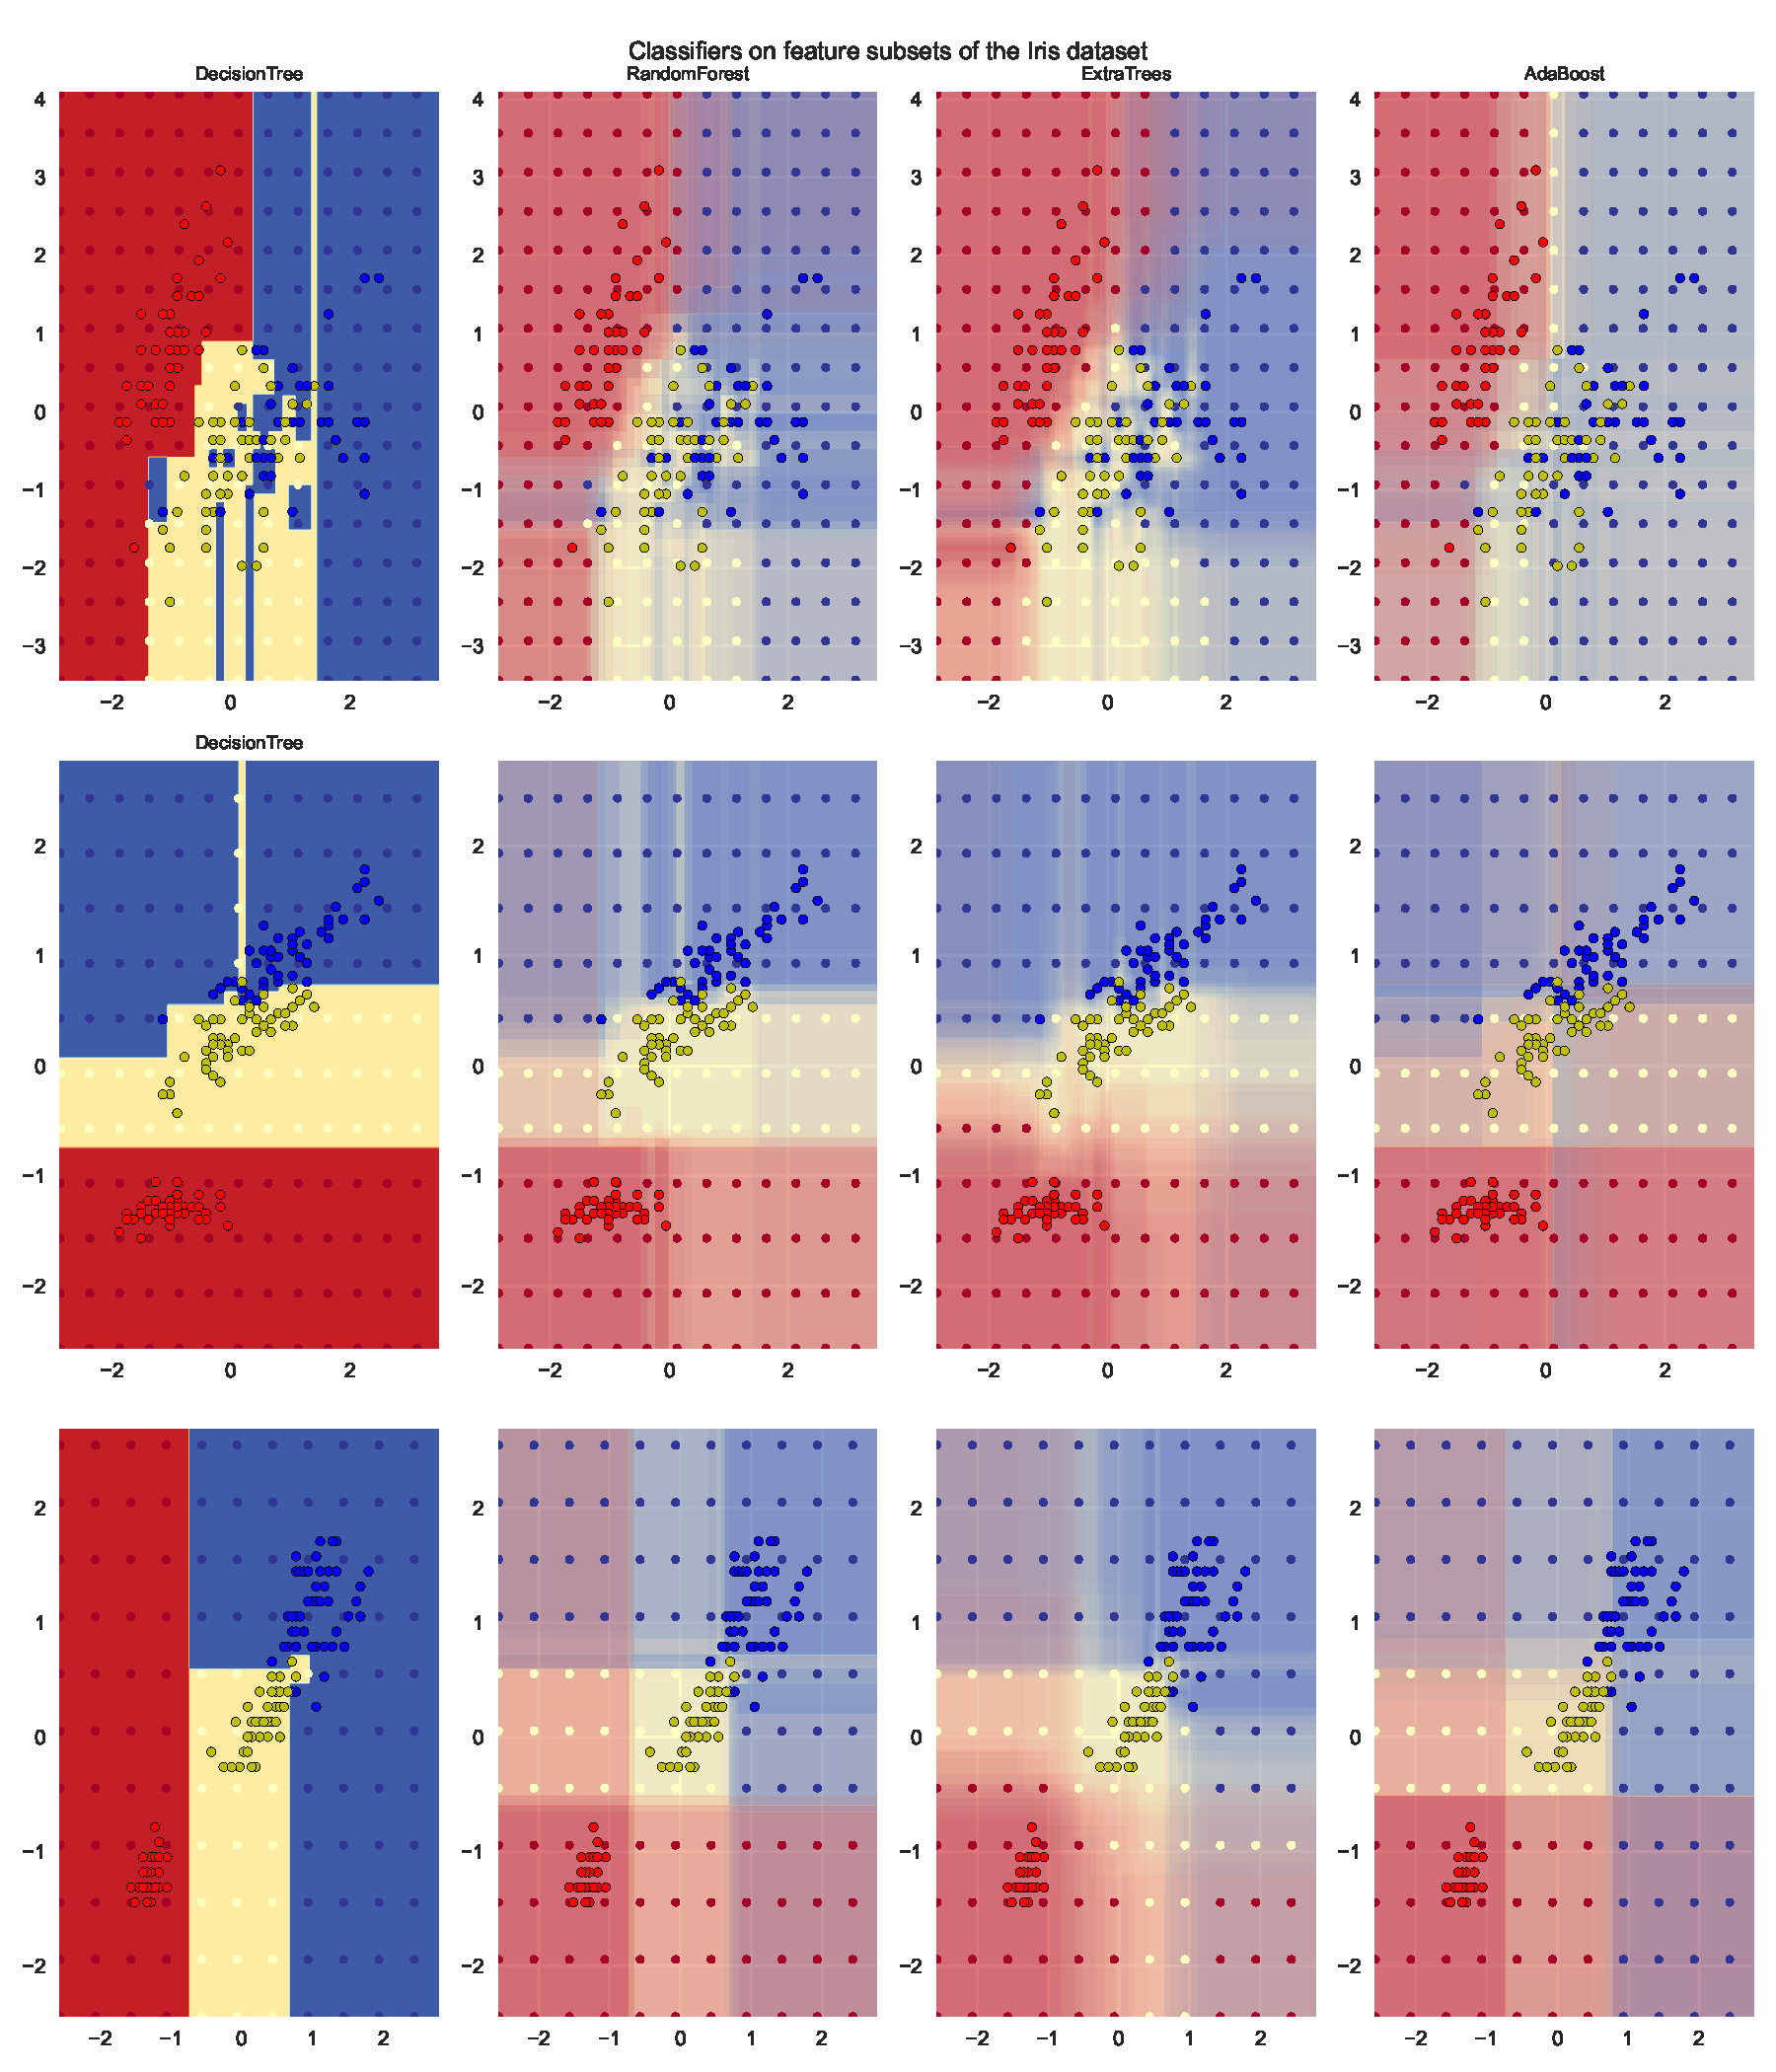
\includegraphics[width=14cm]{codeimage/code2}
	\caption{code2}
	\label{code2}
\end{figure}

\begin{PythonCode}\label{例3}
	\begin{Verbatim}[commandchars=\\\{\}]
\PY{c+c1}{\PYZsh{} 导入操作系统库}
\PY{k+kn}{import} \PY{n+nn}{os}
\PY{c+c1}{\PYZsh{} 更改工作目录}
\PY{n}{os}\PY{o}{.}\PY{n}{chdir}\PY{p}{(}\PY{l+s+sa}{r}\PY{l+s+s2}{\PYZdq{}}\PY{l+s+s2}{D:}\PY{l+s+s2}{\PYZbs{}}\PY{l+s+s2}{softwares}\PY{l+s+s2}{\PYZbs{}}\PY{l+s+s2}{applied statistics}\PY{l+s+s2}{\PYZbs{}}\PY{l+s+s2}{pythoncodelearning}\PY{l+s+s2}{\PYZbs{}}\PY{l+s+s2}{chap6}\PY{l+s+s2}{\PYZbs{}}\PY{l+s+s2}{sourcecode}\PY{l+s+s2}{\PYZdq{}}\PY{p}{)}
\PY{c+c1}{\PYZsh{} 导入基础计算库}
\PY{k+kn}{import} \PY{n+nn}{numpy} \PY{k}{as} \PY{n+nn}{np}
\PY{c+c1}{\PYZsh{} 导入绘图库}
\PY{k+kn}{import} \PY{n+nn}{matplotlib}\PY{n+nn}{.}\PY{n+nn}{pyplot} \PY{k}{as} \PY{n+nn}{plt}
\PY{c+c1}{\PYZsh{} 导入数据集工具}
\PY{k+kn}{from} \PY{n+nn}{sklearn}\PY{n+nn}{.}\PY{n+nn}{datasets} \PY{k+kn}{import} \PY{n}{load\PYZus{}diabetes}
\PY{c+c1}{\PYZsh{} 导入集成模型}
\PY{k+kn}{from} \PY{n+nn}{sklearn}\PY{n+nn}{.}\PY{n+nn}{ensemble} \PY{k+kn}{import} \PY{n}{GradientBoostingRegressor}
\PY{c+c1}{\PYZsh{} 导入均方误差工具}
\PY{k+kn}{from} \PY{n+nn}{sklearn}\PY{n+nn}{.}\PY{n+nn}{metrics} \PY{k+kn}{import} \PY{n}{mean\PYZus{}squared\PYZus{}error}
\PY{c+c1}{\PYZsh{} 导入数据集划分工具}
\PY{k+kn}{from} \PY{n+nn}{sklearn}\PY{n+nn}{.}\PY{n+nn}{model\PYZus{}selection} \PY{k+kn}{import} \PY{n}{train\PYZus{}test\PYZus{}split}
\PY{c+c1}{\PYZsh{} 导入绘图库中的字体管理包}
\PY{k+kn}{from} \PY{n+nn}{matplotlib} \PY{k+kn}{import} \PY{n}{font\PYZus{}manager}
\PY{c+c1}{\PYZsh{} 实现中文字符正常显示}
\PY{n}{font} \PY{o}{=} \PY{n}{font\PYZus{}manager}\PY{o}{.}\PY{n}{FontProperties}\PY{p}{(}\PY{n}{fname}\PY{o}{=}\PY{l+s+sa}{r}\PY{l+s+s2}{\PYZdq{}}\PY{l+s+s2}{C:}\PY{l+s+s2}{\PYZbs{}}\PY{l+s+s2}{Windows}\PY{l+s+s2}{\PYZbs{}}\PY{l+s+s2}{Fonts}\PY{l+s+s2}{\PYZbs{}}\PY{l+s+s2}{SimKai.ttf}\PY{l+s+s2}{\PYZdq{}}\PY{p}{)}
\PY{c+c1}{\PYZsh{} 使用seaborn风格绘图}
\PY{n}{plt}\PY{o}{.}\PY{n}{style}\PY{o}{.}\PY{n}{use}\PY{p}{(}\PY{l+s+s2}{\PYZdq{}}\PY{l+s+s2}{seaborn\PYZhy{}v0\PYZus{}8}\PY{l+s+s2}{\PYZdq{}}\PY{p}{)}
\PY{c+c1}{\PYZsh{} 加载数据集}
\PY{n}{diabetes} \PY{o}{=} \PY{n}{load\PYZus{}diabetes}\PY{p}{(}\PY{p}{)}
\PY{n}{X}\PY{p}{,} \PY{n}{y} \PY{o}{=} \PY{n}{diabetes}\PY{o}{.}\PY{n}{data}\PY{p}{,} \PY{n}{diabetes}\PY{o}{.}\PY{n}{target}
\PY{c+c1}{\PYZsh{} 划分数据集}
\PY{n}{X\PYZus{}train}\PY{p}{,} \PY{n}{X\PYZus{}test}\PY{p}{,} \PY{n}{y\PYZus{}train}\PY{p}{,} \PY{n}{y\PYZus{}test} \PY{o}{=} \PY{n}{train\PYZus{}test\PYZus{}split}\PY{p}{(}
    \PY{n}{X}\PY{p}{,} \PY{n}{y}\PY{p}{,} \PY{n}{test\PYZus{}size}\PY{o}{=}\PY{l+m+mf}{0.1}\PY{p}{,} \PY{n}{random\PYZus{}state}\PY{o}{=}\PY{l+m+mi}{13}
\PY{p}{)}
\PY{c+c1}{\PYZsh{} 设置一些参数}
\PY{n}{params} \PY{o}{=} \PY{p}{\PYZob{}}
    \PY{l+s+s2}{\PYZdq{}}\PY{l+s+s2}{n\PYZus{}estimators}\PY{l+s+s2}{\PYZdq{}}\PY{p}{:} \PY{l+m+mi}{500}\PY{p}{,}
    \PY{l+s+s2}{\PYZdq{}}\PY{l+s+s2}{max\PYZus{}depth}\PY{l+s+s2}{\PYZdq{}}\PY{p}{:} \PY{l+m+mi}{4}\PY{p}{,}
    \PY{l+s+s2}{\PYZdq{}}\PY{l+s+s2}{min\PYZus{}samples\PYZus{}split}\PY{l+s+s2}{\PYZdq{}}\PY{p}{:} \PY{l+m+mi}{5}\PY{p}{,}
    \PY{l+s+s2}{\PYZdq{}}\PY{l+s+s2}{learning\PYZus{}rate}\PY{l+s+s2}{\PYZdq{}}\PY{p}{:} \PY{l+m+mf}{0.01}\PY{p}{,}
    \PY{l+s+s2}{\PYZdq{}}\PY{l+s+s2}{loss}\PY{l+s+s2}{\PYZdq{}}\PY{p}{:} \PY{l+s+s2}{\PYZdq{}}\PY{l+s+s2}{squared\PYZus{}error}\PY{l+s+s2}{\PYZdq{}}\PY{p}{,}
\PY{p}{\PYZcb{}}
\PY{c+c1}{\PYZsh{} 构建模型}
\PY{n}{reg} \PY{o}{=} \PY{n}{GradientBoostingRegressor}\PY{p}{(}\PY{o}{*}\PY{o}{*}\PY{n}{params}\PY{p}{)}
\PY{c+c1}{\PYZsh{} 模型拟合}
\PY{n}{reg}\PY{o}{.}\PY{n}{fit}\PY{p}{(}\PY{n}{X\PYZus{}train}\PY{p}{,} \PY{n}{y\PYZus{}train}\PY{p}{)}
\PY{c+c1}{\PYZsh{} 预测}
\PY{n}{y\PYZus{}pred} \PY{o}{=} \PY{n}{reg}\PY{o}{.}\PY{n}{predict}\PY{p}{(}\PY{n}{X\PYZus{}test}\PY{p}{)}
\PY{c+c1}{\PYZsh{} 均方误差}
\PY{n}{mse} \PY{o}{=} \PY{n}{mean\PYZus{}squared\PYZus{}error}\PY{p}{(}\PY{n}{y\PYZus{}test}\PY{p}{,} \PY{n}{y\PYZus{}pred}\PY{p}{)}
\PY{n+nb}{print}\PY{p}{(}\PY{l+s+s2}{\PYZdq{}}\PY{l+s+s2}{The mean squared error (MSE) on test set: }\PY{l+s+si}{\PYZob{}:.4f\PYZcb{}}\PY{l+s+s2}{\PYZdq{}}\PY{o}{.}\PY{n}{format}\PY{p}{(}\PY{n}{mse}\PY{p}{)}\PY{p}{)}
\PY{c+c1}{\PYZsh{} 初始化测试集上的mse}
\PY{n}{test\PYZus{}score} \PY{o}{=} \PY{n}{np}\PY{o}{.}\PY{n}{zeros}\PY{p}{(}\PY{p}{(}\PY{n}{params}\PY{p}{[}\PY{l+s+s2}{\PYZdq{}}\PY{l+s+s2}{n\PYZus{}estimators}\PY{l+s+s2}{\PYZdq{}}\PY{p}{]}\PY{p}{,}\PY{p}{)}\PY{p}{,} \PY{n}{dtype}\PY{o}{=}\PY{n}{np}\PY{o}{.}\PY{n}{float64}\PY{p}{)}
\PY{c+c1}{\PYZsh{} 阶段性预测X\PYZus{}test}
\PY{k}{for} \PY{n}{i}\PY{p}{,} \PY{n}{y\PYZus{}pred} \PY{o+ow}{in} \PY{n+nb}{enumerate}\PY{p}{(}\PY{n}{reg}\PY{o}{.}\PY{n}{staged\PYZus{}predict}\PY{p}{(}\PY{n}{X\PYZus{}test}\PY{p}{)}\PY{p}{)}\PY{p}{:}
    \PY{c+c1}{\PYZsh{} 得到回归的mse}
    \PY{n}{test\PYZus{}score}\PY{p}{[}\PY{n}{i}\PY{p}{]} \PY{o}{=} \PY{n}{mean\PYZus{}squared\PYZus{}error}\PY{p}{(}\PY{n}{y\PYZus{}test}\PY{p}{,} \PY{n}{y\PYZus{}pred}\PY{p}{)}

\PY{n}{fig}\PY{p}{,} \PY{n}{ax} \PY{o}{=} \PY{n}{plt}\PY{o}{.}\PY{n}{subplots}\PY{p}{(}\PY{n}{figsize}\PY{o}{=}\PY{p}{(}\PY{l+m+mi}{6}\PY{p}{,} \PY{l+m+mi}{6}\PY{p}{)}\PY{p}{,} \PY{n}{tight\PYZus{}layout}\PY{o}{=}\PY{k+kc}{True}\PY{p}{)}
\PY{n}{ax}\PY{o}{.}\PY{n}{set\PYZus{}title}\PY{p}{(}\PY{l+s+s2}{\PYZdq{}}\PY{l+s+s2}{Deviance}\PY{l+s+s2}{\PYZdq{}}\PY{p}{)}
\PY{n}{ax}\PY{o}{.}\PY{n}{plot}\PY{p}{(}
    \PY{n}{np}\PY{o}{.}\PY{n}{arange}\PY{p}{(}\PY{n}{params}\PY{p}{[}\PY{l+s+s2}{\PYZdq{}}\PY{l+s+s2}{n\PYZus{}estimators}\PY{l+s+s2}{\PYZdq{}}\PY{p}{]}\PY{p}{)} \PY{o}{+} \PY{l+m+mi}{1}\PY{p}{,}
    \PY{n}{reg}\PY{o}{.}\PY{n}{train\PYZus{}score\PYZus{}}\PY{p}{,}
    \PY{l+s+s2}{\PYZdq{}}\PY{l+s+s2}{b\PYZhy{}}\PY{l+s+s2}{\PYZdq{}}\PY{p}{,}
    \PY{n}{label}\PY{o}{=}\PY{l+s+s2}{\PYZdq{}}\PY{l+s+s2}{Training Set Deviance}\PY{l+s+s2}{\PYZdq{}}\PY{p}{,}
\PY{p}{)}
\PY{n}{ax}\PY{o}{.}\PY{n}{plot}\PY{p}{(}
    \PY{n}{np}\PY{o}{.}\PY{n}{arange}\PY{p}{(}\PY{n}{params}\PY{p}{[}\PY{l+s+s2}{\PYZdq{}}\PY{l+s+s2}{n\PYZus{}estimators}\PY{l+s+s2}{\PYZdq{}}\PY{p}{]}\PY{p}{)} \PY{o}{+} \PY{l+m+mi}{1}\PY{p}{,} 
    \PY{n}{test\PYZus{}score}\PY{p}{,} \PY{l+s+s2}{\PYZdq{}}\PY{l+s+s2}{r\PYZhy{}}\PY{l+s+s2}{\PYZdq{}}\PY{p}{,} \PY{n}{label}\PY{o}{=}\PY{l+s+s2}{\PYZdq{}}\PY{l+s+s2}{Test Set Deviance}\PY{l+s+s2}{\PYZdq{}}
\PY{p}{)}
\PY{n}{ax}\PY{o}{.}\PY{n}{legend}\PY{p}{(}\PY{n}{loc}\PY{o}{=}\PY{l+s+s2}{\PYZdq{}}\PY{l+s+s2}{upper right}\PY{l+s+s2}{\PYZdq{}}\PY{p}{)}
\PY{n}{ax}\PY{o}{.}\PY{n}{set\PYZus{}xlabel}\PY{p}{(}\PY{l+s+s2}{\PYZdq{}}\PY{l+s+s2}{Boosting Iterations}\PY{l+s+s2}{\PYZdq{}}\PY{p}{)}
\PY{n}{ax}\PY{o}{.}\PY{n}{set\PYZus{}ylabel}\PY{p}{(}\PY{l+s+s2}{\PYZdq{}}\PY{l+s+s2}{Deviance}\PY{l+s+s2}{\PYZdq{}}\PY{p}{)}
\PY{n}{plt}\PY{o}{.}\PY{n}{show}\PY{p}{(}\PY{p}{)}
\PY{n}{fig}\PY{o}{.}\PY{n}{savefig}\PY{p}{(}\PY{l+s+s2}{\PYZdq{}}\PY{l+s+s2}{../codeimage/code3.pdf}\PY{l+s+s2}{\PYZdq{}}\PY{p}{)}
\end{Verbatim}

\begin{Verbatim}[commandchars=\\\{\}]
The mean squared error (MSE) on test set: 3041.0505
\end{Verbatim}
\end{PythonCode}

\begin{figure}[htbp]
	\centering
	\includegraphics[width=14cm]{codeimage/code3}
	\caption{code3}
	\label{code3}
\end{figure}

\begin{PythonCode}\label{例4}
	\begin{Verbatim}[commandchars=\\\{\}]
\PY{c+c1}{\PYZsh{} 导入操作系统库}
\PY{k+kn}{import} \PY{n+nn}{os}
\PY{c+c1}{\PYZsh{} 更改工作目录}
\PY{n}{os}\PY{o}{.}\PY{n}{chdir}\PY{p}{(}\PY{l+s+sa}{r}\PY{l+s+s2}{\PYZdq{}}\PY{l+s+s2}{D:}\PY{l+s+s2}{\PYZbs{}}\PY{l+s+s2}{softwares}\PY{l+s+s2}{\PYZbs{}}\PY{l+s+s2}{applied statistics}\PY{l+s+s2}{\PYZbs{}}\PY{l+s+s2}{pythoncodelearning}\PY{l+s+s2}{\PYZbs{}}\PY{l+s+s2}{chap5}\PY{l+s+s2}{\PYZbs{}}\PY{l+s+s2}{sourcecode}\PY{l+s+s2}{\PYZdq{}}\PY{p}{)}
\PY{c+c1}{\PYZsh{} 导入绘图库}
\PY{k+kn}{import} \PY{n+nn}{matplotlib}\PY{n+nn}{.}\PY{n+nn}{pyplot} \PY{k}{as} \PY{n+nn}{plt}
\PY{c+c1}{\PYZsh{} 导入数据集划分工具}
\PY{k+kn}{from} \PY{n+nn}{sklearn}\PY{n+nn}{.}\PY{n+nn}{model\PYZus{}selection} \PY{k+kn}{import} \PY{n}{train\PYZus{}test\PYZus{}split}
\PY{c+c1}{\PYZsh{} 导入数据集工具}
\PY{k+kn}{from} \PY{n+nn}{sklearn}\PY{n+nn}{.}\PY{n+nn}{datasets} \PY{k+kn}{import} \PY{n}{load\PYZus{}breast\PYZus{}cancer}
\PY{c+c1}{\PYZsh{} 导入分类树}
\PY{k+kn}{from} \PY{n+nn}{sklearn}\PY{n+nn}{.}\PY{n+nn}{tree} \PY{k+kn}{import} \PY{n}{DecisionTreeClassifier}
\PY{c+c1}{\PYZsh{} 导入绘图库中的字体管理包}
\PY{k+kn}{from} \PY{n+nn}{matplotlib} \PY{k+kn}{import} \PY{n}{font\PYZus{}manager}
\PY{c+c1}{\PYZsh{} 实现中文字符正常显示}
\PY{n}{font} \PY{o}{=} \PY{n}{font\PYZus{}manager}\PY{o}{.}\PY{n}{FontProperties}\PY{p}{(}\PY{n}{fname}\PY{o}{=}\PY{l+s+sa}{r}\PY{l+s+s2}{\PYZdq{}}\PY{l+s+s2}{C:}\PY{l+s+s2}{\PYZbs{}}\PY{l+s+s2}{Windows}\PY{l+s+s2}{\PYZbs{}}\PY{l+s+s2}{Fonts}\PY{l+s+s2}{\PYZbs{}}\PY{l+s+s2}{SimKai.ttf}\PY{l+s+s2}{\PYZdq{}}\PY{p}{)}
\PY{c+c1}{\PYZsh{} 使用seaborn风格绘图}
\PY{n}{plt}\PY{o}{.}\PY{n}{style}\PY{o}{.}\PY{n}{use}\PY{p}{(}\PY{l+s+s2}{\PYZdq{}}\PY{l+s+s2}{seaborn\PYZhy{}v0\PYZus{}8}\PY{l+s+s2}{\PYZdq{}}\PY{p}{)}
\PY{c+c1}{\PYZsh{} 获取数据}
\PY{n}{X}\PY{p}{,} \PY{n}{y} \PY{o}{=} \PY{n}{load\PYZus{}breast\PYZus{}cancer}\PY{p}{(}\PY{n}{return\PYZus{}X\PYZus{}y}\PY{o}{=}\PY{k+kc}{True}\PY{p}{)}
\PY{c+c1}{\PYZsh{} 数据集划分}
\PY{n}{X\PYZus{}train}\PY{p}{,} \PY{n}{X\PYZus{}test}\PY{p}{,} \PY{n}{y\PYZus{}train}\PY{p}{,} \PY{n}{y\PYZus{}test} \PY{o}{=} \PY{n}{train\PYZus{}test\PYZus{}split}\PY{p}{(}
    \PY{n}{X}\PY{p}{,} \PY{n}{y}\PY{p}{,} \PY{n}{random\PYZus{}state}\PY{o}{=}\PY{l+m+mi}{0}
\PY{p}{)}
\PY{c+c1}{\PYZsh{} 构建决策树}
\PY{n}{clf} \PY{o}{=} \PY{n}{DecisionTreeClassifier}\PY{p}{(}\PY{n}{random\PYZus{}state}\PY{o}{=}\PY{l+m+mi}{0}\PY{p}{)}
\PY{c+c1}{\PYZsh{} 代价复杂度路径}
\PY{n}{path} \PY{o}{=} \PY{n}{clf}\PY{o}{.}\PY{n}{cost\PYZus{}complexity\PYZus{}pruning\PYZus{}path}\PY{p}{(}\PY{n}{X\PYZus{}train}\PY{p}{,} \PY{n}{y\PYZus{}train}\PY{p}{)}
\PY{c+c1}{\PYZsh{} cp}
\PY{n}{ccp\PYZus{}alphas}\PY{p}{,} \PY{n}{impurities} \PY{o}{=} \PY{n}{path}\PY{o}{.}\PY{n}{ccp\PYZus{}alphas}\PY{p}{,} \PY{n}{path}\PY{o}{.}\PY{n}{impurities}
\PY{c+c1}{\PYZsh{} 绘图}
\PY{n}{fig}\PY{p}{,} \PY{n}{ax} \PY{o}{=} \PY{n}{plt}\PY{o}{.}\PY{n}{subplots}\PY{p}{(}\PY{n}{figsize}\PY{o}{=}\PY{p}{(}\PY{l+m+mi}{6}\PY{p}{,}\PY{l+m+mi}{6}\PY{p}{)}\PY{p}{)}
\PY{n}{ax}\PY{o}{.}\PY{n}{plot}\PY{p}{(}\PY{n}{ccp\PYZus{}alphas}\PY{p}{[}\PY{p}{:}\PY{o}{\PYZhy{}}\PY{l+m+mi}{1}\PY{p}{]}\PY{p}{,} \PY{n}{impurities}\PY{p}{[}\PY{p}{:}\PY{o}{\PYZhy{}}\PY{l+m+mi}{1}\PY{p}{]}\PY{p}{,} \PY{n}{marker}\PY{o}{=}\PY{l+s+s2}{\PYZdq{}}\PY{l+s+s2}{o}\PY{l+s+s2}{\PYZdq{}}\PY{p}{,} \PY{n}{drawstyle}\PY{o}{=}\PY{l+s+s2}{\PYZdq{}}\PY{l+s+s2}{steps\PYZhy{}post}\PY{l+s+s2}{\PYZdq{}}\PY{p}{)}
\PY{n}{ax}\PY{o}{.}\PY{n}{set\PYZus{}xlabel}\PY{p}{(}\PY{l+s+s2}{\PYZdq{}}\PY{l+s+s2}{effective alpha}\PY{l+s+s2}{\PYZdq{}}\PY{p}{)}
\PY{n}{ax}\PY{o}{.}\PY{n}{set\PYZus{}ylabel}\PY{p}{(}\PY{l+s+s2}{\PYZdq{}}\PY{l+s+s2}{total impurity of leaves}\PY{l+s+s2}{\PYZdq{}}\PY{p}{)}
\PY{n}{ax}\PY{o}{.}\PY{n}{set\PYZus{}title}\PY{p}{(}\PY{l+s+s2}{\PYZdq{}}\PY{l+s+s2}{Total Impurity vs effective alpha for training set}\PY{l+s+s2}{\PYZdq{}}\PY{p}{)}
\PY{n}{plt}\PY{o}{.}\PY{n}{show}\PY{p}{(}\PY{p}{)}
\PY{n}{fig}\PY{o}{.}\PY{n}{savefig}\PY{p}{(}\PY{l+s+s2}{\PYZdq{}}\PY{l+s+s2}{../codeimage/code4.pdf}\PY{l+s+s2}{\PYZdq{}}\PY{p}{)}
\PY{c+c1}{\PYZsh{} 不同的alpha下构建决策树}
\PY{n}{clfs} \PY{o}{=} \PY{p}{[}\PY{p}{]}
\PY{k}{for} \PY{n}{ccp\PYZus{}alpha} \PY{o+ow}{in} \PY{n}{ccp\PYZus{}alphas}\PY{p}{:}
    \PY{c+c1}{\PYZsh{} 构建模型}
    \PY{n}{clf} \PY{o}{=} \PY{n}{DecisionTreeClassifier}\PY{p}{(}
        \PY{n}{random\PYZus{}state}\PY{o}{=}\PY{l+m+mi}{0}\PY{p}{,} \PY{n}{ccp\PYZus{}alpha}\PY{o}{=}\PY{n}{ccp\PYZus{}alpha}
    \PY{p}{)}
    \PY{c+c1}{\PYZsh{} 模拟拟合}
    \PY{n}{clf}\PY{o}{.}\PY{n}{fit}\PY{p}{(}\PY{n}{X\PYZus{}train}\PY{p}{,} \PY{n}{y\PYZus{}train}\PY{p}{)}
    \PY{c+c1}{\PYZsh{} 加入到列表中}
    \PY{n}{clfs}\PY{o}{.}\PY{n}{append}\PY{p}{(}\PY{n}{clf}\PY{p}{)}
\PY{n+nb}{print}\PY{p}{(}
    \PY{l+s+s2}{\PYZdq{}}\PY{l+s+s2}{Number of nodes in the last tree is: }\PY{l+s+si}{\PYZob{}\PYZcb{}}\PY{l+s+s2}{ with ccp\PYZus{}alpha: }\PY{l+s+si}{\PYZob{}\PYZcb{}}\PY{l+s+s2}{\PYZdq{}}\PY{o}{.}\PY{n}{format}\PY{p}{(}
        \PY{n}{clfs}\PY{p}{[}\PY{o}{\PYZhy{}}\PY{l+m+mi}{1}\PY{p}{]}\PY{o}{.}\PY{n}{tree\PYZus{}}\PY{o}{.}\PY{n}{node\PYZus{}count}\PY{p}{,} \PY{n}{ccp\PYZus{}alphas}\PY{p}{[}\PY{o}{\PYZhy{}}\PY{l+m+mi}{1}\PY{p}{]}
    \PY{p}{)}
\PY{p}{)}
\PY{c+c1}{\PYZsh{} 去掉最后一个}
\PY{n}{clfs} \PY{o}{=} \PY{n}{clfs}\PY{p}{[}\PY{p}{:}\PY{o}{\PYZhy{}}\PY{l+m+mi}{1}\PY{p}{]}
\PY{n}{ccp\PYZus{}alphas} \PY{o}{=} \PY{n}{ccp\PYZus{}alphas}\PY{p}{[}\PY{p}{:}\PY{o}{\PYZhy{}}\PY{l+m+mi}{1}\PY{p}{]}
\PY{c+c1}{\PYZsh{} 节点数量}
\PY{n}{node\PYZus{}counts} \PY{o}{=} \PY{p}{[}\PY{n}{clf}\PY{o}{.}\PY{n}{tree\PYZus{}}\PY{o}{.}\PY{n}{node\PYZus{}count} \PY{k}{for} \PY{n}{clf} \PY{o+ow}{in} \PY{n}{clfs}\PY{p}{]}
\PY{c+c1}{\PYZsh{} 深度}
\PY{n}{depth} \PY{o}{=} \PY{p}{[}\PY{n}{clf}\PY{o}{.}\PY{n}{tree\PYZus{}}\PY{o}{.}\PY{n}{max\PYZus{}depth} \PY{k}{for} \PY{n}{clf} \PY{o+ow}{in} \PY{n}{clfs}\PY{p}{]}
\PY{n}{fig}\PY{p}{,} \PY{n}{ax} \PY{o}{=} \PY{n}{plt}\PY{o}{.}\PY{n}{subplots}\PY{p}{(}\PY{l+m+mi}{2}\PY{p}{,} \PY{l+m+mi}{1}\PY{p}{,} \PY{n}{figsize}\PY{o}{=}\PY{p}{(}\PY{l+m+mi}{6}\PY{p}{,}\PY{l+m+mi}{6}\PY{p}{)}\PY{p}{,} \PY{n}{tight\PYZus{}layout}\PY{o}{=}\PY{k+kc}{True}\PY{p}{)}
\PY{n}{ax}\PY{p}{[}\PY{l+m+mi}{0}\PY{p}{]}\PY{o}{.}\PY{n}{plot}\PY{p}{(}\PY{n}{ccp\PYZus{}alphas}\PY{p}{,} \PY{n}{node\PYZus{}counts}\PY{p}{,} \PY{n}{marker}\PY{o}{=}\PY{l+s+s2}{\PYZdq{}}\PY{l+s+s2}{o}\PY{l+s+s2}{\PYZdq{}}\PY{p}{,} \PY{n}{drawstyle}\PY{o}{=}\PY{l+s+s2}{\PYZdq{}}\PY{l+s+s2}{steps\PYZhy{}post}\PY{l+s+s2}{\PYZdq{}}\PY{p}{)}
\PY{n}{ax}\PY{p}{[}\PY{l+m+mi}{0}\PY{p}{]}\PY{o}{.}\PY{n}{set\PYZus{}xlabel}\PY{p}{(}\PY{l+s+s2}{\PYZdq{}}\PY{l+s+s2}{alpha}\PY{l+s+s2}{\PYZdq{}}\PY{p}{)}
\PY{n}{ax}\PY{p}{[}\PY{l+m+mi}{0}\PY{p}{]}\PY{o}{.}\PY{n}{set\PYZus{}ylabel}\PY{p}{(}\PY{l+s+s2}{\PYZdq{}}\PY{l+s+s2}{number of nodes}\PY{l+s+s2}{\PYZdq{}}\PY{p}{)}
\PY{n}{ax}\PY{p}{[}\PY{l+m+mi}{0}\PY{p}{]}\PY{o}{.}\PY{n}{set\PYZus{}title}\PY{p}{(}\PY{l+s+s2}{\PYZdq{}}\PY{l+s+s2}{Number of nodes vs alpha}\PY{l+s+s2}{\PYZdq{}}\PY{p}{)}
\PY{n}{ax}\PY{p}{[}\PY{l+m+mi}{1}\PY{p}{]}\PY{o}{.}\PY{n}{plot}\PY{p}{(}\PY{n}{ccp\PYZus{}alphas}\PY{p}{,} \PY{n}{depth}\PY{p}{,} \PY{n}{marker}\PY{o}{=}\PY{l+s+s2}{\PYZdq{}}\PY{l+s+s2}{o}\PY{l+s+s2}{\PYZdq{}}\PY{p}{,} \PY{n}{drawstyle}\PY{o}{=}\PY{l+s+s2}{\PYZdq{}}\PY{l+s+s2}{steps\PYZhy{}post}\PY{l+s+s2}{\PYZdq{}}\PY{p}{)}
\PY{n}{ax}\PY{p}{[}\PY{l+m+mi}{1}\PY{p}{]}\PY{o}{.}\PY{n}{set\PYZus{}xlabel}\PY{p}{(}\PY{l+s+s2}{\PYZdq{}}\PY{l+s+s2}{alpha}\PY{l+s+s2}{\PYZdq{}}\PY{p}{)}
\PY{n}{ax}\PY{p}{[}\PY{l+m+mi}{1}\PY{p}{]}\PY{o}{.}\PY{n}{set\PYZus{}ylabel}\PY{p}{(}\PY{l+s+s2}{\PYZdq{}}\PY{l+s+s2}{depth of tree}\PY{l+s+s2}{\PYZdq{}}\PY{p}{)}
\PY{n}{ax}\PY{p}{[}\PY{l+m+mi}{1}\PY{p}{]}\PY{o}{.}\PY{n}{set\PYZus{}title}\PY{p}{(}\PY{l+s+s2}{\PYZdq{}}\PY{l+s+s2}{Depth vs alpha}\PY{l+s+s2}{\PYZdq{}}\PY{p}{)}
\PY{n}{plt}\PY{o}{.}\PY{n}{show}\PY{p}{(}\PY{p}{)}
\PY{n}{fig}\PY{o}{.}\PY{n}{savefig}\PY{p}{(}\PY{l+s+s2}{\PYZdq{}}\PY{l+s+s2}{../codeimage/code5.pdf}\PY{l+s+s2}{\PYZdq{}}\PY{p}{)}
\PY{c+c1}{\PYZsh{} 预测精度和alpha的关系}
\PY{c+c1}{\PYZsh{} 训练集的准确率}
\PY{n}{train\PYZus{}scores} \PY{o}{=} \PY{p}{[}\PY{n}{clf}\PY{o}{.}\PY{n}{score}\PY{p}{(}\PY{n}{X\PYZus{}train}\PY{p}{,} \PY{n}{y\PYZus{}train}\PY{p}{)} \PY{k}{for} \PY{n}{clf} \PY{o+ow}{in} \PY{n}{clfs}\PY{p}{]}
\PY{c+c1}{\PYZsh{} 测试集的准确率}
\PY{n}{test\PYZus{}scores} \PY{o}{=} \PY{p}{[}\PY{n}{clf}\PY{o}{.}\PY{n}{score}\PY{p}{(}\PY{n}{X\PYZus{}test}\PY{p}{,} \PY{n}{y\PYZus{}test}\PY{p}{)} \PY{k}{for} \PY{n}{clf} \PY{o+ow}{in} \PY{n}{clfs}\PY{p}{]}
\PY{n}{fig}\PY{p}{,} \PY{n}{ax} \PY{o}{=} \PY{n}{plt}\PY{o}{.}\PY{n}{subplots}\PY{p}{(}\PY{n}{figsize}\PY{o}{=}\PY{p}{(}\PY{l+m+mi}{6}\PY{p}{,}\PY{l+m+mi}{6}\PY{p}{)}\PY{p}{)}
\PY{n}{ax}\PY{o}{.}\PY{n}{set\PYZus{}xlabel}\PY{p}{(}\PY{l+s+s2}{\PYZdq{}}\PY{l+s+s2}{alpha}\PY{l+s+s2}{\PYZdq{}}\PY{p}{)}
\PY{n}{ax}\PY{o}{.}\PY{n}{set\PYZus{}ylabel}\PY{p}{(}\PY{l+s+s2}{\PYZdq{}}\PY{l+s+s2}{accuracy}\PY{l+s+s2}{\PYZdq{}}\PY{p}{)}
\PY{n}{ax}\PY{o}{.}\PY{n}{set\PYZus{}title}\PY{p}{(}\PY{l+s+s2}{\PYZdq{}}\PY{l+s+s2}{Accuracy vs alpha for training and testing sets}\PY{l+s+s2}{\PYZdq{}}\PY{p}{)}
\PY{n}{ax}\PY{o}{.}\PY{n}{plot}\PY{p}{(}\PY{n}{ccp\PYZus{}alphas}\PY{p}{,} \PY{n}{train\PYZus{}scores}\PY{p}{,} \PY{n}{marker}\PY{o}{=}\PY{l+s+s2}{\PYZdq{}}\PY{l+s+s2}{o}\PY{l+s+s2}{\PYZdq{}}\PY{p}{,} \PY{n}{label}\PY{o}{=}\PY{l+s+s2}{\PYZdq{}}\PY{l+s+s2}{train}\PY{l+s+s2}{\PYZdq{}}\PY{p}{,} \PY{n}{drawstyle}\PY{o}{=}\PY{l+s+s2}{\PYZdq{}}\PY{l+s+s2}{steps\PYZhy{}post}\PY{l+s+s2}{\PYZdq{}}\PY{p}{)}
\PY{n}{ax}\PY{o}{.}\PY{n}{plot}\PY{p}{(}\PY{n}{ccp\PYZus{}alphas}\PY{p}{,} \PY{n}{test\PYZus{}scores}\PY{p}{,} \PY{n}{marker}\PY{o}{=}\PY{l+s+s2}{\PYZdq{}}\PY{l+s+s2}{o}\PY{l+s+s2}{\PYZdq{}}\PY{p}{,} \PY{n}{label}\PY{o}{=}\PY{l+s+s2}{\PYZdq{}}\PY{l+s+s2}{test}\PY{l+s+s2}{\PYZdq{}}\PY{p}{,} \PY{n}{drawstyle}\PY{o}{=}\PY{l+s+s2}{\PYZdq{}}\PY{l+s+s2}{steps\PYZhy{}post}\PY{l+s+s2}{\PYZdq{}}\PY{p}{)}
\PY{n}{ax}\PY{o}{.}\PY{n}{legend}\PY{p}{(}\PY{p}{)}
\PY{n}{plt}\PY{o}{.}\PY{n}{show}\PY{p}{(}\PY{p}{)}
\PY{n}{fig}\PY{o}{.}\PY{n}{savefig}\PY{p}{(}\PY{l+s+s2}{\PYZdq{}}\PY{l+s+s2}{../codeimage/code6.pdf}\PY{l+s+s2}{\PYZdq{}}\PY{p}{)}
\end{Verbatim}
    
\begin{Verbatim}[commandchars=\\\{\}]
Number of nodes in the last tree is: 1 with ccp\_alpha: 0.3272984419327777
\end{Verbatim}
\end{PythonCode}

\begin{figure}[htbp]
	\centering
	\includegraphics[width=14cm]{codeimage/code4}
	\caption{code4}
	\label{code4}
\end{figure}

\begin{PythonCode}\label{例5}
	\begin{Verbatim}[commandchars=\\\{\}]
\PY{c+c1}{\PYZsh{} 导入操作系统库}
\PY{k+kn}{import} \PY{n+nn}{os}
\PY{c+c1}{\PYZsh{} 更改工作目录}
\PY{n}{os}\PY{o}{.}\PY{n}{chdir}\PY{p}{(}\PY{l+s+sa}{r}\PY{l+s+s2}{\PYZdq{}}\PY{l+s+s2}{D:}\PY{l+s+s2}{\PYZbs{}}\PY{l+s+s2}{softwares}\PY{l+s+s2}{\PYZbs{}}\PY{l+s+s2}{applied statistics}\PY{l+s+s2}{\PYZbs{}}\PY{l+s+s2}{pythoncodelearning}\PY{l+s+s2}{\PYZbs{}}\PY{l+s+s2}{chap6}\PY{l+s+s2}{\PYZbs{}}\PY{l+s+s2}{sourcecode}\PY{l+s+s2}{\PYZdq{}}\PY{p}{)}
\PY{c+c1}{\PYZsh{} 导入绘图库}
\PY{k+kn}{import} \PY{n+nn}{matplotlib}\PY{n+nn}{.}\PY{n+nn}{pyplot} \PY{k}{as} \PY{n+nn}{plt}
\PY{c+c1}{\PYZsh{} 导入数据集}
\PY{k+kn}{from} \PY{n+nn}{sklearn}\PY{n+nn}{.}\PY{n+nn}{datasets} \PY{k+kn}{import} \PY{n}{load\PYZus{}iris}
\PY{c+c1}{\PYZsh{} 导入决策树分类}
\PY{k+kn}{from} \PY{n+nn}{sklearn}\PY{n+nn}{.}\PY{n+nn}{tree} \PY{k+kn}{import} \PY{n}{DecisionTreeClassifier}
\PY{c+c1}{\PYZsh{} 导入KNN分类}
\PY{k+kn}{from} \PY{n+nn}{sklearn}\PY{n+nn}{.}\PY{n+nn}{neighbors} \PY{k+kn}{import} \PY{n}{KNeighborsClassifier}
\PY{c+c1}{\PYZsh{} 导入SVC}
\PY{k+kn}{from} \PY{n+nn}{sklearn}\PY{n+nn}{.}\PY{n+nn}{svm} \PY{k+kn}{import} \PY{n}{SVC}
\PY{c+c1}{\PYZsh{} 导入投票投票分类器}
\PY{k+kn}{from} \PY{n+nn}{sklearn}\PY{n+nn}{.}\PY{n+nn}{ensemble} \PY{k+kn}{import} \PY{n}{VotingClassifier}
\PY{c+c1}{\PYZsh{} 导入决策边界显示}
\PY{k+kn}{from} \PY{n+nn}{sklearn}\PY{n+nn}{.}\PY{n+nn}{inspection} \PY{k+kn}{import} \PY{n}{DecisionBoundaryDisplay}
\PY{c+c1}{\PYZsh{} 导入绘图库中的字体管理包}
\PY{k+kn}{from} \PY{n+nn}{matplotlib} \PY{k+kn}{import} \PY{n}{font\PYZus{}manager}
\PY{c+c1}{\PYZsh{} 导入product工具}
\PY{k+kn}{from} \PY{n+nn}{itertools} \PY{k+kn}{import} \PY{n}{product}
\PY{c+c1}{\PYZsh{} 实现中文字符正常显示}
\PY{n}{font} \PY{o}{=} \PY{n}{font\PYZus{}manager}\PY{o}{.}\PY{n}{FontProperties}\PY{p}{(}\PY{n}{fname}\PY{o}{=}\PY{l+s+sa}{r}\PY{l+s+s2}{\PYZdq{}}\PY{l+s+s2}{C:}\PY{l+s+s2}{\PYZbs{}}\PY{l+s+s2}{Windows}\PY{l+s+s2}{\PYZbs{}}\PY{l+s+s2}{Fonts}\PY{l+s+s2}{\PYZbs{}}\PY{l+s+s2}{SimKai.ttf}\PY{l+s+s2}{\PYZdq{}}\PY{p}{)}
\PY{c+c1}{\PYZsh{} 使用seaborn风格绘图}
\PY{n}{plt}\PY{o}{.}\PY{n}{style}\PY{o}{.}\PY{n}{use}\PY{p}{(}\PY{l+s+s2}{\PYZdq{}}\PY{l+s+s2}{seaborn\PYZhy{}v0\PYZus{}8}\PY{l+s+s2}{\PYZdq{}}\PY{p}{)}
\PY{c+c1}{\PYZsh{} 加载数据集}
\PY{n}{iris} \PY{o}{=} \PY{n}{load\PYZus{}iris}\PY{p}{(}\PY{p}{)}
\PY{c+c1}{\PYZsh{} X, Y}
\PY{n}{X} \PY{o}{=} \PY{n}{iris}\PY{o}{.}\PY{n}{data}\PY{p}{[}\PY{p}{:}\PY{p}{,} \PY{p}{[}\PY{l+m+mi}{0}\PY{p}{,} \PY{l+m+mi}{2}\PY{p}{]}\PY{p}{]}
\PY{n}{y} \PY{o}{=} \PY{n}{iris}\PY{o}{.}\PY{n}{target}
\PY{c+c1}{\PYZsh{} 决策树}
\PY{n}{clf1} \PY{o}{=} \PY{n}{DecisionTreeClassifier}\PY{p}{(}\PY{n}{max\PYZus{}depth}\PY{o}{=}\PY{l+m+mi}{4}\PY{p}{)}
\PY{c+c1}{\PYZsh{} KNN}
\PY{n}{clf2} \PY{o}{=} \PY{n}{KNeighborsClassifier}\PY{p}{(}\PY{n}{n\PYZus{}neighbors}\PY{o}{=}\PY{l+m+mi}{7}\PY{p}{)}
\PY{c+c1}{\PYZsh{} SVC}
\PY{n}{clf3} \PY{o}{=} \PY{n}{SVC}\PY{p}{(}\PY{n}{gamma}\PY{o}{=}\PY{l+m+mf}{0.1}\PY{p}{,} \PY{n}{kernel}\PY{o}{=}\PY{l+s+s2}{\PYZdq{}}\PY{l+s+s2}{rbf}\PY{l+s+s2}{\PYZdq{}}\PY{p}{,} \PY{n}{probability}\PY{o}{=}\PY{k+kc}{True}\PY{p}{)}
\PY{c+c1}{\PYZsh{} 投票选择分类器}
\PY{n}{eclf} \PY{o}{=} \PY{n}{VotingClassifier}\PY{p}{(}
    \PY{n}{estimators}\PY{o}{=}\PY{p}{[}\PY{p}{(}\PY{l+s+s2}{\PYZdq{}}\PY{l+s+s2}{dt}\PY{l+s+s2}{\PYZdq{}}\PY{p}{,} \PY{n}{clf1}\PY{p}{)}\PY{p}{,} \PY{p}{(}\PY{l+s+s2}{\PYZdq{}}\PY{l+s+s2}{knn}\PY{l+s+s2}{\PYZdq{}}\PY{p}{,} \PY{n}{clf2}\PY{p}{)}\PY{p}{,} \PY{p}{(}\PY{l+s+s2}{\PYZdq{}}\PY{l+s+s2}{svc}\PY{l+s+s2}{\PYZdq{}}\PY{p}{,} \PY{n}{clf3}\PY{p}{)}\PY{p}{]}\PY{p}{,}
    \PY{n}{voting}\PY{o}{=}\PY{l+s+s2}{\PYZdq{}}\PY{l+s+s2}{soft}\PY{l+s+s2}{\PYZdq{}}\PY{p}{,} \PY{c+c1}{\PYZsh{} 软投票}
    \PY{n}{weights}\PY{o}{=}\PY{p}{[}\PY{l+m+mi}{2}\PY{p}{,} \PY{l+m+mi}{1}\PY{p}{,} \PY{l+m+mi}{2}\PY{p}{]}\PY{p}{,} \PY{c+c1}{\PYZsh{} 权重}
\PY{p}{)}
\PY{c+c1}{\PYZsh{} 模型拟合}
\PY{n}{clf1}\PY{o}{.}\PY{n}{fit}\PY{p}{(}\PY{n}{X}\PY{p}{,} \PY{n}{y}\PY{p}{)}
\PY{n}{clf2}\PY{o}{.}\PY{n}{fit}\PY{p}{(}\PY{n}{X}\PY{p}{,} \PY{n}{y}\PY{p}{)}
\PY{n}{clf3}\PY{o}{.}\PY{n}{fit}\PY{p}{(}\PY{n}{X}\PY{p}{,} \PY{n}{y}\PY{p}{)}
\PY{n}{eclf}\PY{o}{.}\PY{n}{fit}\PY{p}{(}\PY{n}{X}\PY{p}{,} \PY{n}{y}\PY{p}{)}
\PY{c+c1}{\PYZsh{} 绘制投票边界}
\PY{n}{fig}\PY{p}{,} \PY{n}{axs} \PY{o}{=} \PY{n}{plt}\PY{o}{.}\PY{n}{subplots}\PY{p}{(}\PY{l+m+mi}{2}\PY{p}{,} \PY{l+m+mi}{2}\PY{p}{,} \PY{n}{sharex}\PY{o}{=}\PY{l+s+s2}{\PYZdq{}}\PY{l+s+s2}{col}\PY{l+s+s2}{\PYZdq{}}\PY{p}{,} \PY{n}{sharey}\PY{o}{=}\PY{l+s+s2}{\PYZdq{}}\PY{l+s+s2}{row}\PY{l+s+s2}{\PYZdq{}}\PY{p}{,} \PY{n}{figsize}\PY{o}{=}\PY{p}{(}\PY{l+m+mi}{10}\PY{p}{,} \PY{l+m+mi}{8}\PY{p}{)}\PY{p}{)}
\PY{k}{for} \PY{n}{idx}\PY{p}{,} \PY{n}{clf}\PY{p}{,} \PY{n}{tt} \PY{o+ow}{in} \PY{n+nb}{zip}\PY{p}{(}
    \PY{n}{product}\PY{p}{(}\PY{p}{[}\PY{l+m+mi}{0}\PY{p}{,} \PY{l+m+mi}{1}\PY{p}{]}\PY{p}{,} \PY{p}{[}\PY{l+m+mi}{0}\PY{p}{,} \PY{l+m+mi}{1}\PY{p}{]}\PY{p}{)}\PY{p}{,}
    \PY{p}{[}\PY{n}{clf1}\PY{p}{,} \PY{n}{clf2}\PY{p}{,} \PY{n}{clf3}\PY{p}{,} \PY{n}{eclf}\PY{p}{]}\PY{p}{,}
    \PY{p}{[}\PY{l+s+s2}{\PYZdq{}}\PY{l+s+s2}{Decision Tree (depth=4)}\PY{l+s+s2}{\PYZdq{}}\PY{p}{,} \PY{l+s+s2}{\PYZdq{}}\PY{l+s+s2}{KNN (k=7)}\PY{l+s+s2}{\PYZdq{}}\PY{p}{,} \PY{l+s+s2}{\PYZdq{}}\PY{l+s+s2}{Kernel SVM}\PY{l+s+s2}{\PYZdq{}}\PY{p}{,} \PY{l+s+s2}{\PYZdq{}}\PY{l+s+s2}{Soft Voting}\PY{l+s+s2}{\PYZdq{}}\PY{p}{]}\PY{p}{,}
\PY{p}{)}\PY{p}{:}
    \PY{n}{DecisionBoundaryDisplay}\PY{o}{.}\PY{n}{from\PYZus{}estimator}\PY{p}{(}
        \PY{n}{clf}\PY{p}{,} \PY{n}{X}\PY{p}{,} \PY{n}{alpha}\PY{o}{=}\PY{l+m+mf}{0.4}\PY{p}{,} \PY{n}{ax}\PY{o}{=}\PY{n}{axs}\PY{p}{[}\PY{n}{idx}\PY{p}{[}\PY{l+m+mi}{0}\PY{p}{]}\PY{p}{,} \PY{n}{idx}\PY{p}{[}\PY{l+m+mi}{1}\PY{p}{]}\PY{p}{]}\PY{p}{,} \PY{n}{response\PYZus{}method}\PY{o}{=}\PY{l+s+s2}{\PYZdq{}}\PY{l+s+s2}{predict}\PY{l+s+s2}{\PYZdq{}}
    \PY{p}{)}
    \PY{n}{axs}\PY{p}{[}\PY{n}{idx}\PY{p}{[}\PY{l+m+mi}{0}\PY{p}{]}\PY{p}{,} \PY{n}{idx}\PY{p}{[}\PY{l+m+mi}{1}\PY{p}{]}\PY{p}{]}\PY{o}{.}\PY{n}{scatter}\PY{p}{(}\PY{n}{X}\PY{p}{[}\PY{p}{:}\PY{p}{,} \PY{l+m+mi}{0}\PY{p}{]}\PY{p}{,} \PY{n}{X}\PY{p}{[}\PY{p}{:}\PY{p}{,} \PY{l+m+mi}{1}\PY{p}{]}\PY{p}{,} \PY{n}{c}\PY{o}{=}\PY{n}{y}\PY{p}{,} \PY{n}{s}\PY{o}{=}\PY{l+m+mi}{20}\PY{p}{,} \PY{n}{edgecolor}\PY{o}{=}\PY{l+s+s2}{\PYZdq{}}\PY{l+s+s2}{k}\PY{l+s+s2}{\PYZdq{}}\PY{p}{)}
    \PY{n}{axs}\PY{p}{[}\PY{n}{idx}\PY{p}{[}\PY{l+m+mi}{0}\PY{p}{]}\PY{p}{,} \PY{n}{idx}\PY{p}{[}\PY{l+m+mi}{1}\PY{p}{]}\PY{p}{]}\PY{o}{.}\PY{n}{set\PYZus{}title}\PY{p}{(}\PY{n}{tt}\PY{p}{)}

\PY{n}{plt}\PY{o}{.}\PY{n}{show}\PY{p}{(}\PY{p}{)}
\PY{n}{fig}\PY{o}{.}\PY{n}{savefig}\PY{p}{(}\PY{l+s+s2}{\PYZdq{}}\PY{l+s+s2}{../codeimage/code5.pdf}\PY{l+s+s2}{\PYZdq{}}\PY{p}{)}
\end{Verbatim}

\end{PythonCode}

\begin{PythonCode}\label{例6}
	\begin{Verbatim}[commandchars=\\\{\}]
\PY{c+c1}{\PYZsh{} 导入操作系统库}
\PY{k+kn}{import} \PY{n+nn}{os}
\PY{c+c1}{\PYZsh{} 更改工作目录}
\PY{n}{os}\PY{o}{.}\PY{n}{chdir}\PY{p}{(}\PY{l+s+sa}{r}\PY{l+s+s2}{\PYZdq{}}\PY{l+s+s2}{D:}\PY{l+s+s2}{\PYZbs{}}\PY{l+s+s2}{softwares}\PY{l+s+s2}{\PYZbs{}}\PY{l+s+s2}{applied statistics}\PY{l+s+s2}{\PYZbs{}}\PY{l+s+s2}{pythoncodelearning}\PY{l+s+s2}{\PYZbs{}}\PY{l+s+s2}{chap6}\PY{l+s+s2}{\PYZbs{}}\PY{l+s+s2}{sourcecode}\PY{l+s+s2}{\PYZdq{}}\PY{p}{)}
\PY{c+c1}{\PYZsh{} 导入绘图库}
\PY{k+kn}{import} \PY{n+nn}{matplotlib}\PY{n+nn}{.}\PY{n+nn}{pyplot} \PY{k}{as} \PY{n+nn}{plt}
\PY{c+c1}{\PYZsh{} 导入数据集}
\PY{k+kn}{from} \PY{n+nn}{sklearn}\PY{n+nn}{.}\PY{n+nn}{datasets} \PY{k+kn}{import} \PY{n}{load\PYZus{}diabetes}
\PY{c+c1}{\PYZsh{} 导入梯度提升回归}
\PY{k+kn}{from} \PY{n+nn}{sklearn}\PY{n+nn}{.}\PY{n+nn}{ensemble} \PY{k+kn}{import} \PY{n}{GradientBoostingRegressor}
\PY{c+c1}{\PYZsh{} 导入随机森林}
\PY{k+kn}{from} \PY{n+nn}{sklearn}\PY{n+nn}{.}\PY{n+nn}{ensemble} \PY{k+kn}{import} \PY{n}{RandomForestRegressor}
\PY{c+c1}{\PYZsh{} 导入线性模型}
\PY{k+kn}{from} \PY{n+nn}{sklearn}\PY{n+nn}{.}\PY{n+nn}{linear\PYZus{}model} \PY{k+kn}{import} \PY{n}{LinearRegression}
\PY{c+c1}{\PYZsh{} 导入投票回归}
\PY{k+kn}{from} \PY{n+nn}{sklearn}\PY{n+nn}{.}\PY{n+nn}{ensemble} \PY{k+kn}{import} \PY{n}{VotingRegressor}
\PY{c+c1}{\PYZsh{} 导入绘图库中的字体管理包}
\PY{k+kn}{from} \PY{n+nn}{matplotlib} \PY{k+kn}{import} \PY{n}{font\PYZus{}manager}
\PY{c+c1}{\PYZsh{} 实现中文字符正常显示}
\PY{n}{font} \PY{o}{=} \PY{n}{font\PYZus{}manager}\PY{o}{.}\PY{n}{FontProperties}\PY{p}{(}\PY{n}{fname}\PY{o}{=}\PY{l+s+sa}{r}\PY{l+s+s2}{\PYZdq{}}\PY{l+s+s2}{C:}\PY{l+s+s2}{\PYZbs{}}\PY{l+s+s2}{Windows}\PY{l+s+s2}{\PYZbs{}}\PY{l+s+s2}{Fonts}\PY{l+s+s2}{\PYZbs{}}\PY{l+s+s2}{SimKai.ttf}\PY{l+s+s2}{\PYZdq{}}\PY{p}{)}
\PY{c+c1}{\PYZsh{} 使用seaborn风格绘图}
\PY{n}{plt}\PY{o}{.}\PY{n}{style}\PY{o}{.}\PY{n}{use}\PY{p}{(}\PY{l+s+s2}{\PYZdq{}}\PY{l+s+s2}{seaborn\PYZhy{}v0\PYZus{}8}\PY{l+s+s2}{\PYZdq{}}\PY{p}{)}
\PY{n}{X}\PY{p}{,} \PY{n}{y} \PY{o}{=} \PY{n}{load\PYZus{}diabetes}\PY{p}{(}\PY{n}{return\PYZus{}X\PYZus{}y}\PY{o}{=}\PY{k+kc}{True}\PY{p}{)}
\PY{c+c1}{\PYZsh{} 构建回归模型}
\PY{n}{reg1} \PY{o}{=} \PY{n}{GradientBoostingRegressor}\PY{p}{(}\PY{n}{random\PYZus{}state}\PY{o}{=}\PY{l+m+mi}{1}\PY{p}{)}
\PY{n}{reg2} \PY{o}{=} \PY{n}{RandomForestRegressor}\PY{p}{(}\PY{n}{random\PYZus{}state}\PY{o}{=}\PY{l+m+mi}{1}\PY{p}{)}
\PY{n}{reg3} \PY{o}{=} \PY{n}{LinearRegression}\PY{p}{(}\PY{p}{)}
\PY{c+c1}{\PYZsh{} 模型拟合}
\PY{n}{reg1}\PY{o}{.}\PY{n}{fit}\PY{p}{(}\PY{n}{X}\PY{p}{,} \PY{n}{y}\PY{p}{)}
\PY{n}{reg2}\PY{o}{.}\PY{n}{fit}\PY{p}{(}\PY{n}{X}\PY{p}{,} \PY{n}{y}\PY{p}{)}
\PY{n}{reg3}\PY{o}{.}\PY{n}{fit}\PY{p}{(}\PY{n}{X}\PY{p}{,} \PY{n}{y}\PY{p}{)}
\PY{c+c1}{\PYZsh{} 投票回归模型}
\PY{n}{ereg} \PY{o}{=} \PY{n}{VotingRegressor}\PY{p}{(}\PY{p}{[}\PY{p}{(}\PY{l+s+s2}{\PYZdq{}}\PY{l+s+s2}{gb}\PY{l+s+s2}{\PYZdq{}}\PY{p}{,} \PY{n}{reg1}\PY{p}{)}\PY{p}{,} \PY{p}{(}\PY{l+s+s2}{\PYZdq{}}\PY{l+s+s2}{rf}\PY{l+s+s2}{\PYZdq{}}\PY{p}{,} \PY{n}{reg2}\PY{p}{)}\PY{p}{,} \PY{p}{(}\PY{l+s+s2}{\PYZdq{}}\PY{l+s+s2}{lr}\PY{l+s+s2}{\PYZdq{}}\PY{p}{,} \PY{n}{reg3}\PY{p}{)}\PY{p}{]}\PY{p}{)}
\PY{c+c1}{\PYZsh{} 模型拟合}
\PY{n}{ereg}\PY{o}{.}\PY{n}{fit}\PY{p}{(}\PY{n}{X}\PY{p}{,} \PY{n}{y}\PY{p}{)}
\PY{c+c1}{\PYZsh{} 用于预测的X}
\PY{n}{xt} \PY{o}{=} \PY{n}{X}\PY{p}{[}\PY{p}{:}\PY{l+m+mi}{20}\PY{p}{]}
\PY{c+c1}{\PYZsh{} 预测值}
\PY{n}{pred1} \PY{o}{=} \PY{n}{reg1}\PY{o}{.}\PY{n}{predict}\PY{p}{(}\PY{n}{xt}\PY{p}{)}
\PY{n}{pred2} \PY{o}{=} \PY{n}{reg2}\PY{o}{.}\PY{n}{predict}\PY{p}{(}\PY{n}{xt}\PY{p}{)}
\PY{n}{pred3} \PY{o}{=} \PY{n}{reg3}\PY{o}{.}\PY{n}{predict}\PY{p}{(}\PY{n}{xt}\PY{p}{)}
\PY{n}{pred4} \PY{o}{=} \PY{n}{ereg}\PY{o}{.}\PY{n}{predict}\PY{p}{(}\PY{n}{xt}\PY{p}{)}
\PY{n}{fig}\PY{p}{,} \PY{n}{ax} \PY{o}{=} \PY{n}{plt}\PY{o}{.}\PY{n}{subplots}\PY{p}{(}\PY{n}{figsize}\PY{o}{=}\PY{p}{(}\PY{l+m+mi}{6}\PY{p}{,}\PY{l+m+mi}{6}\PY{p}{)}\PY{p}{,} \PY{n}{tight\PYZus{}layout}\PY{o}{=}\PY{k+kc}{True}\PY{p}{)}
\PY{c+c1}{\PYZsh{} 绘制预测的散点图}
\PY{n}{ax}\PY{o}{.}\PY{n}{plot}\PY{p}{(}\PY{n}{pred1}\PY{p}{,} \PY{l+s+s2}{\PYZdq{}}\PY{l+s+s2}{gd}\PY{l+s+s2}{\PYZdq{}}\PY{p}{,} \PY{n}{label}\PY{o}{=}\PY{l+s+s2}{\PYZdq{}}\PY{l+s+s2}{GradientBoostingRegressor}\PY{l+s+s2}{\PYZdq{}}\PY{p}{)}
\PY{n}{ax}\PY{o}{.}\PY{n}{plot}\PY{p}{(}\PY{n}{pred2}\PY{p}{,} \PY{l+s+s2}{\PYZdq{}}\PY{l+s+s2}{b\PYZca{}}\PY{l+s+s2}{\PYZdq{}}\PY{p}{,} \PY{n}{label}\PY{o}{=}\PY{l+s+s2}{\PYZdq{}}\PY{l+s+s2}{RandomForestRegressor}\PY{l+s+s2}{\PYZdq{}}\PY{p}{)}
\PY{n}{ax}\PY{o}{.}\PY{n}{plot}\PY{p}{(}\PY{n}{pred3}\PY{p}{,} \PY{l+s+s2}{\PYZdq{}}\PY{l+s+s2}{ys}\PY{l+s+s2}{\PYZdq{}}\PY{p}{,} \PY{n}{label}\PY{o}{=}\PY{l+s+s2}{\PYZdq{}}\PY{l+s+s2}{LinearRegression}\PY{l+s+s2}{\PYZdq{}}\PY{p}{)}
\PY{n}{ax}\PY{o}{.}\PY{n}{plot}\PY{p}{(}\PY{n}{pred4}\PY{p}{,} \PY{l+s+s2}{\PYZdq{}}\PY{l+s+s2}{r*}\PY{l+s+s2}{\PYZdq{}}\PY{p}{,} \PY{n}{ms}\PY{o}{=}\PY{l+m+mi}{10}\PY{p}{,} \PY{n}{label}\PY{o}{=}\PY{l+s+s2}{\PYZdq{}}\PY{l+s+s2}{VotingRegressor}\PY{l+s+s2}{\PYZdq{}}\PY{p}{)}
\PY{n}{plt}\PY{o}{.}\PY{n}{tick\PYZus{}params}\PY{p}{(}
    \PY{n}{axis}\PY{o}{=}\PY{l+s+s2}{\PYZdq{}}\PY{l+s+s2}{x}\PY{l+s+s2}{\PYZdq{}}\PY{p}{,} \PY{n}{which}\PY{o}{=}\PY{l+s+s2}{\PYZdq{}}\PY{l+s+s2}{both}\PY{l+s+s2}{\PYZdq{}}\PY{p}{,} \PY{n}{bottom}\PY{o}{=}\PY{k+kc}{False}\PY{p}{,} 
    \PY{n}{top}\PY{o}{=}\PY{k+kc}{False}\PY{p}{,} \PY{n}{labelbottom}\PY{o}{=}\PY{k+kc}{False}
\PY{p}{)}
\PY{n}{ax}\PY{o}{.}\PY{n}{set\PYZus{}ylabel}\PY{p}{(}\PY{l+s+s2}{\PYZdq{}}\PY{l+s+s2}{predicted}\PY{l+s+s2}{\PYZdq{}}\PY{p}{)}
\PY{n}{ax}\PY{o}{.}\PY{n}{set\PYZus{}xlabel}\PY{p}{(}\PY{l+s+s2}{\PYZdq{}}\PY{l+s+s2}{training samples}\PY{l+s+s2}{\PYZdq{}}\PY{p}{)}
\PY{n}{ax}\PY{o}{.}\PY{n}{legend}\PY{p}{(}\PY{n}{loc}\PY{o}{=}\PY{l+s+s2}{\PYZdq{}}\PY{l+s+s2}{best}\PY{l+s+s2}{\PYZdq{}}\PY{p}{)}
\PY{n}{ax}\PY{o}{.}\PY{n}{set\PYZus{}title}\PY{p}{(}\PY{l+s+s2}{\PYZdq{}}\PY{l+s+s2}{Regressor predictions and their average}\PY{l+s+s2}{\PYZdq{}}\PY{p}{)}
\PY{n}{plt}\PY{o}{.}\PY{n}{show}\PY{p}{(}\PY{p}{)}
\PY{n}{fig}\PY{o}{.}\PY{n}{savefig}\PY{p}{(}\PY{l+s+s2}{\PYZdq{}}\PY{l+s+s2}{../codeimage/code6.pdf}\PY{l+s+s2}{\PYZdq{}}\PY{p}{)}
\end{Verbatim}

\end{PythonCode}

\begin{figure}[htbp]
	\centering
	\includegraphics[width=14cm]{codeimage/code5}
	\caption{code5}
	\label{code5}
\end{figure}

\begin{PythonCode}\label{例7}
	\begin{Verbatim}[commandchars=\\\{\}]
\PY{c+c1}{\PYZsh{} 导入操作系统库}
\PY{k+kn}{import} \PY{n+nn}{os}
\PY{c+c1}{\PYZsh{} 更改工作目录}
\PY{n}{os}\PY{o}{.}\PY{n}{chdir}\PY{p}{(}\PY{l+s+sa}{r}\PY{l+s+s2}{\PYZdq{}}\PY{l+s+s2}{D:}\PY{l+s+s2}{\PYZbs{}}\PY{l+s+s2}{softwares}\PY{l+s+s2}{\PYZbs{}}\PY{l+s+s2}{applied statistics}\PY{l+s+s2}{\PYZbs{}}\PY{l+s+s2}{pythoncodelearning}\PY{l+s+s2}{\PYZbs{}}\PY{l+s+s2}{chap1}\PY{l+s+s2}{\PYZbs{}}\PY{l+s+s2}{sourcecode}\PY{l+s+s2}{\PYZdq{}}\PY{p}{)}
\PY{c+c1}{\PYZsh{} 导入基础计算库}
\PY{k+kn}{import} \PY{n+nn}{numpy} \PY{k}{as} \PY{n+nn}{np}
\PY{c+c1}{\PYZsh{} 导入绘图库}
\PY{k+kn}{import} \PY{n+nn}{matplotlib}\PY{n+nn}{.}\PY{n+nn}{pyplot} \PY{k}{as} \PY{n+nn}{plt}
\PY{c+c1}{\PYZsh{} 导入线性回归模型}
\PY{k+kn}{from} \PY{n+nn}{sklearn}\PY{n+nn}{.}\PY{n+nn}{linear\PYZus{}model} \PY{k+kn}{import} \PY{n}{Ridge}\PY{p}{,} \PY{n}{LassoCV}
\PY{c+c1}{\PYZsh{} 导入管道处理工具}
\PY{k+kn}{from} \PY{n+nn}{sklearn}\PY{n+nn}{.}\PY{n+nn}{pipeline} \PY{k+kn}{import} \PY{n}{make\PYZus{}pipeline}
\PY{c+c1}{\PYZsh{} 导入数值计算库}
\PY{k+kn}{import} \PY{n+nn}{scipy} \PY{k}{as} \PY{n+nn}{sp}
\PY{c+c1}{\PYZsh{} 导入数据分析库}
\PY{k+kn}{import} \PY{n+nn}{pandas} \PY{k}{as} \PY{n+nn}{pd}
\PY{c+c1}{\PYZsh{} 导入模型评估的工具}
\PY{k+kn}{from} \PY{n+nn}{sklearn}\PY{n+nn}{.}\PY{n+nn}{metrics} \PY{k+kn}{import} \PY{n}{mean\PYZus{}squared\PYZus{}error}\PY{p}{,} \PY{n}{r2\PYZus{}score}
\PY{c+c1}{\PYZsh{} 导入数据集获取工具}
\PY{k+kn}{from} \PY{n+nn}{sklearn}\PY{n+nn}{.}\PY{n+nn}{datasets} \PY{k+kn}{import} \PY{n}{fetch\PYZus{}openml}
\PY{c+c1}{\PYZsh{} 导入元回归估计器}
\PY{k+kn}{from} \PY{n+nn}{sklearn}\PY{n+nn}{.}\PY{n+nn}{compose} \PY{k+kn}{import} \PY{n}{TransformedTargetRegressor}
\PY{c+c1}{\PYZsh{} 导入数据集划分工具}
\PY{k+kn}{from} \PY{n+nn}{sklearn}\PY{n+nn}{.}\PY{n+nn}{model\PYZus{}selection} \PY{k+kn}{import} \PY{n}{train\PYZus{}test\PYZus{}split}
\PY{c+c1}{\PYZsh{} 导入模型评估工具}
\PY{k+kn}{from} \PY{n+nn}{sklearn}\PY{n+nn}{.}\PY{n+nn}{metrics} \PY{k+kn}{import} \PY{n}{median\PYZus{}absolute\PYZus{}error}\PY{p}{,} \PY{n}{PredictionErrorDisplay}
\PY{c+c1}{\PYZsh{} 导入列转换工具}
\PY{k+kn}{from} \PY{n+nn}{sklearn}\PY{n+nn}{.}\PY{n+nn}{compose} \PY{k+kn}{import} \PY{n}{make\PYZus{}column\PYZus{}transformer}
\PY{c+c1}{\PYZsh{} 导入one\PYZhy{}hot编码工具}
\PY{k+kn}{from} \PY{n+nn}{sklearn}\PY{n+nn}{.}\PY{n+nn}{preprocessing} \PY{k+kn}{import} \PY{n}{OneHotEncoder}
\PY{c+c1}{\PYZsh{} 导入统计绘图库}
\PY{k+kn}{import} \PY{n+nn}{seaborn} \PY{k}{as} \PY{n+nn}{sns}
\PY{c+c1}{\PYZsh{} 导入绘图库中的字体管理包}
\PY{k+kn}{from} \PY{n+nn}{matplotlib} \PY{k+kn}{import} \PY{n}{font\PYZus{}manager}
\PY{c+c1}{\PYZsh{} 实现中文字符正常显示}
\PY{n}{font} \PY{o}{=} \PY{n}{font\PYZus{}manager}\PY{o}{.}\PY{n}{FontProperties}\PY{p}{(}\PY{n}{fname}\PY{o}{=}\PY{l+s+sa}{r}\PY{l+s+s2}{\PYZdq{}}\PY{l+s+s2}{C:}\PY{l+s+s2}{\PYZbs{}}\PY{l+s+s2}{Windows}\PY{l+s+s2}{\PYZbs{}}\PY{l+s+s2}{Fonts}\PY{l+s+s2}{\PYZbs{}}\PY{l+s+s2}{SimKai.ttf}\PY{l+s+s2}{\PYZdq{}}\PY{p}{)}
\PY{c+c1}{\PYZsh{} 使用seaborn风格绘图}
\PY{n}{plt}\PY{o}{.}\PY{n}{style}\PY{o}{.}\PY{n}{use}\PY{p}{(}\PY{l+s+s2}{\PYZdq{}}\PY{l+s+s2}{seaborn\PYZhy{}v0\PYZus{}8}\PY{l+s+s2}{\PYZdq{}}\PY{p}{)}
\end{Verbatim}

\begin{Verbatim}[commandchars=\\\{\}]
\PY{c+c1}{\PYZsh{} 导入数据集}
\PY{n}{survey} \PY{o}{=} \PY{n}{fetch\PYZus{}openml}\PY{p}{(}\PY{n}{data\PYZus{}id}\PY{o}{=}\PY{l+m+mi}{534}\PY{p}{,} \PY{n}{as\PYZus{}frame}\PY{o}{=}\PY{k+kc}{True}\PY{p}{,} \PY{n}{parser}\PY{o}{=}\PY{l+s+s2}{\PYZdq{}}\PY{l+s+s2}{pandas}\PY{l+s+s2}{\PYZdq{}}\PY{p}{)}
\PY{c+c1}{\PYZsh{} 协变量X}
\PY{n}{X} \PY{o}{=} \PY{n}{survey}\PY{o}{.}\PY{n}{data}\PY{p}{[}\PY{n}{survey}\PY{o}{.}\PY{n}{feature\PYZus{}names}\PY{p}{]}
\PY{n+nb}{print}\PY{p}{(}\PY{l+s+s2}{\PYZdq{}}\PY{l+s+s2}{解释变量X的描述性统计表如下:}\PY{l+s+s2}{\PYZdq{}}\PY{p}{,} \PY{n}{X}\PY{o}{.}\PY{n}{describe}\PY{p}{(}\PY{n}{include}\PY{o}{=}\PY{l+s+s2}{\PYZdq{}}\PY{l+s+s2}{all}\PY{l+s+s2}{\PYZdq{}}\PY{p}{)}\PY{p}{,} \PY{n}{sep}\PY{o}{=}\PY{l+s+s2}{\PYZdq{}}\PY{l+s+se}{\PYZbs{}n}\PY{l+s+s2}{\PYZdq{}}\PY{p}{)}
\PY{c+c1}{\PYZsh{} 响应变量y}
\PY{n}{y} \PY{o}{=} \PY{n}{survey}\PY{o}{.}\PY{n}{target}\PY{o}{.}\PY{n}{values}\PY{o}{.}\PY{n}{ravel}\PY{p}{(}\PY{p}{)}
\PY{n+nb}{print}\PY{p}{(}\PY{l+s+s2}{\PYZdq{}}\PY{l+s+s2}{y的前五行为:}\PY{l+s+s2}{\PYZdq{}}\PY{p}{,} \PY{n}{survey}\PY{o}{.}\PY{n}{target}\PY{o}{.}\PY{n}{head}\PY{p}{(}\PY{p}{)}\PY{p}{,} \PY{n}{sep}\PY{o}{=}\PY{l+s+s2}{\PYZdq{}}\PY{l+s+se}{\PYZbs{}n}\PY{l+s+s2}{\PYZdq{}}\PY{p}{)}
\end{Verbatim}

\begin{Verbatim}[commandchars=\\\{\}]
解释变量X的描述性统计表如下:
         EDUCATION SOUTH   SEX  EXPERIENCE       UNION         AGE   RACE  \textbackslash{}
count   534.000000   534   534  534.000000         534  534.000000    534
unique         NaN     2     2         NaN           2         NaN      3
top            NaN    no  male         NaN  not\_member         NaN  White
freq           NaN   378   289         NaN         438         NaN    440
mean     13.018727   NaN   NaN   17.822097         NaN   36.833333    NaN
std       2.615373   NaN   NaN   12.379710         NaN   11.726573    NaN
min       2.000000   NaN   NaN    0.000000         NaN   18.000000    NaN
25\%      12.000000   NaN   NaN    8.000000         NaN   28.000000    NaN
50\%      12.000000   NaN   NaN   15.000000         NaN   35.000000    NaN
75\%      15.000000   NaN   NaN   26.000000         NaN   44.000000    NaN
max      18.000000   NaN   NaN   55.000000         NaN   64.000000    NaN

       OCCUPATION SECTOR     MARR
count         534    534      534
unique          6      3        2
top         Other  Other  Married
freq          156    411      350
mean          NaN    NaN      NaN
std           NaN    NaN      NaN
min           NaN    NaN      NaN
25\%           NaN    NaN      NaN
50\%           NaN    NaN      NaN
75\%           NaN    NaN      NaN
max           NaN    NaN      NaN
y的前五行为:
0    5.10
1    4.95
2    6.67
3    4.00
4    7.50
Name: WAGE, dtype: float64
\end{Verbatim}

\begin{Verbatim}[commandchars=\\\{\}]
\PY{c+c1}{\PYZsh{} 划分数据集}
\PY{n}{X\PYZus{}train}\PY{p}{,} \PY{n}{X\PYZus{}test}\PY{p}{,} \PY{n}{y\PYZus{}train}\PY{p}{,} \PY{n}{y\PYZus{}test} \PY{o}{=} \PY{n}{train\PYZus{}test\PYZus{}split}\PY{p}{(}
    \PY{n}{X}\PY{p}{,} \PY{n}{y}\PY{p}{,} \PY{n}{random\PYZus{}state}\PY{o}{=}\PY{l+m+mi}{42}\PY{p}{,} \PY{n}{test\PYZus{}size}\PY{o}{=}\PY{l+m+mf}{0.25}
\PY{p}{)}
\PY{c+c1}{\PYZsh{} 复制一份训练集}
\PY{n}{train\PYZus{}dataset} \PY{o}{=} \PY{n}{X\PYZus{}train}\PY{o}{.}\PY{n}{copy}\PY{p}{(}\PY{p}{)}
\PY{c+c1}{\PYZsh{} 插入一列数据,作为第一列}
\PY{n}{train\PYZus{}dataset}\PY{o}{.}\PY{n}{insert}\PY{p}{(}\PY{l+m+mi}{0}\PY{p}{,} \PY{l+s+s2}{\PYZdq{}}\PY{l+s+s2}{WAGE}\PY{l+s+s2}{\PYZdq{}}\PY{p}{,} \PY{n}{y\PYZus{}train}\PY{p}{)}
\PY{c+c1}{\PYZsh{} 绘制矩阵散点图}
\PY{n}{fig} \PY{o}{=} \PY{n}{sns}\PY{o}{.}\PY{n}{PairGrid}\PY{p}{(}\PY{n}{train\PYZus{}dataset}\PY{p}{)}
\PY{c+c1}{\PYZsh{} 对角线上的图形}
\PY{n}{fig}\PY{o}{.}\PY{n}{map\PYZus{}diag}\PY{p}{(}\PY{n}{sns}\PY{o}{.}\PY{n}{kdeplot}\PY{p}{)}
\PY{c+c1}{\PYZsh{} 非对角线上的图形}
\PY{n}{fig}\PY{o}{.}\PY{n}{map\PYZus{}offdiag}\PY{p}{(}\PY{n}{sns}\PY{o}{.}\PY{n}{scatterplot}\PY{p}{)}
\PY{n}{fig}\PY{o}{.}\PY{n}{savefig}\PY{p}{(}\PY{l+s+s2}{\PYZdq{}}\PY{l+s+s2}{../codeimage/code6.pdf}\PY{l+s+s2}{\PYZdq{}}\PY{p}{)}
\end{Verbatim}

\begin{Verbatim}[commandchars=\\\{\}]
\PY{c+c1}{\PYZsh{} 查看下数据变量的变量情况}
\PY{n+nb}{print}\PY{p}{(}\PY{l+s+s2}{\PYZdq{}}\PY{l+s+s2}{数据集变量的情况:}\PY{l+s+s2}{\PYZdq{}}\PY{p}{)}
\PY{n}{survey}\PY{o}{.}\PY{n}{data}\PY{o}{.}\PY{n}{info}\PY{p}{(}\PY{p}{)}
\end{Verbatim}

\begin{Verbatim}[commandchars=\\\{\}]
数据集变量的情况:
<class 'pandas.core.frame.DataFrame'>
RangeIndex: 534 entries, 0 to 533
Data columns (total 10 columns):
 \#   Column      Non-Null Count  Dtype
---  ------      --------------  -----
 0   EDUCATION   534 non-null    int64
 1   SOUTH       534 non-null    category
 2   SEX         534 non-null    category
 3   EXPERIENCE  534 non-null    int64
 4   UNION       534 non-null    category
 5   AGE         534 non-null    int64
 6   RACE        534 non-null    category
 7   OCCUPATION  534 non-null    category
 8   SECTOR      534 non-null    category
 9   MARR        534 non-null    category
dtypes: category(7), int64(3)
memory usage: 17.2 KB
\end{Verbatim}

\begin{Verbatim}[commandchars=\\\{\}]
\PY{c+c1}{\PYZsh{} 对分类变量进行one\PYZhy{}hot编码}
\PY{c+c1}{\PYZsh{} 分类变量的列名}
\PY{n}{categorical\PYZus{}columns} \PY{o}{=} \PY{p}{[}
    \PY{l+s+s2}{\PYZdq{}}\PY{l+s+s2}{RACE}\PY{l+s+s2}{\PYZdq{}}\PY{p}{,} \PY{l+s+s2}{\PYZdq{}}\PY{l+s+s2}{OCCUPATION}\PY{l+s+s2}{\PYZdq{}}\PY{p}{,} \PY{l+s+s2}{\PYZdq{}}\PY{l+s+s2}{SECTOR}\PY{l+s+s2}{\PYZdq{}}\PY{p}{,} 
    \PY{l+s+s2}{\PYZdq{}}\PY{l+s+s2}{MARR}\PY{l+s+s2}{\PYZdq{}}\PY{p}{,} \PY{l+s+s2}{\PYZdq{}}\PY{l+s+s2}{UNION}\PY{l+s+s2}{\PYZdq{}}\PY{p}{,} \PY{l+s+s2}{\PYZdq{}}\PY{l+s+s2}{SEX}\PY{l+s+s2}{\PYZdq{}}\PY{p}{,} \PY{l+s+s2}{\PYZdq{}}\PY{l+s+s2}{SOUTH}\PY{l+s+s2}{\PYZdq{}}
\PY{p}{]}
\PY{c+c1}{\PYZsh{} 数值变量的列名}
\PY{n}{numerical\PYZus{}columns} \PY{o}{=} \PY{p}{[}\PY{l+s+s2}{\PYZdq{}}\PY{l+s+s2}{EDUCATION}\PY{l+s+s2}{\PYZdq{}}\PY{p}{,} \PY{l+s+s2}{\PYZdq{}}\PY{l+s+s2}{EXPERIENCE}\PY{l+s+s2}{\PYZdq{}}\PY{p}{,} \PY{l+s+s2}{\PYZdq{}}\PY{l+s+s2}{AGE}\PY{l+s+s2}{\PYZdq{}}\PY{p}{]}
\PY{c+c1}{\PYZsh{} 进行分类变量列之间的one\PYZhy{}hot编码}
\PY{n}{preprocessor} \PY{o}{=} \PY{n}{make\PYZus{}column\PYZus{}transformer}\PY{p}{(}
    \PY{p}{(}
        \PY{n}{OneHotEncoder}\PY{p}{(}\PY{n}{drop}\PY{o}{=}\PY{l+s+s2}{\PYZdq{}}\PY{l+s+s2}{if\PYZus{}binary}\PY{l+s+s2}{\PYZdq{}}\PY{p}{)}\PY{p}{,} \PY{c+c1}{\PYZsh{} one\PYZhy{}hot编码}
        \PY{n}{categorical\PYZus{}columns} \PY{c+c1}{\PYZsh{} 对这些分类变量}
    \PY{p}{)}\PY{p}{,}
    \PY{n}{remainder}\PY{o}{=}\PY{l+s+s2}{\PYZdq{}}\PY{l+s+s2}{passthrough}\PY{l+s+s2}{\PYZdq{}}\PY{p}{,} \PY{c+c1}{\PYZsh{} 保留非分类变量}
    \PY{n}{verbose\PYZus{}feature\PYZus{}names\PYZus{}out}\PY{o}{=}\PY{k+kc}{False}
\PY{p}{)}
\PY{c+c1}{\PYZsh{} 构造岭回归模型,惩罚系数非常小,接近于OLS}
\PY{n}{model} \PY{o}{=} \PY{n}{make\PYZus{}pipeline}\PY{p}{(}
    \PY{n}{preprocessor}\PY{p}{,} \PY{c+c1}{\PYZsh{} preprocess对象}
    \PY{n}{TransformedTargetRegressor}\PY{p}{(}
        \PY{n}{regressor}\PY{o}{=}\PY{n}{Ridge}\PY{p}{(}\PY{n}{alpha}\PY{o}{=}\PY{l+m+mf}{1e\PYZhy{}10}\PY{p}{)}\PY{p}{,} \PY{c+c1}{\PYZsh{} 模型 }
        \PY{n}{func}\PY{o}{=}\PY{n}{np}\PY{o}{.}\PY{n}{log10}\PY{p}{,} \PY{c+c1}{\PYZsh{} 它将作用于目标变量wage上}
        \PY{n}{inverse\PYZus{}func}\PY{o}{=}\PY{n}{sp}\PY{o}{.}\PY{n}{special}\PY{o}{.}\PY{n}{exp10}
    \PY{p}{)}\PY{p}{,}
\PY{p}{)}
\PY{c+c1}{\PYZsh{} 模型拟合}
\PY{n}{model}\PY{o}{.}\PY{n}{fit}\PY{p}{(}\PY{n}{X\PYZus{}train}\PY{p}{,} \PY{n}{y\PYZus{}train}\PY{p}{)}
\PY{c+c1}{\PYZsh{} 预测}
\PY{n}{y\PYZus{}train\PYZus{}fit} \PY{o}{=} \PY{n}{model}\PY{o}{.}\PY{n}{predict}\PY{p}{(}\PY{n}{X\PYZus{}train}\PY{p}{)}
\PY{c+c1}{\PYZsh{} 训练集上的绝对误差的中位数}
\PY{n}{mae\PYZus{}train} \PY{o}{=} \PY{n}{median\PYZus{}absolute\PYZus{}error}\PY{p}{(}\PY{n}{y\PYZus{}train}\PY{p}{,} \PY{n}{y\PYZus{}train\PYZus{}fit}\PY{p}{)}
\PY{c+c1}{\PYZsh{} 预测}
\PY{n}{y\PYZus{}pred} \PY{o}{=} \PY{n}{model}\PY{o}{.}\PY{n}{predict}\PY{p}{(}\PY{n}{X\PYZus{}test}\PY{p}{)}
\PY{c+c1}{\PYZsh{} 测试集上的绝对误差中位数}
\PY{n}{mae\PYZus{}test} \PY{o}{=} \PY{n}{median\PYZus{}absolute\PYZus{}error}\PY{p}{(}\PY{n}{y\PYZus{}test}\PY{p}{,} \PY{n}{y\PYZus{}pred}\PY{p}{)}
\PY{n}{scores} \PY{o}{=} \PY{p}{\PYZob{}}
    \PY{l+s+s2}{\PYZdq{}}\PY{l+s+s2}{MedAE on training set}\PY{l+s+s2}{\PYZdq{}}\PY{p}{:} \PY{l+s+s2}{\PYZdq{}}\PY{l+s+si}{\PYZob{}:.2f\PYZcb{}}\PY{l+s+s2}{ \PYZdl{}/hour}\PY{l+s+s2}{\PYZdq{}}\PY{o}{.}\PY{n}{format}\PY{p}{(}\PY{n}{mae\PYZus{}train}\PY{p}{)}\PY{p}{,}
    \PY{l+s+s2}{\PYZdq{}}\PY{l+s+s2}{MedAE on testing set}\PY{l+s+s2}{\PYZdq{}}\PY{p}{:} \PY{l+s+s2}{\PYZdq{}}\PY{l+s+si}{\PYZob{}:.2f\PYZcb{}}\PY{l+s+s2}{ \PYZdl{}/hour}\PY{l+s+s2}{\PYZdq{}}\PY{o}{.}\PY{n}{format}\PY{p}{(}\PY{n}{mae\PYZus{}test}\PY{p}{)}
\PY{p}{\PYZcb{}}
\PY{c+c1}{\PYZsh{} 开始绘图}
\PY{n}{fig2}\PY{p}{,} \PY{n}{ax} \PY{o}{=} \PY{n}{plt}\PY{o}{.}\PY{n}{subplots}\PY{p}{(}\PY{n}{figsize}\PY{o}{=}\PY{p}{(}\PY{l+m+mi}{6}\PY{p}{,} \PY{l+m+mi}{6}\PY{p}{)}\PY{p}{)}
\PY{n}{display} \PY{o}{=} \PY{n}{PredictionErrorDisplay}\PY{o}{.}\PY{n}{from\PYZus{}predictions}\PY{p}{(}
    \PY{n}{y\PYZus{}test}\PY{p}{,} \PY{n}{y\PYZus{}pred}\PY{p}{,}
    \PY{n}{kind}\PY{o}{=}\PY{l+s+s2}{\PYZdq{}}\PY{l+s+s2}{actual\PYZus{}vs\PYZus{}predicted}\PY{l+s+s2}{\PYZdq{}}\PY{p}{,} 
    \PY{n}{ax}\PY{o}{=}\PY{n}{ax}\PY{p}{,} 
    \PY{n}{scatter\PYZus{}kwargs}\PY{o}{=}\PY{p}{\PYZob{}}\PY{l+s+s2}{\PYZdq{}}\PY{l+s+s2}{alpha}\PY{l+s+s2}{\PYZdq{}}\PY{p}{:} \PY{l+m+mf}{0.5}\PY{p}{\PYZcb{}}
\PY{p}{)}
\PY{n}{ax}\PY{o}{.}\PY{n}{set\PYZus{}title}\PY{p}{(}\PY{l+s+s2}{\PYZdq{}}\PY{l+s+s2}{Ridge model, small regularization}\PY{l+s+s2}{\PYZdq{}}\PY{p}{)}
\PY{c+c1}{\PYZsh{} 添加图例}
\PY{k}{for} \PY{n}{name}\PY{p}{,} \PY{n}{score} \PY{o+ow}{in} \PY{n}{scores}\PY{o}{.}\PY{n}{items}\PY{p}{(}\PY{p}{)}\PY{p}{:}
    \PY{n}{ax}\PY{o}{.}\PY{n}{plot}\PY{p}{(}\PY{p}{[}\PY{p}{]}\PY{p}{,} \PY{p}{[}\PY{p}{]}\PY{p}{,} \PY{l+s+s2}{\PYZdq{}}\PY{l+s+s2}{ }\PY{l+s+s2}{\PYZdq{}}\PY{p}{,} \PY{n}{label}\PY{o}{=}\PY{l+s+sa}{f}\PY{l+s+s2}{\PYZdq{}}\PY{l+s+si}{\PYZob{}}\PY{n}{name}\PY{l+s+si}{\PYZcb{}}\PY{l+s+s2}{: }\PY{l+s+si}{\PYZob{}}\PY{n}{score}\PY{l+s+si}{\PYZcb{}}\PY{l+s+s2}{\PYZdq{}}\PY{p}{)}
\PY{n}{ax}\PY{o}{.}\PY{n}{legend}\PY{p}{(}\PY{n}{loc}\PY{o}{=}\PY{l+s+s2}{\PYZdq{}}\PY{l+s+s2}{lower right}\PY{l+s+s2}{\PYZdq{}}\PY{p}{)}
\PY{n}{plt}\PY{o}{.}\PY{n}{tight\PYZus{}layout}\PY{p}{(}\PY{p}{)}
\PY{n}{plt}\PY{o}{.}\PY{n}{show}\PY{p}{(}\PY{p}{)}
\PY{n}{fig2}\PY{o}{.}\PY{n}{savefig}\PY{p}{(}\PY{l+s+s2}{\PYZdq{}}\PY{l+s+s2}{../codeimage/code7.pdf}\PY{l+s+s2}{\PYZdq{}}\PY{p}{)}
\end{Verbatim}

\begin{Verbatim}[commandchars=\\\{\}]
\PY{c+c1}{\PYZsh{} 查看下岭回归的系数估计值}
\PY{c+c1}{\PYZsh{} 系数对应的变量名}
\PY{n}{feature\PYZus{}names} \PY{o}{=} \PY{n}{model}\PY{p}{[}\PY{p}{:}\PY{o}{\PYZhy{}}\PY{l+m+mi}{1}\PY{p}{]}\PY{o}{.}\PY{n}{get\PYZus{}feature\PYZus{}names\PYZus{}out}\PY{p}{(}\PY{p}{)}
\PY{c+c1}{\PYZsh{} 构造dataframe}
\PY{n}{coefs} \PY{o}{=} \PY{n}{pd}\PY{o}{.}\PY{n}{DataFrame}\PY{p}{(}
    \PY{n}{model}\PY{p}{[}\PY{o}{\PYZhy{}}\PY{l+m+mi}{1}\PY{p}{]}\PY{o}{.}\PY{n}{regressor\PYZus{}}\PY{o}{.}\PY{n}{coef\PYZus{}}\PY{p}{,}
    \PY{n}{columns}\PY{o}{=}\PY{p}{[}\PY{l+s+s2}{\PYZdq{}}\PY{l+s+s2}{Coefficients}\PY{l+s+s2}{\PYZdq{}}\PY{p}{]}\PY{p}{,}
    \PY{n}{index}\PY{o}{=}\PY{n}{feature\PYZus{}names}\PY{p}{,}
\PY{p}{)}
\PY{n+nb}{print}\PY{p}{(}\PY{l+s+s2}{\PYZdq{}}\PY{l+s+s2}{系数估计值为:}\PY{l+s+s2}{\PYZdq{}}\PY{p}{,} \PY{n}{coefs}\PY{p}{,} \PY{n}{sep}\PY{o}{=}\PY{l+s+s2}{\PYZdq{}}\PY{l+s+se}{\PYZbs{}n}\PY{l+s+s2}{\PYZdq{}}\PY{p}{)}
\PY{c+c1}{\PYZsh{} 图形展示系数估计值}
\PY{n}{fig3}\PY{p}{,} \PY{n}{ax} \PY{o}{=} \PY{n}{plt}\PY{o}{.}\PY{n}{subplots}\PY{p}{(}\PY{n}{figsize}\PY{o}{=}\PY{p}{(}\PY{l+m+mi}{6}\PY{p}{,}\PY{l+m+mi}{6}\PY{p}{)}\PY{p}{)}
\PY{c+c1}{\PYZsh{} 水平柱状图}
\PY{n}{coefs}\PY{o}{.}\PY{n}{plot}\PY{p}{(}\PY{n}{kind}\PY{o}{=}\PY{l+s+s2}{\PYZdq{}}\PY{l+s+s2}{barh}\PY{l+s+s2}{\PYZdq{}}\PY{p}{,} \PY{n}{ax}\PY{o}{=}\PY{n}{ax}\PY{p}{)}
\PY{c+c1}{\PYZsh{} 设置标题}
\PY{n}{ax}\PY{o}{.}\PY{n}{set\PYZus{}title}\PY{p}{(}\PY{l+s+s2}{\PYZdq{}}\PY{l+s+s2}{Ridge model, small regularization}\PY{l+s+s2}{\PYZdq{}}\PY{p}{)}
\PY{c+c1}{\PYZsh{} 绘制一条竖直线}
\PY{n}{ax}\PY{o}{.}\PY{n}{axvline}\PY{p}{(}\PY{n}{x}\PY{o}{=}\PY{l+m+mi}{0}\PY{p}{,} \PY{n}{color}\PY{o}{=}\PY{l+s+s2}{\PYZdq{}}\PY{l+s+s2}{.5}\PY{l+s+s2}{\PYZdq{}}\PY{p}{)}
\PY{c+c1}{\PYZsh{} 不显示图例,默认显示}
\PY{n}{ax}\PY{o}{.}\PY{n}{legend}\PY{p}{(}\PY{p}{[}\PY{p}{]}\PY{p}{)}
\PY{c+c1}{\PYZsh{} 设置横纵标签}
\PY{n}{ax}\PY{o}{.}\PY{n}{set\PYZus{}xlabel}\PY{p}{(}\PY{l+s+s2}{\PYZdq{}}\PY{l+s+s2}{Raw coefficient values}\PY{l+s+s2}{\PYZdq{}}\PY{p}{)}
\PY{n}{plt}\PY{o}{.}\PY{n}{show}\PY{p}{(}\PY{p}{)}
\PY{n}{fig3}\PY{o}{.}\PY{n}{savefig}\PY{p}{(}\PY{l+s+s2}{\PYZdq{}}\PY{l+s+s2}{../codeimage/code8.pdf}\PY{l+s+s2}{\PYZdq{}}\PY{p}{)}
\end{Verbatim}

\begin{Verbatim}[commandchars=\\\{\}]
系数估计值为:
                         Coefficients
RACE\_Hispanic               -0.013558
RACE\_Other                  -0.009114
RACE\_White                   0.022555
OCCUPATION\_Clerical          0.000062
OCCUPATION\_Management        0.090545
OCCUPATION\_Other            -0.025084
OCCUPATION\_Professional      0.071981
OCCUPATION\_Sales            -0.046619
OCCUPATION\_Service          -0.091036
SECTOR\_Construction         -0.000188
SECTOR\_Manufacturing         0.031265
SECTOR\_Other                -0.031015
MARR\_Unmarried              -0.032405
UNION\_not\_member            -0.117154
SEX\_male                     0.090808
SOUTH\_yes                   -0.033823
EDUCATION                    0.054699
EXPERIENCE                   0.035005
AGE                         -0.030867
\end{Verbatim}

\begin{Verbatim}[commandchars=\\\{\}]
\PY{c+c1}{\PYZsh{} 使用lasso模型来拟合}
\PY{c+c1}{\PYZsh{} lasso惩罚系数}
\PY{n}{alphas} \PY{o}{=} \PY{n}{np}\PY{o}{.}\PY{n}{logspace}\PY{p}{(}\PY{o}{\PYZhy{}}\PY{l+m+mi}{10}\PY{p}{,} \PY{l+m+mi}{10}\PY{p}{,} \PY{l+m+mi}{21}\PY{p}{)}
\PY{c+c1}{\PYZsh{} 构建lassoCV模型}
\PY{n}{model} \PY{o}{=} \PY{n}{make\PYZus{}pipeline}\PY{p}{(}
    \PY{n}{preprocessor}\PY{p}{,}
    \PY{n}{TransformedTargetRegressor}\PY{p}{(}
        \PY{n}{regressor}\PY{o}{=}\PY{n}{LassoCV}\PY{p}{(}\PY{n}{alphas}\PY{o}{=}\PY{n}{alphas}\PY{p}{,} \PY{n}{max\PYZus{}iter}\PY{o}{=}\PY{l+m+mi}{100000}\PY{p}{)}\PY{p}{,}
        \PY{n}{func}\PY{o}{=}\PY{n}{np}\PY{o}{.}\PY{n}{log10}\PY{p}{,}
        \PY{n}{inverse\PYZus{}func}\PY{o}{=}\PY{n}{sp}\PY{o}{.}\PY{n}{special}\PY{o}{.}\PY{n}{exp10}\PY{p}{,}
    \PY{p}{)}\PY{p}{,}
\PY{p}{)}
\PY{c+c1}{\PYZsh{} 模型拟合}
\PY{n}{model}\PY{o}{.}\PY{n}{fit}\PY{p}{(}\PY{n}{X\PYZus{}train}\PY{p}{,} \PY{n}{y\PYZus{}train}\PY{p}{)}
\PY{n+nb}{print}\PY{p}{(}\PY{l+s+s2}{\PYZdq{}}\PY{l+s+s2}{所选的lasso模型对应的系数为:}\PY{l+s+s2}{\PYZdq{}}\PY{p}{,} \PY{n}{model}\PY{p}{[}\PY{o}{\PYZhy{}}\PY{l+m+mi}{1}\PY{p}{]}\PY{o}{.}\PY{n}{regressor\PYZus{}}\PY{o}{.}\PY{n}{alpha\PYZus{}}\PY{p}{,} \PY{n}{sep}\PY{o}{=}\PY{l+s+s2}{\PYZdq{}}\PY{l+s+se}{\PYZbs{}n}\PY{l+s+s2}{\PYZdq{}}\PY{p}{)}
\PY{c+c1}{\PYZsh{} 模型预测训练集}
\PY{n}{y\PYZus{}pred\PYZus{}lasso\PYZus{}train} \PY{o}{=} \PY{n}{model}\PY{o}{.}\PY{n}{predict}\PY{p}{(}\PY{n}{X\PYZus{}train}\PY{p}{)}
\PY{n}{mae\PYZus{}train} \PY{o}{=} \PY{n}{median\PYZus{}absolute\PYZus{}error}\PY{p}{(}\PY{n}{y\PYZus{}train}\PY{p}{,} \PY{n}{y\PYZus{}pred\PYZus{}lasso\PYZus{}train}\PY{p}{)}
\PY{c+c1}{\PYZsh{} 模型预测测试集}
\PY{n}{y\PYZus{}pred\PYZus{}lasso\PYZus{}test} \PY{o}{=} \PY{n}{model}\PY{o}{.}\PY{n}{predict}\PY{p}{(}\PY{n}{X\PYZus{}test}\PY{p}{)}
\PY{n}{mae\PYZus{}test} \PY{o}{=} \PY{n}{median\PYZus{}absolute\PYZus{}error}\PY{p}{(}\PY{n}{y\PYZus{}test}\PY{p}{,} \PY{n}{y\PYZus{}pred\PYZus{}lasso\PYZus{}test}\PY{p}{)}
\PY{c+c1}{\PYZsh{} 开始绘图}
\PY{n}{fig4}\PY{p}{,} \PY{n}{ax} \PY{o}{=} \PY{n}{plt}\PY{o}{.}\PY{n}{subplots}\PY{p}{(}\PY{n}{figsize}\PY{o}{=}\PY{p}{(}\PY{l+m+mi}{6}\PY{p}{,} \PY{l+m+mi}{6}\PY{p}{)}\PY{p}{)}
\PY{n}{display} \PY{o}{=} \PY{n}{PredictionErrorDisplay}\PY{o}{.}\PY{n}{from\PYZus{}predictions}\PY{p}{(}
    \PY{n}{y\PYZus{}test}\PY{p}{,} \PY{n}{y\PYZus{}pred}\PY{p}{,} 
    \PY{n}{kind}\PY{o}{=}\PY{l+s+s2}{\PYZdq{}}\PY{l+s+s2}{actual\PYZus{}vs\PYZus{}predicted}\PY{l+s+s2}{\PYZdq{}}\PY{p}{,} 
    \PY{n}{ax}\PY{o}{=}\PY{n}{ax}\PY{p}{,} 
    \PY{n}{scatter\PYZus{}kwargs}\PY{o}{=}\PY{p}{\PYZob{}}\PY{l+s+s2}{\PYZdq{}}\PY{l+s+s2}{alpha}\PY{l+s+s2}{\PYZdq{}}\PY{p}{:} \PY{l+m+mf}{0.5}\PY{p}{\PYZcb{}}
\PY{p}{)}
\PY{n}{ax}\PY{o}{.}\PY{n}{set\PYZus{}title}\PY{p}{(}\PY{l+s+s2}{\PYZdq{}}\PY{l+s+s2}{Lasso model, optimum regularization}\PY{l+s+s2}{\PYZdq{}}\PY{p}{)}
\PY{c+c1}{\PYZsh{} 设置图例}
\PY{k}{for} \PY{n}{name}\PY{p}{,} \PY{n}{score} \PY{o+ow}{in} \PY{n}{scores}\PY{o}{.}\PY{n}{items}\PY{p}{(}\PY{p}{)}\PY{p}{:}
    \PY{n}{ax}\PY{o}{.}\PY{n}{plot}\PY{p}{(}\PY{p}{[}\PY{p}{]}\PY{p}{,} \PY{p}{[}\PY{p}{]}\PY{p}{,} \PY{l+s+s2}{\PYZdq{}}\PY{l+s+s2}{ }\PY{l+s+s2}{\PYZdq{}}\PY{p}{,} \PY{n}{label}\PY{o}{=}\PY{l+s+sa}{f}\PY{l+s+s2}{\PYZdq{}}\PY{l+s+si}{\PYZob{}}\PY{n}{name}\PY{l+s+si}{\PYZcb{}}\PY{l+s+s2}{: }\PY{l+s+si}{\PYZob{}}\PY{n}{score}\PY{l+s+si}{\PYZcb{}}\PY{l+s+s2}{\PYZdq{}}\PY{p}{)}
\PY{n}{ax}\PY{o}{.}\PY{n}{legend}\PY{p}{(}\PY{n}{loc}\PY{o}{=}\PY{l+s+s2}{\PYZdq{}}\PY{l+s+s2}{lower right}\PY{l+s+s2}{\PYZdq{}}\PY{p}{)}
\PY{n}{plt}\PY{o}{.}\PY{n}{show}\PY{p}{(}\PY{p}{)}
\PY{n}{fig4}\PY{o}{.}\PY{n}{savefig}\PY{p}{(}\PY{l+s+s2}{\PYZdq{}}\PY{l+s+s2}{../codeimage/code9.pdf}\PY{l+s+s2}{\PYZdq{}}\PY{p}{)}
\end{Verbatim}

\begin{Verbatim}[commandchars=\\\{\}]
所选的lasso模型对应的系数为:
0.001
\end{Verbatim}

\begin{Verbatim}[commandchars=\\\{\}]
\PY{c+c1}{\PYZsh{} 绘制系数估计的条行图}
\PY{n}{fig5}\PY{p}{,} \PY{n}{ax} \PY{o}{=} \PY{n}{plt}\PY{o}{.}\PY{n}{subplots}\PY{p}{(}\PY{n}{figsize}\PY{o}{=}\PY{p}{(}\PY{l+m+mi}{6}\PY{p}{,}\PY{l+m+mi}{6}\PY{p}{)}\PY{p}{)}
\PY{n}{coefs} \PY{o}{=} \PY{n}{pd}\PY{o}{.}\PY{n}{DataFrame}\PY{p}{(}
    \PY{n}{model}\PY{p}{[}\PY{o}{\PYZhy{}}\PY{l+m+mi}{1}\PY{p}{]}\PY{o}{.}\PY{n}{regressor\PYZus{}}\PY{o}{.}\PY{n}{coef\PYZus{}}\PY{p}{,}
    \PY{n}{columns}\PY{o}{=}\PY{p}{[}\PY{l+s+s2}{\PYZdq{}}\PY{l+s+s2}{Coefficients importance}\PY{l+s+s2}{\PYZdq{}}\PY{p}{]}\PY{p}{,}
    \PY{n}{index}\PY{o}{=}\PY{n}{feature\PYZus{}names}\PY{p}{,}
\PY{p}{)}
\PY{n}{coefs}\PY{o}{.}\PY{n}{plot}\PY{p}{(}\PY{n}{kind}\PY{o}{=}\PY{l+s+s2}{\PYZdq{}}\PY{l+s+s2}{barh}\PY{l+s+s2}{\PYZdq{}}\PY{p}{,} \PY{n}{ax}\PY{o}{=}\PY{n}{ax}\PY{p}{)}
\PY{c+c1}{\PYZsh{} 不显示图例,默认显示}
\PY{n}{ax}\PY{o}{.}\PY{n}{legend}\PY{p}{(}\PY{p}{[}\PY{p}{]}\PY{p}{)}
\PY{n}{ax}\PY{o}{.}\PY{n}{set\PYZus{}title}\PY{p}{(}\PY{l+s+s2}{\PYZdq{}}\PY{l+s+s2}{Lasso model, optimum regularization, normalized variables}\PY{l+s+s2}{\PYZdq{}}\PY{p}{)}
\PY{n}{ax}\PY{o}{.}\PY{n}{axvline}\PY{p}{(}\PY{n}{x}\PY{o}{=}\PY{l+m+mi}{0}\PY{p}{,} \PY{n}{color}\PY{o}{=}\PY{l+s+s2}{\PYZdq{}}\PY{l+s+s2}{.5}\PY{l+s+s2}{\PYZdq{}}\PY{p}{)}
\PY{n}{plt}\PY{o}{.}\PY{n}{show}\PY{p}{(}\PY{p}{)}
\PY{n}{fig5}\PY{o}{.}\PY{n}{savefig}\PY{p}{(}\PY{l+s+s2}{\PYZdq{}}\PY{l+s+s2}{../codeimage/code10.pdf}\PY{l+s+s2}{\PYZdq{}}\PY{p}{)}
\end{Verbatim}

\end{PythonCode}

\begin{figure}[htbp]
	\centering
	\includegraphics[width=14cm]{codeimage/code6}
	\caption{code6}
	\label{code6}
\end{figure}

\begin{figure}[htbp]
	\centering
	\includegraphics[width=14cm]{codeimage/code7}
	\caption{code7}
	\label{code7}
\end{figure}

\begin{figure}[htbp]
	\centering
	\includegraphics[width=14cm]{codeimage/code8}
	\caption{code8}
	\label{code8}
\end{figure}

\begin{figure}[htbp]
	\centering
	\includegraphics[width=14cm]{codeimage/code9}
	\caption{code9}
	\label{code9}
\end{figure}

\begin{figure}[htbp]
	\centering
	\includegraphics[width=14cm]{codeimage/code10}
	\caption{code10}
	\label{code10}
\end{figure}

\begin{PythonCode}\label{例8}
	\begin{Verbatim}[commandchars=\\\{\}]
\PY{c+c1}{\PYZsh{} 导入操作系统库}
\PY{k+kn}{import} \PY{n+nn}{os}
\PY{c+c1}{\PYZsh{} 更改工作目录}
\PY{n}{os}\PY{o}{.}\PY{n}{chdir}\PY{p}{(}\PY{l+s+sa}{r}\PY{l+s+s2}{\PYZdq{}}\PY{l+s+s2}{D:}\PY{l+s+s2}{\PYZbs{}}\PY{l+s+s2}{softwares}\PY{l+s+s2}{\PYZbs{}}\PY{l+s+s2}{applied statistics}\PY{l+s+s2}{\PYZbs{}}\PY{l+s+s2}{pythoncodelearning}\PY{l+s+s2}{\PYZbs{}}\PY{l+s+s2}{chap1}\PY{l+s+s2}{\PYZbs{}}\PY{l+s+s2}{sourcecode}\PY{l+s+s2}{\PYZdq{}}\PY{p}{)}
\PY{c+c1}{\PYZsh{} 导入基础计算库}
\PY{k+kn}{import} \PY{n+nn}{numpy} \PY{k}{as} \PY{n+nn}{np}
\PY{c+c1}{\PYZsh{} 导入绘图库}
\PY{k+kn}{import} \PY{n+nn}{matplotlib}\PY{n+nn}{.}\PY{n+nn}{pyplot} \PY{k}{as} \PY{n+nn}{plt}
\PY{c+c1}{\PYZsh{} 导入数据分析库}
\PY{k+kn}{import} \PY{n+nn}{pandas} \PY{k}{as} \PY{n+nn}{pd}
\PY{c+c1}{\PYZsh{} 导入模型评估的工具}
\PY{c+c1}{\PYZsh{} 导入数据集获取工具}
\PY{k+kn}{from} \PY{n+nn}{sklearn}\PY{n+nn}{.}\PY{n+nn}{datasets} \PY{k+kn}{import} \PY{n}{load\PYZus{}diabetes}
\PY{c+c1}{\PYZsh{} 导入标准化处理工具}
\PY{k+kn}{from} \PY{n+nn}{sklearn}\PY{n+nn}{.}\PY{n+nn}{preprocessing} \PY{k+kn}{import} \PY{n}{StandardScaler}
\PY{c+c1}{\PYZsh{} 导入Lasso信息准则估计器}
\PY{k+kn}{from} \PY{n+nn}{sklearn}\PY{n+nn}{.}\PY{n+nn}{linear\PYZus{}model} \PY{k+kn}{import} \PY{n}{LassoLarsIC}
\PY{c+c1}{\PYZsh{} 导入管道操作}
\PY{k+kn}{from} \PY{n+nn}{sklearn}\PY{n+nn}{.}\PY{n+nn}{pipeline} \PY{k+kn}{import} \PY{n}{make\PYZus{}pipeline}
\PY{c+c1}{\PYZsh{} 导入时间库}
\PY{k+kn}{import} \PY{n+nn}{time}
\PY{c+c1}{\PYZsh{} 导入绘图库中的字体管理包}
\PY{k+kn}{from} \PY{n+nn}{matplotlib} \PY{k+kn}{import} \PY{n}{font\PYZus{}manager}
\PY{c+c1}{\PYZsh{} 实现中文字符正常显示}
\PY{n}{font} \PY{o}{=} \PY{n}{font\PYZus{}manager}\PY{o}{.}\PY{n}{FontProperties}\PY{p}{(}\PY{n}{fname}\PY{o}{=}\PY{l+s+sa}{r}\PY{l+s+s2}{\PYZdq{}}\PY{l+s+s2}{C:}\PY{l+s+s2}{\PYZbs{}}\PY{l+s+s2}{Windows}\PY{l+s+s2}{\PYZbs{}}\PY{l+s+s2}{Fonts}\PY{l+s+s2}{\PYZbs{}}\PY{l+s+s2}{SimKai.ttf}\PY{l+s+s2}{\PYZdq{}}\PY{p}{)}
\PY{c+c1}{\PYZsh{} 使用seaborn风格绘图}
\PY{n}{plt}\PY{o}{.}\PY{n}{style}\PY{o}{.}\PY{n}{use}\PY{p}{(}\PY{l+s+s2}{\PYZdq{}}\PY{l+s+s2}{seaborn\PYZhy{}v0\PYZus{}8}\PY{l+s+s2}{\PYZdq{}}\PY{p}{)}
\PY{c+c1}{\PYZsh{} 导入数据集}
\PY{n}{X}\PY{p}{,} \PY{n}{y} \PY{o}{=} \PY{n}{load\PYZus{}diabetes}\PY{p}{(}\PY{n}{return\PYZus{}X\PYZus{}y}\PY{o}{=}\PY{k+kc}{True}\PY{p}{,} \PY{n}{as\PYZus{}frame}\PY{o}{=}\PY{k+kc}{True}\PY{p}{)}
\PY{c+c1}{\PYZsh{} 在原始数据集中加入一些随机特征,增加变量}
\PY{n}{np}\PY{o}{.}\PY{n}{random}\PY{o}{.}\PY{n}{seed}\PY{p}{(}\PY{l+m+mi}{42}\PY{p}{)}
\PY{c+c1}{\PYZsh{} 特征数}
\PY{n}{n\PYZus{}random\PYZus{}features} \PY{o}{=} \PY{l+m+mi}{14}
\PY{c+c1}{\PYZsh{} 生成随机的X}
\PY{n}{X\PYZus{}random} \PY{o}{=} \PY{n}{pd}\PY{o}{.}\PY{n}{DataFrame}\PY{p}{(}
    \PY{n}{np}\PY{o}{.}\PY{n}{random}\PY{o}{.}\PY{n}{randn}\PY{p}{(}\PY{n}{X}\PY{o}{.}\PY{n}{shape}\PY{p}{[}\PY{l+m+mi}{0}\PY{p}{]}\PY{p}{,} \PY{n}{n\PYZus{}random\PYZus{}features}\PY{p}{)}\PY{p}{,}
    \PY{n}{columns}\PY{o}{=}\PY{p}{[}\PY{l+s+sa}{f}\PY{l+s+s2}{\PYZdq{}}\PY{l+s+s2}{random\PYZus{}}\PY{l+s+si}{\PYZob{}}\PY{n}{i}\PY{l+s+si}{:}\PY{l+s+s2}{02d}\PY{l+s+si}{\PYZcb{}}\PY{l+s+s2}{\PYZdq{}} \PY{k}{for} \PY{n}{i} \PY{o+ow}{in} \PY{n+nb}{range}\PY{p}{(}\PY{n}{n\PYZus{}random\PYZus{}features}\PY{p}{)}\PY{p}{]}\PY{p}{,}
\PY{p}{)}
\PY{c+c1}{\PYZsh{} 合并X}
\PY{n}{X} \PY{o}{=} \PY{n}{pd}\PY{o}{.}\PY{n}{concat}\PY{p}{(}\PY{p}{[}\PY{n}{X}\PY{p}{,} \PY{n}{X\PYZus{}random}\PY{p}{]}\PY{p}{,} \PY{n}{axis}\PY{o}{=}\PY{l+m+mi}{1}\PY{p}{)}
\PY{c+c1}{\PYZsh{} 查看下数据}
\PY{n+nb}{print}\PY{p}{(}\PY{n}{X}\PY{p}{[}\PY{n}{X}\PY{o}{.}\PY{n}{columns}\PY{p}{[}\PY{p}{:}\PY{p}{:}\PY{l+m+mi}{3}\PY{p}{]}\PY{p}{]}\PY{o}{.}\PY{n}{head}\PY{p}{(}\PY{p}{)}\PY{p}{)}
\PY{c+c1}{\PYZsh{} 计时开始}
\PY{n}{start\PYZus{}time} \PY{o}{=} \PY{n}{time}\PY{o}{.}\PY{n}{time}\PY{p}{(}\PY{p}{)}
\PY{c+c1}{\PYZsh{} 建立lassoIC模型,它的alpha惩罚系数是自动生成的,无法指定}
\PY{n}{lasso\PYZus{}lars\PYZus{}aic} \PY{o}{=} \PY{n}{make\PYZus{}pipeline}\PY{p}{(}
    \PY{n}{StandardScaler}\PY{p}{(}\PY{p}{)}\PY{p}{,} \PY{c+c1}{\PYZsh{} 数据标准化}
    \PY{n}{LassoLarsIC}\PY{p}{(}\PY{n}{criterion}\PY{o}{=}\PY{l+s+s2}{\PYZdq{}}\PY{l+s+s2}{aic}\PY{l+s+s2}{\PYZdq{}}\PY{p}{)} \PY{c+c1}{\PYZsh{} 使用aic准则}
\PY{p}{)}
\PY{c+c1}{\PYZsh{} 模型拟合}
\PY{n}{lasso\PYZus{}lars\PYZus{}aic}\PY{o}{.}\PY{n}{fit}\PY{p}{(}\PY{n}{X}\PY{p}{,} \PY{n}{y}\PY{p}{)}
\PY{c+c1}{\PYZsh{} 记录模型使用的alpha}
\PY{n}{alpha\PYZus{}aic} \PY{o}{=} \PY{n}{lasso\PYZus{}lars\PYZus{}aic}\PY{p}{[}\PY{o}{\PYZhy{}}\PY{l+m+mi}{1}\PY{p}{]}\PY{o}{.}\PY{n}{alpha\PYZus{}}
\PY{c+c1}{\PYZsh{} 建立lassoIC模型,它的alpha惩罚系数是自动生成的,无法指定}
\PY{n}{lasso\PYZus{}lars\PYZus{}bic} \PY{o}{=} \PY{n}{make\PYZus{}pipeline}\PY{p}{(}
    \PY{n}{StandardScaler}\PY{p}{(}\PY{p}{)}\PY{p}{,} \PY{c+c1}{\PYZsh{} 数据标准化}
    \PY{n}{LassoLarsIC}\PY{p}{(}\PY{n}{criterion}\PY{o}{=}\PY{l+s+s2}{\PYZdq{}}\PY{l+s+s2}{bic}\PY{l+s+s2}{\PYZdq{}}\PY{p}{)} \PY{c+c1}{\PYZsh{} 使用aic准则}
\PY{p}{)}
\PY{c+c1}{\PYZsh{} 模型拟合}
\PY{n}{lasso\PYZus{}lars\PYZus{}bic}\PY{o}{.}\PY{n}{fit}\PY{p}{(}\PY{n}{X}\PY{p}{,} \PY{n}{y}\PY{p}{)}
\PY{c+c1}{\PYZsh{} 拟合时间}
\PY{n}{fit\PYZus{}time} \PY{o}{=} \PY{n}{time}\PY{o}{.}\PY{n}{time}\PY{p}{(}\PY{p}{)} \PY{o}{\PYZhy{}} \PY{n}{start\PYZus{}time}
\PY{n+nb}{print}\PY{p}{(}\PY{l+s+s2}{\PYZdq{}}\PY{l+s+s2}{模型拟合的时间为:}\PY{l+s+s2}{\PYZdq{}}\PY{p}{,} \PY{n}{fit\PYZus{}time}\PY{p}{,} \PY{n}{sep}\PY{o}{=}\PY{l+s+s2}{\PYZdq{}}\PY{l+s+se}{\PYZbs{}n}\PY{l+s+s2}{\PYZdq{}}\PY{p}{)}
\PY{c+c1}{\PYZsh{} 记录模型使用的alpha}
\PY{n}{alpha\PYZus{}bic} \PY{o}{=} \PY{n}{lasso\PYZus{}lars\PYZus{}bic}\PY{p}{[}\PY{o}{\PYZhy{}}\PY{l+m+mi}{1}\PY{p}{]}\PY{o}{.}\PY{n}{alpha\PYZus{}}
\PY{c+c1}{\PYZsh{} 将alpha和AIC,BIC存储起来}
\PY{n}{results} \PY{o}{=} \PY{n}{pd}\PY{o}{.}\PY{n}{DataFrame}\PY{p}{(}
    \PY{p}{\PYZob{}}
        \PY{l+s+s2}{\PYZdq{}}\PY{l+s+s2}{alphas}\PY{l+s+s2}{\PYZdq{}}\PY{p}{:} \PY{n}{lasso\PYZus{}lars\PYZus{}aic}\PY{p}{[}\PY{o}{\PYZhy{}}\PY{l+m+mi}{1}\PY{p}{]}\PY{o}{.}\PY{n}{alphas\PYZus{}}\PY{p}{,}
        \PY{l+s+s2}{\PYZdq{}}\PY{l+s+s2}{AIC criterion}\PY{l+s+s2}{\PYZdq{}}\PY{p}{:} \PY{n}{lasso\PYZus{}lars\PYZus{}aic}\PY{p}{[}\PY{o}{\PYZhy{}}\PY{l+m+mi}{1}\PY{p}{]}\PY{o}{.}\PY{n}{criterion\PYZus{}}\PY{p}{,}
        \PY{l+s+s2}{\PYZdq{}}\PY{l+s+s2}{BIC criterion}\PY{l+s+s2}{\PYZdq{}}\PY{p}{:} \PY{n}{lasso\PYZus{}lars\PYZus{}bic}\PY{p}{[}\PY{o}{\PYZhy{}}\PY{l+m+mi}{1}\PY{p}{]}\PY{o}{.}\PY{n}{criterion\PYZus{}}
    \PY{p}{\PYZcb{}}
\PY{p}{)}\PY{o}{.}\PY{n}{set\PYZus{}index}\PY{p}{(}\PY{l+s+s2}{\PYZdq{}}\PY{l+s+s2}{alphas}\PY{l+s+s2}{\PYZdq{}}\PY{p}{)}

\PY{c+c1}{\PYZsh{} 定义一个函数,选择出最小的AIC对应的alpha}
\PY{k}{def} \PY{n+nf}{highlight\PYZus{}min}\PY{p}{(}\PY{n}{x}\PY{p}{)}\PY{p}{:}
    \PY{n}{x\PYZus{}min} \PY{o}{=} \PY{n}{x}\PY{o}{.}\PY{n}{min}\PY{p}{(}\PY{p}{)}
    \PY{k}{return} \PY{p}{[}\PY{l+s+s2}{\PYZdq{}}\PY{l+s+s2}{font\PYZhy{}weight: bold}\PY{l+s+s2}{\PYZdq{}} \PY{k}{if} \PY{n}{v} \PY{o}{==} \PY{n}{x\PYZus{}min} \PY{k}{else} \PY{l+s+s2}{\PYZdq{}}\PY{l+s+s2}{\PYZdq{}} \PY{k}{for} \PY{n}{v} \PY{o+ow}{in} \PY{n}{x}\PY{p}{]}
\PY{c+c1}{\PYZsh{} 高亮标记}
\PY{n}{results}\PY{o}{.}\PY{n}{style}\PY{o}{.}\PY{n}{apply}\PY{p}{(}\PY{n}{highlight\PYZus{}min}\PY{p}{)}
\end{Verbatim}

\begin{Verbatim}[commandchars=\\\{\}]
        age        bp        s3        s6  random\_02  random\_05  random\_08  \textbackslash{}
0  0.038076  0.021872 -0.043401 -0.017646   0.647689  -0.234137  -0.469474
1 -0.001882 -0.026328  0.074412 -0.092204  -1.012831  -1.412304   0.067528
2  0.085299 -0.005670 -0.032356 -0.025930  -0.601707  -1.057711   0.208864
3 -0.089063 -0.036656 -0.036038 -0.009362  -1.478522   1.057122   0.324084
4  0.005383  0.021872  0.008142 -0.046641   0.331263  -0.185659   0.812526

   random\_11
0  -0.465730
1   0.110923
2   0.196861
3   0.611676
4   1.003533
模型拟合的时间为:
0.06775593757629395
\end{Verbatim}

\begin{Verbatim}[commandchars=\\\{\}]
\PY{c+c1}{\PYZsh{} 最后,我们可以绘制不同alpha值的AIC和BIC值。}
\PY{c+c1}{\PYZsh{} 图中的垂直线对应于为每个标准选择的alpha。所选择的α对应于AIC或BIC准则的最小值。}
\PY{n}{fig1}\PY{p}{,} \PY{n}{ax} \PY{o}{=} \PY{n}{plt}\PY{o}{.}\PY{n}{subplots}\PY{p}{(}\PY{n}{figsize}\PY{o}{=}\PY{p}{(}\PY{l+m+mi}{6}\PY{p}{,}\PY{l+m+mi}{6}\PY{p}{)}\PY{p}{)}
\PY{n}{ax} \PY{o}{=} \PY{n}{results}\PY{o}{.}\PY{n}{plot}\PY{p}{(}\PY{n}{ax}\PY{o}{=}\PY{n}{ax}\PY{p}{)}
\PY{c+c1}{\PYZsh{} 画竖直线}
\PY{n}{ax}\PY{o}{.}\PY{n}{vlines}\PY{p}{(}
    \PY{n}{alpha\PYZus{}aic}\PY{p}{,}
    \PY{n}{results}\PY{p}{[}\PY{l+s+s2}{\PYZdq{}}\PY{l+s+s2}{AIC criterion}\PY{l+s+s2}{\PYZdq{}}\PY{p}{]}\PY{o}{.}\PY{n}{min}\PY{p}{(}\PY{p}{)}\PY{p}{,}
    \PY{n}{results}\PY{p}{[}\PY{l+s+s2}{\PYZdq{}}\PY{l+s+s2}{AIC criterion}\PY{l+s+s2}{\PYZdq{}}\PY{p}{]}\PY{o}{.}\PY{n}{max}\PY{p}{(}\PY{p}{)}\PY{p}{,}
    \PY{n}{label}\PY{o}{=}\PY{l+s+s2}{\PYZdq{}}\PY{l+s+s2}{alpha: AIC estimate}\PY{l+s+s2}{\PYZdq{}}\PY{p}{,}
    \PY{n}{linestyles}\PY{o}{=}\PY{l+s+s2}{\PYZdq{}}\PY{l+s+s2}{\PYZhy{}\PYZhy{}}\PY{l+s+s2}{\PYZdq{}}\PY{p}{,}
    \PY{n}{color}\PY{o}{=}\PY{l+s+s2}{\PYZdq{}}\PY{l+s+s2}{tab:blue}\PY{l+s+s2}{\PYZdq{}}\PY{p}{,}
\PY{p}{)}
\PY{n}{ax}\PY{o}{.}\PY{n}{vlines}\PY{p}{(}
    \PY{n}{alpha\PYZus{}bic}\PY{p}{,}
    \PY{n}{results}\PY{p}{[}\PY{l+s+s2}{\PYZdq{}}\PY{l+s+s2}{BIC criterion}\PY{l+s+s2}{\PYZdq{}}\PY{p}{]}\PY{o}{.}\PY{n}{min}\PY{p}{(}\PY{p}{)}\PY{p}{,}
    \PY{n}{results}\PY{p}{[}\PY{l+s+s2}{\PYZdq{}}\PY{l+s+s2}{BIC criterion}\PY{l+s+s2}{\PYZdq{}}\PY{p}{]}\PY{o}{.}\PY{n}{max}\PY{p}{(}\PY{p}{)}\PY{p}{,}
    \PY{n}{label}\PY{o}{=}\PY{l+s+s2}{\PYZdq{}}\PY{l+s+s2}{alpha: BIC estimate}\PY{l+s+s2}{\PYZdq{}}\PY{p}{,}
    \PY{n}{linestyle}\PY{o}{=}\PY{l+s+s2}{\PYZdq{}}\PY{l+s+s2}{\PYZhy{}\PYZhy{}}\PY{l+s+s2}{\PYZdq{}}\PY{p}{,}
    \PY{n}{color}\PY{o}{=}\PY{l+s+s2}{\PYZdq{}}\PY{l+s+s2}{tab:orange}\PY{l+s+s2}{\PYZdq{}}\PY{p}{,}
\PY{p}{)}
\PY{n}{ax}\PY{o}{.}\PY{n}{set\PYZus{}xlabel}\PY{p}{(}\PY{l+s+sa}{r}\PY{l+s+s2}{\PYZdq{}}\PY{l+s+s2}{\PYZdl{}}\PY{l+s+s2}{\PYZbs{}}\PY{l+s+s2}{alpha\PYZdl{}}\PY{l+s+s2}{\PYZdq{}}\PY{p}{)}
\PY{n}{ax}\PY{o}{.}\PY{n}{set\PYZus{}ylabel}\PY{p}{(}\PY{l+s+s2}{\PYZdq{}}\PY{l+s+s2}{criterion}\PY{l+s+s2}{\PYZdq{}}\PY{p}{)}
\PY{n}{ax}\PY{o}{.}\PY{n}{set\PYZus{}xscale}\PY{p}{(}\PY{l+s+s2}{\PYZdq{}}\PY{l+s+s2}{log}\PY{l+s+s2}{\PYZdq{}}\PY{p}{)}
\PY{c+c1}{\PYZsh{} 展示图例}
\PY{n}{ax}\PY{o}{.}\PY{n}{legend}\PY{p}{(}\PY{p}{)}
\PY{n}{ax}\PY{o}{.}\PY{n}{set\PYZus{}title}\PY{p}{(}
    \PY{l+s+sa}{f}\PY{l+s+s2}{\PYZdq{}}\PY{l+s+s2}{Information\PYZhy{}criterion for model selection (training time }\PY{l+s+si}{\PYZob{}}\PY{n}{fit\PYZus{}time}\PY{l+s+si}{:}\PY{l+s+s2}{.2f}\PY{l+s+si}{\PYZcb{}}\PY{l+s+s2}{s)}\PY{l+s+s2}{\PYZdq{}}
\PY{p}{)}
\PY{n}{plt}\PY{o}{.}\PY{n}{show}\PY{p}{(}\PY{p}{)}
\PY{n}{fig1}\PY{o}{.}\PY{n}{savefig}\PY{p}{(}\PY{l+s+s2}{\PYZdq{}}\PY{l+s+s2}{../codeimage/code11.pdf}\PY{l+s+s2}{\PYZdq{}}\PY{p}{)}
\end{Verbatim}

\end{PythonCode}

\begin{figure}[htbp]
	\centering
	\includegraphics[width=14cm]{codeimage/code11}
	\caption{code11}
	\label{code11}
\end{figure}

\begin{PythonCode}\label{例9}
	\begin{Verbatim}[commandchars=\\\{\}]
\PY{c+c1}{\PYZsh{} 导入操作系统库}
\PY{k+kn}{import} \PY{n+nn}{os}
\PY{c+c1}{\PYZsh{} 更改工作目录}
\PY{n}{os}\PY{o}{.}\PY{n}{chdir}\PY{p}{(}\PY{l+s+sa}{r}\PY{l+s+s2}{\PYZdq{}}\PY{l+s+s2}{D:}\PY{l+s+s2}{\PYZbs{}}\PY{l+s+s2}{softwares}\PY{l+s+s2}{\PYZbs{}}\PY{l+s+s2}{applied statistics}\PY{l+s+s2}{\PYZbs{}}\PY{l+s+s2}{pythoncodelearning}\PY{l+s+s2}{\PYZbs{}}\PY{l+s+s2}{chap1}\PY{l+s+s2}{\PYZbs{}}\PY{l+s+s2}{sourcecode}\PY{l+s+s2}{\PYZdq{}}\PY{p}{)}
\PY{c+c1}{\PYZsh{} 导入基础计算库}
\PY{k+kn}{import} \PY{n+nn}{numpy} \PY{k}{as} \PY{n+nn}{np}
\PY{c+c1}{\PYZsh{} 导入绘图库}
\PY{k+kn}{import} \PY{n+nn}{matplotlib}\PY{n+nn}{.}\PY{n+nn}{pyplot} \PY{k}{as} \PY{n+nn}{plt}
\PY{c+c1}{\PYZsh{} 导入数据分析库}
\PY{k+kn}{import} \PY{n+nn}{pandas} \PY{k}{as} \PY{n+nn}{pd}
\PY{c+c1}{\PYZsh{} 导入模型评估的工具}
\PY{c+c1}{\PYZsh{} 导入数据集获取工具}
\PY{k+kn}{from} \PY{n+nn}{sklearn}\PY{n+nn}{.}\PY{n+nn}{datasets} \PY{k+kn}{import} \PY{n}{load\PYZus{}diabetes}
\PY{c+c1}{\PYZsh{} 导入标准化处理工具}
\PY{k+kn}{from} \PY{n+nn}{sklearn}\PY{n+nn}{.}\PY{n+nn}{preprocessing} \PY{k+kn}{import} \PY{n}{StandardScaler}
\PY{c+c1}{\PYZsh{} 导入LassoCV模型}
\PY{k+kn}{from} \PY{n+nn}{sklearn}\PY{n+nn}{.}\PY{n+nn}{linear\PYZus{}model} \PY{k+kn}{import} \PY{n}{LassoCV}\PY{p}{,} \PY{n}{LassoLarsCV}
\PY{c+c1}{\PYZsh{} 导入管道操作}
\PY{k+kn}{from} \PY{n+nn}{sklearn}\PY{n+nn}{.}\PY{n+nn}{pipeline} \PY{k+kn}{import} \PY{n}{make\PYZus{}pipeline}
\PY{c+c1}{\PYZsh{} 导入时间库}
\PY{k+kn}{import} \PY{n+nn}{time}
\PY{c+c1}{\PYZsh{} 导入绘图库中的字体管理包}
\PY{k+kn}{from} \PY{n+nn}{matplotlib} \PY{k+kn}{import} \PY{n}{font\PYZus{}manager}
\PY{c+c1}{\PYZsh{} 实现中文字符正常显示}
\PY{n}{font} \PY{o}{=} \PY{n}{font\PYZus{}manager}\PY{o}{.}\PY{n}{FontProperties}\PY{p}{(}\PY{n}{fname}\PY{o}{=}\PY{l+s+sa}{r}\PY{l+s+s2}{\PYZdq{}}\PY{l+s+s2}{C:}\PY{l+s+s2}{\PYZbs{}}\PY{l+s+s2}{Windows}\PY{l+s+s2}{\PYZbs{}}\PY{l+s+s2}{Fonts}\PY{l+s+s2}{\PYZbs{}}\PY{l+s+s2}{SimKai.ttf}\PY{l+s+s2}{\PYZdq{}}\PY{p}{)}
\PY{c+c1}{\PYZsh{} 使用seaborn风格绘图}
\PY{n}{plt}\PY{o}{.}\PY{n}{style}\PY{o}{.}\PY{n}{use}\PY{p}{(}\PY{l+s+s2}{\PYZdq{}}\PY{l+s+s2}{seaborn\PYZhy{}v0\PYZus{}8}\PY{l+s+s2}{\PYZdq{}}\PY{p}{)}
\PY{c+c1}{\PYZsh{} 导入数据集}
\PY{n}{X}\PY{p}{,} \PY{n}{y} \PY{o}{=} \PY{n}{load\PYZus{}diabetes}\PY{p}{(}\PY{n}{return\PYZus{}X\PYZus{}y}\PY{o}{=}\PY{k+kc}{True}\PY{p}{,} \PY{n}{as\PYZus{}frame}\PY{o}{=}\PY{k+kc}{True}\PY{p}{)}
\PY{c+c1}{\PYZsh{} 在原始数据集中加入一些随机特征,增加变量}
\PY{n}{np}\PY{o}{.}\PY{n}{random}\PY{o}{.}\PY{n}{seed}\PY{p}{(}\PY{l+m+mi}{42}\PY{p}{)}
\PY{c+c1}{\PYZsh{} 特征数}
\PY{n}{n\PYZus{}random\PYZus{}features} \PY{o}{=} \PY{l+m+mi}{14}
\PY{c+c1}{\PYZsh{} 生成随机的X}
\PY{n}{X\PYZus{}random} \PY{o}{=} \PY{n}{pd}\PY{o}{.}\PY{n}{DataFrame}\PY{p}{(}
    \PY{n}{np}\PY{o}{.}\PY{n}{random}\PY{o}{.}\PY{n}{randn}\PY{p}{(}\PY{n}{X}\PY{o}{.}\PY{n}{shape}\PY{p}{[}\PY{l+m+mi}{0}\PY{p}{]}\PY{p}{,} \PY{n}{n\PYZus{}random\PYZus{}features}\PY{p}{)}\PY{p}{,}
    \PY{n}{columns}\PY{o}{=}\PY{p}{[}\PY{l+s+sa}{f}\PY{l+s+s2}{\PYZdq{}}\PY{l+s+s2}{random\PYZus{}}\PY{l+s+si}{\PYZob{}}\PY{n}{i}\PY{l+s+si}{:}\PY{l+s+s2}{02d}\PY{l+s+si}{\PYZcb{}}\PY{l+s+s2}{\PYZdq{}} \PY{k}{for} \PY{n}{i} \PY{o+ow}{in} \PY{n+nb}{range}\PY{p}{(}\PY{n}{n\PYZus{}random\PYZus{}features}\PY{p}{)}\PY{p}{]}\PY{p}{,}
\PY{p}{)}
\PY{c+c1}{\PYZsh{} 合并X}
\PY{n}{X} \PY{o}{=} \PY{n}{pd}\PY{o}{.}\PY{n}{concat}\PY{p}{(}\PY{p}{[}\PY{n}{X}\PY{p}{,} \PY{n}{X\PYZus{}random}\PY{p}{]}\PY{p}{,} \PY{n}{axis}\PY{o}{=}\PY{l+m+mi}{1}\PY{p}{)}
\PY{c+c1}{\PYZsh{} 查看下数据}
\PY{n+nb}{print}\PY{p}{(}\PY{n}{X}\PY{p}{[}\PY{n}{X}\PY{o}{.}\PY{n}{columns}\PY{p}{[}\PY{p}{:}\PY{p}{:}\PY{l+m+mi}{3}\PY{p}{]}\PY{p}{]}\PY{o}{.}\PY{n}{head}\PY{p}{(}\PY{p}{)}\PY{p}{)}
\PY{c+c1}{\PYZsh{} 开始计时}
\PY{n}{start\PYZus{}time} \PY{o}{=} \PY{n}{time}\PY{o}{.}\PY{n}{time}\PY{p}{(}\PY{p}{)}
\PY{c+c1}{\PYZsh{} 建立Lasso CV模型}
\PY{n}{model1} \PY{o}{=} \PY{n}{make\PYZus{}pipeline}\PY{p}{(}
    \PY{n}{StandardScaler}\PY{p}{(}\PY{p}{)}\PY{p}{,} \PY{n}{LassoCV}\PY{p}{(}\PY{n}{cv}\PY{o}{=}\PY{l+m+mi}{20}\PY{p}{)} \PY{c+c1}{\PYZsh{} 自动赋alpha惩罚系数}
\PY{p}{)}
\PY{c+c1}{\PYZsh{} 模型拟合}
\PY{n}{model1}\PY{o}{.}\PY{n}{fit}\PY{p}{(}\PY{n}{X}\PY{p}{,} \PY{n}{y}\PY{p}{)}
\PY{c+c1}{\PYZsh{} 拟合时间}
\PY{n}{fit\PYZus{}time} \PY{o}{=} \PY{n}{time}\PY{o}{.}\PY{n}{time}\PY{p}{(}\PY{p}{)} \PY{o}{\PYZhy{}} \PY{n}{start\PYZus{}time}
\PY{n}{ymin}\PY{p}{,} \PY{n}{ymax} \PY{o}{=} \PY{l+m+mi}{2300}\PY{p}{,} \PY{l+m+mi}{3800}
\PY{c+c1}{\PYZsh{} 获取lasso模型}
\PY{n}{lasso} \PY{o}{=} \PY{n}{model1}\PY{p}{[}\PY{o}{\PYZhy{}}\PY{l+m+mi}{1}\PY{p}{]}
\PY{n}{fig1}\PY{p}{,} \PY{n}{ax} \PY{o}{=} \PY{n}{plt}\PY{o}{.}\PY{n}{subplots}\PY{p}{(}\PY{n}{figsize}\PY{o}{=}\PY{p}{(}\PY{l+m+mi}{6}\PY{p}{,}\PY{l+m+mi}{6}\PY{p}{)}\PY{p}{)}
\PY{c+c1}{\PYZsh{} 绘制每一折下mse的值}
\PY{n}{plt}\PY{o}{.}\PY{n}{semilogx}\PY{p}{(}\PY{n}{lasso}\PY{o}{.}\PY{n}{alphas\PYZus{}}\PY{p}{,} \PY{n}{lasso}\PY{o}{.}\PY{n}{mse\PYZus{}path\PYZus{}}\PY{p}{,} \PY{n}{linestyle}\PY{o}{=}\PY{l+s+s2}{\PYZdq{}}\PY{l+s+s2}{:}\PY{l+s+s2}{\PYZdq{}}\PY{p}{)}
\PY{n}{ax}\PY{o}{.}\PY{n}{plot}\PY{p}{(}
    \PY{n}{lasso}\PY{o}{.}\PY{n}{alphas\PYZus{}}\PY{p}{,}
    \PY{n}{lasso}\PY{o}{.}\PY{n}{mse\PYZus{}path\PYZus{}}\PY{o}{.}\PY{n}{mean}\PY{p}{(}\PY{n}{axis}\PY{o}{=}\PY{o}{\PYZhy{}}\PY{l+m+mi}{1}\PY{p}{)}\PY{p}{,} \PY{c+c1}{\PYZsh{} 每一个alpha下,交叉验证的mse的平均值}
    \PY{n}{color}\PY{o}{=}\PY{l+s+s2}{\PYZdq{}}\PY{l+s+s2}{black}\PY{l+s+s2}{\PYZdq{}}\PY{p}{,}
    \PY{n}{label}\PY{o}{=}\PY{l+s+s2}{\PYZdq{}}\PY{l+s+s2}{Average across the folds}\PY{l+s+s2}{\PYZdq{}}\PY{p}{,}
    \PY{n}{linewidth}\PY{o}{=}\PY{l+m+mi}{2}\PY{p}{,}
\PY{p}{)}
\PY{c+c1}{\PYZsh{} 画竖直线}
\PY{n}{ax}\PY{o}{.}\PY{n}{axvline}\PY{p}{(}
    \PY{n}{lasso}\PY{o}{.}\PY{n}{alpha\PYZus{}}\PY{p}{,} 
    \PY{n}{linestyle}\PY{o}{=}\PY{l+s+s2}{\PYZdq{}}\PY{l+s+s2}{\PYZhy{}\PYZhy{}}\PY{l+s+s2}{\PYZdq{}}\PY{p}{,} 
    \PY{n}{color}\PY{o}{=}\PY{l+s+s2}{\PYZdq{}}\PY{l+s+s2}{black}\PY{l+s+s2}{\PYZdq{}}\PY{p}{,} 
    \PY{n}{label}\PY{o}{=}\PY{l+s+s2}{\PYZdq{}}\PY{l+s+s2}{alpha: CV estimate}\PY{l+s+s2}{\PYZdq{}}
\PY{p}{)}
\PY{c+c1}{\PYZsh{} 设置横纵轴范围}
\PY{n}{ax}\PY{o}{.}\PY{n}{set\PYZus{}ylim}\PY{p}{(}\PY{n}{ymin}\PY{p}{,} \PY{n}{ymax}\PY{p}{)}
\PY{n}{ax}\PY{o}{.}\PY{n}{set\PYZus{}xlabel}\PY{p}{(}\PY{l+s+sa}{r}\PY{l+s+s2}{\PYZdq{}}\PY{l+s+s2}{\PYZdl{}}\PY{l+s+s2}{\PYZbs{}}\PY{l+s+s2}{alpha\PYZdl{}}\PY{l+s+s2}{\PYZdq{}}\PY{p}{)}
\PY{n}{ax}\PY{o}{.}\PY{n}{set\PYZus{}ylabel}\PY{p}{(}\PY{l+s+s2}{\PYZdq{}}\PY{l+s+s2}{Mean square error}\PY{l+s+s2}{\PYZdq{}}\PY{p}{)}
\PY{c+c1}{\PYZsh{} 添加图例}
\PY{n}{ax}\PY{o}{.}\PY{n}{legend}\PY{p}{(}\PY{p}{)}
\PY{n}{ax}\PY{o}{.}\PY{n}{set\PYZus{}title}\PY{p}{(}
    \PY{l+s+sa}{f}\PY{l+s+s2}{\PYZdq{}}\PY{l+s+s2}{Mean square error on each fold: coordinate descent (train time: }\PY{l+s+si}{\PYZob{}}\PY{n}{fit\PYZus{}time}\PY{l+s+si}{:}\PY{l+s+s2}{.2f}\PY{l+s+si}{\PYZcb{}}\PY{l+s+s2}{s)}\PY{l+s+s2}{\PYZdq{}}
\PY{p}{)}
\PY{n}{plt}\PY{o}{.}\PY{n}{show}\PY{p}{(}\PY{p}{)}
\PY{n}{fig1}\PY{o}{.}\PY{n}{savefig}\PY{p}{(}\PY{l+s+s2}{\PYZdq{}}\PY{l+s+s2}{../codeimage/code12.pdf}\PY{l+s+s2}{\PYZdq{}}\PY{p}{)}
\end{Verbatim}

\begin{Verbatim}[commandchars=\\\{\}]
        age        bp        s3        s6  random\_02  random\_05  random\_08  \textbackslash{}
0  0.038076  0.021872 -0.043401 -0.017646   0.647689  -0.234137  -0.469474
1 -0.001882 -0.026328  0.074412 -0.092204  -1.012831  -1.412304   0.067528
2  0.085299 -0.005670 -0.032356 -0.025930  -0.601707  -1.057711   0.208864
3 -0.089063 -0.036656 -0.036038 -0.009362  -1.478522   1.057122   0.324084
4  0.005383  0.021872  0.008142 -0.046641   0.331263  -0.185659   0.812526

   random\_11
0  -0.465730
1   0.110923
2   0.196861
3   0.611676
4   1.003533
\end{Verbatim}

\begin{Verbatim}[commandchars=\\\{\}]
\PY{c+c1}{\PYZsh{} 开始计时}
\PY{n}{start\PYZus{}time} \PY{o}{=} \PY{n}{time}\PY{o}{.}\PY{n}{time}\PY{p}{(}\PY{p}{)}
\PY{c+c1}{\PYZsh{} 建立LassolarCV模型}
\PY{n}{model2} \PY{o}{=} \PY{n}{make\PYZus{}pipeline}\PY{p}{(}
    \PY{n}{StandardScaler}\PY{p}{(}\PY{p}{)}\PY{p}{,} 
    \PY{n}{LassoLarsCV}\PY{p}{(}\PY{n}{cv}\PY{o}{=}\PY{l+m+mi}{20}\PY{p}{)}
\PY{p}{)}
\PY{c+c1}{\PYZsh{} 模型拟合}
\PY{n}{model2}\PY{o}{.}\PY{n}{fit}\PY{p}{(}\PY{n}{X}\PY{p}{,} \PY{n}{y}\PY{p}{)}
\PY{c+c1}{\PYZsh{} 拟合时间}
\PY{n}{fit\PYZus{}time} \PY{o}{=} \PY{n}{time}\PY{o}{.}\PY{n}{time}\PY{p}{(}\PY{p}{)} \PY{o}{\PYZhy{}} \PY{n}{start\PYZus{}time}
\PY{n}{ymin}\PY{p}{,} \PY{n}{ymax} \PY{o}{=} \PY{l+m+mi}{2300}\PY{p}{,} \PY{l+m+mi}{3800}
\PY{c+c1}{\PYZsh{} 获取lasso模型}
\PY{n}{lasso} \PY{o}{=} \PY{n}{model2}\PY{p}{[}\PY{o}{\PYZhy{}}\PY{l+m+mi}{1}\PY{p}{]}
\PY{n}{fig2}\PY{p}{,} \PY{n}{ax} \PY{o}{=} \PY{n}{plt}\PY{o}{.}\PY{n}{subplots}\PY{p}{(}\PY{n}{figsize}\PY{o}{=}\PY{p}{(}\PY{l+m+mi}{6}\PY{p}{,}\PY{l+m+mi}{6}\PY{p}{)}\PY{p}{)}
\PY{c+c1}{\PYZsh{} 绘制每一折下mse的值}
\PY{n}{plt}\PY{o}{.}\PY{n}{semilogx}\PY{p}{(}\PY{n}{lasso}\PY{o}{.}\PY{n}{cv\PYZus{}alphas\PYZus{}}\PY{p}{,} \PY{n}{lasso}\PY{o}{.}\PY{n}{mse\PYZus{}path\PYZus{}}\PY{p}{,} \PY{n}{linestyle}\PY{o}{=}\PY{l+s+s2}{\PYZdq{}}\PY{l+s+s2}{:}\PY{l+s+s2}{\PYZdq{}}\PY{p}{)}
\PY{n}{ax}\PY{o}{.}\PY{n}{plot}\PY{p}{(}
    \PY{n}{lasso}\PY{o}{.}\PY{n}{cv\PYZus{}alphas\PYZus{}}\PY{p}{,}
    \PY{n}{lasso}\PY{o}{.}\PY{n}{mse\PYZus{}path\PYZus{}}\PY{o}{.}\PY{n}{mean}\PY{p}{(}\PY{n}{axis}\PY{o}{=}\PY{o}{\PYZhy{}}\PY{l+m+mi}{1}\PY{p}{)}\PY{p}{,} \PY{c+c1}{\PYZsh{} 每一个alpha下,交叉验证的mse的平均值}
    \PY{n}{color}\PY{o}{=}\PY{l+s+s2}{\PYZdq{}}\PY{l+s+s2}{black}\PY{l+s+s2}{\PYZdq{}}\PY{p}{,}
    \PY{n}{label}\PY{o}{=}\PY{l+s+s2}{\PYZdq{}}\PY{l+s+s2}{Average across the folds}\PY{l+s+s2}{\PYZdq{}}\PY{p}{,}
    \PY{n}{linewidth}\PY{o}{=}\PY{l+m+mi}{2}\PY{p}{,}
\PY{p}{)}
\PY{c+c1}{\PYZsh{} 画竖直线}
\PY{n}{ax}\PY{o}{.}\PY{n}{axvline}\PY{p}{(}
    \PY{n}{lasso}\PY{o}{.}\PY{n}{alpha\PYZus{}}\PY{p}{,} 
    \PY{n}{linestyle}\PY{o}{=}\PY{l+s+s2}{\PYZdq{}}\PY{l+s+s2}{\PYZhy{}\PYZhy{}}\PY{l+s+s2}{\PYZdq{}}\PY{p}{,} 
    \PY{n}{color}\PY{o}{=}\PY{l+s+s2}{\PYZdq{}}\PY{l+s+s2}{black}\PY{l+s+s2}{\PYZdq{}}\PY{p}{,} 
    \PY{n}{label}\PY{o}{=}\PY{l+s+s2}{\PYZdq{}}\PY{l+s+s2}{alpha: CV estimate}\PY{l+s+s2}{\PYZdq{}}
\PY{p}{)}
\PY{c+c1}{\PYZsh{} 设置横纵轴范围}
\PY{n}{ax}\PY{o}{.}\PY{n}{set\PYZus{}ylim}\PY{p}{(}\PY{n}{ymin}\PY{p}{,} \PY{n}{ymax}\PY{p}{)}
\PY{n}{ax}\PY{o}{.}\PY{n}{set\PYZus{}xlabel}\PY{p}{(}\PY{l+s+sa}{r}\PY{l+s+s2}{\PYZdq{}}\PY{l+s+s2}{\PYZdl{}}\PY{l+s+s2}{\PYZbs{}}\PY{l+s+s2}{alpha\PYZdl{}}\PY{l+s+s2}{\PYZdq{}}\PY{p}{)}
\PY{n}{ax}\PY{o}{.}\PY{n}{set\PYZus{}ylabel}\PY{p}{(}\PY{l+s+s2}{\PYZdq{}}\PY{l+s+s2}{Mean square error}\PY{l+s+s2}{\PYZdq{}}\PY{p}{)}
\PY{c+c1}{\PYZsh{} 添加图例}
\PY{n}{ax}\PY{o}{.}\PY{n}{legend}\PY{p}{(}\PY{p}{)}
\PY{n}{ax}\PY{o}{.}\PY{n}{set\PYZus{}title}\PY{p}{(}
    \PY{l+s+sa}{f}\PY{l+s+s2}{\PYZdq{}}\PY{l+s+s2}{Mean square error on each fold: coordinate descent (train time: }\PY{l+s+si}{\PYZob{}}\PY{n}{fit\PYZus{}time}\PY{l+s+si}{:}\PY{l+s+s2}{.2f}\PY{l+s+si}{\PYZcb{}}\PY{l+s+s2}{s)}\PY{l+s+s2}{\PYZdq{}}
\PY{p}{)}
\PY{n}{plt}\PY{o}{.}\PY{n}{show}\PY{p}{(}\PY{p}{)}
\PY{n}{fig2}\PY{o}{.}\PY{n}{savefig}\PY{p}{(}\PY{l+s+s2}{\PYZdq{}}\PY{l+s+s2}{../codeimage/code13.pdf}\PY{l+s+s2}{\PYZdq{}}\PY{p}{)}
\end{Verbatim}

\end{PythonCode}

\begin{figure}[htbp]
	\centering
	\includegraphics[width=14cm]{codeimage/code12}
	\caption{code12}
	\label{code12}
\end{figure}

\begin{figure}[htbp]
	\centering
	\includegraphics[width=14cm]{codeimage/code13}
	\caption{code13}
	\label{code13}
\end{figure}

\begin{PythonCode}\label{例10}
	\begin{Verbatim}[commandchars=\\\{\}]
\PY{c+c1}{\PYZsh{} 导入操作系统库}
\PY{k+kn}{import} \PY{n+nn}{os}
\PY{c+c1}{\PYZsh{} 更改工作目录}
\PY{n}{os}\PY{o}{.}\PY{n}{chdir}\PY{p}{(}\PY{l+s+sa}{r}\PY{l+s+s2}{\PYZdq{}}\PY{l+s+s2}{D:}\PY{l+s+s2}{\PYZbs{}}\PY{l+s+s2}{softwares}\PY{l+s+s2}{\PYZbs{}}\PY{l+s+s2}{applied statistics}\PY{l+s+s2}{\PYZbs{}}\PY{l+s+s2}{pythoncodelearning}\PY{l+s+s2}{\PYZbs{}}\PY{l+s+s2}{chap1}\PY{l+s+s2}{\PYZbs{}}\PY{l+s+s2}{sourcecode}\PY{l+s+s2}{\PYZdq{}}\PY{p}{)}
\PY{c+c1}{\PYZsh{} 导入基础计算库}
\PY{k+kn}{import} \PY{n+nn}{numpy} \PY{k}{as} \PY{n+nn}{np}
\PY{c+c1}{\PYZsh{} 导入绘图库}
\PY{k+kn}{import} \PY{n+nn}{matplotlib}\PY{n+nn}{.}\PY{n+nn}{pyplot} \PY{k}{as} \PY{n+nn}{plt}
\PY{c+c1}{\PYZsh{} 导入数据集获取工具}
\PY{k+kn}{from} \PY{n+nn}{sklearn}\PY{n+nn}{.}\PY{n+nn}{datasets} \PY{k+kn}{import} \PY{n}{load\PYZus{}diabetes}
\PY{c+c1}{\PYZsh{} 导入标准化处理工具}
\PY{k+kn}{from} \PY{n+nn}{sklearn}\PY{n+nn}{.}\PY{n+nn}{preprocessing} \PY{k+kn}{import} \PY{n}{StandardScaler}
\PY{c+c1}{\PYZsh{} 导入LassoCV模型}
\PY{k+kn}{from} \PY{n+nn}{sklearn}\PY{n+nn}{.}\PY{n+nn}{linear\PYZus{}model} \PY{k+kn}{import} \PY{n}{LassoLarsIC}
\PY{c+c1}{\PYZsh{} 导入管道操作}
\PY{k+kn}{from} \PY{n+nn}{sklearn}\PY{n+nn}{.}\PY{n+nn}{pipeline} \PY{k+kn}{import} \PY{n}{make\PYZus{}pipeline}
\PY{c+c1}{\PYZsh{} 导入绘图库中的字体管理包}
\PY{k+kn}{from} \PY{n+nn}{matplotlib} \PY{k+kn}{import} \PY{n}{font\PYZus{}manager}
\PY{c+c1}{\PYZsh{} 实现中文字符正常显示}
\PY{n}{font} \PY{o}{=} \PY{n}{font\PYZus{}manager}\PY{o}{.}\PY{n}{FontProperties}\PY{p}{(}\PY{n}{fname}\PY{o}{=}\PY{l+s+sa}{r}\PY{l+s+s2}{\PYZdq{}}\PY{l+s+s2}{C:}\PY{l+s+s2}{\PYZbs{}}\PY{l+s+s2}{Windows}\PY{l+s+s2}{\PYZbs{}}\PY{l+s+s2}{Fonts}\PY{l+s+s2}{\PYZbs{}}\PY{l+s+s2}{SimKai.ttf}\PY{l+s+s2}{\PYZdq{}}\PY{p}{)}
\PY{c+c1}{\PYZsh{} 使用seaborn风格绘图}
\PY{n}{plt}\PY{o}{.}\PY{n}{style}\PY{o}{.}\PY{n}{use}\PY{p}{(}\PY{l+s+s2}{\PYZdq{}}\PY{l+s+s2}{seaborn\PYZhy{}v0\PYZus{}8}\PY{l+s+s2}{\PYZdq{}}\PY{p}{)}
\PY{c+c1}{\PYZsh{} 导入数据集}
\PY{n}{X}\PY{p}{,} \PY{n}{y} \PY{o}{=} \PY{n}{load\PYZus{}diabetes}\PY{p}{(}\PY{n}{return\PYZus{}X\PYZus{}y}\PY{o}{=}\PY{k+kc}{True}\PY{p}{,} \PY{n}{as\PYZus{}frame}\PY{o}{=}\PY{k+kc}{True}\PY{p}{)}
\PY{c+c1}{\PYZsh{} 样本量}
\PY{n}{n\PYZus{}samples} \PY{o}{=} \PY{n}{X}\PY{o}{.}\PY{n}{shape}\PY{p}{[}\PY{l+m+mi}{0}\PY{p}{]}
\PY{c+c1}{\PYZsh{} 构建模型}
\PY{n}{lasso\PYZus{}lars\PYZus{}ic} \PY{o}{=} \PY{n}{make\PYZus{}pipeline}\PY{p}{(}
    \PY{n}{StandardScaler}\PY{p}{(}\PY{p}{)}\PY{p}{,} 
    \PY{n}{LassoLarsIC}\PY{p}{(}\PY{n}{criterion}\PY{o}{=}\PY{l+s+s2}{\PYZdq{}}\PY{l+s+s2}{aic}\PY{l+s+s2}{\PYZdq{}}\PY{p}{)}
\PY{p}{)}
\PY{c+c1}{\PYZsh{} 模型拟合}
\PY{n}{lasso\PYZus{}lars\PYZus{}ic}\PY{o}{.}\PY{n}{fit}\PY{p}{(}\PY{n}{X}\PY{p}{,} \PY{n}{y}\PY{p}{)}
\PY{c+c1}{\PYZsh{} 重新定义信息准则}
\PY{k}{def} \PY{n+nf}{zou\PYZus{}et\PYZus{}al\PYZus{}criterion\PYZus{}rescaling}\PY{p}{(}\PY{n}{criterion}\PY{p}{,} \PY{n}{n\PYZus{}samples}\PY{p}{,} \PY{n}{noise\PYZus{}variance}\PY{p}{)}\PY{p}{:}
\PY{+w}{    }\PY{l+s+sd}{\PYZdq{}\PYZdq{}\PYZdq{}Rescale the information criterion to follow the definition of Zou et al.\PYZdq{}\PYZdq{}\PYZdq{}}
    \PY{k}{return} \PY{n}{criterion} \PY{o}{\PYZhy{}} \PY{n}{n\PYZus{}samples} \PY{o}{*} \PY{n}{np}\PY{o}{.}\PY{n}{log}\PY{p}{(}\PY{l+m+mi}{2} \PY{o}{*} \PY{n}{np}\PY{o}{.}\PY{n}{pi} \PY{o}{*} \PY{n}{noise\PYZus{}variance}\PY{p}{)} \PY{o}{\PYZhy{}} \PY{n}{n\PYZus{}samples}
\PY{c+c1}{\PYZsh{} 缩放后的AIC}
\PY{n}{aic\PYZus{}criterion} \PY{o}{=} \PY{n}{zou\PYZus{}et\PYZus{}al\PYZus{}criterion\PYZus{}rescaling}\PY{p}{(}
    \PY{n}{lasso\PYZus{}lars\PYZus{}ic}\PY{p}{[}\PY{o}{\PYZhy{}}\PY{l+m+mi}{1}\PY{p}{]}\PY{o}{.}\PY{n}{criterion\PYZus{}}\PY{p}{,}
    \PY{n}{n\PYZus{}samples}\PY{p}{,}
    \PY{n}{lasso\PYZus{}lars\PYZus{}ic}\PY{p}{[}\PY{o}{\PYZhy{}}\PY{l+m+mi}{1}\PY{p}{]}\PY{o}{.}\PY{n}{noise\PYZus{}variance\PYZus{}}\PY{p}{,}
\PY{p}{)}
\PY{c+c1}{\PYZsh{} 选出AIC最小对应的那个alpha所在的下标}
\PY{n}{index\PYZus{}alpha\PYZus{}path\PYZus{}aic} \PY{o}{=} \PY{n}{np}\PY{o}{.}\PY{n}{flatnonzero}\PY{p}{(}
    \PY{n}{lasso\PYZus{}lars\PYZus{}ic}\PY{p}{[}\PY{o}{\PYZhy{}}\PY{l+m+mi}{1}\PY{p}{]}\PY{o}{.}\PY{n}{alphas\PYZus{}} \PY{o}{==} \PY{n}{lasso\PYZus{}lars\PYZus{}ic}\PY{p}{[}\PY{o}{\PYZhy{}}\PY{l+m+mi}{1}\PY{p}{]}\PY{o}{.}\PY{n}{alpha\PYZus{}}
\PY{p}{)}\PY{p}{[}\PY{l+m+mi}{0}\PY{p}{]}
\PY{c+c1}{\PYZsh{} 不用重新拟合模型,直接修改参数即可,这就是pipeline的好处}
\PY{n}{lasso\PYZus{}lars\PYZus{}ic}\PY{o}{.}\PY{n}{set\PYZus{}params}\PY{p}{(}
    \PY{n}{lassolarsic\PYZus{}\PYZus{}criterion}\PY{o}{=}\PY{l+s+s2}{\PYZdq{}}\PY{l+s+s2}{bic}\PY{l+s+s2}{\PYZdq{}}
\PY{p}{)}
\PY{c+c1}{\PYZsh{} 模型拟合}
\PY{n}{lasso\PYZus{}lars\PYZus{}ic}\PY{o}{.}\PY{n}{fit}\PY{p}{(}\PY{n}{X}\PY{p}{,} \PY{n}{y}\PY{p}{)}
\PY{c+c1}{\PYZsh{} 缩放后的BIC}
\PY{n}{bic\PYZus{}criterion} \PY{o}{=} \PY{n}{zou\PYZus{}et\PYZus{}al\PYZus{}criterion\PYZus{}rescaling}\PY{p}{(}
    \PY{n}{lasso\PYZus{}lars\PYZus{}ic}\PY{p}{[}\PY{o}{\PYZhy{}}\PY{l+m+mi}{1}\PY{p}{]}\PY{o}{.}\PY{n}{criterion\PYZus{}}\PY{p}{,}
    \PY{n}{n\PYZus{}samples}\PY{p}{,}
    \PY{n}{lasso\PYZus{}lars\PYZus{}ic}\PY{p}{[}\PY{o}{\PYZhy{}}\PY{l+m+mi}{1}\PY{p}{]}\PY{o}{.}\PY{n}{noise\PYZus{}variance\PYZus{}}\PY{p}{,}
\PY{p}{)}
\PY{c+c1}{\PYZsh{} 选出BIC最小对应的那个alpha所在的下标}
\PY{n}{index\PYZus{}alpha\PYZus{}path\PYZus{}bic} \PY{o}{=} \PY{n}{np}\PY{o}{.}\PY{n}{flatnonzero}\PY{p}{(}
    \PY{n}{lasso\PYZus{}lars\PYZus{}ic}\PY{p}{[}\PY{o}{\PYZhy{}}\PY{l+m+mi}{1}\PY{p}{]}\PY{o}{.}\PY{n}{alphas\PYZus{}} \PY{o}{==} \PY{n}{lasso\PYZus{}lars\PYZus{}ic}\PY{p}{[}\PY{o}{\PYZhy{}}\PY{l+m+mi}{1}\PY{p}{]}\PY{o}{.}\PY{n}{alpha\PYZus{}}
\PY{p}{)}\PY{p}{[}\PY{l+m+mi}{0}\PY{p}{]}
\PY{c+c1}{\PYZsh{} 开始绘图}
\PY{n}{fig}\PY{p}{,} \PY{n}{ax} \PY{o}{=} \PY{n}{plt}\PY{o}{.}\PY{n}{subplots}\PY{p}{(}\PY{n}{figsize}\PY{o}{=}\PY{p}{(}\PY{l+m+mi}{6}\PY{p}{,}\PY{l+m+mi}{6}\PY{p}{)}\PY{p}{)}
\PY{n}{ax}\PY{o}{.}\PY{n}{plot}\PY{p}{(}
    \PY{n}{aic\PYZus{}criterion}\PY{p}{,} 
    \PY{n}{color}\PY{o}{=}\PY{l+s+s2}{\PYZdq{}}\PY{l+s+s2}{tab:blue}\PY{l+s+s2}{\PYZdq{}}\PY{p}{,} 
    \PY{n}{marker}\PY{o}{=}\PY{l+s+s2}{\PYZdq{}}\PY{l+s+s2}{o}\PY{l+s+s2}{\PYZdq{}}\PY{p}{,} 
    \PY{n}{label}\PY{o}{=}\PY{l+s+s2}{\PYZdq{}}\PY{l+s+s2}{AIC criterion}\PY{l+s+s2}{\PYZdq{}}
\PY{p}{)}
\PY{n}{ax}\PY{o}{.}\PY{n}{plot}\PY{p}{(}
    \PY{n}{bic\PYZus{}criterion}\PY{p}{,} 
    \PY{n}{color}\PY{o}{=}\PY{l+s+s2}{\PYZdq{}}\PY{l+s+s2}{tab:orange}\PY{l+s+s2}{\PYZdq{}}\PY{p}{,} 
    \PY{n}{marker}\PY{o}{=}\PY{l+s+s2}{\PYZdq{}}\PY{l+s+s2}{o}\PY{l+s+s2}{\PYZdq{}}\PY{p}{,} 
    \PY{n}{label}\PY{o}{=}\PY{l+s+s2}{\PYZdq{}}\PY{l+s+s2}{BIC criterion}\PY{l+s+s2}{\PYZdq{}}
\PY{p}{)}
\PY{n}{ax}\PY{o}{.}\PY{n}{vlines}\PY{p}{(}
    \PY{n}{index\PYZus{}alpha\PYZus{}path\PYZus{}bic}\PY{p}{,}
    \PY{n}{bic\PYZus{}criterion}\PY{o}{.}\PY{n}{min}\PY{p}{(}\PY{p}{)}\PY{p}{,}
    \PY{n}{bic\PYZus{}criterion}\PY{o}{.}\PY{n}{max}\PY{p}{(}\PY{p}{)}\PY{p}{,}
    \PY{n}{color}\PY{o}{=}\PY{l+s+s2}{\PYZdq{}}\PY{l+s+s2}{black}\PY{l+s+s2}{\PYZdq{}}\PY{p}{,}
    \PY{n}{linestyle}\PY{o}{=}\PY{l+s+s2}{\PYZdq{}}\PY{l+s+s2}{\PYZhy{}\PYZhy{}}\PY{l+s+s2}{\PYZdq{}}\PY{p}{,}
    \PY{n}{label}\PY{o}{=}\PY{l+s+s2}{\PYZdq{}}\PY{l+s+s2}{Selected alpha}\PY{l+s+s2}{\PYZdq{}}\PY{p}{,}
\PY{p}{)}
\PY{n}{ax}\PY{o}{.}\PY{n}{vlines}\PY{p}{(}
    \PY{n}{index\PYZus{}alpha\PYZus{}path\PYZus{}aic}\PY{p}{,}
    \PY{n}{aic\PYZus{}criterion}\PY{o}{.}\PY{n}{min}\PY{p}{(}\PY{p}{)}\PY{p}{,}
    \PY{n}{aic\PYZus{}criterion}\PY{o}{.}\PY{n}{max}\PY{p}{(}\PY{p}{)}\PY{p}{,}
    \PY{n}{color}\PY{o}{=}\PY{l+s+s2}{\PYZdq{}}\PY{l+s+s2}{red}\PY{l+s+s2}{\PYZdq{}}\PY{p}{,}
    \PY{n}{linestyle}\PY{o}{=}\PY{l+s+s2}{\PYZdq{}}\PY{l+s+s2}{\PYZhy{}\PYZhy{}}\PY{l+s+s2}{\PYZdq{}}\PY{p}{,}
    \PY{n}{label}\PY{o}{=}\PY{l+s+s2}{\PYZdq{}}\PY{l+s+s2}{Selected alpha}\PY{l+s+s2}{\PYZdq{}}\PY{p}{,}
\PY{p}{)}
\PY{c+c1}{\PYZsh{} 显示图例}
\PY{n}{ax}\PY{o}{.}\PY{n}{legend}\PY{p}{(}\PY{p}{)}
\PY{n}{ax}\PY{o}{.}\PY{n}{set\PYZus{}ylabel}\PY{p}{(}\PY{l+s+s2}{\PYZdq{}}\PY{l+s+s2}{Information criterion}\PY{l+s+s2}{\PYZdq{}}\PY{p}{)}
\PY{n}{ax}\PY{o}{.}\PY{n}{set\PYZus{}xlabel}\PY{p}{(}\PY{l+s+s2}{\PYZdq{}}\PY{l+s+s2}{Lasso model sequence}\PY{l+s+s2}{\PYZdq{}}\PY{p}{)}
\PY{n}{ax}\PY{o}{.}\PY{n}{set\PYZus{}title}\PY{p}{(}\PY{l+s+s2}{\PYZdq{}}\PY{l+s+s2}{Lasso model selection via AIC and BIC}\PY{l+s+s2}{\PYZdq{}}\PY{p}{)}
\PY{n}{plt}\PY{o}{.}\PY{n}{show}\PY{p}{(}\PY{p}{)}
\PY{n}{fig}\PY{o}{.}\PY{n}{savefig}\PY{p}{(}\PY{l+s+s2}{\PYZdq{}}\PY{l+s+s2}{../codeimage/code14.pdf}\PY{l+s+s2}{\PYZdq{}}\PY{p}{)}
\end{Verbatim}

\end{PythonCode}

\begin{figure}[htbp]
	\centering
	\includegraphics[width=14cm]{codeimage/code14}
	\caption{code14}
	\label{code14}
\end{figure}

\begin{PythonCode}\label{例11}
	\begin{Verbatim}[commandchars=\\\{\}]
\PY{c+c1}{\PYZsh{} 导入操作系统库}
\PY{k+kn}{import} \PY{n+nn}{os}
\PY{c+c1}{\PYZsh{} 更改工作目录}
\PY{n}{os}\PY{o}{.}\PY{n}{chdir}\PY{p}{(}\PY{l+s+sa}{r}\PY{l+s+s2}{\PYZdq{}}\PY{l+s+s2}{D:}\PY{l+s+s2}{\PYZbs{}}\PY{l+s+s2}{softwares}\PY{l+s+s2}{\PYZbs{}}\PY{l+s+s2}{applied statistics}\PY{l+s+s2}{\PYZbs{}}\PY{l+s+s2}{pythoncodelearning}\PY{l+s+s2}{\PYZbs{}}\PY{l+s+s2}{chap1}\PY{l+s+s2}{\PYZbs{}}\PY{l+s+s2}{sourcecode}\PY{l+s+s2}{\PYZdq{}}\PY{p}{)}
\PY{c+c1}{\PYZsh{} 导入基础计算库}
\PY{k+kn}{import} \PY{n+nn}{numpy} \PY{k}{as} \PY{n+nn}{np}
\PY{c+c1}{\PYZsh{} 导入绘图库}
\PY{k+kn}{import} \PY{n+nn}{matplotlib}\PY{n+nn}{.}\PY{n+nn}{pyplot} \PY{k}{as} \PY{n+nn}{plt}
\PY{c+c1}{\PYZsh{} 导入Lasso模型}
\PY{k+kn}{from} \PY{n+nn}{sklearn}\PY{n+nn}{.}\PY{n+nn}{linear\PYZus{}model} \PY{k+kn}{import} \PY{n}{MultiTaskLasso}\PY{p}{,} \PY{n}{Lasso}
\PY{c+c1}{\PYZsh{} 导入绘图库中的字体管理包}
\PY{k+kn}{from} \PY{n+nn}{matplotlib} \PY{k+kn}{import} \PY{n}{font\PYZus{}manager}
\PY{c+c1}{\PYZsh{} 实现中文字符正常显示}
\PY{n}{font} \PY{o}{=} \PY{n}{font\PYZus{}manager}\PY{o}{.}\PY{n}{FontProperties}\PY{p}{(}\PY{n}{fname}\PY{o}{=}\PY{l+s+sa}{r}\PY{l+s+s2}{\PYZdq{}}\PY{l+s+s2}{C:}\PY{l+s+s2}{\PYZbs{}}\PY{l+s+s2}{Windows}\PY{l+s+s2}{\PYZbs{}}\PY{l+s+s2}{Fonts}\PY{l+s+s2}{\PYZbs{}}\PY{l+s+s2}{SimKai.ttf}\PY{l+s+s2}{\PYZdq{}}\PY{p}{)}
\PY{c+c1}{\PYZsh{} 使用seaborn风格绘图}
\PY{n}{plt}\PY{o}{.}\PY{n}{style}\PY{o}{.}\PY{n}{use}\PY{p}{(}\PY{l+s+s2}{\PYZdq{}}\PY{l+s+s2}{seaborn\PYZhy{}v0\PYZus{}8}\PY{l+s+s2}{\PYZdq{}}\PY{p}{)}
\PY{c+c1}{\PYZsh{} 设置样本量,维度,回归模型中y的维度(响应变量的多元回归)}
\PY{n}{n\PYZus{}samples}\PY{p}{,} \PY{n}{n\PYZus{}features}\PY{p}{,} \PY{n}{n\PYZus{}tasks} \PY{o}{=} \PY{l+m+mi}{100}\PY{p}{,} \PY{l+m+mi}{30}\PY{p}{,} \PY{l+m+mi}{40}
\PY{c+c1}{\PYZsh{} 显著变量的个数}
\PY{n}{n\PYZus{}relevant\PYZus{}features} \PY{o}{=} \PY{l+m+mi}{5}
\PY{c+c1}{\PYZsh{} 初始化真实系数,是一个矩阵}
\PY{n}{coef} \PY{o}{=} \PY{n}{np}\PY{o}{.}\PY{n}{zeros}\PY{p}{(}\PY{p}{(}\PY{n}{n\PYZus{}tasks}\PY{p}{,} \PY{n}{n\PYZus{}features}\PY{p}{)}\PY{p}{)}
\PY{c+c1}{\PYZsh{} 时刻}
\PY{n}{times} \PY{o}{=} \PY{n}{np}\PY{o}{.}\PY{n}{linspace}\PY{p}{(}\PY{l+m+mi}{0}\PY{p}{,} \PY{l+m+mi}{2} \PY{o}{*} \PY{n}{np}\PY{o}{.}\PY{n}{pi}\PY{p}{,} \PY{n}{n\PYZus{}tasks}\PY{p}{)}
\PY{c+c1}{\PYZsh{} 设置随机数种子}
\PY{n}{np}\PY{o}{.}\PY{n}{random}\PY{o}{.}\PY{n}{seed}\PY{p}{(}\PY{l+m+mi}{10}\PY{p}{)}
\PY{c+c1}{\PYZsh{} 生成真实系数}
\PY{k}{for} \PY{n}{k} \PY{o+ow}{in} \PY{n+nb}{range}\PY{p}{(}\PY{n}{n\PYZus{}relevant\PYZus{}features}\PY{p}{)}\PY{p}{:}
    \PY{n}{coef}\PY{p}{[}\PY{p}{:}\PY{p}{,} \PY{n}{k}\PY{p}{]} \PY{o}{=} \PY{n}{np}\PY{o}{.}\PY{n}{sin}\PY{p}{(}
        \PY{p}{(}\PY{l+m+mf}{1.0} \PY{o}{+} \PY{n}{np}\PY{o}{.}\PY{n}{random}\PY{o}{.}\PY{n}{randn}\PY{p}{(}\PY{l+m+mi}{1}\PY{p}{)}\PY{p}{)} \PY{o}{*} \PY{n}{times} \PY{o}{+} \PY{l+m+mi}{3} \PY{o}{*} \PY{n}{np}\PY{o}{.}\PY{n}{random}\PY{o}{.}\PY{n}{randn}\PY{p}{(}\PY{l+m+mi}{1}\PY{p}{)}
    \PY{p}{)}
\PY{c+c1}{\PYZsh{} 生成X}
\PY{n}{X} \PY{o}{=} \PY{n}{np}\PY{o}{.}\PY{n}{random}\PY{o}{.}\PY{n}{randn}\PY{p}{(}\PY{n}{n\PYZus{}samples}\PY{p}{,} \PY{n}{n\PYZus{}features}\PY{p}{)}
\PY{c+c1}{\PYZsh{} 生成Y}
\PY{n}{Y} \PY{o}{=} \PY{n}{np}\PY{o}{.}\PY{n}{dot}\PY{p}{(}\PY{n}{X}\PY{p}{,} \PY{n}{coef}\PY{o}{.}\PY{n}{T}\PY{p}{)} \PY{o}{+} \PY{n}{np}\PY{o}{.}\PY{n}{random}\PY{o}{.}\PY{n}{randn}\PY{p}{(}\PY{n}{n\PYZus{}samples}\PY{p}{,} \PY{n}{n\PYZus{}tasks}\PY{p}{)}
\PY{n+nb}{print}\PY{p}{(}\PY{l+s+s2}{\PYZdq{}}\PY{l+s+s2}{查看多元响应变量Y的情况:}\PY{l+s+s2}{\PYZdq{}}\PY{p}{,} \PY{n}{Y}\PY{p}{[}\PY{p}{:}\PY{l+m+mi}{5}\PY{p}{,} \PY{p}{:}\PY{l+m+mi}{2}\PY{p}{]}\PY{p}{,} \PY{n}{sep}\PY{o}{=}\PY{l+s+s2}{\PYZdq{}}\PY{l+s+se}{\PYZbs{}n}\PY{l+s+s2}{\PYZdq{}}\PY{p}{)}
\PY{c+c1}{\PYZsh{} 建立Lasso模型,分别对Y的每一个分量做,提取系数}
\PY{n}{coef\PYZus{}lasso\PYZus{}} \PY{o}{=} \PY{n}{np}\PY{o}{.}\PY{n}{array}\PY{p}{(}
    \PY{p}{[}
        \PY{n}{Lasso}\PY{p}{(}\PY{n}{alpha}\PY{o}{=}\PY{l+m+mf}{0.5}\PY{p}{)}\PY{o}{.}\PY{n}{fit}\PY{p}{(}\PY{n}{X}\PY{p}{,} \PY{n}{y}\PY{p}{)}\PY{o}{.}\PY{n}{coef\PYZus{}} \PY{k}{for} \PY{n}{y} \PY{o+ow}{in} \PY{n}{Y}\PY{o}{.}\PY{n}{T}
    \PY{p}{]}
\PY{p}{)}
\PY{c+c1}{\PYZsh{} 建立MultiLasso模型,提取系数}
\PY{n}{coef\PYZus{}multi\PYZus{}task\PYZus{}lasso\PYZus{}} \PY{o}{=} \PY{n}{MultiTaskLasso}\PY{p}{(}\PY{n}{alpha}\PY{o}{=}\PY{l+m+mf}{1.0}\PY{p}{)}\PY{o}{.}\PY{n}{fit}\PY{p}{(}\PY{n}{X}\PY{p}{,} \PY{n}{Y}\PY{p}{)}\PY{o}{.}\PY{n}{coef\PYZus{}}
\PY{c+c1}{\PYZsh{} 开始绘图}
\PY{n}{fig}\PY{p}{,} \PY{n}{axs} \PY{o}{=} \PY{n}{plt}\PY{o}{.}\PY{n}{subplots}\PY{p}{(}\PY{n}{nrows}\PY{o}{=}\PY{l+m+mi}{1}\PY{p}{,} \PY{n}{ncols}\PY{o}{=}\PY{l+m+mi}{2}\PY{p}{,} \PY{n}{figsize}\PY{o}{=}\PY{p}{(}\PY{l+m+mi}{8}\PY{p}{,} \PY{l+m+mi}{5}\PY{p}{)}\PY{p}{)}
\PY{c+c1}{\PYZsh{} 用于展示稀疏二维数组的图形}
\PY{n}{axs}\PY{p}{[}\PY{l+m+mi}{0}\PY{p}{]}\PY{o}{.}\PY{n}{spy}\PY{p}{(}\PY{n}{coef\PYZus{}lasso\PYZus{}}\PY{p}{)}
\PY{n}{axs}\PY{p}{[}\PY{l+m+mi}{0}\PY{p}{]}\PY{o}{.}\PY{n}{set\PYZus{}xlabel}\PY{p}{(}\PY{l+s+s2}{\PYZdq{}}\PY{l+s+s2}{Feature}\PY{l+s+s2}{\PYZdq{}}\PY{p}{)}
\PY{n}{axs}\PY{p}{[}\PY{l+m+mi}{0}\PY{p}{]}\PY{o}{.}\PY{n}{set\PYZus{}ylabel}\PY{p}{(}\PY{l+s+s2}{\PYZdq{}}\PY{l+s+s2}{Time (or Task)}\PY{l+s+s2}{\PYZdq{}}\PY{p}{)}
\PY{n}{axs}\PY{p}{[}\PY{l+m+mi}{0}\PY{p}{]}\PY{o}{.}\PY{n}{text}\PY{p}{(}\PY{l+m+mi}{10}\PY{p}{,} \PY{l+m+mi}{5}\PY{p}{,} \PY{l+s+s2}{\PYZdq{}}\PY{l+s+s2}{Lasso}\PY{l+s+s2}{\PYZdq{}}\PY{p}{)}
\PY{n}{axs}\PY{p}{[}\PY{l+m+mi}{1}\PY{p}{]}\PY{o}{.}\PY{n}{spy}\PY{p}{(}\PY{n}{coef\PYZus{}multi\PYZus{}task\PYZus{}lasso\PYZus{}}\PY{p}{)}
\PY{n}{axs}\PY{p}{[}\PY{l+m+mi}{1}\PY{p}{]}\PY{o}{.}\PY{n}{set\PYZus{}xlabel}\PY{p}{(}\PY{l+s+s2}{\PYZdq{}}\PY{l+s+s2}{Feature}\PY{l+s+s2}{\PYZdq{}}\PY{p}{)}
\PY{n}{axs}\PY{p}{[}\PY{l+m+mi}{1}\PY{p}{]}\PY{o}{.}\PY{n}{set\PYZus{}ylabel}\PY{p}{(}\PY{l+s+s2}{\PYZdq{}}\PY{l+s+s2}{Time (or Task)}\PY{l+s+s2}{\PYZdq{}}\PY{p}{)}
\PY{n}{axs}\PY{p}{[}\PY{l+m+mi}{1}\PY{p}{]}\PY{o}{.}\PY{n}{text}\PY{p}{(}\PY{l+m+mi}{10}\PY{p}{,} \PY{l+m+mi}{5}\PY{p}{,} \PY{l+s+s2}{\PYZdq{}}\PY{l+s+s2}{MultiTaskLasso}\PY{l+s+s2}{\PYZdq{}}\PY{p}{)}
\PY{n}{fig}\PY{o}{.}\PY{n}{suptitle}\PY{p}{(}\PY{l+s+s2}{\PYZdq{}}\PY{l+s+s2}{Coefficient non\PYZhy{}zero location}\PY{l+s+s2}{\PYZdq{}}\PY{p}{)}
\PY{n}{plt}\PY{o}{.}\PY{n}{show}\PY{p}{(}\PY{p}{)}
\PY{n}{fig}\PY{o}{.}\PY{n}{savefig}\PY{p}{(}\PY{l+s+s2}{\PYZdq{}}\PY{l+s+s2}{../codeimage/code15.pdf}\PY{l+s+s2}{\PYZdq{}}\PY{p}{)}
\PY{c+c1}{\PYZsh{} 绘制第一个特征前的系数}
\PY{n}{feature\PYZus{}to\PYZus{}plot} \PY{o}{=} \PY{l+m+mi}{0}
\PY{c+c1}{\PYZsh{} 开始绘图}
\PY{n}{fig1}\PY{p}{,} \PY{n}{ax} \PY{o}{=} \PY{n}{plt}\PY{o}{.}\PY{n}{subplots}\PY{p}{(}\PY{n}{figsize}\PY{o}{=}\PY{p}{(}\PY{l+m+mi}{6}\PY{p}{,}\PY{l+m+mi}{6}\PY{p}{)}\PY{p}{,} \PY{n}{tight\PYZus{}layout}\PY{o}{=}\PY{k+kc}{True}\PY{p}{)}
\PY{c+c1}{\PYZsh{} 绘制coef的线图}
\PY{n}{ax}\PY{o}{.}\PY{n}{plot}\PY{p}{(}
    \PY{n}{coef}\PY{p}{[}\PY{p}{:}\PY{p}{,} \PY{n}{feature\PYZus{}to\PYZus{}plot}\PY{p}{]}\PY{p}{,} 
    \PY{n}{color}\PY{o}{=}\PY{l+s+s2}{\PYZdq{}}\PY{l+s+s2}{seagreen}\PY{l+s+s2}{\PYZdq{}}\PY{p}{,} 
    \PY{n}{linewidth}\PY{o}{=}\PY{l+m+mi}{2}\PY{p}{,} 
    \PY{n}{label}\PY{o}{=}\PY{l+s+s2}{\PYZdq{}}\PY{l+s+s2}{Ground truth}\PY{l+s+s2}{\PYZdq{}}
\PY{p}{)}
\PY{c+c1}{\PYZsh{} 绘制coef\PYZus{}lass0的线图}
\PY{n}{ax}\PY{o}{.}\PY{n}{plot}\PY{p}{(}
    \PY{n}{coef\PYZus{}lasso\PYZus{}}\PY{p}{[}\PY{p}{:}\PY{p}{,} \PY{n}{feature\PYZus{}to\PYZus{}plot}\PY{p}{]}\PY{p}{,} 
    \PY{n}{color}\PY{o}{=}\PY{l+s+s2}{\PYZdq{}}\PY{l+s+s2}{cornflowerblue}\PY{l+s+s2}{\PYZdq{}}\PY{p}{,} 
    \PY{n}{linewidth}\PY{o}{=}\PY{l+m+mi}{2}\PY{p}{,} 
    \PY{n}{label}\PY{o}{=}\PY{l+s+s2}{\PYZdq{}}\PY{l+s+s2}{Lasso}\PY{l+s+s2}{\PYZdq{}}
\PY{p}{)}
\PY{c+c1}{\PYZsh{} 绘制coef\PYZus{}task\PYZus{}lasso的线图}
\PY{n}{ax}\PY{o}{.}\PY{n}{plot}\PY{p}{(}
    \PY{n}{coef\PYZus{}multi\PYZus{}task\PYZus{}lasso\PYZus{}}\PY{p}{[}\PY{p}{:}\PY{p}{,} \PY{n}{feature\PYZus{}to\PYZus{}plot}\PY{p}{]}\PY{p}{,}
    \PY{n}{color}\PY{o}{=}\PY{l+s+s2}{\PYZdq{}}\PY{l+s+s2}{gold}\PY{l+s+s2}{\PYZdq{}}\PY{p}{,}
    \PY{n}{linewidth}\PY{o}{=}\PY{l+m+mi}{2}\PY{p}{,}
    \PY{n}{label}\PY{o}{=}\PY{l+s+s2}{\PYZdq{}}\PY{l+s+s2}{MultiTaskLasso}\PY{l+s+s2}{\PYZdq{}}\PY{p}{,}
\PY{p}{)}
\PY{c+c1}{\PYZsh{} 显示图例}
\PY{n}{ax}\PY{o}{.}\PY{n}{legend}\PY{p}{(}\PY{n}{loc}\PY{o}{=}\PY{l+s+s2}{\PYZdq{}}\PY{l+s+s2}{best}\PY{l+s+s2}{\PYZdq{}}\PY{p}{)}
\PY{c+c1}{\PYZsh{} 设置纵轴范围}
\PY{n}{ax}\PY{o}{.}\PY{n}{set\PYZus{}ylim}\PY{p}{(}\PY{p}{[}\PY{o}{\PYZhy{}}\PY{l+m+mf}{1.1}\PY{p}{,} \PY{l+m+mf}{1.1}\PY{p}{]}\PY{p}{)}
\PY{n}{plt}\PY{o}{.}\PY{n}{show}\PY{p}{(}\PY{p}{)}
\PY{n}{fig1}\PY{o}{.}\PY{n}{savefig}\PY{p}{(}\PY{l+s+s2}{\PYZdq{}}\PY{l+s+s2}{../codeimage/code16.pdf}\PY{l+s+s2}{\PYZdq{}}\PY{p}{)}
\end{Verbatim}

\begin{Verbatim}[commandchars=\\\{\}]
查看多元响应变量Y的情况:
[[1.89931525 1.64556889]
 [2.08468805 2.38111156]
 [1.41645186 0.98673872]
 [0.18540611 1.80601826]
 [0.69800933 0.40984124]]
\end{Verbatim}

\end{PythonCode}

\begin{figure}[htbp]
	\centering
	\includegraphics[width=14cm]{codeimage/code15}
	\caption{code15}
	\label{code15}
\end{figure}

\begin{figure}[htbp]
	\centering
	\includegraphics[width=14cm]{codeimage/code16}
	\caption{code16}
	\label{code16}
\end{figure}

\begin{PythonCode}\label{例12}
	\begin{Verbatim}[commandchars=\\\{\}]
\PY{c+c1}{\PYZsh{} 导入操作系统库}
\PY{k+kn}{import} \PY{n+nn}{os}
\PY{c+c1}{\PYZsh{} 更改工作目录}
\PY{n}{os}\PY{o}{.}\PY{n}{chdir}\PY{p}{(}\PY{l+s+sa}{r}\PY{l+s+s2}{\PYZdq{}}\PY{l+s+s2}{D:}\PY{l+s+s2}{\PYZbs{}}\PY{l+s+s2}{softwares}\PY{l+s+s2}{\PYZbs{}}\PY{l+s+s2}{applied statistics}\PY{l+s+s2}{\PYZbs{}}\PY{l+s+s2}{pythoncodelearning}\PY{l+s+s2}{\PYZbs{}}\PY{l+s+s2}{chap1}\PY{l+s+s2}{\PYZbs{}}\PY{l+s+s2}{sourcecode}\PY{l+s+s2}{\PYZdq{}}\PY{p}{)}
\PY{c+c1}{\PYZsh{} 导入基础计算库}
\PY{k+kn}{import} \PY{n+nn}{numpy} \PY{k}{as} \PY{n+nn}{np}
\PY{c+c1}{\PYZsh{} 导入绘图库}
\PY{k+kn}{import} \PY{n+nn}{matplotlib}\PY{n+nn}{.}\PY{n+nn}{pyplot} \PY{k}{as} \PY{n+nn}{plt}
\PY{c+c1}{\PYZsh{} 导入Lasso模型}
\PY{k+kn}{from} \PY{n+nn}{sklearn}\PY{n+nn}{.}\PY{n+nn}{linear\PYZus{}model} \PY{k+kn}{import} \PY{n}{ElasticNet}\PY{p}{,} \PY{n}{Lasso}
\PY{c+c1}{\PYZsh{} 导入模型评价工具}
\PY{k+kn}{from} \PY{n+nn}{sklearn}\PY{n+nn}{.}\PY{n+nn}{metrics} \PY{k+kn}{import} \PY{n}{r2\PYZus{}score}
\PY{c+c1}{\PYZsh{} 导入绘图库中的字体管理包}
\PY{k+kn}{from} \PY{n+nn}{matplotlib} \PY{k+kn}{import} \PY{n}{font\PYZus{}manager}
\PY{c+c1}{\PYZsh{} 实现中文字符正常显示}
\PY{n}{font} \PY{o}{=} \PY{n}{font\PYZus{}manager}\PY{o}{.}\PY{n}{FontProperties}\PY{p}{(}\PY{n}{fname}\PY{o}{=}\PY{l+s+sa}{r}\PY{l+s+s2}{\PYZdq{}}\PY{l+s+s2}{C:}\PY{l+s+s2}{\PYZbs{}}\PY{l+s+s2}{Windows}\PY{l+s+s2}{\PYZbs{}}\PY{l+s+s2}{Fonts}\PY{l+s+s2}{\PYZbs{}}\PY{l+s+s2}{SimKai.ttf}\PY{l+s+s2}{\PYZdq{}}\PY{p}{)}
\PY{c+c1}{\PYZsh{} 使用seaborn风格绘图}
\PY{n}{plt}\PY{o}{.}\PY{n}{style}\PY{o}{.}\PY{n}{use}\PY{p}{(}\PY{l+s+s2}{\PYZdq{}}\PY{l+s+s2}{seaborn\PYZhy{}v0\PYZus{}8}\PY{l+s+s2}{\PYZdq{}}\PY{p}{)}
\PY{c+c1}{\PYZsh{} 设置样本量和维度}
\PY{n}{n\PYZus{}samples}\PY{p}{,} \PY{n}{n\PYZus{}features} \PY{o}{=} \PY{l+m+mi}{50}\PY{p}{,} \PY{l+m+mi}{100}
\PY{c+c1}{\PYZsh{} 生成X}
\PY{n}{X} \PY{o}{=} \PY{n}{np}\PY{o}{.}\PY{n}{random}\PY{o}{.}\PY{n}{randn}\PY{p}{(}\PY{n}{n\PYZus{}samples}\PY{p}{,} \PY{n}{n\PYZus{}features}\PY{p}{)}
\PY{c+c1}{\PYZsh{} 生成真实系数}
\PY{n}{idx} \PY{o}{=} \PY{n}{np}\PY{o}{.}\PY{n}{arange}\PY{p}{(}\PY{n}{n\PYZus{}features}\PY{p}{)}
\PY{n}{coef} \PY{o}{=} \PY{p}{(}\PY{o}{\PYZhy{}}\PY{l+m+mi}{1}\PY{p}{)} \PY{o}{*}\PY{o}{*} \PY{n}{idx} \PY{o}{*} \PY{n}{np}\PY{o}{.}\PY{n}{exp}\PY{p}{(}\PY{o}{\PYZhy{}}\PY{n}{idx} \PY{o}{/} \PY{l+m+mi}{10}\PY{p}{)}
\PY{c+c1}{\PYZsh{} 部分系数为零,稀疏情况}
\PY{n}{coef}\PY{p}{[}\PY{l+m+mi}{10}\PY{p}{:}\PY{p}{]} \PY{o}{=} \PY{l+m+mi}{0}  \PY{c+c1}{\PYZsh{} sparsify coef}
\PY{c+c1}{\PYZsh{} 生成y}
\PY{n}{y} \PY{o}{=} \PY{n}{np}\PY{o}{.}\PY{n}{dot}\PY{p}{(}\PY{n}{X}\PY{p}{,} \PY{n}{coef}\PY{p}{)} \PY{o}{+} \PY{l+m+mf}{0.01} \PY{o}{*} \PY{n}{np}\PY{o}{.}\PY{n}{random}\PY{o}{.}\PY{n}{normal}\PY{p}{(}\PY{n}{size}\PY{o}{=}\PY{n}{n\PYZus{}samples}\PY{p}{)}
\PY{c+c1}{\PYZsh{} 划分数据集}
\PY{n}{n\PYZus{}samples} \PY{o}{=} \PY{n}{X}\PY{o}{.}\PY{n}{shape}\PY{p}{[}\PY{l+m+mi}{0}\PY{p}{]}
\PY{n}{X\PYZus{}train}\PY{p}{,} \PY{n}{y\PYZus{}train} \PY{o}{=} \PY{n}{X}\PY{p}{[}\PY{p}{:} \PY{n}{n\PYZus{}samples} \PY{o}{/}\PY{o}{/} \PY{l+m+mi}{2}\PY{p}{]}\PY{p}{,} \PY{n}{y}\PY{p}{[}\PY{p}{:} \PY{n}{n\PYZus{}samples} \PY{o}{/}\PY{o}{/} \PY{l+m+mi}{2}\PY{p}{]}
\PY{n}{X\PYZus{}test}\PY{p}{,} \PY{n}{y\PYZus{}test} \PY{o}{=} \PY{n}{X}\PY{p}{[}\PY{n}{n\PYZus{}samples} \PY{o}{/}\PY{o}{/} \PY{l+m+mi}{2} \PY{p}{:}\PY{p}{]}\PY{p}{,} \PY{n}{y}\PY{p}{[}\PY{n}{n\PYZus{}samples} \PY{o}{/}\PY{o}{/} \PY{l+m+mi}{2} \PY{p}{:}\PY{p}{]}
\PY{c+c1}{\PYZsh{} 设置Lasso的惩罚系数}
\PY{n}{alpha} \PY{o}{=} \PY{l+m+mf}{0.1}
\PY{c+c1}{\PYZsh{} 建立lasso模型}
\PY{n}{lasso} \PY{o}{=} \PY{n}{Lasso}\PY{p}{(}\PY{n}{alpha}\PY{o}{=}\PY{n}{alpha}\PY{p}{)}
\PY{c+c1}{\PYZsh{} 模型拟合}
\PY{n}{lasso}\PY{o}{.}\PY{n}{fit}\PY{p}{(}\PY{n}{X\PYZus{}train}\PY{p}{,} \PY{n}{y\PYZus{}train}\PY{p}{)}
\PY{c+c1}{\PYZsh{} 预测}
\PY{n}{y\PYZus{}pred\PYZus{}lasso} \PY{o}{=} \PY{n}{lasso}\PY{o}{.}\PY{n}{predict}\PY{p}{(}\PY{n}{X\PYZus{}test}\PY{p}{)}
\PY{c+c1}{\PYZsh{} R方}
\PY{n}{r2\PYZus{}score\PYZus{}lasso} \PY{o}{=} \PY{n}{r2\PYZus{}score}\PY{p}{(}\PY{n}{y\PYZus{}test}\PY{p}{,} \PY{n}{y\PYZus{}pred\PYZus{}lasso}\PY{p}{)}
\PY{n+nb}{print}\PY{p}{(}\PY{l+s+s2}{\PYZdq{}}\PY{l+s+s2}{r\PYZca{}2 on test data of lasso : }\PY{l+s+si}{\PYZpc{}f}\PY{l+s+s2}{\PYZdq{}} \PY{o}{\PYZpc{}} \PY{n}{r2\PYZus{}score\PYZus{}lasso}\PY{p}{)}
\PY{c+c1}{\PYZsh{} 建立elasticnet模型}
\PY{n}{enet} \PY{o}{=} \PY{n}{ElasticNet}\PY{p}{(}\PY{n}{alpha}\PY{o}{=}\PY{n}{alpha}\PY{p}{,} \PY{n}{l1\PYZus{}ratio}\PY{o}{=}\PY{l+m+mf}{0.7}\PY{p}{)}
\PY{c+c1}{\PYZsh{} 模型拟合}
\PY{n}{enet}\PY{o}{.}\PY{n}{fit}\PY{p}{(}\PY{n}{X\PYZus{}train}\PY{p}{,} \PY{n}{y\PYZus{}train}\PY{p}{)}
\PY{c+c1}{\PYZsh{} 预测}
\PY{n}{y\PYZus{}pred\PYZus{}enet} \PY{o}{=} \PY{n}{enet}\PY{o}{.}\PY{n}{predict}\PY{p}{(}\PY{n}{X\PYZus{}test}\PY{p}{)}
\PY{c+c1}{\PYZsh{} R方}
\PY{n}{r2\PYZus{}score\PYZus{}enet} \PY{o}{=} \PY{n}{r2\PYZus{}score}\PY{p}{(}\PY{n}{y\PYZus{}test}\PY{p}{,} \PY{n}{y\PYZus{}pred\PYZus{}enet}\PY{p}{)}
\PY{n+nb}{print}\PY{p}{(}\PY{l+s+s2}{\PYZdq{}}\PY{l+s+s2}{r\PYZca{}2 on test data of elastic net: }\PY{l+s+si}{\PYZpc{}f}\PY{l+s+s2}{\PYZdq{}} \PY{o}{\PYZpc{}} \PY{n}{r2\PYZus{}score\PYZus{}enet}\PY{p}{)}
\PY{c+c1}{\PYZsh{} 开始绘图}
\PY{n}{fig}\PY{p}{,} \PY{n}{ax} \PY{o}{=} \PY{n}{plt}\PY{o}{.}\PY{n}{subplots}\PY{p}{(}\PY{n}{figsize}\PY{o}{=}\PY{p}{(}\PY{l+m+mi}{6}\PY{p}{,}\PY{l+m+mi}{6}\PY{p}{)}\PY{p}{)}
\PY{n}{m}\PY{p}{,} \PY{n}{s}\PY{p}{,} \PY{n}{\PYZus{}} \PY{o}{=} \PY{n}{ax}\PY{o}{.}\PY{n}{stem}\PY{p}{(}
    \PY{n}{np}\PY{o}{.}\PY{n}{where}\PY{p}{(}\PY{n}{enet}\PY{o}{.}\PY{n}{coef\PYZus{}}\PY{p}{)}\PY{p}{[}\PY{l+m+mi}{0}\PY{p}{]}\PY{p}{,}
    \PY{n}{enet}\PY{o}{.}\PY{n}{coef\PYZus{}}\PY{p}{[}\PY{n}{enet}\PY{o}{.}\PY{n}{coef\PYZus{}} \PY{o}{!=} \PY{l+m+mi}{0}\PY{p}{]}\PY{p}{,}
    \PY{n}{markerfmt}\PY{o}{=}\PY{l+s+s2}{\PYZdq{}}\PY{l+s+s2}{x}\PY{l+s+s2}{\PYZdq{}}\PY{p}{,}
    \PY{n}{label}\PY{o}{=}\PY{l+s+s2}{\PYZdq{}}\PY{l+s+s2}{Elastic net coefficients}\PY{l+s+s2}{\PYZdq{}}\PY{p}{,}
\PY{p}{)}
\PY{n}{plt}\PY{o}{.}\PY{n}{setp}\PY{p}{(}\PY{p}{[}\PY{n}{m}\PY{p}{,} \PY{n}{s}\PY{p}{]}\PY{p}{,} \PY{n}{color}\PY{o}{=}\PY{l+s+s2}{\PYZdq{}}\PY{l+s+s2}{\PYZsh{}2ca02c}\PY{l+s+s2}{\PYZdq{}}\PY{p}{)}
\PY{n}{m}\PY{p}{,} \PY{n}{s}\PY{p}{,} \PY{n}{\PYZus{}} \PY{o}{=} \PY{n}{ax}\PY{o}{.}\PY{n}{stem}\PY{p}{(}
    \PY{n}{np}\PY{o}{.}\PY{n}{where}\PY{p}{(}\PY{n}{lasso}\PY{o}{.}\PY{n}{coef\PYZus{}}\PY{p}{)}\PY{p}{[}\PY{l+m+mi}{0}\PY{p}{]}\PY{p}{,}
    \PY{n}{lasso}\PY{o}{.}\PY{n}{coef\PYZus{}}\PY{p}{[}\PY{n}{lasso}\PY{o}{.}\PY{n}{coef\PYZus{}} \PY{o}{!=} \PY{l+m+mi}{0}\PY{p}{]}\PY{p}{,}
    \PY{n}{markerfmt}\PY{o}{=}\PY{l+s+s2}{\PYZdq{}}\PY{l+s+s2}{x}\PY{l+s+s2}{\PYZdq{}}\PY{p}{,}
    \PY{n}{label}\PY{o}{=}\PY{l+s+s2}{\PYZdq{}}\PY{l+s+s2}{Lasso coefficients}\PY{l+s+s2}{\PYZdq{}}\PY{p}{,}
\PY{p}{)}
\PY{n}{plt}\PY{o}{.}\PY{n}{setp}\PY{p}{(}\PY{p}{[}\PY{n}{m}\PY{p}{,} \PY{n}{s}\PY{p}{]}\PY{p}{,} \PY{n}{color}\PY{o}{=}\PY{l+s+s2}{\PYZdq{}}\PY{l+s+s2}{\PYZsh{}ff7f0e}\PY{l+s+s2}{\PYZdq{}}\PY{p}{)}
\PY{n}{ax}\PY{o}{.}\PY{n}{stem}\PY{p}{(}
    \PY{n}{np}\PY{o}{.}\PY{n}{where}\PY{p}{(}\PY{n}{coef}\PY{p}{)}\PY{p}{[}\PY{l+m+mi}{0}\PY{p}{]}\PY{p}{,}
    \PY{n}{coef}\PY{p}{[}\PY{n}{coef} \PY{o}{!=} \PY{l+m+mi}{0}\PY{p}{]}\PY{p}{,}
    \PY{n}{label}\PY{o}{=}\PY{l+s+s2}{\PYZdq{}}\PY{l+s+s2}{true coefficients}\PY{l+s+s2}{\PYZdq{}}\PY{p}{,}
    \PY{n}{markerfmt}\PY{o}{=}\PY{l+s+s2}{\PYZdq{}}\PY{l+s+s2}{bx}\PY{l+s+s2}{\PYZdq{}}\PY{p}{,}
\PY{p}{)}
\PY{c+c1}{\PYZsh{} 显示图例}
\PY{n}{ax}\PY{o}{.}\PY{n}{legend}\PY{p}{(}\PY{n}{loc}\PY{o}{=}\PY{l+s+s2}{\PYZdq{}}\PY{l+s+s2}{best}\PY{l+s+s2}{\PYZdq{}}\PY{p}{)}
\PY{n}{ax}\PY{o}{.}\PY{n}{set\PYZus{}title}\PY{p}{(}
    \PY{l+s+s2}{\PYZdq{}}\PY{l+s+s2}{Lasso \PYZdl{}R\PYZca{}2\PYZdl{}: }\PY{l+s+si}{\PYZpc{}.3f}\PY{l+s+s2}{, Elastic Net \PYZdl{}R\PYZca{}2\PYZdl{}: }\PY{l+s+si}{\PYZpc{}.3f}\PY{l+s+s2}{\PYZdq{}} \PY{o}{\PYZpc{}} \PY{p}{(}\PY{n}{r2\PYZus{}score\PYZus{}lasso}\PY{p}{,} \PY{n}{r2\PYZus{}score\PYZus{}enet}\PY{p}{)}
\PY{p}{)}
\PY{n}{plt}\PY{o}{.}\PY{n}{show}\PY{p}{(}\PY{p}{)}
\PY{n}{fig}\PY{o}{.}\PY{n}{savefig}\PY{p}{(}\PY{l+s+s2}{\PYZdq{}}\PY{l+s+s2}{../codeimage/code17.pdf}\PY{l+s+s2}{\PYZdq{}}\PY{p}{)}
\end{Verbatim}

\begin{Verbatim}[commandchars=\\\{\}]
r\^{}2 on test data of lasso : 0.626469
r\^{}2 on test data of elastic net: 0.589165
\end{Verbatim}

\end{PythonCode}

\begin{figure}[htbp]
	\centering
	\includegraphics[width=14cm]{codeimage/code17}
	\caption{code17}
	\label{code17}
\end{figure}

\begin{PythonCode}\label{例13}
	\begin{Verbatim}[commandchars=\\\{\}]
\PY{c+c1}{\PYZsh{} 导入操作系统库}
\PY{k+kn}{import} \PY{n+nn}{os}
\PY{c+c1}{\PYZsh{} 更改工作目录}
\PY{n}{os}\PY{o}{.}\PY{n}{chdir}\PY{p}{(}\PY{l+s+sa}{r}\PY{l+s+s2}{\PYZdq{}}\PY{l+s+s2}{D:}\PY{l+s+s2}{\PYZbs{}}\PY{l+s+s2}{softwares}\PY{l+s+s2}{\PYZbs{}}\PY{l+s+s2}{applied statistics}\PY{l+s+s2}{\PYZbs{}}\PY{l+s+s2}{pythoncodelearning}\PY{l+s+s2}{\PYZbs{}}\PY{l+s+s2}{chap1}\PY{l+s+s2}{\PYZbs{}}\PY{l+s+s2}{sourcecode}\PY{l+s+s2}{\PYZdq{}}\PY{p}{)}
\PY{c+c1}{\PYZsh{} 导入循环工具}
\PY{k+kn}{from} \PY{n+nn}{itertools} \PY{k+kn}{import} \PY{n}{cycle}
\PY{c+c1}{\PYZsh{} 导入基础计算库}
\PY{k+kn}{import} \PY{n+nn}{numpy} \PY{k}{as} \PY{n+nn}{np}
\PY{c+c1}{\PYZsh{} 导入绘图库}
\PY{k+kn}{import} \PY{n+nn}{matplotlib}\PY{n+nn}{.}\PY{n+nn}{pyplot} \PY{k}{as} \PY{n+nn}{plt}
\PY{c+c1}{\PYZsh{} 导入lasso系数路径}
\PY{k+kn}{from} \PY{n+nn}{sklearn}\PY{n+nn}{.}\PY{n+nn}{linear\PYZus{}model} \PY{k+kn}{import} \PY{n}{lasso\PYZus{}path}\PY{p}{,} \PY{n}{enet\PYZus{}path}
\PY{c+c1}{\PYZsh{} 导入糖尿病数据集}
\PY{k+kn}{from} \PY{n+nn}{sklearn}\PY{n+nn}{.}\PY{n+nn}{datasets} \PY{k+kn}{import} \PY{n}{load\PYZus{}diabetes}
\PY{c+c1}{\PYZsh{} 导入标准化工具}
\PY{k+kn}{from} \PY{n+nn}{sklearn}\PY{n+nn}{.}\PY{n+nn}{preprocessing} \PY{k+kn}{import} \PY{n}{StandardScaler}
\PY{c+c1}{\PYZsh{} 导入绘图库中的字体管理包}
\PY{k+kn}{from} \PY{n+nn}{matplotlib} \PY{k+kn}{import} \PY{n}{font\PYZus{}manager}
\PY{c+c1}{\PYZsh{} 实现中文字符正常显示}
\PY{n}{font} \PY{o}{=} \PY{n}{font\PYZus{}manager}\PY{o}{.}\PY{n}{FontProperties}\PY{p}{(}\PY{n}{fname}\PY{o}{=}\PY{l+s+sa}{r}\PY{l+s+s2}{\PYZdq{}}\PY{l+s+s2}{C:}\PY{l+s+s2}{\PYZbs{}}\PY{l+s+s2}{Windows}\PY{l+s+s2}{\PYZbs{}}\PY{l+s+s2}{Fonts}\PY{l+s+s2}{\PYZbs{}}\PY{l+s+s2}{SimKai.ttf}\PY{l+s+s2}{\PYZdq{}}\PY{p}{)}
\PY{c+c1}{\PYZsh{} 使用seaborn风格绘图}
\PY{n}{plt}\PY{o}{.}\PY{n}{style}\PY{o}{.}\PY{n}{use}\PY{p}{(}\PY{l+s+s2}{\PYZdq{}}\PY{l+s+s2}{seaborn\PYZhy{}v0\PYZus{}8}\PY{l+s+s2}{\PYZdq{}}\PY{p}{)}
\PY{n}{X}\PY{p}{,} \PY{n}{y} \PY{o}{=} \PY{n}{load\PYZus{}diabetes}\PY{p}{(}\PY{n}{return\PYZus{}X\PYZus{}y}\PY{o}{=}\PY{k+kc}{True}\PY{p}{,} \PY{n}{as\PYZus{}frame}\PY{o}{=}\PY{k+kc}{True}\PY{p}{)}
\PY{c+c1}{\PYZsh{} 对X进行标准化}
\PY{n}{X} \PY{o}{=} \PY{n}{StandardScaler}\PY{p}{(}\PY{p}{)}\PY{o}{.}\PY{n}{fit}\PY{p}{(}\PY{n}{X}\PY{p}{)}\PY{o}{.}\PY{n}{transform}\PY{p}{(}\PY{n}{X}\PY{p}{)}
\PY{c+c1}{\PYZsh{} 用于自动生成alpha}
\PY{n}{eps} \PY{o}{=} \PY{l+m+mf}{5e\PYZhy{}3}
\PY{n+nb}{print}\PY{p}{(}\PY{l+s+s2}{\PYZdq{}}\PY{l+s+s2}{Computing regularization path using the lasso...}\PY{l+s+s2}{\PYZdq{}}\PY{p}{)}
\PY{c+c1}{\PYZsh{} lasso模型的路径}
\PY{n}{alphas\PYZus{}lasso}\PY{p}{,} \PY{n}{coefs\PYZus{}lasso}\PY{p}{,} \PY{n}{\PYZus{}} \PY{o}{=} \PY{n}{lasso\PYZus{}path}\PY{p}{(}\PY{n}{X}\PY{p}{,} \PY{n}{y}\PY{p}{,} \PY{n}{eps}\PY{o}{=}\PY{n}{eps}\PY{p}{)}
\PY{n+nb}{print}\PY{p}{(}\PY{l+s+s2}{\PYZdq{}}\PY{l+s+s2}{Computing regularization path using the positive lasso...}\PY{l+s+s2}{\PYZdq{}}\PY{p}{)}
\PY{c+c1}{\PYZsh{} positive lasso模型的路径}
\PY{n}{alphas\PYZus{}positive\PYZus{}lasso}\PY{p}{,} \PY{n}{coefs\PYZus{}positive\PYZus{}lasso}\PY{p}{,} \PY{n}{\PYZus{}} \PY{o}{=} \PY{n}{lasso\PYZus{}path}\PY{p}{(}
    \PY{n}{X}\PY{p}{,} \PY{n}{y}\PY{p}{,} \PY{n}{eps}\PY{o}{=}\PY{n}{eps}\PY{p}{,} \PY{n}{positive}\PY{o}{=}\PY{k+kc}{True}
\PY{p}{)}
\PY{n+nb}{print}\PY{p}{(}\PY{l+s+s2}{\PYZdq{}}\PY{l+s+s2}{Computing regularization path using the elastic net...}\PY{l+s+s2}{\PYZdq{}}\PY{p}{)}
\PY{c+c1}{\PYZsh{} elastic net模型的路径}
\PY{n}{alphas\PYZus{}enet}\PY{p}{,} \PY{n}{coefs\PYZus{}enet}\PY{p}{,} \PY{n}{\PYZus{}} \PY{o}{=} \PY{n}{enet\PYZus{}path}\PY{p}{(}\PY{n}{X}\PY{p}{,} \PY{n}{y}\PY{p}{,} \PY{n}{eps}\PY{o}{=}\PY{n}{eps}\PY{p}{,} \PY{n}{l1\PYZus{}ratio}\PY{o}{=}\PY{l+m+mf}{0.8}\PY{p}{)}
\PY{n+nb}{print}\PY{p}{(}\PY{l+s+s2}{\PYZdq{}}\PY{l+s+s2}{Computing regularization path using the positive elastic net...}\PY{l+s+s2}{\PYZdq{}}\PY{p}{)}
\PY{c+c1}{\PYZsh{} positive elastic net模型的路径}
\PY{n}{alphas\PYZus{}positive\PYZus{}enet}\PY{p}{,} \PY{n}{coefs\PYZus{}positive\PYZus{}enet}\PY{p}{,} \PY{n}{\PYZus{}} \PY{o}{=} \PY{n}{enet\PYZus{}path}\PY{p}{(}
    \PY{n}{X}\PY{p}{,} \PY{n}{y}\PY{p}{,} \PY{n}{eps}\PY{o}{=}\PY{n}{eps}\PY{p}{,} \PY{n}{l1\PYZus{}ratio}\PY{o}{=}\PY{l+m+mf}{0.8}\PY{p}{,} \PY{n}{positive}\PY{o}{=}\PY{k+kc}{True}
\PY{p}{)}
\PY{c+c1}{\PYZsh{} 开始绘图}
\PY{n}{fig1}\PY{p}{,} \PY{n}{ax} \PY{o}{=} \PY{n}{plt}\PY{o}{.}\PY{n}{subplots}\PY{p}{(}\PY{n}{figsize}\PY{o}{=}\PY{p}{(}\PY{l+m+mi}{6}\PY{p}{,}\PY{l+m+mi}{6}\PY{p}{)}\PY{p}{,} \PY{n}{tight\PYZus{}layout}\PY{o}{=}\PY{k+kc}{True}\PY{p}{)}
\PY{n}{colors} \PY{o}{=} \PY{n}{cycle}\PY{p}{(}\PY{p}{[}\PY{l+s+s2}{\PYZdq{}}\PY{l+s+s2}{b}\PY{l+s+s2}{\PYZdq{}}\PY{p}{,} \PY{l+s+s2}{\PYZdq{}}\PY{l+s+s2}{r}\PY{l+s+s2}{\PYZdq{}}\PY{p}{,} \PY{l+s+s2}{\PYZdq{}}\PY{l+s+s2}{g}\PY{l+s+s2}{\PYZdq{}}\PY{p}{,} \PY{l+s+s2}{\PYZdq{}}\PY{l+s+s2}{c}\PY{l+s+s2}{\PYZdq{}}\PY{p}{,} \PY{l+s+s2}{\PYZdq{}}\PY{l+s+s2}{k}\PY{l+s+s2}{\PYZdq{}}\PY{p}{]}\PY{p}{)}
\PY{c+c1}{\PYZsh{} 非负对数化}
\PY{n}{neg\PYZus{}log\PYZus{}alphas\PYZus{}lasso} \PY{o}{=} \PY{o}{\PYZhy{}}\PY{n}{np}\PY{o}{.}\PY{n}{log10}\PY{p}{(}\PY{n}{alphas\PYZus{}lasso}\PY{p}{)}
\PY{c+c1}{\PYZsh{} 非负对数化}
\PY{n}{neg\PYZus{}log\PYZus{}alphas\PYZus{}enet} \PY{o}{=} \PY{o}{\PYZhy{}}\PY{n}{np}\PY{o}{.}\PY{n}{log10}\PY{p}{(}\PY{n}{alphas\PYZus{}enet}\PY{p}{)}
\PY{k}{for} \PY{n}{coef\PYZus{}l}\PY{p}{,} \PY{n}{coef\PYZus{}e}\PY{p}{,} \PY{n}{c} \PY{o+ow}{in} \PY{n+nb}{zip}\PY{p}{(}\PY{n}{coefs\PYZus{}lasso}\PY{p}{,} \PY{n}{coefs\PYZus{}enet}\PY{p}{,} \PY{n}{colors}\PY{p}{)}\PY{p}{:}
    \PY{n}{l1} \PY{o}{=} \PY{n}{ax}\PY{o}{.}\PY{n}{plot}\PY{p}{(}\PY{n}{neg\PYZus{}log\PYZus{}alphas\PYZus{}lasso}\PY{p}{,} \PY{n}{coef\PYZus{}l}\PY{p}{,} \PY{n}{c}\PY{o}{=}\PY{n}{c}\PY{p}{)}
    \PY{n}{l2} \PY{o}{=} \PY{n}{ax}\PY{o}{.}\PY{n}{plot}\PY{p}{(}\PY{n}{neg\PYZus{}log\PYZus{}alphas\PYZus{}enet}\PY{p}{,} \PY{n}{coef\PYZus{}e}\PY{p}{,} \PY{n}{linestyle}\PY{o}{=}\PY{l+s+s2}{\PYZdq{}}\PY{l+s+s2}{\PYZhy{}\PYZhy{}}\PY{l+s+s2}{\PYZdq{}}\PY{p}{,} \PY{n}{c}\PY{o}{=}\PY{n}{c}\PY{p}{)}

\PY{n}{ax}\PY{o}{.}\PY{n}{set\PYZus{}xlabel}\PY{p}{(}\PY{l+s+s2}{\PYZdq{}}\PY{l+s+s2}{\PYZhy{}Log(alpha)}\PY{l+s+s2}{\PYZdq{}}\PY{p}{)}
\PY{n}{ax}\PY{o}{.}\PY{n}{set\PYZus{}ylabel}\PY{p}{(}\PY{l+s+s2}{\PYZdq{}}\PY{l+s+s2}{coefficients}\PY{l+s+s2}{\PYZdq{}}\PY{p}{)}
\PY{n}{ax}\PY{o}{.}\PY{n}{set\PYZus{}title}\PY{p}{(}\PY{l+s+s2}{\PYZdq{}}\PY{l+s+s2}{Lasso and Elastic\PYZhy{}Net Paths}\PY{l+s+s2}{\PYZdq{}}\PY{p}{)}
\PY{c+c1}{\PYZsh{} 设置图例}
\PY{n}{ax}\PY{o}{.}\PY{n}{legend}\PY{p}{(}\PY{p}{(}\PY{n}{l1}\PY{p}{[}\PY{o}{\PYZhy{}}\PY{l+m+mi}{1}\PY{p}{]}\PY{p}{,} \PY{n}{l2}\PY{p}{[}\PY{o}{\PYZhy{}}\PY{l+m+mi}{1}\PY{p}{]}\PY{p}{)}\PY{p}{,} \PY{p}{(}\PY{l+s+s2}{\PYZdq{}}\PY{l+s+s2}{Lasso}\PY{l+s+s2}{\PYZdq{}}\PY{p}{,} \PY{l+s+s2}{\PYZdq{}}\PY{l+s+s2}{Elastic\PYZhy{}Net}\PY{l+s+s2}{\PYZdq{}}\PY{p}{)}\PY{p}{,} \PY{n}{loc}\PY{o}{=}\PY{l+s+s2}{\PYZdq{}}\PY{l+s+s2}{lower left}\PY{l+s+s2}{\PYZdq{}}\PY{p}{)}
\PY{n}{plt}\PY{o}{.}\PY{n}{show}\PY{p}{(}\PY{p}{)}
\PY{n}{fig1}\PY{o}{.}\PY{n}{savefig}\PY{p}{(}\PY{l+s+s2}{\PYZdq{}}\PY{l+s+s2}{../codeimage/code18.pdf}\PY{l+s+s2}{\PYZdq{}}\PY{p}{)}
\PY{c+c1}{\PYZsh{} 开始绘图}
\PY{n}{fig2}\PY{p}{,} \PY{n}{ax} \PY{o}{=} \PY{n}{plt}\PY{o}{.}\PY{n}{subplots}\PY{p}{(}\PY{n}{figsize}\PY{o}{=}\PY{p}{(}\PY{l+m+mi}{6}\PY{p}{,}\PY{l+m+mi}{6}\PY{p}{)}\PY{p}{,} \PY{n}{tight\PYZus{}layout}\PY{o}{=}\PY{k+kc}{True}\PY{p}{)}
\PY{n}{neg\PYZus{}log\PYZus{}alphas\PYZus{}positive\PYZus{}lasso} \PY{o}{=} \PY{o}{\PYZhy{}}\PY{n}{np}\PY{o}{.}\PY{n}{log10}\PY{p}{(}\PY{n}{alphas\PYZus{}positive\PYZus{}lasso}\PY{p}{)}
\PY{k}{for} \PY{n}{coef\PYZus{}l}\PY{p}{,} \PY{n}{coef\PYZus{}pl}\PY{p}{,} \PY{n}{c} \PY{o+ow}{in} \PY{n+nb}{zip}\PY{p}{(}\PY{n}{coefs\PYZus{}lasso}\PY{p}{,} \PY{n}{coefs\PYZus{}positive\PYZus{}lasso}\PY{p}{,} \PY{n}{colors}\PY{p}{)}\PY{p}{:}
    \PY{n}{l1} \PY{o}{=} \PY{n}{ax}\PY{o}{.}\PY{n}{plot}\PY{p}{(}\PY{n}{neg\PYZus{}log\PYZus{}alphas\PYZus{}lasso}\PY{p}{,} \PY{n}{coef\PYZus{}l}\PY{p}{,} \PY{n}{c}\PY{o}{=}\PY{n}{c}\PY{p}{)}
    \PY{n}{l2} \PY{o}{=} \PY{n}{ax}\PY{o}{.}\PY{n}{plot}\PY{p}{(}\PY{n}{neg\PYZus{}log\PYZus{}alphas\PYZus{}positive\PYZus{}lasso}\PY{p}{,} \PY{n}{coef\PYZus{}pl}\PY{p}{,} \PY{n}{linestyle}\PY{o}{=}\PY{l+s+s2}{\PYZdq{}}\PY{l+s+s2}{\PYZhy{}\PYZhy{}}\PY{l+s+s2}{\PYZdq{}}\PY{p}{,} \PY{n}{c}\PY{o}{=}\PY{n}{c}\PY{p}{)}

\PY{n}{ax}\PY{o}{.}\PY{n}{set\PYZus{}xlabel}\PY{p}{(}\PY{l+s+s2}{\PYZdq{}}\PY{l+s+s2}{\PYZhy{}Log(alpha)}\PY{l+s+s2}{\PYZdq{}}\PY{p}{)}
\PY{n}{ax}\PY{o}{.}\PY{n}{set\PYZus{}ylabel}\PY{p}{(}\PY{l+s+s2}{\PYZdq{}}\PY{l+s+s2}{coefficients}\PY{l+s+s2}{\PYZdq{}}\PY{p}{)}
\PY{n}{ax}\PY{o}{.}\PY{n}{set\PYZus{}title}\PY{p}{(}\PY{l+s+s2}{\PYZdq{}}\PY{l+s+s2}{Lasso and positive Lasso}\PY{l+s+s2}{\PYZdq{}}\PY{p}{)}
\PY{n}{ax}\PY{o}{.}\PY{n}{legend}\PY{p}{(}\PY{p}{(}\PY{n}{l1}\PY{p}{[}\PY{o}{\PYZhy{}}\PY{l+m+mi}{1}\PY{p}{]}\PY{p}{,} \PY{n}{l2}\PY{p}{[}\PY{o}{\PYZhy{}}\PY{l+m+mi}{1}\PY{p}{]}\PY{p}{)}\PY{p}{,} \PY{p}{(}\PY{l+s+s2}{\PYZdq{}}\PY{l+s+s2}{Lasso}\PY{l+s+s2}{\PYZdq{}}\PY{p}{,} \PY{l+s+s2}{\PYZdq{}}\PY{l+s+s2}{positive Lasso}\PY{l+s+s2}{\PYZdq{}}\PY{p}{)}\PY{p}{,} \PY{n}{loc}\PY{o}{=}\PY{l+s+s2}{\PYZdq{}}\PY{l+s+s2}{lower left}\PY{l+s+s2}{\PYZdq{}}\PY{p}{)}
\PY{n}{fig2}\PY{o}{.}\PY{n}{savefig}\PY{p}{(}\PY{l+s+s2}{\PYZdq{}}\PY{l+s+s2}{../codeimage/code19.pdf}\PY{l+s+s2}{\PYZdq{}}\PY{p}{)}
\PY{c+c1}{\PYZsh{} 开始绘图}
\PY{n}{fig3}\PY{p}{,} \PY{n}{ax} \PY{o}{=} \PY{n}{plt}\PY{o}{.}\PY{n}{subplots}\PY{p}{(}\PY{n}{figsize}\PY{o}{=}\PY{p}{(}\PY{l+m+mi}{6}\PY{p}{,}\PY{l+m+mi}{6}\PY{p}{)}\PY{p}{,} \PY{n}{tight\PYZus{}layout}\PY{o}{=}\PY{k+kc}{True}\PY{p}{)}
\PY{n}{neg\PYZus{}log\PYZus{}alphas\PYZus{}positive\PYZus{}enet} \PY{o}{=} \PY{o}{\PYZhy{}}\PY{n}{np}\PY{o}{.}\PY{n}{log10}\PY{p}{(}\PY{n}{alphas\PYZus{}positive\PYZus{}enet}\PY{p}{)}
\PY{k}{for} \PY{n}{coef\PYZus{}e}\PY{p}{,} \PY{n}{coef\PYZus{}pe}\PY{p}{,} \PY{n}{c} \PY{o+ow}{in} \PY{n+nb}{zip}\PY{p}{(}\PY{n}{coefs\PYZus{}enet}\PY{p}{,} \PY{n}{coefs\PYZus{}positive\PYZus{}enet}\PY{p}{,} \PY{n}{colors}\PY{p}{)}\PY{p}{:}
    \PY{n}{l1} \PY{o}{=} \PY{n}{ax}\PY{o}{.}\PY{n}{plot}\PY{p}{(}\PY{n}{neg\PYZus{}log\PYZus{}alphas\PYZus{}enet}\PY{p}{,} \PY{n}{coef\PYZus{}e}\PY{p}{,} \PY{n}{c}\PY{o}{=}\PY{n}{c}\PY{p}{)}
    \PY{n}{l2} \PY{o}{=} \PY{n}{ax}\PY{o}{.}\PY{n}{plot}\PY{p}{(}\PY{n}{neg\PYZus{}log\PYZus{}alphas\PYZus{}positive\PYZus{}enet}\PY{p}{,} \PY{n}{coef\PYZus{}pe}\PY{p}{,} \PY{n}{linestyle}\PY{o}{=}\PY{l+s+s2}{\PYZdq{}}\PY{l+s+s2}{\PYZhy{}\PYZhy{}}\PY{l+s+s2}{\PYZdq{}}\PY{p}{,} \PY{n}{c}\PY{o}{=}\PY{n}{c}\PY{p}{)}

\PY{n}{ax}\PY{o}{.}\PY{n}{set\PYZus{}xlabel}\PY{p}{(}\PY{l+s+s2}{\PYZdq{}}\PY{l+s+s2}{\PYZhy{}Log(alpha)}\PY{l+s+s2}{\PYZdq{}}\PY{p}{)}
\PY{n}{ax}\PY{o}{.}\PY{n}{set\PYZus{}ylabel}\PY{p}{(}\PY{l+s+s2}{\PYZdq{}}\PY{l+s+s2}{coefficients}\PY{l+s+s2}{\PYZdq{}}\PY{p}{)}
\PY{n}{ax}\PY{o}{.}\PY{n}{set\PYZus{}title}\PY{p}{(}\PY{l+s+s2}{\PYZdq{}}\PY{l+s+s2}{Elastic\PYZhy{}Net and positive Elastic\PYZhy{}Net}\PY{l+s+s2}{\PYZdq{}}\PY{p}{)}
\PY{n}{ax}\PY{o}{.}\PY{n}{legend}\PY{p}{(}\PY{p}{(}\PY{n}{l1}\PY{p}{[}\PY{o}{\PYZhy{}}\PY{l+m+mi}{1}\PY{p}{]}\PY{p}{,} \PY{n}{l2}\PY{p}{[}\PY{o}{\PYZhy{}}\PY{l+m+mi}{1}\PY{p}{]}\PY{p}{)}\PY{p}{,} \PY{p}{(}\PY{l+s+s2}{\PYZdq{}}\PY{l+s+s2}{Elastic\PYZhy{}Net}\PY{l+s+s2}{\PYZdq{}}\PY{p}{,} \PY{l+s+s2}{\PYZdq{}}\PY{l+s+s2}{positive Elastic\PYZhy{}Net}\PY{l+s+s2}{\PYZdq{}}\PY{p}{)}\PY{p}{,} \PY{n}{loc}\PY{o}{=}\PY{l+s+s2}{\PYZdq{}}\PY{l+s+s2}{lower left}\PY{l+s+s2}{\PYZdq{}}\PY{p}{)}
\PY{n}{plt}\PY{o}{.}\PY{n}{show}\PY{p}{(}\PY{p}{)}
\PY{n}{fig3}\PY{o}{.}\PY{n}{savefig}\PY{p}{(}\PY{l+s+s2}{\PYZdq{}}\PY{l+s+s2}{../codeimage/code20.pdf}\PY{l+s+s2}{\PYZdq{}}\PY{p}{)}
\end{Verbatim}

\begin{Verbatim}[commandchars=\\\{\}]
Computing regularization path using the lasso{\ldots}
Computing regularization path using the positive lasso{\ldots}
Computing regularization path using the elastic net{\ldots}
Computing regularization path using the positive elastic net{\ldots}
\end{Verbatim}

\end{PythonCode}

\begin{figure}[htbp]
	\centering
	\includegraphics[width=14cm]{codeimage/code18}
	\caption{code18}
	\label{code18}
\end{figure}

\begin{figure}[htbp]
	\centering
	\includegraphics[width=14cm]{codeimage/code19}
	\caption{code19}
	\label{code19}
\end{figure}

\begin{figure}[htbp]
	\centering
	\includegraphics[width=14cm]{codeimage/code20}
	\caption{code20}
	\label{code20}
\end{figure}

\begin{PythonCode}\label{例14}
	\begin{Verbatim}[commandchars=\\\{\}]
\PY{c+c1}{\PYZsh{} 导入操作系统库}
\PY{k+kn}{import} \PY{n+nn}{os}
\PY{c+c1}{\PYZsh{} 更改工作目录}
\PY{n}{os}\PY{o}{.}\PY{n}{chdir}\PY{p}{(}\PY{l+s+sa}{r}\PY{l+s+s2}{\PYZdq{}}\PY{l+s+s2}{D:}\PY{l+s+s2}{\PYZbs{}}\PY{l+s+s2}{softwares}\PY{l+s+s2}{\PYZbs{}}\PY{l+s+s2}{applied statistics}\PY{l+s+s2}{\PYZbs{}}\PY{l+s+s2}{pythoncodelearning}\PY{l+s+s2}{\PYZbs{}}\PY{l+s+s2}{chap1}\PY{l+s+s2}{\PYZbs{}}\PY{l+s+s2}{sourcecode}\PY{l+s+s2}{\PYZdq{}}\PY{p}{)}
\PY{c+c1}{\PYZsh{} 导入循环工具}
\PY{k+kn}{from} \PY{n+nn}{itertools} \PY{k+kn}{import} \PY{n}{cycle}
\PY{c+c1}{\PYZsh{} 导入基础计算库}
\PY{k+kn}{import} \PY{n+nn}{numpy} \PY{k}{as} \PY{n+nn}{np}
\PY{c+c1}{\PYZsh{} 导入绘图库}
\PY{k+kn}{import} \PY{n+nn}{matplotlib}\PY{n+nn}{.}\PY{n+nn}{pyplot} \PY{k}{as} \PY{n+nn}{plt}
\PY{c+c1}{\PYZsh{} 导入lasso系数路径}
\PY{k+kn}{from} \PY{n+nn}{sklearn}\PY{n+nn}{.}\PY{n+nn}{linear\PYZus{}model} \PY{k+kn}{import} \PY{n}{lars\PYZus{}path}
\PY{c+c1}{\PYZsh{} 导入糖尿病数据集}
\PY{k+kn}{from} \PY{n+nn}{sklearn}\PY{n+nn}{.}\PY{n+nn}{datasets} \PY{k+kn}{import} \PY{n}{load\PYZus{}diabetes}
\PY{c+c1}{\PYZsh{} 导入标准化工具}
\PY{k+kn}{from} \PY{n+nn}{sklearn}\PY{n+nn}{.}\PY{n+nn}{preprocessing} \PY{k+kn}{import} \PY{n}{StandardScaler}
\PY{c+c1}{\PYZsh{} 导入绘图库中的字体管理包}
\PY{k+kn}{from} \PY{n+nn}{matplotlib} \PY{k+kn}{import} \PY{n}{font\PYZus{}manager}
\PY{c+c1}{\PYZsh{} 实现中文字符正常显示}
\PY{n}{font} \PY{o}{=} \PY{n}{font\PYZus{}manager}\PY{o}{.}\PY{n}{FontProperties}\PY{p}{(}\PY{n}{fname}\PY{o}{=}\PY{l+s+sa}{r}\PY{l+s+s2}{\PYZdq{}}\PY{l+s+s2}{C:}\PY{l+s+s2}{\PYZbs{}}\PY{l+s+s2}{Windows}\PY{l+s+s2}{\PYZbs{}}\PY{l+s+s2}{Fonts}\PY{l+s+s2}{\PYZbs{}}\PY{l+s+s2}{SimKai.ttf}\PY{l+s+s2}{\PYZdq{}}\PY{p}{)}
\PY{c+c1}{\PYZsh{} 使用seaborn风格绘图}
\PY{n}{plt}\PY{o}{.}\PY{n}{style}\PY{o}{.}\PY{n}{use}\PY{p}{(}\PY{l+s+s2}{\PYZdq{}}\PY{l+s+s2}{seaborn\PYZhy{}v0\PYZus{}8}\PY{l+s+s2}{\PYZdq{}}\PY{p}{)}
\PY{n}{X}\PY{p}{,} \PY{n}{y} \PY{o}{=} \PY{n}{load\PYZus{}diabetes}\PY{p}{(}\PY{n}{return\PYZus{}X\PYZus{}y}\PY{o}{=}\PY{k+kc}{True}\PY{p}{,} \PY{n}{as\PYZus{}frame}\PY{o}{=}\PY{k+kc}{True}\PY{p}{)}
\PY{c+c1}{\PYZsh{} 对X进行标准化}
\PY{n}{X} \PY{o}{=} \PY{n}{StandardScaler}\PY{p}{(}\PY{p}{)}\PY{o}{.}\PY{n}{fit}\PY{p}{(}\PY{n}{X}\PY{p}{)}\PY{o}{.}\PY{n}{transform}\PY{p}{(}\PY{n}{X}\PY{p}{)}
\PY{n+nb}{print}\PY{p}{(}\PY{l+s+s2}{\PYZdq{}}\PY{l+s+s2}{Computing regularization path using the LARS ...}\PY{l+s+s2}{\PYZdq{}}\PY{p}{)}
\PY{n}{\PYZus{}}\PY{p}{,} \PY{n}{\PYZus{}}\PY{p}{,} \PY{n}{coefs} \PY{o}{=} \PY{n}{lars\PYZus{}path}\PY{p}{(}\PY{n}{X}\PY{p}{,} \PY{n}{y}\PY{p}{,} \PY{n}{method}\PY{o}{=}\PY{l+s+s2}{\PYZdq{}}\PY{l+s+s2}{lasso}\PY{l+s+s2}{\PYZdq{}}\PY{p}{,} \PY{n}{verbose}\PY{o}{=}\PY{k+kc}{True}\PY{p}{)}
\PY{c+c1}{\PYZsh{} 对系数做一个scale}
\PY{n}{xx} \PY{o}{=} \PY{n}{np}\PY{o}{.}\PY{n}{sum}\PY{p}{(}\PY{n}{np}\PY{o}{.}\PY{n}{abs}\PY{p}{(}\PY{n}{coefs}\PY{o}{.}\PY{n}{T}\PY{p}{)}\PY{p}{,} \PY{n}{axis}\PY{o}{=}\PY{l+m+mi}{1}\PY{p}{)}
\PY{n}{xx} \PY{o}{/}\PY{o}{=} \PY{n}{xx}\PY{p}{[}\PY{o}{\PYZhy{}}\PY{l+m+mi}{1}\PY{p}{]}
\PY{c+c1}{\PYZsh{} 开始绘图}
\PY{n}{fig}\PY{p}{,} \PY{n}{ax} \PY{o}{=} \PY{n}{plt}\PY{o}{.}\PY{n}{subplots}\PY{p}{(}\PY{n}{figsize}\PY{o}{=}\PY{p}{(}\PY{l+m+mi}{6}\PY{p}{,}\PY{l+m+mi}{6}\PY{p}{)}\PY{p}{,} \PY{n}{tight\PYZus{}layout}\PY{o}{=}\PY{k+kc}{True}\PY{p}{)}
\PY{c+c1}{\PYZsh{} 绘制系数路径图}
\PY{n}{ax}\PY{o}{.}\PY{n}{plot}\PY{p}{(}\PY{n}{xx}\PY{p}{,} \PY{n}{coefs}\PY{o}{.}\PY{n}{T}\PY{p}{)}
\PY{c+c1}{\PYZsh{} 获取Y轴的最大,小值}
\PY{n}{ymin}\PY{p}{,} \PY{n}{ymax} \PY{o}{=} \PY{n}{ax}\PY{o}{.}\PY{n}{get\PYZus{}ylim}\PY{p}{(}\PY{p}{)}
\PY{c+c1}{\PYZsh{} 绘制竖直线}
\PY{n}{ax}\PY{o}{.}\PY{n}{vlines}\PY{p}{(}\PY{n}{xx}\PY{p}{,} \PY{n}{ymin}\PY{p}{,} \PY{n}{ymax}\PY{p}{,} \PY{n}{linestyle}\PY{o}{=}\PY{l+s+s2}{\PYZdq{}}\PY{l+s+s2}{dashed}\PY{l+s+s2}{\PYZdq{}}\PY{p}{)}
\PY{n}{ax}\PY{o}{.}\PY{n}{set\PYZus{}xlabel}\PY{p}{(}\PY{l+s+s2}{\PYZdq{}}\PY{l+s+s2}{|coef| / max|coef|}\PY{l+s+s2}{\PYZdq{}}\PY{p}{)}
\PY{n}{ax}\PY{o}{.}\PY{n}{set\PYZus{}ylabel}\PY{p}{(}\PY{l+s+s2}{\PYZdq{}}\PY{l+s+s2}{Coefficients}\PY{l+s+s2}{\PYZdq{}}\PY{p}{)}
\PY{n}{ax}\PY{o}{.}\PY{n}{set\PYZus{}title}\PY{p}{(}\PY{l+s+s2}{\PYZdq{}}\PY{l+s+s2}{LASSO Path}\PY{l+s+s2}{\PYZdq{}}\PY{p}{)}
\PY{n}{plt}\PY{o}{.}\PY{n}{show}\PY{p}{(}\PY{p}{)}
\PY{n}{fig}\PY{o}{.}\PY{n}{savefig}\PY{p}{(}\PY{l+s+s2}{\PYZdq{}}\PY{l+s+s2}{../codeimage/code21.pdf}\PY{l+s+s2}{\PYZdq{}}\PY{p}{)}
\end{Verbatim}

\begin{Verbatim}[commandchars=\\\{\}]
Computing regularization path using the LARS {\ldots}
.
\end{Verbatim}

\end{PythonCode}

\begin{figure}[htbp]
	\centering
	\includegraphics[width=14cm]{codeimage/code21}
	\caption{code21}
	\label{code21}
\end{figure}

\begin{PythonCode}\label{例15}
	\begin{Verbatim}[commandchars=\\\{\}]
\PY{c+c1}{\PYZsh{} 导入操作系统库}
\PY{k+kn}{import} \PY{n+nn}{os}
\PY{c+c1}{\PYZsh{} 更改工作目录}
\PY{n}{os}\PY{o}{.}\PY{n}{chdir}\PY{p}{(}\PY{l+s+sa}{r}\PY{l+s+s2}{\PYZdq{}}\PY{l+s+s2}{D:}\PY{l+s+s2}{\PYZbs{}}\PY{l+s+s2}{softwares}\PY{l+s+s2}{\PYZbs{}}\PY{l+s+s2}{applied statistics}\PY{l+s+s2}{\PYZbs{}}\PY{l+s+s2}{pythoncodelearning}\PY{l+s+s2}{\PYZbs{}}\PY{l+s+s2}{chap1}\PY{l+s+s2}{\PYZbs{}}\PY{l+s+s2}{sourcecode}\PY{l+s+s2}{\PYZdq{}}\PY{p}{)}
\PY{c+c1}{\PYZsh{} 导入基础计算库}
\PY{k+kn}{import} \PY{n+nn}{numpy} \PY{k}{as} \PY{n+nn}{np}
\PY{c+c1}{\PYZsh{} 导入绘图库}
\PY{k+kn}{import} \PY{n+nn}{matplotlib}\PY{n+nn}{.}\PY{n+nn}{pyplot} \PY{k}{as} \PY{n+nn}{plt}
\PY{c+c1}{\PYZsh{} 导入OMP模型}
\PY{k+kn}{from} \PY{n+nn}{sklearn}\PY{n+nn}{.}\PY{n+nn}{linear\PYZus{}model} \PY{k+kn}{import} \PY{n}{OrthogonalMatchingPursuit}
\PY{k+kn}{from} \PY{n+nn}{sklearn}\PY{n+nn}{.}\PY{n+nn}{linear\PYZus{}model} \PY{k+kn}{import} \PY{n}{OrthogonalMatchingPursuitCV}
\PY{c+c1}{\PYZsh{} 导入数据集生成工具}
\PY{k+kn}{from} \PY{n+nn}{sklearn}\PY{n+nn}{.}\PY{n+nn}{datasets} \PY{k+kn}{import} \PY{n}{make\PYZus{}sparse\PYZus{}coded\PYZus{}signal}
\PY{c+c1}{\PYZsh{} 导入绘图库中的字体管理包}
\PY{k+kn}{from} \PY{n+nn}{matplotlib} \PY{k+kn}{import} \PY{n}{font\PYZus{}manager}
\PY{c+c1}{\PYZsh{} 实现中文字符正常显示}
\PY{n}{font} \PY{o}{=} \PY{n}{font\PYZus{}manager}\PY{o}{.}\PY{n}{FontProperties}\PY{p}{(}\PY{n}{fname}\PY{o}{=}\PY{l+s+sa}{r}\PY{l+s+s2}{\PYZdq{}}\PY{l+s+s2}{C:}\PY{l+s+s2}{\PYZbs{}}\PY{l+s+s2}{Windows}\PY{l+s+s2}{\PYZbs{}}\PY{l+s+s2}{Fonts}\PY{l+s+s2}{\PYZbs{}}\PY{l+s+s2}{SimKai.ttf}\PY{l+s+s2}{\PYZdq{}}\PY{p}{)}
\PY{c+c1}{\PYZsh{} 使用seaborn风格绘图}
\PY{n}{plt}\PY{o}{.}\PY{n}{style}\PY{o}{.}\PY{n}{use}\PY{p}{(}\PY{l+s+s2}{\PYZdq{}}\PY{l+s+s2}{seaborn\PYZhy{}v0\PYZus{}8}\PY{l+s+s2}{\PYZdq{}}\PY{p}{)}
\PY{c+c1}{\PYZsh{} 设置样本量和维度,(这里有点倒置了)}
\PY{n}{n\PYZus{}components}\PY{p}{,} \PY{n}{n\PYZus{}features} \PY{o}{=} \PY{l+m+mi}{512}\PY{p}{,} \PY{l+m+mi}{100}
\PY{c+c1}{\PYZsh{} 设置非零系数的个数}
\PY{n}{n\PYZus{}nonzero\PYZus{}coefs} \PY{o}{=} \PY{l+m+mi}{17}
\PY{c+c1}{\PYZsh{} 生成稀疏数据集}
\PY{n}{y}\PY{p}{,} \PY{n}{X}\PY{p}{,} \PY{n}{w} \PY{o}{=} \PY{n}{make\PYZus{}sparse\PYZus{}coded\PYZus{}signal}\PY{p}{(}
    \PY{n}{n\PYZus{}samples}\PY{o}{=}\PY{l+m+mi}{1}\PY{p}{,}
    \PY{n}{n\PYZus{}components}\PY{o}{=}\PY{n}{n\PYZus{}components}\PY{p}{,}
    \PY{n}{n\PYZus{}features}\PY{o}{=}\PY{n}{n\PYZus{}features}\PY{p}{,}
    \PY{n}{n\PYZus{}nonzero\PYZus{}coefs}\PY{o}{=}\PY{n}{n\PYZus{}nonzero\PYZus{}coefs}\PY{p}{,}
    \PY{n}{random\PYZus{}state}\PY{o}{=}\PY{l+m+mi}{0}\PY{p}{,}
    \PY{n}{data\PYZus{}transposed}\PY{o}{=}\PY{k+kc}{True}\PY{p}{,}
\PY{p}{)}
\PY{c+c1}{\PYZsh{} 非零值的下标}
\PY{p}{(}\PY{n}{idx}\PY{p}{,}\PY{p}{)} \PY{o}{=} \PY{n}{w}\PY{o}{.}\PY{n}{nonzero}\PY{p}{(}\PY{p}{)}
\PY{c+c1}{\PYZsh{} 添加一些噪声}
\PY{n}{y\PYZus{}noisy} \PY{o}{=} \PY{n}{y} \PY{o}{+} \PY{l+m+mf}{0.05} \PY{o}{*} \PY{n}{np}\PY{o}{.}\PY{n}{random}\PY{o}{.}\PY{n}{randn}\PY{p}{(}\PY{n+nb}{len}\PY{p}{(}\PY{n}{y}\PY{p}{)}\PY{p}{)}
\PY{c+c1}{\PYZsh{} 建立OMP模型}
\PY{n}{omp} \PY{o}{=} \PY{n}{OrthogonalMatchingPursuit}\PY{p}{(}\PY{n}{n\PYZus{}nonzero\PYZus{}coefs}\PY{o}{=}\PY{n}{n\PYZus{}nonzero\PYZus{}coefs}\PY{p}{)}
\PY{c+c1}{\PYZsh{} 模型拟合,无噪声}
\PY{n}{omp}\PY{o}{.}\PY{n}{fit}\PY{p}{(}\PY{n}{X}\PY{p}{,} \PY{n}{y}\PY{p}{)}
\PY{c+c1}{\PYZsh{} 提取系数}
\PY{n}{coef1} \PY{o}{=} \PY{n}{omp}\PY{o}{.}\PY{n}{coef\PYZus{}}
\PY{c+c1}{\PYZsh{} 提起系数的非零下标}
\PY{p}{(}\PY{n}{idx\PYZus{}r1}\PY{p}{,}\PY{p}{)} \PY{o}{=} \PY{n}{coef1}\PY{o}{.}\PY{n}{nonzero}\PY{p}{(}\PY{p}{)}
\PY{c+c1}{\PYZsh{} 模型拟合有噪声}
\PY{n}{omp}\PY{o}{.}\PY{n}{fit}\PY{p}{(}\PY{n}{X}\PY{p}{,} \PY{n}{y\PYZus{}noisy}\PY{p}{)}
\PY{n}{coef2} \PY{o}{=} \PY{n}{omp}\PY{o}{.}\PY{n}{coef\PYZus{}}
\PY{p}{(}\PY{n}{idx\PYZus{}r2}\PY{p}{,}\PY{p}{)} \PY{o}{=} \PY{n}{coef2}\PY{o}{.}\PY{n}{nonzero}\PY{p}{(}\PY{p}{)}
\PY{c+c1}{\PYZsh{} 建立CVOMP模型}
\PY{n}{omp\PYZus{}cv} \PY{o}{=} \PY{n}{OrthogonalMatchingPursuitCV}\PY{p}{(}\PY{p}{)}
\PY{n}{omp\PYZus{}cv}\PY{o}{.}\PY{n}{fit}\PY{p}{(}\PY{n}{X}\PY{p}{,} \PY{n}{y\PYZus{}noisy}\PY{p}{)}
\PY{n}{coef3} \PY{o}{=} \PY{n}{omp\PYZus{}cv}\PY{o}{.}\PY{n}{coef\PYZus{}}
\PY{p}{(}\PY{n}{idx\PYZus{}r3}\PY{p}{,}\PY{p}{)} \PY{o}{=} \PY{n}{coef3}\PY{o}{.}\PY{n}{nonzero}\PY{p}{(}\PY{p}{)}
\PY{c+c1}{\PYZsh{} 绘制真实系数图}
\PY{n}{fig}\PY{p}{,} \PY{n}{axs} \PY{o}{=} \PY{n}{plt}\PY{o}{.}\PY{n}{subplots}\PY{p}{(}\PY{n}{nrows}\PY{o}{=}\PY{l+m+mi}{4}\PY{p}{,} \PY{n}{ncols}\PY{o}{=}\PY{l+m+mi}{1}\PY{p}{,} \PY{n}{figsize}\PY{o}{=}\PY{p}{(}\PY{l+m+mi}{6}\PY{p}{,}\PY{l+m+mi}{10}\PY{p}{)}\PY{p}{)}
\PY{n}{axs}\PY{p}{[}\PY{l+m+mi}{0}\PY{p}{]}\PY{o}{.}\PY{n}{set\PYZus{}xlim}\PY{p}{(}\PY{l+m+mi}{0}\PY{p}{,} \PY{l+m+mi}{512}\PY{p}{)}
\PY{n}{axs}\PY{p}{[}\PY{l+m+mi}{0}\PY{p}{]}\PY{o}{.}\PY{n}{set\PYZus{}title}\PY{p}{(}\PY{l+s+s2}{\PYZdq{}}\PY{l+s+s2}{Sparse signal}\PY{l+s+s2}{\PYZdq{}}\PY{p}{)}
\PY{n}{axs}\PY{p}{[}\PY{l+m+mi}{0}\PY{p}{]}\PY{o}{.}\PY{n}{stem}\PY{p}{(}\PY{n}{idx}\PY{p}{,} \PY{n}{w}\PY{p}{[}\PY{n}{idx}\PY{p}{]}\PY{p}{)}
\PY{n}{axs}\PY{p}{[}\PY{l+m+mi}{1}\PY{p}{]}\PY{o}{.}\PY{n}{set\PYZus{}xlim}\PY{p}{(}\PY{l+m+mi}{0}\PY{p}{,} \PY{l+m+mi}{512}\PY{p}{)}
\PY{n}{axs}\PY{p}{[}\PY{l+m+mi}{1}\PY{p}{]}\PY{o}{.}\PY{n}{set\PYZus{}title}\PY{p}{(}\PY{l+s+s2}{\PYZdq{}}\PY{l+s+s2}{Recovered signal from noise\PYZhy{}free measurements}\PY{l+s+s2}{\PYZdq{}}\PY{p}{)}
\PY{n}{axs}\PY{p}{[}\PY{l+m+mi}{1}\PY{p}{]}\PY{o}{.}\PY{n}{stem}\PY{p}{(}\PY{n}{idx\PYZus{}r1}\PY{p}{,} \PY{n}{coef1}\PY{p}{[}\PY{n}{idx\PYZus{}r1}\PY{p}{]}\PY{p}{)}
\PY{n}{axs}\PY{p}{[}\PY{l+m+mi}{2}\PY{p}{]}\PY{o}{.}\PY{n}{set\PYZus{}xlim}\PY{p}{(}\PY{l+m+mi}{0}\PY{p}{,} \PY{l+m+mi}{512}\PY{p}{)}
\PY{n}{axs}\PY{p}{[}\PY{l+m+mi}{2}\PY{p}{]}\PY{o}{.}\PY{n}{set\PYZus{}title}\PY{p}{(}\PY{l+s+s2}{\PYZdq{}}\PY{l+s+s2}{Recovered signal from noisy measurements}\PY{l+s+s2}{\PYZdq{}}\PY{p}{)}
\PY{n}{axs}\PY{p}{[}\PY{l+m+mi}{2}\PY{p}{]}\PY{o}{.}\PY{n}{stem}\PY{p}{(}\PY{n}{idx\PYZus{}r2}\PY{p}{,} \PY{n}{coef2}\PY{p}{[}\PY{n}{idx\PYZus{}r2}\PY{p}{]}\PY{p}{)}
\PY{n}{axs}\PY{p}{[}\PY{l+m+mi}{3}\PY{p}{]}\PY{o}{.}\PY{n}{set\PYZus{}xlim}\PY{p}{(}\PY{l+m+mi}{0}\PY{p}{,} \PY{l+m+mi}{512}\PY{p}{)}
\PY{n}{axs}\PY{p}{[}\PY{l+m+mi}{3}\PY{p}{]}\PY{o}{.}\PY{n}{set\PYZus{}title}\PY{p}{(}\PY{l+s+s2}{\PYZdq{}}\PY{l+s+s2}{Recovered signal from noisy measurements with CV}\PY{l+s+s2}{\PYZdq{}}\PY{p}{)}
\PY{n}{axs}\PY{p}{[}\PY{l+m+mi}{3}\PY{p}{]}\PY{o}{.}\PY{n}{stem}\PY{p}{(}\PY{n}{idx\PYZus{}r3}\PY{p}{,} \PY{n}{coef3}\PY{p}{[}\PY{n}{idx\PYZus{}r3}\PY{p}{]}\PY{p}{)}
\PY{n}{plt}\PY{o}{.}\PY{n}{subplots\PYZus{}adjust}\PY{p}{(}\PY{l+m+mf}{0.06}\PY{p}{,} \PY{l+m+mf}{0.04}\PY{p}{,} \PY{l+m+mf}{0.94}\PY{p}{,} \PY{l+m+mf}{0.90}\PY{p}{,} \PY{l+m+mf}{0.20}\PY{p}{,} \PY{l+m+mf}{0.38}\PY{p}{)}
\PY{n}{plt}\PY{o}{.}\PY{n}{suptitle}\PY{p}{(}\PY{l+s+s2}{\PYZdq{}}\PY{l+s+s2}{Sparse signal recovery with Orthogonal Matching Pursuit}\PY{l+s+s2}{\PYZdq{}}\PY{p}{,} \PY{n}{fontsize}\PY{o}{=}\PY{l+m+mi}{16}\PY{p}{)}
\PY{n}{plt}\PY{o}{.}\PY{n}{show}\PY{p}{(}\PY{p}{)}
\PY{n}{fig}\PY{o}{.}\PY{n}{savefig}\PY{p}{(}\PY{l+s+s2}{\PYZdq{}}\PY{l+s+s2}{../codeimage/code22.pdf}\PY{l+s+s2}{\PYZdq{}}\PY{p}{)}
\end{Verbatim}

\end{PythonCode}

\begin{figure}[htbp]
	\centering
	\includegraphics[width=14cm]{codeimage/code22}
	\caption{code22}
	\label{code22}
\end{figure}

\begin{PythonCode}\label{例16}
	\begin{Verbatim}[commandchars=\\\{\}]
\PY{c+c1}{\PYZsh{} 导入操作系统库}
\PY{k+kn}{import} \PY{n+nn}{os}
\PY{c+c1}{\PYZsh{} 更改工作目录}
\PY{n}{os}\PY{o}{.}\PY{n}{chdir}\PY{p}{(}\PY{l+s+sa}{r}\PY{l+s+s2}{\PYZdq{}}\PY{l+s+s2}{D:}\PY{l+s+s2}{\PYZbs{}}\PY{l+s+s2}{softwares}\PY{l+s+s2}{\PYZbs{}}\PY{l+s+s2}{applied statistics}\PY{l+s+s2}{\PYZbs{}}\PY{l+s+s2}{pythoncodelearning}\PY{l+s+s2}{\PYZbs{}}\PY{l+s+s2}{chap1}\PY{l+s+s2}{\PYZbs{}}\PY{l+s+s2}{sourcecode}\PY{l+s+s2}{\PYZdq{}}\PY{p}{)}
\PY{c+c1}{\PYZsh{} 导入基础计算库}
\PY{k+kn}{import} \PY{n+nn}{numpy} \PY{k}{as} \PY{n+nn}{np}
\PY{c+c1}{\PYZsh{} 导入绘图库}
\PY{k+kn}{import} \PY{n+nn}{matplotlib}\PY{n+nn}{.}\PY{n+nn}{pyplot} \PY{k}{as} \PY{n+nn}{plt}
\PY{c+c1}{\PYZsh{} 导入贝叶斯岭回归模型}
\PY{k+kn}{from} \PY{n+nn}{sklearn}\PY{n+nn}{.}\PY{n+nn}{linear\PYZus{}model} \PY{k+kn}{import} \PY{n}{BayesianRidge}
\PY{c+c1}{\PYZsh{} 导入绘图库中的字体管理包}
\PY{k+kn}{from} \PY{n+nn}{matplotlib} \PY{k+kn}{import} \PY{n}{font\PYZus{}manager}
\PY{c+c1}{\PYZsh{} 实现中文字符正常显示}
\PY{n}{font} \PY{o}{=} \PY{n}{font\PYZus{}manager}\PY{o}{.}\PY{n}{FontProperties}\PY{p}{(}\PY{n}{fname}\PY{o}{=}\PY{l+s+sa}{r}\PY{l+s+s2}{\PYZdq{}}\PY{l+s+s2}{C:}\PY{l+s+s2}{\PYZbs{}}\PY{l+s+s2}{Windows}\PY{l+s+s2}{\PYZbs{}}\PY{l+s+s2}{Fonts}\PY{l+s+s2}{\PYZbs{}}\PY{l+s+s2}{SimKai.ttf}\PY{l+s+s2}{\PYZdq{}}\PY{p}{)}
\PY{c+c1}{\PYZsh{} 使用seaborn风格绘图}
\PY{n}{plt}\PY{o}{.}\PY{n}{style}\PY{o}{.}\PY{n}{use}\PY{p}{(}\PY{l+s+s2}{\PYZdq{}}\PY{l+s+s2}{seaborn\PYZhy{}v0\PYZus{}8}\PY{l+s+s2}{\PYZdq{}}\PY{p}{)}
\PY{c+c1}{\PYZsh{} 生成y}
\PY{k}{def} \PY{n+nf}{func}\PY{p}{(}\PY{n}{x}\PY{p}{)}\PY{p}{:}
    \PY{k}{return} \PY{n}{np}\PY{o}{.}\PY{n}{sin}\PY{p}{(}\PY{l+m+mi}{2} \PY{o}{*} \PY{n}{np}\PY{o}{.}\PY{n}{pi} \PY{o}{*} \PY{n}{x}\PY{p}{)}
\PY{c+c1}{\PYZsh{} 样本量}
\PY{n}{size} \PY{o}{=} \PY{l+m+mi}{25}
\PY{c+c1}{\PYZsh{} 设置随机数种子}
\PY{n}{np}\PY{o}{.}\PY{n}{random}\PY{o}{.}\PY{n}{seed}\PY{p}{(}\PY{l+m+mi}{1234}\PY{p}{)}
\PY{c+c1}{\PYZsh{} 训练集}
\PY{n}{x\PYZus{}train} \PY{o}{=} \PY{n}{np}\PY{o}{.}\PY{n}{random}\PY{o}{.}\PY{n}{uniform}\PY{p}{(}\PY{l+m+mf}{0.0}\PY{p}{,} \PY{l+m+mf}{1.0}\PY{p}{,} \PY{n}{size}\PY{p}{)}
\PY{n}{y\PYZus{}train} \PY{o}{=} \PY{n}{func}\PY{p}{(}\PY{n}{x\PYZus{}train}\PY{p}{)} \PY{o}{+} \PY{n}{np}\PY{o}{.}\PY{n}{random}\PY{o}{.}\PY{n}{normal}\PY{p}{(}\PY{n}{scale}\PY{o}{=}\PY{l+m+mf}{0.1}\PY{p}{,} \PY{n}{size}\PY{o}{=}\PY{n}{size}\PY{p}{)}
\PY{c+c1}{\PYZsh{} 测试集}
\PY{n}{x\PYZus{}test} \PY{o}{=} \PY{n}{np}\PY{o}{.}\PY{n}{linspace}\PY{p}{(}\PY{l+m+mf}{0.0}\PY{p}{,} \PY{l+m+mf}{1.0}\PY{p}{,} \PY{l+m+mi}{100}\PY{p}{)}
\PY{c+c1}{\PYZsh{} 范德蒙行列式的阶数}
\PY{n}{n\PYZus{}order} \PY{o}{=} \PY{l+m+mi}{3}
\PY{c+c1}{\PYZsh{} 生成范德蒙矩阵的训练集}
\PY{n}{X\PYZus{}train} \PY{o}{=} \PY{n}{np}\PY{o}{.}\PY{n}{vander}\PY{p}{(}\PY{n}{x\PYZus{}train}\PY{p}{,} \PY{n}{n\PYZus{}order} \PY{o}{+} \PY{l+m+mi}{1}\PY{p}{,} \PY{n}{increasing}\PY{o}{=}\PY{k+kc}{True}\PY{p}{)}
\PY{n}{X\PYZus{}test} \PY{o}{=} \PY{n}{np}\PY{o}{.}\PY{n}{vander}\PY{p}{(}\PY{n}{x\PYZus{}test}\PY{p}{,} \PY{n}{n\PYZus{}order} \PY{o}{+} \PY{l+m+mi}{1}\PY{p}{,} \PY{n}{increasing}\PY{o}{=}\PY{k+kc}{True}\PY{p}{)}
\PY{c+c1}{\PYZsh{} 构建贝叶斯岭回归模型}
\PY{n}{reg} \PY{o}{=} \PY{n}{BayesianRidge}\PY{p}{(}\PY{n}{tol}\PY{o}{=}\PY{l+m+mf}{1e\PYZhy{}6}\PY{p}{,} \PY{n}{fit\PYZus{}intercept}\PY{o}{=}\PY{k+kc}{False}\PY{p}{,} \PY{n}{compute\PYZus{}score}\PY{o}{=}\PY{k+kc}{True}\PY{p}{)}
\PY{c+c1}{\PYZsh{} 开始绘图}
\PY{n}{fig}\PY{p}{,} \PY{n}{axes} \PY{o}{=} \PY{n}{plt}\PY{o}{.}\PY{n}{subplots}\PY{p}{(}\PY{l+m+mi}{1}\PY{p}{,} \PY{l+m+mi}{2}\PY{p}{,} \PY{n}{figsize}\PY{o}{=}\PY{p}{(}\PY{l+m+mi}{8}\PY{p}{,} \PY{l+m+mi}{4}\PY{p}{)}\PY{p}{,} \PY{n}{tight\PYZus{}layout}\PY{o}{=}\PY{k+kc}{True}\PY{p}{)}
\PY{k}{for} \PY{n}{i}\PY{p}{,} \PY{n}{ax} \PY{o+ow}{in} \PY{n+nb}{enumerate}\PY{p}{(}\PY{n}{axes}\PY{p}{)}\PY{p}{:}
    \PY{c+c1}{\PYZsh{} Bayesian ridge regression with different initial value pairs}
    \PY{k}{if} \PY{n}{i} \PY{o}{==} \PY{l+m+mi}{0}\PY{p}{:}
        \PY{n}{init} \PY{o}{=} \PY{p}{[}\PY{l+m+mi}{1} \PY{o}{/} \PY{n}{np}\PY{o}{.}\PY{n}{var}\PY{p}{(}\PY{n}{y\PYZus{}train}\PY{p}{)}\PY{p}{,} \PY{l+m+mf}{1.0}\PY{p}{]}  \PY{c+c1}{\PYZsh{} Default values}
    \PY{k}{elif} \PY{n}{i} \PY{o}{==} \PY{l+m+mi}{1}\PY{p}{:}
        \PY{n}{init} \PY{o}{=} \PY{p}{[}\PY{l+m+mf}{1.0}\PY{p}{,} \PY{l+m+mf}{1e\PYZhy{}3}\PY{p}{]}
        \PY{c+c1}{\PYZsh{} 设置参数的初始值}
        \PY{n}{reg}\PY{o}{.}\PY{n}{set\PYZus{}params}\PY{p}{(}\PY{n}{alpha\PYZus{}init}\PY{o}{=}\PY{n}{init}\PY{p}{[}\PY{l+m+mi}{0}\PY{p}{]}\PY{p}{,} \PY{n}{lambda\PYZus{}init}\PY{o}{=}\PY{n}{init}\PY{p}{[}\PY{l+m+mi}{1}\PY{p}{]}\PY{p}{)}
    \PY{c+c1}{\PYZsh{} 模型拟合}
    \PY{n}{reg}\PY{o}{.}\PY{n}{fit}\PY{p}{(}\PY{n}{X\PYZus{}train}\PY{p}{,} \PY{n}{y\PYZus{}train}\PY{p}{)}
    \PY{c+c1}{\PYZsh{} 测试集上预测}
    \PY{n}{ymean}\PY{p}{,} \PY{n}{ystd} \PY{o}{=} \PY{n}{reg}\PY{o}{.}\PY{n}{predict}\PY{p}{(}\PY{n}{X\PYZus{}test}\PY{p}{,} \PY{n}{return\PYZus{}std}\PY{o}{=}\PY{k+kc}{True}\PY{p}{)}
    \PY{c+c1}{\PYZsh{} 真实散点测试集,无噪声}
    \PY{n}{ax}\PY{o}{.}\PY{n}{plot}\PY{p}{(}\PY{n}{x\PYZus{}test}\PY{p}{,} \PY{n}{func}\PY{p}{(}\PY{n}{x\PYZus{}test}\PY{p}{)}\PY{p}{,} \PY{n}{color}\PY{o}{=}\PY{l+s+s2}{\PYZdq{}}\PY{l+s+s2}{blue}\PY{l+s+s2}{\PYZdq{}}\PY{p}{,} \PY{n}{label}\PY{o}{=}\PY{l+s+s2}{\PYZdq{}}\PY{l+s+s2}{sin(\PYZdl{}2}\PY{l+s+se}{\PYZbs{}\PYZbs{}}\PY{l+s+s2}{pi x\PYZdl{})}\PY{l+s+s2}{\PYZdq{}}\PY{p}{)}
    \PY{c+c1}{\PYZsh{} 真实散点训练集,有噪声}
    \PY{n}{ax}\PY{o}{.}\PY{n}{scatter}\PY{p}{(}\PY{n}{x\PYZus{}train}\PY{p}{,} \PY{n}{y\PYZus{}train}\PY{p}{,} \PY{n}{s}\PY{o}{=}\PY{l+m+mi}{50}\PY{p}{,} \PY{n}{alpha}\PY{o}{=}\PY{l+m+mf}{0.5}\PY{p}{,} \PY{n}{label}\PY{o}{=}\PY{l+s+s2}{\PYZdq{}}\PY{l+s+s2}{observation}\PY{l+s+s2}{\PYZdq{}}\PY{p}{)}
    \PY{c+c1}{\PYZsh{} 测试集预测值}
    \PY{n}{ax}\PY{o}{.}\PY{n}{plot}\PY{p}{(}\PY{n}{x\PYZus{}test}\PY{p}{,} \PY{n}{ymean}\PY{p}{,} \PY{n}{color}\PY{o}{=}\PY{l+s+s2}{\PYZdq{}}\PY{l+s+s2}{red}\PY{l+s+s2}{\PYZdq{}}\PY{p}{,} \PY{n}{label}\PY{o}{=}\PY{l+s+s2}{\PYZdq{}}\PY{l+s+s2}{predict mean}\PY{l+s+s2}{\PYZdq{}}\PY{p}{)}
    \PY{c+c1}{\PYZsh{} 置信带}
    \PY{n}{ax}\PY{o}{.}\PY{n}{fill\PYZus{}between}\PY{p}{(}
        \PY{n}{x\PYZus{}test}\PY{p}{,} \PY{n}{ymean} \PY{o}{\PYZhy{}} \PY{n}{ystd}\PY{p}{,} \PY{n}{ymean} \PY{o}{+} \PY{n}{ystd}\PY{p}{,} \PY{n}{color}\PY{o}{=}\PY{l+s+s2}{\PYZdq{}}\PY{l+s+s2}{pink}\PY{l+s+s2}{\PYZdq{}}\PY{p}{,} \PY{n}{alpha}\PY{o}{=}\PY{l+m+mf}{0.5}\PY{p}{,} \PY{n}{label}\PY{o}{=}\PY{l+s+s2}{\PYZdq{}}\PY{l+s+s2}{predict std}\PY{l+s+s2}{\PYZdq{}}
    \PY{p}{)}
    \PY{n}{ax}\PY{o}{.}\PY{n}{set\PYZus{}ylim}\PY{p}{(}\PY{o}{\PYZhy{}}\PY{l+m+mf}{1.3}\PY{p}{,} \PY{l+m+mf}{1.3}\PY{p}{)}
    \PY{c+c1}{\PYZsh{} 设置图例}
    \PY{n}{ax}\PY{o}{.}\PY{n}{legend}\PY{p}{(}\PY{p}{)}
    \PY{n}{title} \PY{o}{=} \PY{l+s+s2}{\PYZdq{}}\PY{l+s+s2}{\PYZdl{}}\PY{l+s+se}{\PYZbs{}\PYZbs{}}\PY{l+s+s2}{alpha\PYZdl{}\PYZus{}init\PYZdl{}=}\PY{l+s+si}{\PYZob{}:.2f\PYZcb{}}\PY{l+s+s2}{,}\PY{l+s+se}{\PYZbs{}\PYZbs{}}\PY{l+s+s2}{ }\PY{l+s+se}{\PYZbs{}\PYZbs{}}\PY{l+s+s2}{lambda\PYZdl{}\PYZus{}init\PYZdl{}=}\PY{l+s+si}{\PYZob{}\PYZcb{}}\PY{l+s+s2}{\PYZdl{}}\PY{l+s+s2}{\PYZdq{}}\PY{o}{.}\PY{n}{format}\PY{p}{(}\PY{n}{init}\PY{p}{[}\PY{l+m+mi}{0}\PY{p}{]}\PY{p}{,} \PY{n}{init}\PY{p}{[}\PY{l+m+mi}{1}\PY{p}{]}\PY{p}{)}
    \PY{k}{if} \PY{n}{i} \PY{o}{==} \PY{l+m+mi}{0}\PY{p}{:}
        \PY{n}{title} \PY{o}{+}\PY{o}{=} \PY{l+s+s2}{\PYZdq{}}\PY{l+s+s2}{ (Default)}\PY{l+s+s2}{\PYZdq{}}
    \PY{n}{ax}\PY{o}{.}\PY{n}{set\PYZus{}title}\PY{p}{(}\PY{n}{title}\PY{p}{,} \PY{n}{fontsize}\PY{o}{=}\PY{l+m+mi}{12}\PY{p}{)}
    \PY{n}{text} \PY{o}{=} \PY{l+s+s2}{\PYZdq{}}\PY{l+s+s2}{\PYZdl{}}\PY{l+s+se}{\PYZbs{}\PYZbs{}}\PY{l+s+s2}{alpha=}\PY{l+s+si}{\PYZob{}:.1f\PYZcb{}}\PY{l+s+s2}{\PYZdl{}}\PY{l+s+se}{\PYZbs{}n}\PY{l+s+s2}{\PYZdl{}}\PY{l+s+se}{\PYZbs{}\PYZbs{}}\PY{l+s+s2}{lambda=}\PY{l+s+si}{\PYZob{}:.3f\PYZcb{}}\PY{l+s+s2}{\PYZdl{}}\PY{l+s+se}{\PYZbs{}n}\PY{l+s+s2}{\PYZdl{}L=}\PY{l+s+si}{\PYZob{}:.1f\PYZcb{}}\PY{l+s+s2}{\PYZdl{}}\PY{l+s+s2}{\PYZdq{}}\PY{o}{.}\PY{n}{format}\PY{p}{(}
        \PY{n}{reg}\PY{o}{.}\PY{n}{alpha\PYZus{}}\PY{p}{,} \PY{n}{reg}\PY{o}{.}\PY{n}{lambda\PYZus{}}\PY{p}{,} \PY{n}{reg}\PY{o}{.}\PY{n}{scores\PYZus{}}\PY{p}{[}\PY{o}{\PYZhy{}}\PY{l+m+mi}{1}\PY{p}{]}
    \PY{p}{)}
    \PY{n}{ax}\PY{o}{.}\PY{n}{text}\PY{p}{(}\PY{l+m+mf}{0.05}\PY{p}{,} \PY{o}{\PYZhy{}}\PY{l+m+mf}{1.0}\PY{p}{,} \PY{n}{text}\PY{p}{,} \PY{n}{fontsize}\PY{o}{=}\PY{l+m+mi}{12}\PY{p}{)}

\PY{n}{plt}\PY{o}{.}\PY{n}{show}\PY{p}{(}\PY{p}{)}
\PY{n}{fig}\PY{o}{.}\PY{n}{savefig}\PY{p}{(}\PY{l+s+s2}{\PYZdq{}}\PY{l+s+s2}{../codeimage/code23.pdf}\PY{l+s+s2}{\PYZdq{}}\PY{p}{)}
\end{Verbatim}

\end{PythonCode}

\begin{figure}[htbp]
	\centering
	\includegraphics[width=14cm]{codeimage/code23}
	\caption{code23}
	\label{code23}
\end{figure}

\begin{PythonCode}\label{例17}
	\begin{Verbatim}[commandchars=\\\{\}]
\PY{c+c1}{\PYZsh{} 导入操作系统库}
\PY{k+kn}{import} \PY{n+nn}{os}
\PY{c+c1}{\PYZsh{} 更改工作目录}
\PY{n}{os}\PY{o}{.}\PY{n}{chdir}\PY{p}{(}\PY{l+s+sa}{r}\PY{l+s+s2}{\PYZdq{}}\PY{l+s+s2}{D:}\PY{l+s+s2}{\PYZbs{}}\PY{l+s+s2}{softwares}\PY{l+s+s2}{\PYZbs{}}\PY{l+s+s2}{applied statistics}\PY{l+s+s2}{\PYZbs{}}\PY{l+s+s2}{pythoncodelearning}\PY{l+s+s2}{\PYZbs{}}\PY{l+s+s2}{chap1}\PY{l+s+s2}{\PYZbs{}}\PY{l+s+s2}{sourcecode}\PY{l+s+s2}{\PYZdq{}}\PY{p}{)}
\PY{c+c1}{\PYZsh{} 导入基础计算库}
\PY{k+kn}{import} \PY{n+nn}{numpy} \PY{k}{as} \PY{n+nn}{np}
\PY{c+c1}{\PYZsh{} 导入绘图库}
\PY{k+kn}{import} \PY{n+nn}{matplotlib}\PY{n+nn}{.}\PY{n+nn}{pyplot} \PY{k}{as} \PY{n+nn}{plt}
\PY{c+c1}{\PYZsh{} 导入logistic回归模型}
\PY{k+kn}{from} \PY{n+nn}{sklearn}\PY{n+nn}{.}\PY{n+nn}{linear\PYZus{}model} \PY{k+kn}{import} \PY{n}{LogisticRegression}
\PY{c+c1}{\PYZsh{} 导入数据集}
\PY{k+kn}{from} \PY{n+nn}{sklearn}\PY{n+nn}{.}\PY{n+nn}{datasets} \PY{k+kn}{import} \PY{n}{load\PYZus{}digits}
\PY{c+c1}{\PYZsh{} 导入标准化工具}
\PY{k+kn}{from} \PY{n+nn}{sklearn}\PY{n+nn}{.}\PY{n+nn}{preprocessing} \PY{k+kn}{import} \PY{n}{StandardScaler}
\PY{c+c1}{\PYZsh{} 导入绘图库中的字体管理包}
\PY{k+kn}{from} \PY{n+nn}{matplotlib} \PY{k+kn}{import} \PY{n}{font\PYZus{}manager}
\PY{c+c1}{\PYZsh{} 实现中文字符正常显示}
\PY{n}{font} \PY{o}{=} \PY{n}{font\PYZus{}manager}\PY{o}{.}\PY{n}{FontProperties}\PY{p}{(}\PY{n}{fname}\PY{o}{=}\PY{l+s+sa}{r}\PY{l+s+s2}{\PYZdq{}}\PY{l+s+s2}{C:}\PY{l+s+s2}{\PYZbs{}}\PY{l+s+s2}{Windows}\PY{l+s+s2}{\PYZbs{}}\PY{l+s+s2}{Fonts}\PY{l+s+s2}{\PYZbs{}}\PY{l+s+s2}{SimKai.ttf}\PY{l+s+s2}{\PYZdq{}}\PY{p}{)}
\PY{c+c1}{\PYZsh{} 使用seaborn风格绘图}
\PY{n}{plt}\PY{o}{.}\PY{n}{style}\PY{o}{.}\PY{n}{use}\PY{p}{(}\PY{l+s+s2}{\PYZdq{}}\PY{l+s+s2}{seaborn\PYZhy{}v0\PYZus{}8}\PY{l+s+s2}{\PYZdq{}}\PY{p}{)}
\PY{c+c1}{\PYZsh{} 生成数据及}
\PY{n}{X}\PY{p}{,} \PY{n}{y} \PY{o}{=} \PY{n}{load\PYZus{}digits}\PY{p}{(}\PY{n}{return\PYZus{}X\PYZus{}y}\PY{o}{=}\PY{k+kc}{True}\PY{p}{)}
\PY{c+c1}{\PYZsh{} 标准化}
\PY{n}{X} \PY{o}{=} \PY{n}{StandardScaler}\PY{p}{(}\PY{p}{)}\PY{o}{.}\PY{n}{fit\PYZus{}transform}\PY{p}{(}\PY{n}{X}\PY{p}{)}
\PY{c+c1}{\PYZsh{} 取大于4的类别作为标签}
\PY{n}{y} \PY{o}{=} \PY{p}{(}\PY{n}{y} \PY{o}{\PYZgt{}} \PY{l+m+mi}{4}\PY{p}{)}\PY{o}{.}\PY{n}{astype}\PY{p}{(}\PY{n+nb}{int}\PY{p}{)}
\PY{c+c1}{\PYZsh{} 弹性网的比例}
\PY{n}{l1\PYZus{}ratio} \PY{o}{=} \PY{l+m+mf}{0.5}
\PY{c+c1}{\PYZsh{} 开始绘图}
\PY{n}{fig}\PY{p}{,} \PY{n}{axes} \PY{o}{=} \PY{n}{plt}\PY{o}{.}\PY{n}{subplots}\PY{p}{(}\PY{l+m+mi}{3}\PY{p}{,} \PY{l+m+mi}{3}\PY{p}{,} \PY{n}{figsize}\PY{o}{=}\PY{p}{(}\PY{l+m+mi}{9}\PY{p}{,}\PY{l+m+mi}{9}\PY{p}{)}\PY{p}{)}
\PY{k}{for} \PY{n}{i}\PY{p}{,} \PY{p}{(}\PY{n}{C}\PY{p}{,} \PY{n}{axes\PYZus{}row}\PY{p}{)} \PY{o+ow}{in} \PY{n+nb}{enumerate}\PY{p}{(}\PY{n+nb}{zip}\PY{p}{(}\PY{p}{(}\PY{l+m+mi}{1}\PY{p}{,} \PY{l+m+mf}{0.1}\PY{p}{,} \PY{l+m+mf}{0.01}\PY{p}{)}\PY{p}{,} \PY{n}{axes}\PY{p}{)}\PY{p}{)}\PY{p}{:}
    \PY{c+c1}{\PYZsh{} Increase tolerance for short training time}
    \PY{n}{clf\PYZus{}l1\PYZus{}LR} \PY{o}{=} \PY{n}{LogisticRegression}\PY{p}{(}
        \PY{n}{C}\PY{o}{=}\PY{n}{C}\PY{p}{,} 
        \PY{n}{penalty}\PY{o}{=}\PY{l+s+s2}{\PYZdq{}}\PY{l+s+s2}{l1}\PY{l+s+s2}{\PYZdq{}}\PY{p}{,} 
        \PY{n}{tol}\PY{o}{=}\PY{l+m+mf}{0.01}\PY{p}{,} 
        \PY{n}{solver}\PY{o}{=}\PY{l+s+s2}{\PYZdq{}}\PY{l+s+s2}{saga}\PY{l+s+s2}{\PYZdq{}}
    \PY{p}{)}
    \PY{n}{clf\PYZus{}l2\PYZus{}LR} \PY{o}{=} \PY{n}{LogisticRegression}\PY{p}{(}
        \PY{n}{C}\PY{o}{=}\PY{n}{C}\PY{p}{,} 
        \PY{n}{penalty}\PY{o}{=}\PY{l+s+s2}{\PYZdq{}}\PY{l+s+s2}{l2}\PY{l+s+s2}{\PYZdq{}}\PY{p}{,} 
        \PY{n}{tol}\PY{o}{=}\PY{l+m+mf}{0.01}\PY{p}{,} \PY{n}{solver}\PY{o}{=}\PY{l+s+s2}{\PYZdq{}}\PY{l+s+s2}{saga}\PY{l+s+s2}{\PYZdq{}}
    \PY{p}{)}
    \PY{n}{clf\PYZus{}en\PYZus{}LR} \PY{o}{=} \PY{n}{LogisticRegression}\PY{p}{(}
        \PY{n}{C}\PY{o}{=}\PY{n}{C}\PY{p}{,} 
        \PY{n}{penalty}\PY{o}{=}\PY{l+s+s2}{\PYZdq{}}\PY{l+s+s2}{elasticnet}\PY{l+s+s2}{\PYZdq{}}\PY{p}{,} 
        \PY{n}{solver}\PY{o}{=}\PY{l+s+s2}{\PYZdq{}}\PY{l+s+s2}{saga}\PY{l+s+s2}{\PYZdq{}}\PY{p}{,} 
        \PY{n}{l1\PYZus{}ratio}\PY{o}{=}\PY{n}{l1\PYZus{}ratio}\PY{p}{,} 
        \PY{n}{tol}\PY{o}{=}\PY{l+m+mf}{0.01}
    \PY{p}{)}
    \PY{c+c1}{\PYZsh{} 模型拟合}
    \PY{n}{clf\PYZus{}l1\PYZus{}LR}\PY{o}{.}\PY{n}{fit}\PY{p}{(}\PY{n}{X}\PY{p}{,} \PY{n}{y}\PY{p}{)}
    \PY{n}{clf\PYZus{}l2\PYZus{}LR}\PY{o}{.}\PY{n}{fit}\PY{p}{(}\PY{n}{X}\PY{p}{,} \PY{n}{y}\PY{p}{)}
    \PY{n}{clf\PYZus{}en\PYZus{}LR}\PY{o}{.}\PY{n}{fit}\PY{p}{(}\PY{n}{X}\PY{p}{,} \PY{n}{y}\PY{p}{)}
    \PY{c+c1}{\PYZsh{} 提取模型的系数}
    \PY{n}{coef\PYZus{}l1\PYZus{}LR} \PY{o}{=} \PY{n}{clf\PYZus{}l1\PYZus{}LR}\PY{o}{.}\PY{n}{coef\PYZus{}}\PY{o}{.}\PY{n}{ravel}\PY{p}{(}\PY{p}{)}
    \PY{n}{coef\PYZus{}l2\PYZus{}LR} \PY{o}{=} \PY{n}{clf\PYZus{}l2\PYZus{}LR}\PY{o}{.}\PY{n}{coef\PYZus{}}\PY{o}{.}\PY{n}{ravel}\PY{p}{(}\PY{p}{)}
    \PY{n}{coef\PYZus{}en\PYZus{}LR} \PY{o}{=} \PY{n}{clf\PYZus{}en\PYZus{}LR}\PY{o}{.}\PY{n}{coef\PYZus{}}\PY{o}{.}\PY{n}{ravel}\PY{p}{(}\PY{p}{)}
    \PY{c+c1}{\PYZsh{} 系数的稀疏程度,以含有零的比例}
    \PY{n}{sparsity\PYZus{}l1\PYZus{}LR} \PY{o}{=} \PY{n}{np}\PY{o}{.}\PY{n}{mean}\PY{p}{(}\PY{n}{coef\PYZus{}l1\PYZus{}LR} \PY{o}{==} \PY{l+m+mi}{0}\PY{p}{)} \PY{o}{*} \PY{l+m+mi}{100}
    \PY{n}{sparsity\PYZus{}l2\PYZus{}LR} \PY{o}{=} \PY{n}{np}\PY{o}{.}\PY{n}{mean}\PY{p}{(}\PY{n}{coef\PYZus{}l2\PYZus{}LR} \PY{o}{==} \PY{l+m+mi}{0}\PY{p}{)} \PY{o}{*} \PY{l+m+mi}{100}
    \PY{n}{sparsity\PYZus{}en\PYZus{}LR} \PY{o}{=} \PY{n}{np}\PY{o}{.}\PY{n}{mean}\PY{p}{(}\PY{n}{coef\PYZus{}en\PYZus{}LR} \PY{o}{==} \PY{l+m+mi}{0}\PY{p}{)} \PY{o}{*} \PY{l+m+mi}{100}
    \PY{n+nb}{print}\PY{p}{(}\PY{l+s+s2}{\PYZdq{}}\PY{l+s+s2}{C=}\PY{l+s+si}{\PYZpc{}.2f}\PY{l+s+s2}{\PYZdq{}} \PY{o}{\PYZpc{}} \PY{n}{C}\PY{p}{)}
    \PY{n+nb}{print}\PY{p}{(}
        \PY{l+s+s2}{\PYZdq{}}\PY{l+s+si}{\PYZob{}:\PYZlt{}40\PYZcb{}}\PY{l+s+s2}{ }\PY{l+s+si}{\PYZob{}:.2f\PYZcb{}}\PY{l+s+s2}{\PYZpc{}}\PY{l+s+s2}{\PYZdq{}}\PY{o}{.}\PY{n}{format}\PY{p}{(}
            \PY{l+s+s2}{\PYZdq{}}\PY{l+s+s2}{Sparsity with L1 penalty:}\PY{l+s+s2}{\PYZdq{}}\PY{p}{,} 
            \PY{n}{sparsity\PYZus{}l1\PYZus{}LR}
        \PY{p}{)}
    \PY{p}{)}
    \PY{n+nb}{print}\PY{p}{(}
        \PY{l+s+s2}{\PYZdq{}}\PY{l+s+si}{\PYZob{}:\PYZlt{}40\PYZcb{}}\PY{l+s+s2}{ }\PY{l+s+si}{\PYZob{}:.2f\PYZcb{}}\PY{l+s+s2}{\PYZpc{}}\PY{l+s+s2}{\PYZdq{}}\PY{o}{.}\PY{n}{format}\PY{p}{(}
            \PY{l+s+s2}{\PYZdq{}}\PY{l+s+s2}{Sparsity with Elastic\PYZhy{}Net penalty:}\PY{l+s+s2}{\PYZdq{}}\PY{p}{,} 
            \PY{n}{sparsity\PYZus{}en\PYZus{}LR}
        \PY{p}{)}
    \PY{p}{)}
    \PY{n+nb}{print}\PY{p}{(}
        \PY{l+s+s2}{\PYZdq{}}\PY{l+s+si}{\PYZob{}:\PYZlt{}40\PYZcb{}}\PY{l+s+s2}{ }\PY{l+s+si}{\PYZob{}:.2f\PYZcb{}}\PY{l+s+s2}{\PYZpc{}}\PY{l+s+s2}{\PYZdq{}}\PY{o}{.}\PY{n}{format}\PY{p}{(}
            \PY{l+s+s2}{\PYZdq{}}\PY{l+s+s2}{Sparsity with L2 penalty:}\PY{l+s+s2}{\PYZdq{}}\PY{p}{,} 
            \PY{n}{sparsity\PYZus{}l2\PYZus{}LR}
        \PY{p}{)}
    \PY{p}{)}
    \PY{n+nb}{print}\PY{p}{(}
        \PY{l+s+s2}{\PYZdq{}}\PY{l+s+si}{\PYZob{}:\PYZlt{}40\PYZcb{}}\PY{l+s+s2}{ }\PY{l+s+si}{\PYZob{}:.2f\PYZcb{}}\PY{l+s+s2}{\PYZdq{}}\PY{o}{.}\PY{n}{format}\PY{p}{(}
            \PY{l+s+s2}{\PYZdq{}}\PY{l+s+s2}{Score with L1 penalty:}\PY{l+s+s2}{\PYZdq{}}\PY{p}{,} 
            \PY{n}{clf\PYZus{}l1\PYZus{}LR}\PY{o}{.}\PY{n}{score}\PY{p}{(}\PY{n}{X}\PY{p}{,} \PY{n}{y}\PY{p}{)} \PY{c+c1}{\PYZsh{} 分类准确率}
        \PY{p}{)}
    \PY{p}{)}
    \PY{n+nb}{print}\PY{p}{(}
        \PY{l+s+s2}{\PYZdq{}}\PY{l+s+si}{\PYZob{}:\PYZlt{}40\PYZcb{}}\PY{l+s+s2}{ }\PY{l+s+si}{\PYZob{}:.2f\PYZcb{}}\PY{l+s+s2}{\PYZdq{}}\PY{o}{.}\PY{n}{format}\PY{p}{(}
            \PY{l+s+s2}{\PYZdq{}}\PY{l+s+s2}{Score with Elastic\PYZhy{}Net penalty:}\PY{l+s+s2}{\PYZdq{}}\PY{p}{,} 
            \PY{n}{clf\PYZus{}en\PYZus{}LR}\PY{o}{.}\PY{n}{score}\PY{p}{(}\PY{n}{X}\PY{p}{,} \PY{n}{y}\PY{p}{)}
        \PY{p}{)}
    \PY{p}{)}
    \PY{n+nb}{print}\PY{p}{(}
        \PY{l+s+s2}{\PYZdq{}}\PY{l+s+si}{\PYZob{}:\PYZlt{}40\PYZcb{}}\PY{l+s+s2}{ }\PY{l+s+si}{\PYZob{}:.2f\PYZcb{}}\PY{l+s+s2}{\PYZdq{}}\PY{o}{.}\PY{n}{format}\PY{p}{(}
            \PY{l+s+s2}{\PYZdq{}}\PY{l+s+s2}{Score with L2 penalty:}\PY{l+s+s2}{\PYZdq{}}\PY{p}{,} 
            \PY{n}{clf\PYZus{}l2\PYZus{}LR}\PY{o}{.}\PY{n}{score}\PY{p}{(}\PY{n}{X}\PY{p}{,} \PY{n}{y}\PY{p}{)}
        \PY{p}{)}
    \PY{p}{)}

    \PY{k}{if} \PY{n}{i} \PY{o}{==} \PY{l+m+mi}{0}\PY{p}{:}
        \PY{n}{axes\PYZus{}row}\PY{p}{[}\PY{l+m+mi}{0}\PY{p}{]}\PY{o}{.}\PY{n}{set\PYZus{}title}\PY{p}{(}\PY{l+s+s2}{\PYZdq{}}\PY{l+s+s2}{L1 penalty}\PY{l+s+s2}{\PYZdq{}}\PY{p}{)}
        \PY{n}{axes\PYZus{}row}\PY{p}{[}\PY{l+m+mi}{1}\PY{p}{]}\PY{o}{.}\PY{n}{set\PYZus{}title}\PY{p}{(}\PY{l+s+s2}{\PYZdq{}}\PY{l+s+s2}{Elastic\PYZhy{}Net}\PY{l+s+se}{\PYZbs{}n}\PY{l+s+s2}{l1\PYZus{}ratio = }\PY{l+s+si}{\PYZpc{}s}\PY{l+s+s2}{\PYZdq{}} \PY{o}{\PYZpc{}} \PY{n}{l1\PYZus{}ratio}\PY{p}{)}
        \PY{n}{axes\PYZus{}row}\PY{p}{[}\PY{l+m+mi}{2}\PY{p}{]}\PY{o}{.}\PY{n}{set\PYZus{}title}\PY{p}{(}\PY{l+s+s2}{\PYZdq{}}\PY{l+s+s2}{L2 penalty}\PY{l+s+s2}{\PYZdq{}}\PY{p}{)}

    \PY{k}{for} \PY{n}{ax}\PY{p}{,} \PY{n}{coefs} \PY{o+ow}{in} \PY{n+nb}{zip}\PY{p}{(}\PY{n}{axes\PYZus{}row}\PY{p}{,} \PY{p}{[}\PY{n}{coef\PYZus{}l1\PYZus{}LR}\PY{p}{,} \PY{n}{coef\PYZus{}en\PYZus{}LR}\PY{p}{,} \PY{n}{coef\PYZus{}l2\PYZus{}LR}\PY{p}{]}\PY{p}{)}\PY{p}{:}
        \PY{n}{ax}\PY{o}{.}\PY{n}{imshow}\PY{p}{(}
            \PY{n}{np}\PY{o}{.}\PY{n}{abs}\PY{p}{(}\PY{n}{coefs}\PY{o}{.}\PY{n}{reshape}\PY{p}{(}\PY{l+m+mi}{8}\PY{p}{,} \PY{l+m+mi}{8}\PY{p}{)}\PY{p}{)}\PY{p}{,}
            \PY{n}{interpolation}\PY{o}{=}\PY{l+s+s2}{\PYZdq{}}\PY{l+s+s2}{nearest}\PY{l+s+s2}{\PYZdq{}}\PY{p}{,}
            \PY{n}{cmap}\PY{o}{=}\PY{l+s+s2}{\PYZdq{}}\PY{l+s+s2}{binary}\PY{l+s+s2}{\PYZdq{}}\PY{p}{,}
            \PY{n}{vmax}\PY{o}{=}\PY{l+m+mi}{1}\PY{p}{,}
            \PY{n}{vmin}\PY{o}{=}\PY{l+m+mi}{0}\PY{p}{,}
        \PY{p}{)}
        \PY{n}{ax}\PY{o}{.}\PY{n}{set\PYZus{}xticks}\PY{p}{(}\PY{p}{(}\PY{p}{)}\PY{p}{)}
        \PY{n}{ax}\PY{o}{.}\PY{n}{set\PYZus{}yticks}\PY{p}{(}\PY{p}{(}\PY{p}{)}\PY{p}{)}

    \PY{n}{axes\PYZus{}row}\PY{p}{[}\PY{l+m+mi}{0}\PY{p}{]}\PY{o}{.}\PY{n}{set\PYZus{}ylabel}\PY{p}{(}\PY{l+s+s2}{\PYZdq{}}\PY{l+s+s2}{C = }\PY{l+s+si}{\PYZpc{}s}\PY{l+s+s2}{\PYZdq{}} \PY{o}{\PYZpc{}} \PY{n}{C}\PY{p}{)}

\PY{n}{plt}\PY{o}{.}\PY{n}{show}\PY{p}{(}\PY{p}{)}
\PY{n}{fig}\PY{o}{.}\PY{n}{savefig}\PY{p}{(}\PY{l+s+s2}{\PYZdq{}}\PY{l+s+s2}{../codeimage/code24.pdf}\PY{l+s+s2}{\PYZdq{}}\PY{p}{)}
\end{Verbatim}

\begin{Verbatim}[commandchars=\\\{\}]
C=1.00
Sparsity with L1 penalty:                4.69\%
Sparsity with Elastic-Net penalty:       4.69\%
Sparsity with L2 penalty:                4.69\%
Score with L1 penalty:                   0.90
Score with Elastic-Net penalty:          0.90
Score with L2 penalty:                   0.90
C=0.10
Sparsity with L1 penalty:                25.00\%
Sparsity with Elastic-Net penalty:       14.06\%
Sparsity with L2 penalty:                4.69\%
Score with L1 penalty:                   0.90
Score with Elastic-Net penalty:          0.90
Score with L2 penalty:                   0.90
C=0.01
Sparsity with L1 penalty:                84.38\%
Sparsity with Elastic-Net penalty:       68.75\%
Sparsity with L2 penalty:                4.69\%
Score with L1 penalty:                   0.86
Score with Elastic-Net penalty:          0.88
Score with L2 penalty:                   0.89
\end{Verbatim}

\end{PythonCode}

\begin{figure}[htbp]
	\centering
	\includegraphics[width=14cm]{codeimage/code24}
	\caption{code24}
	\label{code24}
\end{figure}

\begin{PythonCode}\label{例18}
	\begin{Verbatim}[commandchars=\\\{\}]
\PY{c+c1}{\PYZsh{} 导入操作系统库}
\PY{k+kn}{import} \PY{n+nn}{os}
\PY{c+c1}{\PYZsh{} 更改工作目录}
\PY{n}{os}\PY{o}{.}\PY{n}{chdir}\PY{p}{(}\PY{l+s+sa}{r}\PY{l+s+s2}{\PYZdq{}}\PY{l+s+s2}{D:}\PY{l+s+s2}{\PYZbs{}}\PY{l+s+s2}{softwares}\PY{l+s+s2}{\PYZbs{}}\PY{l+s+s2}{applied statistics}\PY{l+s+s2}{\PYZbs{}}\PY{l+s+s2}{pythoncodelearning}\PY{l+s+s2}{\PYZbs{}}\PY{l+s+s2}{chap1}\PY{l+s+s2}{\PYZbs{}}\PY{l+s+s2}{sourcecode}\PY{l+s+s2}{\PYZdq{}}\PY{p}{)}
\PY{c+c1}{\PYZsh{} 导入基础计算库}
\PY{k+kn}{import} \PY{n+nn}{numpy} \PY{k}{as} \PY{n+nn}{np}
\PY{c+c1}{\PYZsh{} 导入绘图库}
\PY{k+kn}{import} \PY{n+nn}{matplotlib}\PY{n+nn}{.}\PY{n+nn}{pyplot} \PY{k}{as} \PY{n+nn}{plt}
\PY{c+c1}{\PYZsh{} 导入logistic回归模型}
\PY{k+kn}{from} \PY{n+nn}{sklearn}\PY{n+nn}{.}\PY{n+nn}{linear\PYZus{}model} \PY{k+kn}{import} \PY{n}{LogisticRegression}
\PY{c+c1}{\PYZsh{} 导入数据集}
\PY{k+kn}{from} \PY{n+nn}{sklearn}\PY{n+nn}{.}\PY{n+nn}{datasets} \PY{k+kn}{import} \PY{n}{load\PYZus{}iris}
\PY{c+c1}{\PYZsh{} 导入标准化工具}
\PY{k+kn}{from} \PY{n+nn}{sklearn}\PY{n+nn}{.}\PY{n+nn}{preprocessing} \PY{k+kn}{import} \PY{n}{StandardScaler}
\PY{c+c1}{\PYZsh{} 导入绘图库中的字体管理包}
\PY{k+kn}{from} \PY{n+nn}{matplotlib} \PY{k+kn}{import} \PY{n}{font\PYZus{}manager}
\PY{c+c1}{\PYZsh{} 实现中文字符正常显示}
\PY{n}{font} \PY{o}{=} \PY{n}{font\PYZus{}manager}\PY{o}{.}\PY{n}{FontProperties}\PY{p}{(}\PY{n}{fname}\PY{o}{=}\PY{l+s+sa}{r}\PY{l+s+s2}{\PYZdq{}}\PY{l+s+s2}{C:}\PY{l+s+s2}{\PYZbs{}}\PY{l+s+s2}{Windows}\PY{l+s+s2}{\PYZbs{}}\PY{l+s+s2}{Fonts}\PY{l+s+s2}{\PYZbs{}}\PY{l+s+s2}{SimKai.ttf}\PY{l+s+s2}{\PYZdq{}}\PY{p}{)}
\PY{c+c1}{\PYZsh{} 使用seaborn风格绘图}
\PY{n}{plt}\PY{o}{.}\PY{n}{style}\PY{o}{.}\PY{n}{use}\PY{p}{(}\PY{l+s+s2}{\PYZdq{}}\PY{l+s+s2}{seaborn\PYZhy{}v0\PYZus{}8}\PY{l+s+s2}{\PYZdq{}}\PY{p}{)}
\PY{c+c1}{\PYZsh{} 生成数据集}
\PY{n}{X}\PY{p}{,} \PY{n}{y} \PY{o}{=} \PY{n}{load\PYZus{}iris}\PY{p}{(}\PY{n}{return\PYZus{}X\PYZus{}y}\PY{o}{=}\PY{k+kc}{True}\PY{p}{,} \PY{n}{as\PYZus{}frame}\PY{o}{=}\PY{k+kc}{True}\PY{p}{)}
\PY{c+c1}{\PYZsh{} 选择y的两个标签对应的数据}
\PY{n}{X} \PY{o}{=} \PY{n}{X}\PY{p}{[}\PY{n}{y} \PY{o}{!=} \PY{l+m+mi}{2}\PY{p}{]}
\PY{n}{y} \PY{o}{=} \PY{n}{y}\PY{p}{[}\PY{n}{y} \PY{o}{!=} \PY{l+m+mi}{2}\PY{p}{]}
\PY{c+c1}{\PYZsh{} 对X标准化}
\PY{n}{X} \PY{o}{=} \PY{n}{StandardScaler}\PY{p}{(}\PY{p}{)}\PY{o}{.}\PY{n}{fit\PYZus{}transform}\PY{p}{(}\PY{n}{X}\PY{p}{)}
\PY{c+c1}{\PYZsh{} 建立带惩罚的Logistic模型}
\PY{n}{clf1} \PY{o}{=} \PY{n}{LogisticRegression}\PY{p}{(}
    \PY{n}{penalty}\PY{o}{=}\PY{l+s+s2}{\PYZdq{}}\PY{l+s+s2}{l1}\PY{l+s+s2}{\PYZdq{}}\PY{p}{,}
    \PY{n}{solver}\PY{o}{=}\PY{l+s+s2}{\PYZdq{}}\PY{l+s+s2}{liblinear}\PY{l+s+s2}{\PYZdq{}}
\PY{p}{)}
\PY{c+c1}{\PYZsh{} 建立不带惩罚的Logistic模型}
\PY{n}{clf2} \PY{o}{=} \PY{n}{LogisticRegression}\PY{p}{(}
    \PY{n}{penalty}\PY{o}{=}\PY{k+kc}{None}
\PY{p}{)}
\PY{c+c1}{\PYZsh{} 模型拟合}
\PY{n}{clf1}\PY{o}{.}\PY{n}{fit}\PY{p}{(}\PY{n}{X}\PY{p}{,} \PY{n}{y}\PY{p}{)}
\PY{n}{clf2}\PY{o}{.}\PY{n}{fit}\PY{p}{(}\PY{n}{X}\PY{p}{,} \PY{n}{y}\PY{p}{)}
\PY{c+c1}{\PYZsh{} 输出系数}
\PY{n+nb}{print}\PY{p}{(}\PY{n}{clf1}\PY{o}{.}\PY{n}{coef\PYZus{}}\PY{p}{)}
\PY{n+nb}{print}\PY{p}{(}\PY{n}{clf2}\PY{o}{.}\PY{n}{coef\PYZus{}}\PY{p}{)}
\PY{c+c1}{\PYZsh{} 标签预测}
\PY{n}{y1\PYZus{}pred} \PY{o}{=} \PY{n}{clf1}\PY{o}{.}\PY{n}{predict}\PY{p}{(}\PY{n}{X}\PY{p}{)}
\PY{n}{y2\PYZus{}pred} \PY{o}{=} \PY{n}{clf2}\PY{o}{.}\PY{n}{predict}\PY{p}{(}\PY{n}{X}\PY{p}{)}
\PY{c+c1}{\PYZsh{} 概率预测}
\PY{n}{prob1\PYZus{}pred} \PY{o}{=} \PY{n}{clf1}\PY{o}{.}\PY{n}{predict\PYZus{}proba}\PY{p}{(}\PY{n}{X}\PY{p}{)}
\PY{n}{prob2\PYZus{}pred} \PY{o}{=} \PY{n}{clf2}\PY{o}{.}\PY{n}{predict\PYZus{}proba}\PY{p}{(}\PY{n}{X}\PY{p}{)}
\PY{c+c1}{\PYZsh{} 输出标签}
\PY{n+nb}{print}\PY{p}{(}\PY{n}{y1\PYZus{}pred}\PY{p}{)}
\PY{n+nb}{print}\PY{p}{(}\PY{n}{y2\PYZus{}pred}\PY{p}{)}
\PY{c+c1}{\PYZsh{} 输出概率}
\PY{n+nb}{print}\PY{p}{(}\PY{n}{prob1\PYZus{}pred}\PY{p}{[}\PY{p}{:}\PY{l+m+mi}{10}\PY{p}{,}\PY{p}{]}\PY{p}{)}
\PY{n+nb}{print}\PY{p}{(}\PY{n}{prob2\PYZus{}pred}\PY{p}{[}\PY{p}{:}\PY{l+m+mi}{10}\PY{p}{,}\PY{p}{]}\PY{p}{)}
\end{Verbatim}

\begin{Verbatim}[commandchars=\\\{\}]
[[ 0.         -0.7448795   2.4336159   1.94042766]]
[[ 2.10062976 -3.87615098  7.68741035  8.08451415]]
[0 0 0 0 0 0 0 0 0 0 0 0 0 0 0 0 0 0 0 0 0 0 0 0 0 0 0 0 0 0 0 0 0 0 0 0 0
 0 0 0 0 0 0 0 0 0 0 0 0 0 1 1 1 1 1 1 1 1 1 1 1 1 1 1 1 1 1 1 1 1 1 1 1 1
 1 1 1 1 1 1 1 1 1 1 1 1 1 1 1 1 1 1 1 1 1 1 1 1 1 1]
[0 0 0 0 0 0 0 0 0 0 0 0 0 0 0 0 0 0 0 0 0 0 0 0 0 0 0 0 0 0 0 0 0 0 0 0 0
 0 0 0 0 0 0 0 0 0 0 0 0 0 1 1 1 1 1 1 1 1 1 1 1 1 1 1 1 1 1 1 1 1 1 1 1 1
 1 1 1 1 1 1 1 1 1 1 1 1 1 1 1 1 1 1 1 1 1 1 1 1 1 1]
[[0.99402636 0.00597364]
 [0.98703596 0.01296404]
 [0.9919501  0.0080499 ]
 [0.98687688 0.01312312]
 [0.99488669 0.00511331]
 [0.98947643 0.01052357]
 [0.99017504 0.00982496]
 [0.99175032 0.00824968]
 [0.98487479 0.01512521]
 [0.99067091 0.00932909]]
[[9.99999995e-01 4.53177934e-09]
 [9.99999863e-01 1.37248738e-07]
 [9.99999992e-01 8.19323638e-09]
 [9.99999961e-01 3.86307599e-08]
 [9.99999999e-01 1.44538132e-09]
 [9.99999959e-01 4.11653960e-08]
 [9.99999992e-01 8.31066378e-09]
 [9.99999987e-01 1.25390963e-08]
 [9.99999940e-01 5.97705622e-08]
 [9.99999975e-01 2.46149485e-08]]
\end{Verbatim}

\end{PythonCode}

\begin{PythonCode}\label{例19}
	\begin{Verbatim}[commandchars=\\\{\}]
\PY{c+c1}{\PYZsh{} 导入操作系统库}
\PY{k+kn}{import} \PY{n+nn}{os}
\PY{c+c1}{\PYZsh{} 更改工作目录}
\PY{n}{os}\PY{o}{.}\PY{n}{chdir}\PY{p}{(}\PY{l+s+sa}{r}\PY{l+s+s2}{\PYZdq{}}\PY{l+s+s2}{D:}\PY{l+s+s2}{\PYZbs{}}\PY{l+s+s2}{softwares}\PY{l+s+s2}{\PYZbs{}}\PY{l+s+s2}{applied statistics}\PY{l+s+s2}{\PYZbs{}}\PY{l+s+s2}{pythoncodelearning}\PY{l+s+s2}{\PYZbs{}}\PY{l+s+s2}{chap1}\PY{l+s+s2}{\PYZbs{}}\PY{l+s+s2}{sourcecode}\PY{l+s+s2}{\PYZdq{}}\PY{p}{)}
\PY{c+c1}{\PYZsh{} 导入基础计算库}
\PY{k+kn}{import} \PY{n+nn}{numpy} \PY{k}{as} \PY{n+nn}{np}
\PY{c+c1}{\PYZsh{} 导入绘图库}
\PY{k+kn}{import} \PY{n+nn}{matplotlib}\PY{n+nn}{.}\PY{n+nn}{pyplot} \PY{k}{as} \PY{n+nn}{plt}
\PY{c+c1}{\PYZsh{} 导入logistic回归模型}
\PY{k+kn}{from} \PY{n+nn}{sklearn}\PY{n+nn}{.}\PY{n+nn}{linear\PYZus{}model} \PY{k+kn}{import} \PY{n}{LogisticRegression}
\PY{c+c1}{\PYZsh{} 导入分类数据集生成工具}
\PY{k+kn}{from} \PY{n+nn}{sklearn}\PY{n+nn}{.}\PY{n+nn}{datasets} \PY{k+kn}{import} \PY{n}{make\PYZus{}blobs}
\PY{c+c1}{\PYZsh{} 导入决策边界可视化工具}
\PY{k+kn}{from} \PY{n+nn}{sklearn}\PY{n+nn}{.}\PY{n+nn}{inspection} \PY{k+kn}{import} \PY{n}{DecisionBoundaryDisplay}
\PY{c+c1}{\PYZsh{} 导入绘图库中的字体管理包}
\PY{k+kn}{from} \PY{n+nn}{matplotlib} \PY{k+kn}{import} \PY{n}{font\PYZus{}manager}
\PY{c+c1}{\PYZsh{} 实现中文字符正常显示}
\PY{n}{font} \PY{o}{=} \PY{n}{font\PYZus{}manager}\PY{o}{.}\PY{n}{FontProperties}\PY{p}{(}\PY{n}{fname}\PY{o}{=}\PY{l+s+sa}{r}\PY{l+s+s2}{\PYZdq{}}\PY{l+s+s2}{C:}\PY{l+s+s2}{\PYZbs{}}\PY{l+s+s2}{Windows}\PY{l+s+s2}{\PYZbs{}}\PY{l+s+s2}{Fonts}\PY{l+s+s2}{\PYZbs{}}\PY{l+s+s2}{SimKai.ttf}\PY{l+s+s2}{\PYZdq{}}\PY{p}{)}
\PY{c+c1}{\PYZsh{} 使用seaborn风格绘图}
\PY{n}{plt}\PY{o}{.}\PY{n}{style}\PY{o}{.}\PY{n}{use}\PY{p}{(}\PY{l+s+s2}{\PYZdq{}}\PY{l+s+s2}{seaborn\PYZhy{}v0\PYZus{}8}\PY{l+s+s2}{\PYZdq{}}\PY{p}{)}
\PY{c+c1}{\PYZsh{} 三个类别的中心}
\PY{n}{centers} \PY{o}{=} \PY{p}{[}\PY{p}{[}\PY{o}{\PYZhy{}}\PY{l+m+mi}{5}\PY{p}{,} \PY{l+m+mi}{0}\PY{p}{]}\PY{p}{,} \PY{p}{[}\PY{l+m+mi}{0}\PY{p}{,} \PY{l+m+mf}{1.5}\PY{p}{]}\PY{p}{,} \PY{p}{[}\PY{l+m+mi}{5}\PY{p}{,} \PY{o}{\PYZhy{}}\PY{l+m+mi}{1}\PY{p}{]}\PY{p}{]}
\PY{c+c1}{\PYZsh{} 生成数据集}
\PY{n}{X}\PY{p}{,} \PY{n}{y} \PY{o}{=} \PY{n}{make\PYZus{}blobs}\PY{p}{(}
    \PY{n}{n\PYZus{}samples}\PY{o}{=}\PY{l+m+mi}{1000}\PY{p}{,} 
    \PY{n}{n\PYZus{}features}\PY{o}{=}\PY{l+m+mi}{2}\PY{p}{,}
    \PY{n}{centers}\PY{o}{=}\PY{n}{centers}\PY{p}{,} 
    \PY{n}{random\PYZus{}state}\PY{o}{=}\PY{l+m+mi}{40}
\PY{p}{)}
\PY{c+c1}{\PYZsh{} 两个特征,所以是两个维度}
\PY{n}{transformation} \PY{o}{=} \PY{p}{[}\PY{p}{[}\PY{l+m+mf}{0.4}\PY{p}{,} \PY{l+m+mf}{0.2}\PY{p}{]}\PY{p}{,} \PY{p}{[}\PY{o}{\PYZhy{}}\PY{l+m+mf}{0.4}\PY{p}{,} \PY{l+m+mf}{1.2}\PY{p}{]}\PY{p}{]}
\PY{c+c1}{\PYZsh{} X做一个转换}
\PY{n}{X} \PY{o}{=} \PY{n}{np}\PY{o}{.}\PY{n}{dot}\PY{p}{(}\PY{n}{X}\PY{p}{,} \PY{n}{transformation}\PY{p}{)}
\PY{c+c1}{\PYZsh{} 在两个方法下绘图}
\PY{k}{for} \PY{n}{multi\PYZus{}class}\PY{p}{,}\PY{n}{num} \PY{o+ow}{in} \PY{n+nb}{zip}\PY{p}{(}\PY{p}{[}\PY{l+s+s2}{\PYZdq{}}\PY{l+s+s2}{multinomial}\PY{l+s+s2}{\PYZdq{}}\PY{p}{,} \PY{l+s+s2}{\PYZdq{}}\PY{l+s+s2}{ovr}\PY{l+s+s2}{\PYZdq{}}\PY{p}{]}\PY{p}{,} \PY{p}{[}\PY{l+m+mi}{25}\PY{p}{,} \PY{l+m+mi}{26}\PY{p}{]}\PY{p}{)}\PY{p}{:}
    \PY{c+c1}{\PYZsh{} 建立Logistic回归模型}
    \PY{n}{clf} \PY{o}{=} \PY{n}{LogisticRegression}\PY{p}{(}
        \PY{n}{solver}\PY{o}{=}\PY{l+s+s2}{\PYZdq{}}\PY{l+s+s2}{sag}\PY{l+s+s2}{\PYZdq{}}\PY{p}{,} 
        \PY{n}{max\PYZus{}iter}\PY{o}{=}\PY{l+m+mi}{100}\PY{p}{,} 
        \PY{n}{random\PYZus{}state}\PY{o}{=}\PY{l+m+mi}{42}\PY{p}{,} 
        \PY{n}{multi\PYZus{}class}\PY{o}{=}\PY{n}{multi\PYZus{}class}
    \PY{p}{)}
    \PY{c+c1}{\PYZsh{} 模型拟合}
    \PY{n}{clf}\PY{o}{.}\PY{n}{fit}\PY{p}{(}\PY{n}{X}\PY{p}{,} \PY{n}{y}\PY{p}{)}
    \PY{c+c1}{\PYZsh{} 训练集的分类准确率}
    \PY{n+nb}{print}\PY{p}{(}\PY{l+s+s2}{\PYZdq{}}\PY{l+s+s2}{training score : }\PY{l+s+si}{\PYZpc{}.3f}\PY{l+s+s2}{ (}\PY{l+s+si}{\PYZpc{}s}\PY{l+s+s2}{)}\PY{l+s+s2}{\PYZdq{}} \PY{o}{\PYZpc{}} \PY{p}{(}\PY{n}{clf}\PY{o}{.}\PY{n}{score}\PY{p}{(}\PY{n}{X}\PY{p}{,} \PY{n}{y}\PY{p}{)}\PY{p}{,} \PY{n}{multi\PYZus{}class}\PY{p}{)}\PY{p}{)}
    \PY{c+c1}{\PYZsh{} 开始绘图}
    \PY{n}{fig}\PY{p}{,} \PY{n}{ax} \PY{o}{=} \PY{n}{plt}\PY{o}{.}\PY{n}{subplots}\PY{p}{(}\PY{n}{figsize}\PY{o}{=}\PY{p}{(}\PY{l+m+mi}{6}\PY{p}{,}\PY{l+m+mi}{6}\PY{p}{)}\PY{p}{,} \PY{n}{tight\PYZus{}layout}\PY{o}{=}\PY{k+kc}{True}\PY{p}{)}
    \PY{c+c1}{\PYZsh{} 绘制决策边界图}
    \PY{n}{DecisionBoundaryDisplay}\PY{o}{.}\PY{n}{from\PYZus{}estimator}\PY{p}{(}
        \PY{n}{clf}\PY{p}{,} \PY{c+c1}{\PYZsh{} 模型}
        \PY{n}{X}\PY{p}{,} \PY{c+c1}{\PYZsh{} X}
        \PY{n}{response\PYZus{}method}\PY{o}{=}\PY{l+s+s2}{\PYZdq{}}\PY{l+s+s2}{predict}\PY{l+s+s2}{\PYZdq{}}\PY{p}{,} \PY{c+c1}{\PYZsh{} 预测}
        \PY{n}{cmap}\PY{o}{=}\PY{n}{plt}\PY{o}{.}\PY{n}{cm}\PY{o}{.}\PY{n}{Paired}\PY{p}{,} \PY{c+c1}{\PYZsh{} 颜色}
        \PY{n}{ax}\PY{o}{=}\PY{n}{ax} \PY{c+c1}{\PYZsh{} 图形}
    \PY{p}{)}
    \PY{n}{ax}\PY{o}{.}\PY{n}{set\PYZus{}title}\PY{p}{(}\PY{l+s+s2}{\PYZdq{}}\PY{l+s+s2}{Decision surface of LogisticRegression (}\PY{l+s+si}{\PYZpc{}s}\PY{l+s+s2}{)}\PY{l+s+s2}{\PYZdq{}} \PY{o}{\PYZpc{}} \PY{n}{multi\PYZus{}class}\PY{p}{)}
    \PY{c+c1}{\PYZsh{} 绘制训练集的散点}
    \PY{n}{colors} \PY{o}{=} \PY{l+s+s2}{\PYZdq{}}\PY{l+s+s2}{bry}\PY{l+s+s2}{\PYZdq{}}
    \PY{k}{for} \PY{n}{i}\PY{p}{,} \PY{n}{color} \PY{o+ow}{in} \PY{n+nb}{zip}\PY{p}{(}\PY{n}{clf}\PY{o}{.}\PY{n}{classes\PYZus{}}\PY{p}{,} \PY{n}{colors}\PY{p}{)}\PY{p}{:}
        \PY{n}{idx} \PY{o}{=} \PY{n}{np}\PY{o}{.}\PY{n}{where}\PY{p}{(}\PY{n}{y} \PY{o}{==} \PY{n}{i}\PY{p}{)}
        \PY{c+c1}{\PYZsh{} 散点}
        \PY{n}{ax}\PY{o}{.}\PY{n}{scatter}\PY{p}{(}
            \PY{n}{X}\PY{p}{[}\PY{n}{idx}\PY{p}{,} \PY{l+m+mi}{0}\PY{p}{]}\PY{p}{,} \PY{n}{X}\PY{p}{[}\PY{n}{idx}\PY{p}{,} \PY{l+m+mi}{1}\PY{p}{]}\PY{p}{,} 
            \PY{n}{c}\PY{o}{=}\PY{n}{color}\PY{p}{,} 
            \PY{n}{edgecolor}\PY{o}{=}\PY{l+s+s2}{\PYZdq{}}\PY{l+s+s2}{black}\PY{l+s+s2}{\PYZdq{}}\PY{p}{,} 
            \PY{n}{s}\PY{o}{=}\PY{l+m+mi}{20}
        \PY{p}{)}
    \PY{c+c1}{\PYZsh{} 绘制ovr分类边界}
    \PY{n}{xmin}\PY{p}{,} \PY{n}{xmax} \PY{o}{=} \PY{n}{ax}\PY{o}{.}\PY{n}{get\PYZus{}xlim}\PY{p}{(}\PY{p}{)}
    \PY{n}{ymin}\PY{p}{,} \PY{n}{ymax} \PY{o}{=} \PY{n}{ax}\PY{o}{.}\PY{n}{get\PYZus{}ylim}\PY{p}{(}\PY{p}{)}
    \PY{c+c1}{\PYZsh{} 获取系数和偏置}
    \PY{n}{coef} \PY{o}{=} \PY{n}{clf}\PY{o}{.}\PY{n}{coef\PYZus{}}
    \PY{n}{intercept} \PY{o}{=} \PY{n}{clf}\PY{o}{.}\PY{n}{intercept\PYZus{}}
    \PY{c+c1}{\PYZsh{} 绘制超平面的函数}
    \PY{k}{def} \PY{n+nf}{plot\PYZus{}hyperplane}\PY{p}{(}\PY{n}{c}\PY{p}{,} \PY{n}{color}\PY{p}{)}\PY{p}{:}
        \PY{k}{def} \PY{n+nf}{line}\PY{p}{(}\PY{n}{x0}\PY{p}{)}\PY{p}{:}
            \PY{k}{return} \PY{p}{(}\PY{o}{\PYZhy{}}\PY{p}{(}\PY{n}{x0} \PY{o}{*} \PY{n}{coef}\PY{p}{[}\PY{n}{c}\PY{p}{,} \PY{l+m+mi}{0}\PY{p}{]}\PY{p}{)} \PY{o}{\PYZhy{}} \PY{n}{intercept}\PY{p}{[}\PY{n}{c}\PY{p}{]}\PY{p}{)} \PY{o}{/} \PY{n}{coef}\PY{p}{[}\PY{n}{c}\PY{p}{,} \PY{l+m+mi}{1}\PY{p}{]}

        \PY{n}{ax}\PY{o}{.}\PY{n}{plot}\PY{p}{(}\PY{p}{[}\PY{n}{xmin}\PY{p}{,} \PY{n}{xmax}\PY{p}{]}\PY{p}{,} \PY{p}{[}\PY{n}{line}\PY{p}{(}\PY{n}{xmin}\PY{p}{)}\PY{p}{,} \PY{n}{line}\PY{p}{(}\PY{n}{xmax}\PY{p}{)}\PY{p}{]}\PY{p}{,} \PY{n}{ls}\PY{o}{=}\PY{l+s+s2}{\PYZdq{}}\PY{l+s+s2}{\PYZhy{}\PYZhy{}}\PY{l+s+s2}{\PYZdq{}}\PY{p}{,} \PY{n}{color}\PY{o}{=}\PY{n}{color}\PY{p}{)}
        \PY{n}{ax}\PY{o}{.}\PY{n}{set\PYZus{}xlim}\PY{p}{(}\PY{p}{[}\PY{n}{xmin}\PY{p}{,} \PY{n}{xmax}\PY{p}{]}\PY{p}{)}
        \PY{n}{ax}\PY{o}{.}\PY{n}{set\PYZus{}ylim}\PY{p}{(}\PY{p}{[}\PY{n}{ymin}\PY{p}{,} \PY{n}{ymax}\PY{p}{]}\PY{p}{)}
    \PY{c+c1}{\PYZsh{} 绘制超平面}
    \PY{k}{for} \PY{n}{i}\PY{p}{,} \PY{n}{color} \PY{o+ow}{in} \PY{n+nb}{zip}\PY{p}{(}\PY{n}{clf}\PY{o}{.}\PY{n}{classes\PYZus{}}\PY{p}{,} \PY{n}{colors}\PY{p}{)}\PY{p}{:}
        \PY{n}{plot\PYZus{}hyperplane}\PY{p}{(}\PY{n}{i}\PY{p}{,} \PY{n}{color}\PY{p}{)}

    \PY{n}{plt}\PY{o}{.}\PY{n}{show}\PY{p}{(}\PY{p}{)}
    \PY{n}{fig}\PY{o}{.}\PY{n}{savefig}\PY{p}{(}\PY{l+s+s2}{\PYZdq{}}\PY{l+s+s2}{../codeimage/code}\PY{l+s+si}{\PYZob{}\PYZcb{}}\PY{l+s+s2}{.pdf}\PY{l+s+s2}{\PYZdq{}}\PY{o}{.}\PY{n}{format}\PY{p}{(}\PY{n}{num}\PY{p}{)}\PY{p}{)}
\end{Verbatim}

\begin{Verbatim}[commandchars=\\\{\}]
training score : 0.995 (multinomial)
\end{Verbatim}

\begin{Verbatim}[commandchars=\\\{\}]
training score : 0.976 (ovr)
\end{Verbatim}

\end{PythonCode}

\begin{figure}[htbp]
	\centering
	\includegraphics[width=14cm]{codeimage/code25}
	\caption{code25}
	\label{code25}
\end{figure}

\begin{figure}[htbp]
	\centering
	\includegraphics[width=14cm]{codeimage/code26}
	\caption{code26}
	\label{code26}
\end{figure}

\begin{PythonCode}\label{例20}
	\begin{Verbatim}[commandchars=\\\{\}]
\PY{c+c1}{\PYZsh{} 导入操作系统库}
\PY{k+kn}{import} \PY{n+nn}{os}
\PY{c+c1}{\PYZsh{} 更改工作目录}
\PY{n}{os}\PY{o}{.}\PY{n}{chdir}\PY{p}{(}\PY{l+s+sa}{r}\PY{l+s+s2}{\PYZdq{}}\PY{l+s+s2}{D:}\PY{l+s+s2}{\PYZbs{}}\PY{l+s+s2}{softwares}\PY{l+s+s2}{\PYZbs{}}\PY{l+s+s2}{applied statistics}\PY{l+s+s2}{\PYZbs{}}\PY{l+s+s2}{pythoncodelearning}\PY{l+s+s2}{\PYZbs{}}\PY{l+s+s2}{chap1}\PY{l+s+s2}{\PYZbs{}}\PY{l+s+s2}{sourcecode}\PY{l+s+s2}{\PYZdq{}}\PY{p}{)}
\PY{c+c1}{\PYZsh{} 导入基础计算库}
\PY{k+kn}{import} \PY{n+nn}{numpy} \PY{k}{as} \PY{n+nn}{np}
\PY{c+c1}{\PYZsh{} 导入绘图库}
\PY{k+kn}{import} \PY{n+nn}{matplotlib}\PY{n+nn}{.}\PY{n+nn}{pyplot} \PY{k}{as} \PY{n+nn}{plt}
\PY{c+c1}{\PYZsh{} 导入泊松回归模型}
\PY{k+kn}{from} \PY{n+nn}{sklearn}\PY{n+nn}{.}\PY{n+nn}{linear\PYZus{}model} \PY{k+kn}{import} \PY{n}{PoissonRegressor}
\PY{c+c1}{\PYZsh{} 导入管道工具}
\PY{k+kn}{from} \PY{n+nn}{sklearn}\PY{n+nn}{.}\PY{n+nn}{pipeline} \PY{k+kn}{import} \PY{n}{make\PYZus{}pipeline}\PY{p}{,} \PY{n}{Pipeline}
\PY{c+c1}{\PYZsh{} 导入数据划分工具}
\PY{k+kn}{from} \PY{n+nn}{sklearn}\PY{n+nn}{.}\PY{n+nn}{model\PYZus{}selection} \PY{k+kn}{import} \PY{n}{train\PYZus{}test\PYZus{}split}
\PY{c+c1}{\PYZsh{} 导入预处理工具}
\PY{k+kn}{from} \PY{n+nn}{sklearn}\PY{n+nn}{.}\PY{n+nn}{preprocessing} \PY{k+kn}{import} \PY{n}{FunctionTransformer}\PY{p}{,} \PY{n}{OneHotEncoder}
\PY{k+kn}{from} \PY{n+nn}{sklearn}\PY{n+nn}{.}\PY{n+nn}{preprocessing} \PY{k+kn}{import} \PY{n}{StandardScaler}\PY{p}{,} \PY{n}{KBinsDiscretizer}
\PY{c+c1}{\PYZsh{} 导入列变换工具}
\PY{k+kn}{from} \PY{n+nn}{sklearn}\PY{n+nn}{.}\PY{n+nn}{compose} \PY{k+kn}{import} \PY{n}{ColumnTransformer}
\PY{c+c1}{\PYZsh{} 导入数据获取工具}
\PY{k+kn}{from} \PY{n+nn}{sklearn}\PY{n+nn}{.}\PY{n+nn}{datasets} \PY{k+kn}{import} \PY{n}{fetch\PYZus{}openml}
\PY{c+c1}{\PYZsh{} 导入模型评估工具}
\PY{k+kn}{from} \PY{n+nn}{sklearn}\PY{n+nn}{.}\PY{n+nn}{metrics} \PY{k+kn}{import} \PY{n}{mean\PYZus{}squared\PYZus{}error}
\PY{c+c1}{\PYZsh{} 导入绘图库中的字体管理包}
\PY{k+kn}{from} \PY{n+nn}{matplotlib} \PY{k+kn}{import} \PY{n}{font\PYZus{}manager}
\PY{c+c1}{\PYZsh{} 实现中文字符正常显示}
\PY{n}{font} \PY{o}{=} \PY{n}{font\PYZus{}manager}\PY{o}{.}\PY{n}{FontProperties}\PY{p}{(}\PY{n}{fname}\PY{o}{=}\PY{l+s+sa}{r}\PY{l+s+s2}{\PYZdq{}}\PY{l+s+s2}{C:}\PY{l+s+s2}{\PYZbs{}}\PY{l+s+s2}{Windows}\PY{l+s+s2}{\PYZbs{}}\PY{l+s+s2}{Fonts}\PY{l+s+s2}{\PYZbs{}}\PY{l+s+s2}{SimKai.ttf}\PY{l+s+s2}{\PYZdq{}}\PY{p}{)}
\PY{c+c1}{\PYZsh{} 使用seaborn风格绘图}
\PY{n}{plt}\PY{o}{.}\PY{n}{style}\PY{o}{.}\PY{n}{use}\PY{p}{(}\PY{l+s+s2}{\PYZdq{}}\PY{l+s+s2}{seaborn\PYZhy{}v0\PYZus{}8}\PY{l+s+s2}{\PYZdq{}}\PY{p}{)}
\PY{c+c1}{\PYZsh{} 获取数据}
\PY{n}{df} \PY{o}{=} \PY{n}{fetch\PYZus{}openml}\PY{p}{(}\PY{n}{data\PYZus{}id}\PY{o}{=}\PY{l+m+mi}{41214}\PY{p}{,} \PY{n}{as\PYZus{}frame}\PY{o}{=}\PY{k+kc}{True}\PY{p}{,} \PY{n}{parser}\PY{o}{=}\PY{l+s+s2}{\PYZdq{}}\PY{l+s+s2}{pandas}\PY{l+s+s2}{\PYZdq{}}\PY{p}{)}\PY{o}{.}\PY{n}{frame}
\PY{n+nb}{print}\PY{p}{(}\PY{n}{df}\PY{o}{.}\PY{n}{head}\PY{p}{(}\PY{p}{)}\PY{p}{)}
\PY{c+c1}{\PYZsh{} 新增一类}
\PY{n}{df}\PY{p}{[}\PY{l+s+s2}{\PYZdq{}}\PY{l+s+s2}{Frequency}\PY{l+s+s2}{\PYZdq{}}\PY{p}{]} \PY{o}{=} \PY{n}{df}\PY{p}{[}\PY{l+s+s2}{\PYZdq{}}\PY{l+s+s2}{ClaimNb}\PY{l+s+s2}{\PYZdq{}}\PY{p}{]} \PY{o}{/} \PY{n}{df}\PY{p}{[}\PY{l+s+s2}{\PYZdq{}}\PY{l+s+s2}{Exposure}\PY{l+s+s2}{\PYZdq{}}\PY{p}{]}
\PY{c+c1}{\PYZsh{} 标准化数据}
\PY{c+c1}{\PYZsh{} 构造管道,取对数变换,并且对其做标准化}
\PY{n}{log\PYZus{}scale\PYZus{}transformer} \PY{o}{=} \PY{n}{make\PYZus{}pipeline}\PY{p}{(}
    \PY{n}{FunctionTransformer}\PY{p}{(}\PY{n}{np}\PY{o}{.}\PY{n}{log}\PY{p}{,} \PY{n}{validate}\PY{o}{=}\PY{k+kc}{False}\PY{p}{)}\PY{p}{,} \PY{n}{StandardScaler}\PY{p}{(}\PY{p}{)}
\PY{p}{)}
\PY{c+c1}{\PYZsh{} 列变换}
\PY{n}{linear\PYZus{}model\PYZus{}preprocessor} \PY{o}{=} \PY{n}{ColumnTransformer}\PY{p}{(}
    \PY{p}{[}
        \PY{p}{(}
            \PY{l+s+s2}{\PYZdq{}}\PY{l+s+s2}{passthrough\PYZus{}numeric}\PY{l+s+s2}{\PYZdq{}}\PY{p}{,} \PY{c+c1}{\PYZsh{} 变换名称}
            \PY{l+s+s2}{\PYZdq{}}\PY{l+s+s2}{passthrough}\PY{l+s+s2}{\PYZdq{}}\PY{p}{,} \PY{c+c1}{\PYZsh{} 变换方式}
            \PY{p}{[}\PY{l+s+s2}{\PYZdq{}}\PY{l+s+s2}{BonusMalus}\PY{l+s+s2}{\PYZdq{}}\PY{p}{]} \PY{c+c1}{\PYZsh{} 变换对象}
        \PY{p}{)}\PY{p}{,}
        \PY{p}{(}
            \PY{l+s+s2}{\PYZdq{}}\PY{l+s+s2}{binned\PYZus{}numeric}\PY{l+s+s2}{\PYZdq{}}\PY{p}{,} \PY{c+c1}{\PYZsh{} 变换名称}
            \PY{n}{KBinsDiscretizer}\PY{p}{(}\PY{n}{n\PYZus{}bins}\PY{o}{=}\PY{l+m+mi}{10}\PY{p}{,} \PY{n}{subsample}\PY{o}{=}\PY{n+nb}{int}\PY{p}{(}\PY{l+m+mf}{2e5}\PY{p}{)}\PY{p}{,} \PY{n}{random\PYZus{}state}\PY{o}{=}\PY{l+m+mi}{0}\PY{p}{)}\PY{p}{,} \PY{c+c1}{\PYZsh{} 变换方式}
            \PY{p}{[}\PY{l+s+s2}{\PYZdq{}}\PY{l+s+s2}{VehAge}\PY{l+s+s2}{\PYZdq{}}\PY{p}{,} \PY{l+s+s2}{\PYZdq{}}\PY{l+s+s2}{DrivAge}\PY{l+s+s2}{\PYZdq{}}\PY{p}{]} \PY{c+c1}{\PYZsh{} 变换对象}
        \PY{p}{)}\PY{p}{,}
        \PY{p}{(}
            \PY{l+s+s2}{\PYZdq{}}\PY{l+s+s2}{log\PYZus{}scaled\PYZus{}numeric}\PY{l+s+s2}{\PYZdq{}}\PY{p}{,} \PY{c+c1}{\PYZsh{} 变换名称}
            \PY{n}{log\PYZus{}scale\PYZus{}transformer}\PY{p}{,} \PY{c+c1}{\PYZsh{} 变换方式}
            \PY{p}{[}\PY{l+s+s2}{\PYZdq{}}\PY{l+s+s2}{Density}\PY{l+s+s2}{\PYZdq{}}\PY{p}{]} \PY{c+c1}{\PYZsh{} 变换对象}
        \PY{p}{)}\PY{p}{,}
        \PY{p}{(}
            \PY{l+s+s2}{\PYZdq{}}\PY{l+s+s2}{onehot\PYZus{}categorical}\PY{l+s+s2}{\PYZdq{}}\PY{p}{,} \PY{c+c1}{\PYZsh{} 变换名称}
            \PY{n}{OneHotEncoder}\PY{p}{(}\PY{p}{)}\PY{p}{,} \PY{c+c1}{\PYZsh{} 变换方式}
            \PY{p}{[}\PY{l+s+s2}{\PYZdq{}}\PY{l+s+s2}{VehBrand}\PY{l+s+s2}{\PYZdq{}}\PY{p}{,} \PY{l+s+s2}{\PYZdq{}}\PY{l+s+s2}{VehPower}\PY{l+s+s2}{\PYZdq{}}\PY{p}{,} \PY{l+s+s2}{\PYZdq{}}\PY{l+s+s2}{VehGas}\PY{l+s+s2}{\PYZdq{}}\PY{p}{,} \PY{l+s+s2}{\PYZdq{}}\PY{l+s+s2}{Region}\PY{l+s+s2}{\PYZdq{}}\PY{p}{,} \PY{l+s+s2}{\PYZdq{}}\PY{l+s+s2}{Area}\PY{l+s+s2}{\PYZdq{}}\PY{p}{]} \PY{c+c1}{\PYZsh{} 变换对象}
        \PY{p}{)}
    \PY{p}{]}\PY{p}{,}
    \PY{n}{remainder}\PY{o}{=}\PY{l+s+s2}{\PYZdq{}}\PY{l+s+s2}{drop}\PY{l+s+s2}{\PYZdq{}} \PY{c+c1}{\PYZsh{} 剩下的变量的处理方式}
\PY{p}{)}
\PY{c+c1}{\PYZsh{} 划分数据集,这是对一个dataframe进行划分}
\PY{n}{df\PYZus{}train}\PY{p}{,} \PY{n}{df\PYZus{}test} \PY{o}{=} \PY{n}{train\PYZus{}test\PYZus{}split}\PY{p}{(}\PY{n}{df}\PY{p}{,} \PY{n}{test\PYZus{}size}\PY{o}{=}\PY{l+m+mf}{0.33}\PY{p}{,} \PY{n}{random\PYZus{}state}\PY{o}{=}\PY{l+m+mi}{0}\PY{p}{)}
\PY{c+c1}{\PYZsh{} 训练集的样本量}
\PY{n}{n\PYZus{}samples} \PY{o}{=} \PY{n}{df\PYZus{}train}\PY{o}{.}\PY{n}{shape}\PY{p}{[}\PY{l+m+mi}{0}\PY{p}{]}
\PY{c+c1}{\PYZsh{} 管道工具,建立泊松回归模型}
\PY{n}{poisson\PYZus{}glm} \PY{o}{=} \PY{n}{Pipeline}\PY{p}{(}
    \PY{p}{[}
        \PY{p}{(}
            \PY{l+s+s2}{\PYZdq{}}\PY{l+s+s2}{preprocessor}\PY{l+s+s2}{\PYZdq{}}\PY{p}{,} 
            \PY{n}{linear\PYZus{}model\PYZus{}preprocessor}
        \PY{p}{)}\PY{p}{,} \PY{c+c1}{\PYZsh{} 变量预处理}
        \PY{p}{(}
            \PY{l+s+s2}{\PYZdq{}}\PY{l+s+s2}{regressor}\PY{l+s+s2}{\PYZdq{}}\PY{p}{,} 
            \PY{n}{PoissonRegressor}\PY{p}{(}
                \PY{n}{alpha}\PY{o}{=}\PY{l+m+mf}{1e\PYZhy{}12}\PY{p}{,} \PY{n}{solver}\PY{o}{=}\PY{l+s+s2}{\PYZdq{}}\PY{l+s+s2}{newton\PYZhy{}cholesky}\PY{l+s+s2}{\PYZdq{}}
            \PY{p}{)}
        \PY{p}{)} \PY{c+c1}{\PYZsh{} 泊松回归模型}
    \PY{p}{]}
\PY{p}{)}
\PY{c+c1}{\PYZsh{} 模型拟合}
\PY{n}{poisson\PYZus{}glm}\PY{o}{.}\PY{n}{fit}\PY{p}{(}
    \PY{n}{df\PYZus{}train}\PY{p}{,} \PY{n}{df\PYZus{}train}\PY{p}{[}\PY{l+s+s2}{\PYZdq{}}\PY{l+s+s2}{Frequency}\PY{l+s+s2}{\PYZdq{}}\PY{p}{]}\PY{p}{,} \PY{c+c1}{\PYZsh{} X, Y}
    \PY{n}{regressor\PYZus{}\PYZus{}sample\PYZus{}weight}\PY{o}{=}\PY{n}{df\PYZus{}train}\PY{p}{[}\PY{l+s+s2}{\PYZdq{}}\PY{l+s+s2}{Exposure}\PY{l+s+s2}{\PYZdq{}}\PY{p}{]} \PY{c+c1}{\PYZsh{} 权重}
\PY{p}{)}
\PY{c+c1}{\PYZsh{} 模型预测}
\PY{n}{y\PYZus{}pred} \PY{o}{=} \PY{n}{poisson\PYZus{}glm}\PY{o}{.}\PY{n}{predict}\PY{p}{(}\PY{n}{df\PYZus{}test}\PY{p}{)}
\PY{c+c1}{\PYZsh{} MSE}
\PY{n}{mse} \PY{o}{=} \PY{n}{mean\PYZus{}squared\PYZus{}error}\PY{p}{(}
    \PY{n}{df\PYZus{}test}\PY{p}{[}\PY{l+s+s2}{\PYZdq{}}\PY{l+s+s2}{Frequency}\PY{l+s+s2}{\PYZdq{}}\PY{p}{]}\PY{p}{,} 
    \PY{n}{y\PYZus{}pred}\PY{p}{,} 
    \PY{n}{sample\PYZus{}weight}\PY{o}{=}\PY{n}{df\PYZus{}test}\PY{p}{[}\PY{l+s+s2}{\PYZdq{}}\PY{l+s+s2}{Exposure}\PY{l+s+s2}{\PYZdq{}}\PY{p}{]}
\PY{p}{)}
\PY{n+nb}{print}\PY{p}{(}\PY{l+s+s2}{\PYZdq{}}\PY{l+s+s2}{PoissonRegressor evaluation:}\PY{l+s+s2}{\PYZdq{}}\PY{p}{,} \PY{n}{mse}\PY{p}{,} \PY{n}{sep}\PY{o}{=}\PY{l+s+s2}{\PYZdq{}}\PY{l+s+se}{\PYZbs{}n}\PY{l+s+s2}{\PYZdq{}}\PY{p}{)}
\end{Verbatim}

\begin{Verbatim}[commandchars=\\\{\}]
   IDpol  ClaimNb  Exposure Area  VehPower  VehAge  DrivAge  BonusMalus  \textbackslash{}
0    1.0        1      0.10    D         5       0       55          50
1    3.0        1      0.77    D         5       0       55          50
2    5.0        1      0.75    B         6       2       52          50
3   10.0        1      0.09    B         7       0       46          50
4   11.0        1      0.84    B         7       0       46          50

  VehBrand     VehGas  Density Region
0      B12  'Regular'     1217    R82
1      B12  'Regular'     1217    R82
2      B12   'Diesel'       54    R22
3      B12   'Diesel'       76    R72
4      B12   'Diesel'       76    R72
PoissonRegressor evaluation:
0.5598099236977848
\end{Verbatim}

\end{PythonCode}

\begin{PythonCode}\label{例21}
	\begin{Verbatim}[commandchars=\\\{\}]
\PY{c+c1}{\PYZsh{} 导入操作系统库}
\PY{k+kn}{import} \PY{n+nn}{os}
\PY{c+c1}{\PYZsh{} 更改工作目录}
\PY{n}{os}\PY{o}{.}\PY{n}{chdir}\PY{p}{(}\PY{l+s+sa}{r}\PY{l+s+s2}{\PYZdq{}}\PY{l+s+s2}{D:}\PY{l+s+s2}{\PYZbs{}}\PY{l+s+s2}{softwares}\PY{l+s+s2}{\PYZbs{}}\PY{l+s+s2}{applied statistics}\PY{l+s+s2}{\PYZbs{}}\PY{l+s+s2}{pythoncodelearning}\PY{l+s+s2}{\PYZbs{}}\PY{l+s+s2}{chap1}\PY{l+s+s2}{\PYZbs{}}\PY{l+s+s2}{sourcecode}\PY{l+s+s2}{\PYZdq{}}\PY{p}{)}
\PY{c+c1}{\PYZsh{} 导入基础计算库}
\PY{k+kn}{import} \PY{n+nn}{numpy} \PY{k}{as} \PY{n+nn}{np}
\PY{c+c1}{\PYZsh{} 导入绘图库}
\PY{k+kn}{import} \PY{n+nn}{matplotlib}\PY{n+nn}{.}\PY{n+nn}{pyplot} \PY{k}{as} \PY{n+nn}{plt}
\PY{c+c1}{\PYZsh{} 导入回归器}
\PY{k+kn}{from} \PY{n+nn}{sklearn}\PY{n+nn}{.}\PY{n+nn}{linear\PYZus{}model} \PY{k+kn}{import} \PY{n}{RANSACRegressor}\PY{p}{,} \PY{n}{LinearRegression}
\PY{c+c1}{\PYZsh{} 导入数据集生成工具}
\PY{k+kn}{from} \PY{n+nn}{sklearn}\PY{n+nn}{.}\PY{n+nn}{datasets} \PY{k+kn}{import} \PY{n}{make\PYZus{}regression}
\PY{c+c1}{\PYZsh{} 导入绘图库中的字体管理包}
\PY{k+kn}{from} \PY{n+nn}{matplotlib} \PY{k+kn}{import} \PY{n}{font\PYZus{}manager}
\PY{c+c1}{\PYZsh{} 实现中文字符正常显示}
\PY{n}{font} \PY{o}{=} \PY{n}{font\PYZus{}manager}\PY{o}{.}\PY{n}{FontProperties}\PY{p}{(}\PY{n}{fname}\PY{o}{=}\PY{l+s+sa}{r}\PY{l+s+s2}{\PYZdq{}}\PY{l+s+s2}{C:}\PY{l+s+s2}{\PYZbs{}}\PY{l+s+s2}{Windows}\PY{l+s+s2}{\PYZbs{}}\PY{l+s+s2}{Fonts}\PY{l+s+s2}{\PYZbs{}}\PY{l+s+s2}{SimKai.ttf}\PY{l+s+s2}{\PYZdq{}}\PY{p}{)}
\PY{c+c1}{\PYZsh{} 使用seaborn风格绘图}
\PY{n}{plt}\PY{o}{.}\PY{n}{style}\PY{o}{.}\PY{n}{use}\PY{p}{(}\PY{l+s+s2}{\PYZdq{}}\PY{l+s+s2}{seaborn\PYZhy{}v0\PYZus{}8}\PY{l+s+s2}{\PYZdq{}}\PY{p}{)}
\PY{c+c1}{\PYZsh{} 设置样本量和离群值的样本量}
\PY{n}{n\PYZus{}samples} \PY{o}{=} \PY{l+m+mi}{1000}
\PY{n}{n\PYZus{}outliers} \PY{o}{=} \PY{l+m+mi}{50}
\PY{c+c1}{\PYZsh{} 生成数据集}
\PY{n}{X}\PY{p}{,} \PY{n}{y}\PY{p}{,} \PY{n}{coef} \PY{o}{=} \PY{n}{make\PYZus{}regression}\PY{p}{(}
    \PY{n}{n\PYZus{}samples}\PY{o}{=}\PY{n}{n\PYZus{}samples}\PY{p}{,}
    \PY{n}{n\PYZus{}features}\PY{o}{=}\PY{l+m+mi}{1}\PY{p}{,}
    \PY{n}{n\PYZus{}informative}\PY{o}{=}\PY{l+m+mi}{1}\PY{p}{,}
    \PY{n}{noise}\PY{o}{=}\PY{l+m+mi}{10}\PY{p}{,}
    \PY{n}{coef}\PY{o}{=}\PY{k+kc}{True}\PY{p}{,}
    \PY{n}{random\PYZus{}state}\PY{o}{=}\PY{l+m+mi}{0}\PY{p}{,}
\PY{p}{)}
\PY{c+c1}{\PYZsh{} 添加离群值}
\PY{c+c1}{\PYZsh{} Add outlier data}
\PY{n}{np}\PY{o}{.}\PY{n}{random}\PY{o}{.}\PY{n}{seed}\PY{p}{(}\PY{l+m+mi}{0}\PY{p}{)}
\PY{n}{X}\PY{p}{[}\PY{p}{:}\PY{n}{n\PYZus{}outliers}\PY{p}{]} \PY{o}{=} \PY{l+m+mi}{3} \PY{o}{+} \PY{l+m+mf}{0.5} \PY{o}{*} \PY{n}{np}\PY{o}{.}\PY{n}{random}\PY{o}{.}\PY{n}{normal}\PY{p}{(}\PY{n}{size}\PY{o}{=}\PY{p}{(}\PY{n}{n\PYZus{}outliers}\PY{p}{,} \PY{l+m+mi}{1}\PY{p}{)}\PY{p}{)}
\PY{n}{y}\PY{p}{[}\PY{p}{:}\PY{n}{n\PYZus{}outliers}\PY{p}{]} \PY{o}{=} \PY{o}{\PYZhy{}}\PY{l+m+mi}{3} \PY{o}{+} \PY{l+m+mi}{10} \PY{o}{*} \PY{n}{np}\PY{o}{.}\PY{n}{random}\PY{o}{.}\PY{n}{normal}\PY{p}{(}\PY{n}{size}\PY{o}{=}\PY{n}{n\PYZus{}outliers}\PY{p}{)}
\PY{c+c1}{\PYZsh{} 构建线性模型}
\PY{n}{lr} \PY{o}{=} \PY{n}{LinearRegression}\PY{p}{(}\PY{p}{)}
\PY{c+c1}{\PYZsh{} 模型拟合}
\PY{n}{lr}\PY{o}{.}\PY{n}{fit}\PY{p}{(}\PY{n}{X}\PY{p}{,} \PY{n}{y}\PY{p}{)}
\PY{c+c1}{\PYZsh{} 构建稳健回归}
\PY{n}{ransac} \PY{o}{=} \PY{n}{RANSACRegressor}\PY{p}{(}\PY{p}{)}
\PY{c+c1}{\PYZsh{} 模型拟合}
\PY{n}{ransac}\PY{o}{.}\PY{n}{fit}\PY{p}{(}\PY{n}{X}\PY{p}{,} \PY{n}{y}\PY{p}{)}
\PY{n}{inlier\PYZus{}mask} \PY{o}{=} \PY{n}{ransac}\PY{o}{.}\PY{n}{inlier\PYZus{}mask\PYZus{}}
\PY{n}{outlier\PYZus{}mask} \PY{o}{=} \PY{n}{np}\PY{o}{.}\PY{n}{logical\PYZus{}not}\PY{p}{(}\PY{n}{inlier\PYZus{}mask}\PY{p}{)}
\PY{c+c1}{\PYZsh{} 预测}
\PY{n}{line\PYZus{}X} \PY{o}{=} \PY{n}{np}\PY{o}{.}\PY{n}{arange}\PY{p}{(}\PY{n}{X}\PY{o}{.}\PY{n}{min}\PY{p}{(}\PY{p}{)}\PY{p}{,} \PY{n}{X}\PY{o}{.}\PY{n}{max}\PY{p}{(}\PY{p}{)}\PY{p}{)}\PY{p}{[}\PY{p}{:}\PY{p}{,} \PY{n}{np}\PY{o}{.}\PY{n}{newaxis}\PY{p}{]}
\PY{c+c1}{\PYZsh{} 线性模型预测}
\PY{n}{line\PYZus{}y} \PY{o}{=} \PY{n}{lr}\PY{o}{.}\PY{n}{predict}\PY{p}{(}\PY{n}{line\PYZus{}X}\PY{p}{)}
\PY{c+c1}{\PYZsh{} 稳健回归预测}
\PY{n}{line\PYZus{}y\PYZus{}ransac} \PY{o}{=} \PY{n}{ransac}\PY{o}{.}\PY{n}{predict}\PY{p}{(}\PY{n}{line\PYZus{}X}\PY{p}{)}
\PY{n+nb}{print}\PY{p}{(}\PY{l+s+s2}{\PYZdq{}}\PY{l+s+s2}{Estimated coefficients (true, linear regression, RANSAC):}\PY{l+s+s2}{\PYZdq{}}\PY{p}{)}
\PY{n+nb}{print}\PY{p}{(}\PY{n}{coef}\PY{p}{,} \PY{n}{lr}\PY{o}{.}\PY{n}{coef\PYZus{}}\PY{p}{,} \PY{n}{ransac}\PY{o}{.}\PY{n}{estimator\PYZus{}}\PY{o}{.}\PY{n}{coef\PYZus{}}\PY{p}{,}\PY{n}{sep}\PY{o}{=}\PY{l+s+s2}{\PYZdq{}}\PY{l+s+se}{\PYZbs{}n}\PY{l+s+s2}{\PYZdq{}}\PY{p}{)}
\PY{n}{fig}\PY{p}{,} \PY{n}{ax} \PY{o}{=} \PY{n}{plt}\PY{o}{.}\PY{n}{subplots}\PY{p}{(}\PY{n}{figsize}\PY{o}{=}\PY{p}{(}\PY{l+m+mi}{6}\PY{p}{,}\PY{l+m+mi}{6}\PY{p}{)}\PY{p}{,} \PY{n}{tight\PYZus{}layout}\PY{o}{=}\PY{k+kc}{True}\PY{p}{)}
\PY{c+c1}{\PYZsh{} 散点图}
\PY{n}{ax}\PY{o}{.}\PY{n}{scatter}\PY{p}{(}
    \PY{n}{X}\PY{p}{[}\PY{n}{inlier\PYZus{}mask}\PY{p}{]}\PY{p}{,} \PY{n}{y}\PY{p}{[}\PY{n}{inlier\PYZus{}mask}\PY{p}{]}\PY{p}{,} 
    \PY{n}{color}\PY{o}{=}\PY{l+s+s2}{\PYZdq{}}\PY{l+s+s2}{yellowgreen}\PY{l+s+s2}{\PYZdq{}}\PY{p}{,} \PY{n}{marker}\PY{o}{=}\PY{l+s+s2}{\PYZdq{}}\PY{l+s+s2}{.}\PY{l+s+s2}{\PYZdq{}}\PY{p}{,} \PY{n}{label}\PY{o}{=}\PY{l+s+s2}{\PYZdq{}}\PY{l+s+s2}{Inliers}\PY{l+s+s2}{\PYZdq{}}
\PY{p}{)}
\PY{n}{ax}\PY{o}{.}\PY{n}{scatter}\PY{p}{(}
    \PY{n}{X}\PY{p}{[}\PY{n}{outlier\PYZus{}mask}\PY{p}{]}\PY{p}{,} \PY{n}{y}\PY{p}{[}\PY{n}{outlier\PYZus{}mask}\PY{p}{]}\PY{p}{,} 
    \PY{n}{color}\PY{o}{=}\PY{l+s+s2}{\PYZdq{}}\PY{l+s+s2}{gold}\PY{l+s+s2}{\PYZdq{}}\PY{p}{,} \PY{n}{marker}\PY{o}{=}\PY{l+s+s2}{\PYZdq{}}\PY{l+s+s2}{.}\PY{l+s+s2}{\PYZdq{}}\PY{p}{,} \PY{n}{label}\PY{o}{=}\PY{l+s+s2}{\PYZdq{}}\PY{l+s+s2}{Outliers}\PY{l+s+s2}{\PYZdq{}}
\PY{p}{)}
\PY{n}{ax}\PY{o}{.}\PY{n}{plot}\PY{p}{(}\PY{n}{line\PYZus{}X}\PY{p}{,} \PY{n}{line\PYZus{}y}\PY{p}{,} \PY{n}{color}\PY{o}{=}\PY{l+s+s2}{\PYZdq{}}\PY{l+s+s2}{navy}\PY{l+s+s2}{\PYZdq{}}\PY{p}{,} \PY{n}{linewidth}\PY{o}{=}\PY{l+m+mi}{2}\PY{p}{,} \PY{n}{label}\PY{o}{=}\PY{l+s+s2}{\PYZdq{}}\PY{l+s+s2}{Linear regressor}\PY{l+s+s2}{\PYZdq{}}\PY{p}{)}
\PY{n}{ax}\PY{o}{.}\PY{n}{plot}\PY{p}{(}
    \PY{n}{line\PYZus{}X}\PY{p}{,}
    \PY{n}{line\PYZus{}y\PYZus{}ransac}\PY{p}{,}
    \PY{n}{color}\PY{o}{=}\PY{l+s+s2}{\PYZdq{}}\PY{l+s+s2}{cornflowerblue}\PY{l+s+s2}{\PYZdq{}}\PY{p}{,}
    \PY{n}{linewidth}\PY{o}{=}\PY{l+m+mi}{2}\PY{p}{,}
    \PY{n}{label}\PY{o}{=}\PY{l+s+s2}{\PYZdq{}}\PY{l+s+s2}{RANSAC regressor}\PY{l+s+s2}{\PYZdq{}}\PY{p}{,}
\PY{p}{)}
\PY{n}{ax}\PY{o}{.}\PY{n}{legend}\PY{p}{(}\PY{n}{loc}\PY{o}{=}\PY{l+s+s2}{\PYZdq{}}\PY{l+s+s2}{lower right}\PY{l+s+s2}{\PYZdq{}}\PY{p}{)}
\PY{n}{ax}\PY{o}{.}\PY{n}{set\PYZus{}xlabel}\PY{p}{(}\PY{l+s+s2}{\PYZdq{}}\PY{l+s+s2}{Input}\PY{l+s+s2}{\PYZdq{}}\PY{p}{)}
\PY{n}{ax}\PY{o}{.}\PY{n}{set\PYZus{}ylabel}\PY{p}{(}\PY{l+s+s2}{\PYZdq{}}\PY{l+s+s2}{Response}\PY{l+s+s2}{\PYZdq{}}\PY{p}{)}
\PY{n}{plt}\PY{o}{.}\PY{n}{show}\PY{p}{(}\PY{p}{)}
\PY{n}{fig}\PY{o}{.}\PY{n}{savefig}\PY{p}{(}\PY{l+s+s2}{\PYZdq{}}\PY{l+s+s2}{../codeimage/code27.pdf}\PY{l+s+s2}{\PYZdq{}}\PY{p}{)}
\end{Verbatim}

\begin{Verbatim}[commandchars=\\\{\}]
Estimated coefficients (true, linear regression, RANSAC):
82.1903908407869
[54.17236387]
[82.08533159]
\end{Verbatim}

\end{PythonCode}

\begin{figure}[htbp]
	\centering
	\includegraphics[width=14cm]{codeimage/code27}
	\caption{code27}
	\label{code27}
\end{figure}

\begin{PythonCode}\label{例22}
	\begin{Verbatim}[commandchars=\\\{\}]
\PY{c+c1}{\PYZsh{} 导入操作系统库}
\PY{k+kn}{import} \PY{n+nn}{os}
\PY{c+c1}{\PYZsh{} 更改工作目录}
\PY{n}{os}\PY{o}{.}\PY{n}{chdir}\PY{p}{(}\PY{l+s+sa}{r}\PY{l+s+s2}{\PYZdq{}}\PY{l+s+s2}{D:}\PY{l+s+s2}{\PYZbs{}}\PY{l+s+s2}{softwares}\PY{l+s+s2}{\PYZbs{}}\PY{l+s+s2}{applied statistics}\PY{l+s+s2}{\PYZbs{}}\PY{l+s+s2}{pythoncodelearning}\PY{l+s+s2}{\PYZbs{}}\PY{l+s+s2}{chap1}\PY{l+s+s2}{\PYZbs{}}\PY{l+s+s2}{sourcecode}\PY{l+s+s2}{\PYZdq{}}\PY{p}{)}
\PY{c+c1}{\PYZsh{} 导入时间库}
\PY{k+kn}{import} \PY{n+nn}{time}
\PY{c+c1}{\PYZsh{} 导入基础计算库}
\PY{k+kn}{import} \PY{n+nn}{numpy} \PY{k}{as} \PY{n+nn}{np}
\PY{c+c1}{\PYZsh{} 导入绘图库}
\PY{k+kn}{import} \PY{n+nn}{matplotlib}\PY{n+nn}{.}\PY{n+nn}{pyplot} \PY{k}{as} \PY{n+nn}{plt}
\PY{c+c1}{\PYZsh{} 导入回归器}
\PY{k+kn}{from} \PY{n+nn}{sklearn}\PY{n+nn}{.}\PY{n+nn}{linear\PYZus{}model} \PY{k+kn}{import} \PY{n}{RANSACRegressor}\PY{p}{,} \PY{n}{LinearRegression}\PY{p}{,} \PY{n}{TheilSenRegressor}
\PY{c+c1}{\PYZsh{} 导入绘图库中的字体管理包}
\PY{k+kn}{from} \PY{n+nn}{matplotlib} \PY{k+kn}{import} \PY{n}{font\PYZus{}manager}
\PY{c+c1}{\PYZsh{} 实现中文字符正常显示}
\PY{n}{font} \PY{o}{=} \PY{n}{font\PYZus{}manager}\PY{o}{.}\PY{n}{FontProperties}\PY{p}{(}\PY{n}{fname}\PY{o}{=}\PY{l+s+sa}{r}\PY{l+s+s2}{\PYZdq{}}\PY{l+s+s2}{C:}\PY{l+s+s2}{\PYZbs{}}\PY{l+s+s2}{Windows}\PY{l+s+s2}{\PYZbs{}}\PY{l+s+s2}{Fonts}\PY{l+s+s2}{\PYZbs{}}\PY{l+s+s2}{SimKai.ttf}\PY{l+s+s2}{\PYZdq{}}\PY{p}{)}
\PY{c+c1}{\PYZsh{} 使用seaborn风格绘图}
\PY{n}{plt}\PY{o}{.}\PY{n}{style}\PY{o}{.}\PY{n}{use}\PY{p}{(}\PY{l+s+s2}{\PYZdq{}}\PY{l+s+s2}{seaborn\PYZhy{}v0\PYZus{}8}\PY{l+s+s2}{\PYZdq{}}\PY{p}{)}
\PY{c+c1}{\PYZsh{} 构建模型}
\PY{n}{estimators} \PY{o}{=} \PY{p}{[}
    \PY{p}{(}\PY{l+s+s2}{\PYZdq{}}\PY{l+s+s2}{OLS}\PY{l+s+s2}{\PYZdq{}}\PY{p}{,} \PY{n}{LinearRegression}\PY{p}{(}\PY{p}{)}\PY{p}{)}\PY{p}{,}
    \PY{p}{(}\PY{l+s+s2}{\PYZdq{}}\PY{l+s+s2}{Theil\PYZhy{}Sen}\PY{l+s+s2}{\PYZdq{}}\PY{p}{,} \PY{n}{TheilSenRegressor}\PY{p}{(}\PY{n}{random\PYZus{}state}\PY{o}{=}\PY{l+m+mi}{42}\PY{p}{)}\PY{p}{)}\PY{p}{,}
    \PY{p}{(}\PY{l+s+s2}{\PYZdq{}}\PY{l+s+s2}{RANSAC}\PY{l+s+s2}{\PYZdq{}}\PY{p}{,} \PY{n}{RANSACRegressor}\PY{p}{(}\PY{n}{random\PYZus{}state}\PY{o}{=}\PY{l+m+mi}{42}\PY{p}{)}\PY{p}{)}\PY{p}{,}
\PY{p}{]}
\PY{n}{colors} \PY{o}{=} \PY{p}{\PYZob{}}\PY{l+s+s2}{\PYZdq{}}\PY{l+s+s2}{OLS}\PY{l+s+s2}{\PYZdq{}}\PY{p}{:} \PY{l+s+s2}{\PYZdq{}}\PY{l+s+s2}{turquoise}\PY{l+s+s2}{\PYZdq{}}\PY{p}{,} \PY{l+s+s2}{\PYZdq{}}\PY{l+s+s2}{Theil\PYZhy{}Sen}\PY{l+s+s2}{\PYZdq{}}\PY{p}{:} \PY{l+s+s2}{\PYZdq{}}\PY{l+s+s2}{gold}\PY{l+s+s2}{\PYZdq{}}\PY{p}{,} \PY{l+s+s2}{\PYZdq{}}\PY{l+s+s2}{RANSAC}\PY{l+s+s2}{\PYZdq{}}\PY{p}{:} \PY{l+s+s2}{\PYZdq{}}\PY{l+s+s2}{lightgreen}\PY{l+s+s2}{\PYZdq{}}\PY{p}{\PYZcb{}}
\PY{n}{lw} \PY{o}{=} \PY{l+m+mi}{2}
\PY{c+c1}{\PYZsh{} 生成数据集,离群值在X}
\PY{n}{np}\PY{o}{.}\PY{n}{random}\PY{o}{.}\PY{n}{seed}\PY{p}{(}\PY{l+m+mi}{0}\PY{p}{)}
\PY{n}{n\PYZus{}samples} \PY{o}{=} \PY{l+m+mi}{200}
\PY{c+c1}{\PYZsh{} Linear model y = 3*x + N(2, 0.1**2)}
\PY{n}{x} \PY{o}{=} \PY{n}{np}\PY{o}{.}\PY{n}{random}\PY{o}{.}\PY{n}{randn}\PY{p}{(}\PY{n}{n\PYZus{}samples}\PY{p}{)}
\PY{n}{w} \PY{o}{=} \PY{l+m+mf}{3.0}
\PY{n}{c} \PY{o}{=} \PY{l+m+mf}{2.0}
\PY{n}{noise} \PY{o}{=} \PY{l+m+mf}{0.1} \PY{o}{*} \PY{n}{np}\PY{o}{.}\PY{n}{random}\PY{o}{.}\PY{n}{randn}\PY{p}{(}\PY{n}{n\PYZus{}samples}\PY{p}{)}
\PY{n}{y} \PY{o}{=} \PY{n}{w} \PY{o}{*} \PY{n}{x} \PY{o}{+} \PY{n}{c} \PY{o}{+} \PY{n}{noise}
\PY{c+c1}{\PYZsh{} 10\PYZpc{} outliers}
\PY{n}{y}\PY{p}{[}\PY{o}{\PYZhy{}}\PY{l+m+mi}{20}\PY{p}{:}\PY{p}{]} \PY{o}{+}\PY{o}{=} \PY{o}{\PYZhy{}}\PY{l+m+mi}{20} \PY{o}{*} \PY{n}{x}\PY{p}{[}\PY{o}{\PYZhy{}}\PY{l+m+mi}{20}\PY{p}{:}\PY{p}{]}
\PY{n}{X} \PY{o}{=} \PY{n}{x}\PY{p}{[}\PY{p}{:}\PY{p}{,} \PY{n}{np}\PY{o}{.}\PY{n}{newaxis}\PY{p}{]}
\PY{c+c1}{\PYZsh{} 开始绘图}
\PY{n}{fig1}\PY{p}{,} \PY{n}{ax} \PY{o}{=} \PY{n}{plt}\PY{o}{.}\PY{n}{subplots}\PY{p}{(}\PY{n}{figsize}\PY{o}{=}\PY{p}{(}\PY{l+m+mi}{6}\PY{p}{,}\PY{l+m+mi}{6}\PY{p}{)}\PY{p}{,} \PY{n}{tight\PYZus{}layout}\PY{o}{=}\PY{k+kc}{True}\PY{p}{)}
\PY{n}{ax}\PY{o}{.}\PY{n}{scatter}\PY{p}{(}\PY{n}{x}\PY{p}{,} \PY{n}{y}\PY{p}{,} \PY{n}{color}\PY{o}{=}\PY{l+s+s2}{\PYZdq{}}\PY{l+s+s2}{indigo}\PY{l+s+s2}{\PYZdq{}}\PY{p}{,} \PY{n}{marker}\PY{o}{=}\PY{l+s+s2}{\PYZdq{}}\PY{l+s+s2}{x}\PY{l+s+s2}{\PYZdq{}}\PY{p}{,} \PY{n}{s}\PY{o}{=}\PY{l+m+mi}{40}\PY{p}{)}
\PY{c+c1}{\PYZsh{} 预测点的X}
\PY{n}{line\PYZus{}x} \PY{o}{=} \PY{n}{np}\PY{o}{.}\PY{n}{array}\PY{p}{(}\PY{p}{[}\PY{o}{\PYZhy{}}\PY{l+m+mi}{3}\PY{p}{,} \PY{l+m+mi}{3}\PY{p}{]}\PY{p}{)}
\PY{k}{for} \PY{n}{name}\PY{p}{,} \PY{n}{estimator} \PY{o+ow}{in} \PY{n}{estimators}\PY{p}{:}
    \PY{n}{t0} \PY{o}{=} \PY{n}{time}\PY{o}{.}\PY{n}{time}\PY{p}{(}\PY{p}{)}
    \PY{c+c1}{\PYZsh{} 模型拟合}
    \PY{n}{estimator}\PY{o}{.}\PY{n}{fit}\PY{p}{(}\PY{n}{X}\PY{p}{,} \PY{n}{y}\PY{p}{)}
    \PY{n}{elapsed\PYZus{}time} \PY{o}{=} \PY{n}{time}\PY{o}{.}\PY{n}{time}\PY{p}{(}\PY{p}{)} \PY{o}{\PYZhy{}} \PY{n}{t0}
    \PY{c+c1}{\PYZsh{} 预测}
    \PY{n}{y\PYZus{}pred} \PY{o}{=} \PY{n}{estimator}\PY{o}{.}\PY{n}{predict}\PY{p}{(}\PY{n}{line\PYZus{}x}\PY{o}{.}\PY{n}{reshape}\PY{p}{(}\PY{l+m+mi}{2}\PY{p}{,} \PY{l+m+mi}{1}\PY{p}{)}\PY{p}{)}
    \PY{n}{ax}\PY{o}{.}\PY{n}{plot}\PY{p}{(}
        \PY{n}{line\PYZus{}x}\PY{p}{,}
        \PY{n}{y\PYZus{}pred}\PY{p}{,}
        \PY{n}{color}\PY{o}{=}\PY{n}{colors}\PY{p}{[}\PY{n}{name}\PY{p}{]}\PY{p}{,}
        \PY{n}{linewidth}\PY{o}{=}\PY{n}{lw}\PY{p}{,}
        \PY{n}{label}\PY{o}{=}\PY{l+s+s2}{\PYZdq{}}\PY{l+s+si}{\PYZpc{}s}\PY{l+s+s2}{ (fit time: }\PY{l+s+si}{\PYZpc{}.2f}\PY{l+s+s2}{s)}\PY{l+s+s2}{\PYZdq{}} \PY{o}{\PYZpc{}} \PY{p}{(}\PY{n}{name}\PY{p}{,} \PY{n}{elapsed\PYZus{}time}\PY{p}{)}\PY{p}{,}
    \PY{p}{)}
\PY{n}{ax}\PY{o}{.}\PY{n}{legend}\PY{p}{(}\PY{n}{loc}\PY{o}{=}\PY{l+s+s2}{\PYZdq{}}\PY{l+s+s2}{upper left}\PY{l+s+s2}{\PYZdq{}}\PY{p}{)}
\PY{n}{ax}\PY{o}{.}\PY{n}{set\PYZus{}title}\PY{p}{(}\PY{l+s+s2}{\PYZdq{}}\PY{l+s+s2}{Corrupt y}\PY{l+s+s2}{\PYZdq{}}\PY{p}{)}
\PY{n}{plt}\PY{o}{.}\PY{n}{show}\PY{p}{(}\PY{p}{)}
\PY{n}{fig1}\PY{o}{.}\PY{n}{savefig}\PY{p}{(}\PY{l+s+s2}{\PYZdq{}}\PY{l+s+s2}{../codeimage/code28.pdf}\PY{l+s+s2}{\PYZdq{}}\PY{p}{)}

\PY{c+c1}{\PYZsh{} 生成数据集,离群值在y}
\PY{n}{np}\PY{o}{.}\PY{n}{random}\PY{o}{.}\PY{n}{seed}\PY{p}{(}\PY{l+m+mi}{0}\PY{p}{)}
\PY{c+c1}{\PYZsh{} Linear model y = 3*x + N(2, 0.1**2)}
\PY{n}{x} \PY{o}{=} \PY{n}{np}\PY{o}{.}\PY{n}{random}\PY{o}{.}\PY{n}{randn}\PY{p}{(}\PY{n}{n\PYZus{}samples}\PY{p}{)}
\PY{n}{noise} \PY{o}{=} \PY{l+m+mf}{0.1} \PY{o}{*} \PY{n}{np}\PY{o}{.}\PY{n}{random}\PY{o}{.}\PY{n}{randn}\PY{p}{(}\PY{n}{n\PYZus{}samples}\PY{p}{)}
\PY{n}{y} \PY{o}{=} \PY{l+m+mi}{3} \PY{o}{*} \PY{n}{x} \PY{o}{+} \PY{l+m+mi}{2} \PY{o}{+} \PY{n}{noise}
\PY{c+c1}{\PYZsh{} 10\PYZpc{} outliers}
\PY{n}{x}\PY{p}{[}\PY{o}{\PYZhy{}}\PY{l+m+mi}{20}\PY{p}{:}\PY{p}{]} \PY{o}{=} \PY{l+m+mf}{9.9}
\PY{n}{y}\PY{p}{[}\PY{o}{\PYZhy{}}\PY{l+m+mi}{20}\PY{p}{:}\PY{p}{]} \PY{o}{+}\PY{o}{=} \PY{l+m+mi}{22}
\PY{n}{X} \PY{o}{=} \PY{n}{x}\PY{p}{[}\PY{p}{:}\PY{p}{,} \PY{n}{np}\PY{o}{.}\PY{n}{newaxis}\PY{p}{]}
\PY{c+c1}{\PYZsh{} 开始绘图}
\PY{n}{fig2}\PY{p}{,} \PY{n}{ax} \PY{o}{=} \PY{n}{plt}\PY{o}{.}\PY{n}{subplots}\PY{p}{(}\PY{n}{figsize}\PY{o}{=}\PY{p}{(}\PY{l+m+mi}{6}\PY{p}{,}\PY{l+m+mi}{6}\PY{p}{)}\PY{p}{,} \PY{n}{tight\PYZus{}layout}\PY{o}{=}\PY{k+kc}{True}\PY{p}{)}
\PY{n}{ax}\PY{o}{.}\PY{n}{scatter}\PY{p}{(}\PY{n}{x}\PY{p}{,} \PY{n}{y}\PY{p}{,} \PY{n}{color}\PY{o}{=}\PY{l+s+s2}{\PYZdq{}}\PY{l+s+s2}{indigo}\PY{l+s+s2}{\PYZdq{}}\PY{p}{,} \PY{n}{marker}\PY{o}{=}\PY{l+s+s2}{\PYZdq{}}\PY{l+s+s2}{x}\PY{l+s+s2}{\PYZdq{}}\PY{p}{,} \PY{n}{s}\PY{o}{=}\PY{l+m+mi}{40}\PY{p}{)}
\PY{c+c1}{\PYZsh{} 预测点的X}
\PY{n}{line\PYZus{}x} \PY{o}{=} \PY{n}{np}\PY{o}{.}\PY{n}{array}\PY{p}{(}\PY{p}{[}\PY{o}{\PYZhy{}}\PY{l+m+mi}{3}\PY{p}{,} \PY{l+m+mi}{10}\PY{p}{]}\PY{p}{)}
\PY{k}{for} \PY{n}{name}\PY{p}{,} \PY{n}{estimator} \PY{o+ow}{in} \PY{n}{estimators}\PY{p}{:}
    \PY{n}{t0} \PY{o}{=} \PY{n}{time}\PY{o}{.}\PY{n}{time}\PY{p}{(}\PY{p}{)}
    \PY{c+c1}{\PYZsh{} 模型拟合}
    \PY{n}{estimator}\PY{o}{.}\PY{n}{fit}\PY{p}{(}\PY{n}{X}\PY{p}{,} \PY{n}{y}\PY{p}{)}
    \PY{n}{elapsed\PYZus{}time} \PY{o}{=} \PY{n}{time}\PY{o}{.}\PY{n}{time}\PY{p}{(}\PY{p}{)} \PY{o}{\PYZhy{}} \PY{n}{t0}
    \PY{c+c1}{\PYZsh{} 预测}
    \PY{n}{y\PYZus{}pred} \PY{o}{=} \PY{n}{estimator}\PY{o}{.}\PY{n}{predict}\PY{p}{(}\PY{n}{line\PYZus{}x}\PY{o}{.}\PY{n}{reshape}\PY{p}{(}\PY{l+m+mi}{2}\PY{p}{,} \PY{l+m+mi}{1}\PY{p}{)}\PY{p}{)}
    \PY{n}{ax}\PY{o}{.}\PY{n}{plot}\PY{p}{(}
        \PY{n}{line\PYZus{}x}\PY{p}{,}
        \PY{n}{y\PYZus{}pred}\PY{p}{,}
        \PY{n}{color}\PY{o}{=}\PY{n}{colors}\PY{p}{[}\PY{n}{name}\PY{p}{]}\PY{p}{,}
        \PY{n}{linewidth}\PY{o}{=}\PY{n}{lw}\PY{p}{,}
        \PY{n}{label}\PY{o}{=}\PY{l+s+s2}{\PYZdq{}}\PY{l+s+si}{\PYZpc{}s}\PY{l+s+s2}{ (fit time: }\PY{l+s+si}{\PYZpc{}.2f}\PY{l+s+s2}{s)}\PY{l+s+s2}{\PYZdq{}} \PY{o}{\PYZpc{}} \PY{p}{(}\PY{n}{name}\PY{p}{,} \PY{n}{elapsed\PYZus{}time}\PY{p}{)}\PY{p}{,}
    \PY{p}{)}
\PY{n}{ax}\PY{o}{.}\PY{n}{legend}\PY{p}{(}\PY{n}{loc}\PY{o}{=}\PY{l+s+s2}{\PYZdq{}}\PY{l+s+s2}{upper left}\PY{l+s+s2}{\PYZdq{}}\PY{p}{)}
\PY{n}{ax}\PY{o}{.}\PY{n}{set\PYZus{}title}\PY{p}{(}\PY{l+s+s2}{\PYZdq{}}\PY{l+s+s2}{Corrupt x}\PY{l+s+s2}{\PYZdq{}}\PY{p}{)}
\PY{n}{plt}\PY{o}{.}\PY{n}{show}\PY{p}{(}\PY{p}{)}
\PY{n}{fig2}\PY{o}{.}\PY{n}{savefig}\PY{p}{(}\PY{l+s+s2}{\PYZdq{}}\PY{l+s+s2}{../codeimage/code29.pdf}\PY{l+s+s2}{\PYZdq{}}\PY{p}{)}
\end{Verbatim}

\end{PythonCode}

\begin{figure}[htbp]
	\centering
	\includegraphics[width=14cm]{codeimage/code28}
	\caption{code28}
	\label{code28}
\end{figure}

\begin{figure}[htbp]
	\centering
	\includegraphics[width=14cm]{codeimage/code29}
	\caption{code29}
	\label{code29}
\end{figure}

\begin{PythonCode}\label{例23}
	\begin{Verbatim}[commandchars=\\\{\}]
\PY{c+c1}{\PYZsh{} 导入操作系统库}
\PY{k+kn}{import} \PY{n+nn}{os}
\PY{c+c1}{\PYZsh{} 更改工作目录}
\PY{n}{os}\PY{o}{.}\PY{n}{chdir}\PY{p}{(}\PY{l+s+sa}{r}\PY{l+s+s2}{\PYZdq{}}\PY{l+s+s2}{D:}\PY{l+s+s2}{\PYZbs{}}\PY{l+s+s2}{softwares}\PY{l+s+s2}{\PYZbs{}}\PY{l+s+s2}{applied statistics}\PY{l+s+s2}{\PYZbs{}}\PY{l+s+s2}{pythoncodelearning}\PY{l+s+s2}{\PYZbs{}}\PY{l+s+s2}{chap1}\PY{l+s+s2}{\PYZbs{}}\PY{l+s+s2}{sourcecode}\PY{l+s+s2}{\PYZdq{}}\PY{p}{)}
\PY{c+c1}{\PYZsh{} 导入基础计算库}
\PY{k+kn}{import} \PY{n+nn}{numpy} \PY{k}{as} \PY{n+nn}{np}
\PY{c+c1}{\PYZsh{} 导入绘图库}
\PY{k+kn}{import} \PY{n+nn}{matplotlib}\PY{n+nn}{.}\PY{n+nn}{pyplot} \PY{k}{as} \PY{n+nn}{plt}
\PY{c+c1}{\PYZsh{} 导入回归器}
\PY{k+kn}{from} \PY{n+nn}{sklearn}\PY{n+nn}{.}\PY{n+nn}{linear\PYZus{}model} \PY{k+kn}{import} \PY{n}{HuberRegressor}\PY{p}{,} \PY{n}{Ridge}
\PY{c+c1}{\PYZsh{} 导入数据生成工具}
\PY{k+kn}{from} \PY{n+nn}{sklearn}\PY{n+nn}{.}\PY{n+nn}{datasets} \PY{k+kn}{import} \PY{n}{make\PYZus{}regression}
\PY{c+c1}{\PYZsh{} 导入绘图库中的字体管理包}
\PY{k+kn}{from} \PY{n+nn}{matplotlib} \PY{k+kn}{import} \PY{n}{font\PYZus{}manager}
\PY{c+c1}{\PYZsh{} 实现中文字符正常显示}
\PY{n}{font} \PY{o}{=} \PY{n}{font\PYZus{}manager}\PY{o}{.}\PY{n}{FontProperties}\PY{p}{(}\PY{n}{fname}\PY{o}{=}\PY{l+s+sa}{r}\PY{l+s+s2}{\PYZdq{}}\PY{l+s+s2}{C:}\PY{l+s+s2}{\PYZbs{}}\PY{l+s+s2}{Windows}\PY{l+s+s2}{\PYZbs{}}\PY{l+s+s2}{Fonts}\PY{l+s+s2}{\PYZbs{}}\PY{l+s+s2}{SimKai.ttf}\PY{l+s+s2}{\PYZdq{}}\PY{p}{)}
\PY{c+c1}{\PYZsh{} 使用seaborn风格绘图}
\PY{n}{plt}\PY{o}{.}\PY{n}{style}\PY{o}{.}\PY{n}{use}\PY{p}{(}\PY{l+s+s2}{\PYZdq{}}\PY{l+s+s2}{seaborn\PYZhy{}v0\PYZus{}8}\PY{l+s+s2}{\PYZdq{}}\PY{p}{)}
\PY{c+c1}{\PYZsh{} 生成数据}
\PY{n}{np}\PY{o}{.}\PY{n}{random}\PY{o}{.}\PY{n}{seed}\PY{p}{(}\PY{l+m+mi}{0}\PY{p}{)}
\PY{n}{X}\PY{p}{,} \PY{n}{y} \PY{o}{=} \PY{n}{make\PYZus{}regression}\PY{p}{(}
    \PY{n}{n\PYZus{}samples}\PY{o}{=}\PY{l+m+mi}{20}\PY{p}{,} \PY{n}{n\PYZus{}features}\PY{o}{=}\PY{l+m+mi}{1}\PY{p}{,} 
    \PY{n}{random\PYZus{}state}\PY{o}{=}\PY{l+m+mi}{0}\PY{p}{,} 
    \PY{n}{noise}\PY{o}{=}\PY{l+m+mf}{4.0}\PY{p}{,} 
    \PY{n}{bias}\PY{o}{=}\PY{l+m+mf}{100.0}
\PY{p}{)}
\PY{c+c1}{\PYZsh{} 添加噪声}
\PY{n}{X\PYZus{}outliers} \PY{o}{=} \PY{n}{np}\PY{o}{.}\PY{n}{random}\PY{o}{.}\PY{n}{normal}\PY{p}{(}\PY{l+m+mi}{0}\PY{p}{,} \PY{l+m+mf}{0.5}\PY{p}{,} \PY{n}{size}\PY{o}{=}\PY{p}{(}\PY{l+m+mi}{4}\PY{p}{,} \PY{l+m+mi}{1}\PY{p}{)}\PY{p}{)}
\PY{n}{y\PYZus{}outliers} \PY{o}{=} \PY{n}{np}\PY{o}{.}\PY{n}{random}\PY{o}{.}\PY{n}{normal}\PY{p}{(}\PY{l+m+mi}{0}\PY{p}{,} \PY{l+m+mf}{2.0}\PY{p}{,} \PY{n}{size}\PY{o}{=}\PY{l+m+mi}{4}\PY{p}{)}
\PY{n}{X\PYZus{}outliers}\PY{p}{[}\PY{p}{:}\PY{l+m+mi}{2}\PY{p}{,} \PY{p}{:}\PY{p}{]} \PY{o}{+}\PY{o}{=} \PY{n}{X}\PY{o}{.}\PY{n}{max}\PY{p}{(}\PY{p}{)} \PY{o}{+} \PY{n}{X}\PY{o}{.}\PY{n}{mean}\PY{p}{(}\PY{p}{)} \PY{o}{/} \PY{l+m+mf}{4.0}
\PY{n}{X\PYZus{}outliers}\PY{p}{[}\PY{l+m+mi}{2}\PY{p}{:}\PY{p}{,} \PY{p}{:}\PY{p}{]} \PY{o}{+}\PY{o}{=} \PY{n}{X}\PY{o}{.}\PY{n}{min}\PY{p}{(}\PY{p}{)} \PY{o}{\PYZhy{}} \PY{n}{X}\PY{o}{.}\PY{n}{mean}\PY{p}{(}\PY{p}{)} \PY{o}{/} \PY{l+m+mf}{4.0}
\PY{n}{y\PYZus{}outliers}\PY{p}{[}\PY{p}{:}\PY{l+m+mi}{2}\PY{p}{]} \PY{o}{+}\PY{o}{=} \PY{n}{y}\PY{o}{.}\PY{n}{min}\PY{p}{(}\PY{p}{)} \PY{o}{\PYZhy{}} \PY{n}{y}\PY{o}{.}\PY{n}{mean}\PY{p}{(}\PY{p}{)} \PY{o}{/} \PY{l+m+mf}{4.0}
\PY{n}{y\PYZus{}outliers}\PY{p}{[}\PY{l+m+mi}{2}\PY{p}{:}\PY{p}{]} \PY{o}{+}\PY{o}{=} \PY{n}{y}\PY{o}{.}\PY{n}{max}\PY{p}{(}\PY{p}{)} \PY{o}{+} \PY{n}{y}\PY{o}{.}\PY{n}{mean}\PY{p}{(}\PY{p}{)} \PY{o}{/} \PY{l+m+mf}{4.0}
\PY{n}{X} \PY{o}{=} \PY{n}{np}\PY{o}{.}\PY{n}{vstack}\PY{p}{(}\PY{p}{(}\PY{n}{X}\PY{p}{,} \PY{n}{X\PYZus{}outliers}\PY{p}{)}\PY{p}{)}
\PY{n}{y} \PY{o}{=} \PY{n}{np}\PY{o}{.}\PY{n}{concatenate}\PY{p}{(}\PY{p}{(}\PY{n}{y}\PY{p}{,} \PY{n}{y\PYZus{}outliers}\PY{p}{)}\PY{p}{)}
\PY{c+c1}{\PYZsh{} 开始绘图}
\PY{n}{fig}\PY{p}{,} \PY{n}{ax} \PY{o}{=} \PY{n}{plt}\PY{o}{.}\PY{n}{subplots}\PY{p}{(}\PY{n}{figsize}\PY{o}{=}\PY{p}{(}\PY{l+m+mi}{6}\PY{p}{,}\PY{l+m+mi}{6}\PY{p}{)}\PY{p}{)}
\PY{n}{ax}\PY{o}{.}\PY{n}{plot}\PY{p}{(}\PY{n}{X}\PY{p}{,} \PY{n}{y}\PY{p}{,} \PY{l+s+s2}{\PYZdq{}}\PY{l+s+s2}{b.}\PY{l+s+s2}{\PYZdq{}}\PY{p}{)}
\PY{c+c1}{\PYZsh{} 颜色和线型}
\PY{n}{colors} \PY{o}{=} \PY{p}{[}\PY{l+s+s2}{\PYZdq{}}\PY{l+s+s2}{r\PYZhy{}}\PY{l+s+s2}{\PYZdq{}}\PY{p}{,} \PY{l+s+s2}{\PYZdq{}}\PY{l+s+s2}{b\PYZhy{}}\PY{l+s+s2}{\PYZdq{}}\PY{p}{,} \PY{l+s+s2}{\PYZdq{}}\PY{l+s+s2}{y\PYZhy{}}\PY{l+s+s2}{\PYZdq{}}\PY{p}{,} \PY{l+s+s2}{\PYZdq{}}\PY{l+s+s2}{m\PYZhy{}}\PY{l+s+s2}{\PYZdq{}}\PY{p}{]}
\PY{c+c1}{\PYZsh{} 预测的x}
\PY{n}{x} \PY{o}{=} \PY{n}{np}\PY{o}{.}\PY{n}{linspace}\PY{p}{(}\PY{n}{X}\PY{o}{.}\PY{n}{min}\PY{p}{(}\PY{p}{)}\PY{p}{,} \PY{n}{X}\PY{o}{.}\PY{n}{max}\PY{p}{(}\PY{p}{)}\PY{p}{,} \PY{l+m+mi}{7}\PY{p}{)}
\PY{c+c1}{\PYZsh{} epsilon的值}
\PY{n}{epsilon\PYZus{}values} \PY{o}{=} \PY{p}{[}\PY{l+m+mi}{1}\PY{p}{,} \PY{l+m+mf}{1.5}\PY{p}{,} \PY{l+m+mf}{1.75}\PY{p}{,} \PY{l+m+mf}{1.9}\PY{p}{]}
\PY{k}{for} \PY{n}{k}\PY{p}{,} \PY{n}{epsilon} \PY{o+ow}{in} \PY{n+nb}{enumerate}\PY{p}{(}\PY{n}{epsilon\PYZus{}values}\PY{p}{)}\PY{p}{:}
    \PY{c+c1}{\PYZsh{} 构建Huber回归模型}
    \PY{n}{huber} \PY{o}{=} \PY{n}{HuberRegressor}\PY{p}{(}\PY{n}{alpha}\PY{o}{=}\PY{l+m+mf}{0.0}\PY{p}{,} \PY{n}{epsilon}\PY{o}{=}\PY{n}{epsilon}\PY{p}{)}
    \PY{c+c1}{\PYZsh{} 模型拟合}
    \PY{n}{huber}\PY{o}{.}\PY{n}{fit}\PY{p}{(}\PY{n}{X}\PY{p}{,} \PY{n}{y}\PY{p}{)}
    \PY{c+c1}{\PYZsh{} 预测}
    \PY{n}{y\PYZus{}pred} \PY{o}{=} \PY{n}{huber}\PY{o}{.}\PY{n}{coef\PYZus{}} \PY{o}{*} \PY{n}{x} \PY{o}{+} \PY{n}{huber}\PY{o}{.}\PY{n}{intercept\PYZus{}}
    \PY{n}{ax}\PY{o}{.}\PY{n}{plot}\PY{p}{(}\PY{n}{x}\PY{p}{,} \PY{n}{y\PYZus{}pred}\PY{p}{,} \PY{n}{colors}\PY{p}{[}\PY{n}{k}\PY{p}{]}\PY{p}{,} \PY{n}{label}\PY{o}{=}\PY{l+s+s2}{\PYZdq{}}\PY{l+s+s2}{huber loss, }\PY{l+s+si}{\PYZpc{}s}\PY{l+s+s2}{\PYZdq{}} \PY{o}{\PYZpc{}} \PY{n}{epsilon}\PY{p}{)}

\PY{c+c1}{\PYZsh{} 岭回归模型,没有惩罚,就是OLS}
\PY{n}{ridge} \PY{o}{=} \PY{n}{Ridge}\PY{p}{(}\PY{n}{alpha}\PY{o}{=}\PY{l+m+mf}{0.0}\PY{p}{,} \PY{n}{random\PYZus{}state}\PY{o}{=}\PY{l+m+mi}{0}\PY{p}{)}
\PY{c+c1}{\PYZsh{} 模型拟合}
\PY{n}{ridge}\PY{o}{.}\PY{n}{fit}\PY{p}{(}\PY{n}{X}\PY{p}{,} \PY{n}{y}\PY{p}{)}
\PY{c+c1}{\PYZsh{} 预测值}
\PY{n}{y\PYZus{}pred} \PY{o}{=} \PY{n}{ridge}\PY{o}{.}\PY{n}{coef\PYZus{}} \PY{o}{*} \PY{n}{x} \PY{o}{+} \PY{n}{ridge}\PY{o}{.}\PY{n}{intercept\PYZus{}}
\PY{n}{ax}\PY{o}{.}\PY{n}{plot}\PY{p}{(}\PY{n}{x}\PY{p}{,} \PY{n}{y\PYZus{}pred}\PY{p}{,} \PY{l+s+s2}{\PYZdq{}}\PY{l+s+s2}{g\PYZhy{}}\PY{l+s+s2}{\PYZdq{}}\PY{p}{,} \PY{n}{label}\PY{o}{=}\PY{l+s+s2}{\PYZdq{}}\PY{l+s+s2}{ridge regression}\PY{l+s+s2}{\PYZdq{}}\PY{p}{)}
\PY{n}{ax}\PY{o}{.}\PY{n}{set\PYZus{}title}\PY{p}{(}\PY{l+s+s2}{\PYZdq{}}\PY{l+s+s2}{Comparison of HuberRegressor vs Ridge}\PY{l+s+s2}{\PYZdq{}}\PY{p}{)}
\PY{n}{ax}\PY{o}{.}\PY{n}{set\PYZus{}xlabel}\PY{p}{(}\PY{l+s+s2}{\PYZdq{}}\PY{l+s+s2}{X}\PY{l+s+s2}{\PYZdq{}}\PY{p}{)}
\PY{n}{ax}\PY{o}{.}\PY{n}{set\PYZus{}ylabel}\PY{p}{(}\PY{l+s+s2}{\PYZdq{}}\PY{l+s+s2}{y}\PY{l+s+s2}{\PYZdq{}}\PY{p}{)}
\PY{n}{ax}\PY{o}{.}\PY{n}{legend}\PY{p}{(}\PY{n}{loc}\PY{o}{=}\PY{l+m+mi}{0}\PY{p}{)}
\PY{n}{plt}\PY{o}{.}\PY{n}{show}\PY{p}{(}\PY{p}{)}
\PY{n}{fig}\PY{o}{.}\PY{n}{savefig}\PY{p}{(}\PY{l+s+s2}{\PYZdq{}}\PY{l+s+s2}{../codeimage/code30.pdf}\PY{l+s+s2}{\PYZdq{}}\PY{p}{)}
\end{Verbatim}

\end{PythonCode}

\begin{figure}[htbp]
	\centering
	\includegraphics[width=14cm]{codeimage/code30}
	\caption{code30}
	\label{code30}
\end{figure}

\begin{PythonCode}\label{例24}
	\begin{Verbatim}[commandchars=\\\{\}]
\PY{c+c1}{\PYZsh{} 导入操作系统库}
\PY{k+kn}{import} \PY{n+nn}{os}
\PY{c+c1}{\PYZsh{} 更改工作目录}
\PY{n}{os}\PY{o}{.}\PY{n}{chdir}\PY{p}{(}\PY{l+s+sa}{r}\PY{l+s+s2}{\PYZdq{}}\PY{l+s+s2}{D:}\PY{l+s+s2}{\PYZbs{}}\PY{l+s+s2}{softwares}\PY{l+s+s2}{\PYZbs{}}\PY{l+s+s2}{applied statistics}\PY{l+s+s2}{\PYZbs{}}\PY{l+s+s2}{pythoncodelearning}\PY{l+s+s2}{\PYZbs{}}\PY{l+s+s2}{chap1}\PY{l+s+s2}{\PYZbs{}}\PY{l+s+s2}{sourcecode}\PY{l+s+s2}{\PYZdq{}}\PY{p}{)}
\PY{c+c1}{\PYZsh{} 导入基础计算库}
\PY{k+kn}{import} \PY{n+nn}{numpy} \PY{k}{as} \PY{n+nn}{np}
\PY{c+c1}{\PYZsh{} 导入绘图库}
\PY{k+kn}{import} \PY{n+nn}{matplotlib}\PY{n+nn}{.}\PY{n+nn}{pyplot} \PY{k}{as} \PY{n+nn}{plt}
\PY{c+c1}{\PYZsh{} 导入回归器}
\PY{k+kn}{from} \PY{n+nn}{sklearn}\PY{n+nn}{.}\PY{n+nn}{linear\PYZus{}model} \PY{k+kn}{import} \PY{n}{QuantileRegressor}
\PY{c+c1}{\PYZsh{} 导入版本号}
\PY{k+kn}{from} \PY{n+nn}{sklearn}\PY{n+nn}{.}\PY{n+nn}{utils}\PY{n+nn}{.}\PY{n+nn}{fixes} \PY{k+kn}{import} \PY{n}{sp\PYZus{}version}\PY{p}{,} \PY{n}{parse\PYZus{}version}
\PY{c+c1}{\PYZsh{} 导入绘图库中的字体管理包}
\PY{k+kn}{from} \PY{n+nn}{matplotlib} \PY{k+kn}{import} \PY{n}{font\PYZus{}manager}
\PY{c+c1}{\PYZsh{} 实现中文字符正常显示}
\PY{n}{font} \PY{o}{=} \PY{n}{font\PYZus{}manager}\PY{o}{.}\PY{n}{FontProperties}\PY{p}{(}\PY{n}{fname}\PY{o}{=}\PY{l+s+sa}{r}\PY{l+s+s2}{\PYZdq{}}\PY{l+s+s2}{C:}\PY{l+s+s2}{\PYZbs{}}\PY{l+s+s2}{Windows}\PY{l+s+s2}{\PYZbs{}}\PY{l+s+s2}{Fonts}\PY{l+s+s2}{\PYZbs{}}\PY{l+s+s2}{SimKai.ttf}\PY{l+s+s2}{\PYZdq{}}\PY{p}{)}
\PY{c+c1}{\PYZsh{} 使用seaborn风格绘图}
\PY{n}{plt}\PY{o}{.}\PY{n}{style}\PY{o}{.}\PY{n}{use}\PY{p}{(}\PY{l+s+s2}{\PYZdq{}}\PY{l+s+s2}{seaborn\PYZhy{}v0\PYZus{}8}\PY{l+s+s2}{\PYZdq{}}\PY{p}{)}
\PY{c+c1}{\PYZsh{} 生成数据}
\PY{n}{np}\PY{o}{.}\PY{n}{random}\PY{o}{.}\PY{n}{seed}\PY{p}{(}\PY{l+m+mi}{42}\PY{p}{)}
\PY{n}{x} \PY{o}{=} \PY{n}{np}\PY{o}{.}\PY{n}{linspace}\PY{p}{(}\PY{n}{start}\PY{o}{=}\PY{l+m+mi}{0}\PY{p}{,} \PY{n}{stop}\PY{o}{=}\PY{l+m+mi}{10}\PY{p}{,} \PY{n}{num}\PY{o}{=}\PY{l+m+mi}{100}\PY{p}{)}
\PY{n}{X} \PY{o}{=} \PY{n}{x}\PY{p}{[}\PY{p}{:}\PY{p}{,} \PY{n}{np}\PY{o}{.}\PY{n}{newaxis}\PY{p}{]}
\PY{n}{y\PYZus{}true\PYZus{}mean} \PY{o}{=} \PY{l+m+mi}{10} \PY{o}{+} \PY{l+m+mf}{0.5} \PY{o}{*} \PY{n}{x}
\PY{c+c1}{\PYZsh{} 添加异方差的正态误差}
\PY{n}{y\PYZus{}normal} \PY{o}{=} \PY{n}{y\PYZus{}true\PYZus{}mean} \PY{o}{+} \PY{n}{np}\PY{o}{.}\PY{n}{random}\PY{o}{.}\PY{n}{normal}\PY{p}{(}
    \PY{n}{loc}\PY{o}{=}\PY{l+m+mi}{0}\PY{p}{,} 
    \PY{n}{scale}\PY{o}{=}\PY{l+m+mf}{0.5} \PY{o}{+} \PY{l+m+mf}{0.5} \PY{o}{*} \PY{n}{x}\PY{p}{,}
    \PY{n}{size}\PY{o}{=}\PY{n}{x}\PY{o}{.}\PY{n}{shape}\PY{p}{[}\PY{l+m+mi}{0}\PY{p}{]}
\PY{p}{)}
\PY{c+c1}{\PYZsh{} 添加非对称的帕累托误差}
\PY{n}{a} \PY{o}{=} \PY{l+m+mi}{5}
\PY{n}{y\PYZus{}pareto} \PY{o}{=} \PY{n}{y\PYZus{}true\PYZus{}mean} \PY{o}{+} \PY{l+m+mi}{10} \PY{o}{*} \PY{p}{(}\PY{n}{np}\PY{o}{.}\PY{n}{random}\PY{o}{.}\PY{n}{pareto}\PY{p}{(}
    \PY{n}{a}\PY{p}{,} \PY{n}{size}\PY{o}{=}\PY{n}{x}\PY{o}{.}\PY{n}{shape}\PY{p}{[}\PY{l+m+mi}{0}\PY{p}{]}\PY{p}{)} \PY{o}{\PYZhy{}} \PY{l+m+mi}{1} \PY{o}{/} \PY{p}{(}\PY{n}{a} \PY{o}{\PYZhy{}} \PY{l+m+mi}{1}\PY{p}{)}
\PY{p}{)}
\PY{c+c1}{\PYZsh{} 开始绘图}
\PY{n}{fig1}\PY{p}{,} \PY{n}{axs} \PY{o}{=} \PY{n}{plt}\PY{o}{.}\PY{n}{subplots}\PY{p}{(}\PY{n}{nrows}\PY{o}{=}\PY{l+m+mi}{1}\PY{p}{,} \PY{n}{ncols}\PY{o}{=}\PY{l+m+mi}{2}\PY{p}{,} \PY{n}{figsize}\PY{o}{=}\PY{p}{(}\PY{l+m+mi}{15}\PY{p}{,} \PY{l+m+mi}{7}\PY{p}{)}\PY{p}{,} \PY{n}{sharex}\PY{o}{=}\PY{l+s+s2}{\PYZdq{}}\PY{l+s+s2}{row}\PY{l+s+s2}{\PYZdq{}}\PY{p}{,} \PY{n}{sharey}\PY{o}{=}\PY{l+s+s2}{\PYZdq{}}\PY{l+s+s2}{row}\PY{l+s+s2}{\PYZdq{}}\PY{p}{)}
\PY{c+c1}{\PYZsh{} 第一幅图}
\PY{n}{axs}\PY{p}{[}\PY{l+m+mi}{0}\PY{p}{]}\PY{o}{.}\PY{n}{plot}\PY{p}{(}\PY{n}{x}\PY{p}{,} \PY{n}{y\PYZus{}true\PYZus{}mean}\PY{p}{,} \PY{n}{label}\PY{o}{=}\PY{l+s+s2}{\PYZdq{}}\PY{l+s+s2}{True mean}\PY{l+s+s2}{\PYZdq{}}\PY{p}{)}
\PY{n}{axs}\PY{p}{[}\PY{l+m+mi}{0}\PY{p}{]}\PY{o}{.}\PY{n}{scatter}\PY{p}{(}\PY{n}{x}\PY{p}{,} \PY{n}{y\PYZus{}normal}\PY{p}{,} \PY{n}{color}\PY{o}{=}\PY{l+s+s2}{\PYZdq{}}\PY{l+s+s2}{black}\PY{l+s+s2}{\PYZdq{}}\PY{p}{,} \PY{n}{alpha}\PY{o}{=}\PY{l+m+mf}{0.5}\PY{p}{,} \PY{n}{label}\PY{o}{=}\PY{l+s+s2}{\PYZdq{}}\PY{l+s+s2}{Observations}\PY{l+s+s2}{\PYZdq{}}\PY{p}{)}
\PY{n}{axs}\PY{p}{[}\PY{l+m+mi}{0}\PY{p}{]}\PY{o}{.}\PY{n}{set\PYZus{}title}\PY{p}{(}\PY{l+s+s2}{\PYZdq{}}\PY{l+s+s2}{Dataset with heteroscedastic Normal distributed targets}\PY{l+s+s2}{\PYZdq{}}\PY{p}{)}
\PY{n}{axs}\PY{p}{[}\PY{l+m+mi}{0}\PY{p}{]}\PY{o}{.}\PY{n}{legend}\PY{p}{(}\PY{p}{)}
\PY{n}{axs}\PY{p}{[}\PY{l+m+mi}{0}\PY{p}{]}\PY{o}{.}\PY{n}{set\PYZus{}ylabel}\PY{p}{(}\PY{l+s+s2}{\PYZdq{}}\PY{l+s+s2}{y}\PY{l+s+s2}{\PYZdq{}}\PY{p}{)}
\PY{n}{axs}\PY{p}{[}\PY{l+m+mi}{0}\PY{p}{]}\PY{o}{.}\PY{n}{set\PYZus{}xlabel}\PY{p}{(}\PY{l+s+s2}{\PYZdq{}}\PY{l+s+s2}{x}\PY{l+s+s2}{\PYZdq{}}\PY{p}{)}
\PY{c+c1}{\PYZsh{} 第二幅图}
\PY{n}{axs}\PY{p}{[}\PY{l+m+mi}{1}\PY{p}{]}\PY{o}{.}\PY{n}{plot}\PY{p}{(}\PY{n}{x}\PY{p}{,} \PY{n}{y\PYZus{}true\PYZus{}mean}\PY{p}{,} \PY{n}{label}\PY{o}{=}\PY{l+s+s2}{\PYZdq{}}\PY{l+s+s2}{True mean}\PY{l+s+s2}{\PYZdq{}}\PY{p}{)}
\PY{n}{axs}\PY{p}{[}\PY{l+m+mi}{1}\PY{p}{]}\PY{o}{.}\PY{n}{scatter}\PY{p}{(}\PY{n}{x}\PY{p}{,} \PY{n}{y\PYZus{}pareto}\PY{p}{,} \PY{n}{color}\PY{o}{=}\PY{l+s+s2}{\PYZdq{}}\PY{l+s+s2}{black}\PY{l+s+s2}{\PYZdq{}}\PY{p}{,} \PY{n}{alpha}\PY{o}{=}\PY{l+m+mf}{0.5}\PY{p}{,} \PY{n}{label}\PY{o}{=}\PY{l+s+s2}{\PYZdq{}}\PY{l+s+s2}{Observations}\PY{l+s+s2}{\PYZdq{}}\PY{p}{)}
\PY{n}{axs}\PY{p}{[}\PY{l+m+mi}{1}\PY{p}{]}\PY{o}{.}\PY{n}{set\PYZus{}title}\PY{p}{(}\PY{l+s+s2}{\PYZdq{}}\PY{l+s+s2}{Dataset with asymmetric Pareto distributed target}\PY{l+s+s2}{\PYZdq{}}\PY{p}{)}
\PY{n}{axs}\PY{p}{[}\PY{l+m+mi}{1}\PY{p}{]}\PY{o}{.}\PY{n}{legend}\PY{p}{(}\PY{p}{)}
\PY{n}{axs}\PY{p}{[}\PY{l+m+mi}{1}\PY{p}{]}\PY{o}{.}\PY{n}{set\PYZus{}ylabel}\PY{p}{(}\PY{l+s+s2}{\PYZdq{}}\PY{l+s+s2}{y}\PY{l+s+s2}{\PYZdq{}}\PY{p}{)}
\PY{n}{axs}\PY{p}{[}\PY{l+m+mi}{1}\PY{p}{]}\PY{o}{.}\PY{n}{set\PYZus{}xlabel}\PY{p}{(}\PY{l+s+s2}{\PYZdq{}}\PY{l+s+s2}{x}\PY{l+s+s2}{\PYZdq{}}\PY{p}{)}
\PY{n}{plt}\PY{o}{.}\PY{n}{show}\PY{p}{(}\PY{p}{)}
\PY{n}{fig1}\PY{o}{.}\PY{n}{savefig}\PY{p}{(}\PY{l+s+s2}{\PYZdq{}}\PY{l+s+s2}{../codeimage/code31.pdf}\PY{l+s+s2}{\PYZdq{}}\PY{p}{)}

\PY{n}{solver} \PY{o}{=} \PY{l+s+s2}{\PYZdq{}}\PY{l+s+s2}{highs}\PY{l+s+s2}{\PYZdq{}} \PY{k}{if} \PY{n}{sp\PYZus{}version} \PY{o}{\PYZgt{}}\PY{o}{=} \PY{n}{parse\PYZus{}version}\PY{p}{(}\PY{l+s+s2}{\PYZdq{}}\PY{l+s+s2}{1.6.0}\PY{l+s+s2}{\PYZdq{}}\PY{p}{)} \PY{k}{else} \PY{l+s+s2}{\PYZdq{}}\PY{l+s+s2}{interior\PYZhy{}point}\PY{l+s+s2}{\PYZdq{}}
\PY{c+c1}{\PYZsh{} 分位点}
\PY{n}{quantiles} \PY{o}{=} \PY{p}{[}\PY{l+m+mf}{0.05}\PY{p}{,} \PY{l+m+mf}{0.5}\PY{p}{,} \PY{l+m+mf}{0.95}\PY{p}{]}
\PY{c+c1}{\PYZsh{} 预测值容器}
\PY{n}{predictions} \PY{o}{=} \PY{p}{\PYZob{}}\PY{p}{\PYZcb{}}
\PY{c+c1}{\PYZsh{} 离群值预测}
\PY{n}{out\PYZus{}bounds\PYZus{}predictions} \PY{o}{=} \PY{n}{np}\PY{o}{.}\PY{n}{zeros\PYZus{}like}\PY{p}{(}\PY{n}{y\PYZus{}true\PYZus{}mean}\PY{p}{,} \PY{n}{dtype}\PY{o}{=}\PY{n}{np}\PY{o}{.}\PY{n}{bool\PYZus{}}\PY{p}{)}
\PY{k}{for} \PY{n}{quantile} \PY{o+ow}{in} \PY{n}{quantiles}\PY{p}{:}
    \PY{c+c1}{\PYZsh{} 建立模型}
    \PY{n}{qr} \PY{o}{=} \PY{n}{QuantileRegressor}\PY{p}{(}
        \PY{n}{quantile}\PY{o}{=}\PY{n}{quantile}\PY{p}{,} 
        \PY{n}{alpha}\PY{o}{=}\PY{l+m+mi}{0}\PY{p}{,} 
        \PY{n}{solver}\PY{o}{=}\PY{n}{solver}
    \PY{p}{)}
    \PY{c+c1}{\PYZsh{} 模型拟合}
    \PY{n}{qr}\PY{o}{.}\PY{n}{fit}\PY{p}{(}\PY{n}{X}\PY{p}{,} \PY{n}{y\PYZus{}normal}\PY{p}{)}
    \PY{c+c1}{\PYZsh{} 预测}
    \PY{n}{y\PYZus{}pred} \PY{o}{=} \PY{n}{qr}\PY{o}{.}\PY{n}{predict}\PY{p}{(}\PY{n}{X}\PY{p}{)}
    \PY{c+c1}{\PYZsh{} 加入字典中}
    \PY{n}{predictions}\PY{p}{[}\PY{n}{quantile}\PY{p}{]} \PY{o}{=} \PY{n}{y\PYZus{}pred}
    \PY{c+c1}{\PYZsh{} 判断是否离群值}
    \PY{k}{if} \PY{n}{quantile} \PY{o}{==} \PY{n+nb}{min}\PY{p}{(}\PY{n}{quantiles}\PY{p}{)}\PY{p}{:}
        \PY{n}{out\PYZus{}bounds\PYZus{}predictions} \PY{o}{=} \PY{n}{np}\PY{o}{.}\PY{n}{logical\PYZus{}or}\PY{p}{(}
            \PY{n}{out\PYZus{}bounds\PYZus{}predictions}\PY{p}{,} \PY{n}{y\PYZus{}pred} \PY{o}{\PYZgt{}}\PY{o}{=} \PY{n}{y\PYZus{}normal}
        \PY{p}{)}
    \PY{k}{elif} \PY{n}{quantile} \PY{o}{==} \PY{n+nb}{max}\PY{p}{(}\PY{n}{quantiles}\PY{p}{)}\PY{p}{:}
        \PY{n}{out\PYZus{}bounds\PYZus{}predictions} \PY{o}{=} \PY{n}{np}\PY{o}{.}\PY{n}{logical\PYZus{}or}\PY{p}{(}
            \PY{n}{out\PYZus{}bounds\PYZus{}predictions}\PY{p}{,} \PY{n}{y\PYZus{}pred} \PY{o}{\PYZlt{}}\PY{o}{=} \PY{n}{y\PYZus{}normal}
        \PY{p}{)}
\PY{n}{fig2}\PY{p}{,} \PY{n}{ax} \PY{o}{=} \PY{n}{plt}\PY{o}{.}\PY{n}{subplots}\PY{p}{(}\PY{n}{figsize}\PY{o}{=}\PY{p}{(}\PY{l+m+mi}{6}\PY{p}{,}\PY{l+m+mi}{6}\PY{p}{)}\PY{p}{)}
\PY{n}{ax}\PY{o}{.}\PY{n}{plot}\PY{p}{(}
    \PY{n}{X}\PY{p}{,} \PY{n}{y\PYZus{}true\PYZus{}mean}\PY{p}{,} 
    \PY{n}{color}\PY{o}{=}\PY{l+s+s2}{\PYZdq{}}\PY{l+s+s2}{black}\PY{l+s+s2}{\PYZdq{}}\PY{p}{,} \PY{n}{linestyle}\PY{o}{=}\PY{l+s+s2}{\PYZdq{}}\PY{l+s+s2}{dashed}\PY{l+s+s2}{\PYZdq{}}\PY{p}{,} 
    \PY{n}{label}\PY{o}{=}\PY{l+s+s2}{\PYZdq{}}\PY{l+s+s2}{True mean}\PY{l+s+s2}{\PYZdq{}}
\PY{p}{)}
\PY{c+c1}{\PYZsh{} 预测直线}
\PY{k}{for} \PY{n}{quantile}\PY{p}{,} \PY{n}{y\PYZus{}pred} \PY{o+ow}{in} \PY{n}{predictions}\PY{o}{.}\PY{n}{items}\PY{p}{(}\PY{p}{)}\PY{p}{:}
    \PY{n}{ax}\PY{o}{.}\PY{n}{plot}\PY{p}{(}\PY{n}{X}\PY{p}{,} \PY{n}{y\PYZus{}pred}\PY{p}{,} \PY{n}{label}\PY{o}{=}\PY{l+s+sa}{f}\PY{l+s+s2}{\PYZdq{}}\PY{l+s+s2}{Quantile: }\PY{l+s+si}{\PYZob{}}\PY{n}{quantile}\PY{l+s+si}{\PYZcb{}}\PY{l+s+s2}{\PYZdq{}}\PY{p}{)}
\PY{c+c1}{\PYZsh{} 散点图}
\PY{n}{ax}\PY{o}{.}\PY{n}{scatter}\PY{p}{(}
    \PY{n}{x}\PY{p}{[}\PY{n}{out\PYZus{}bounds\PYZus{}predictions}\PY{p}{]}\PY{p}{,}
    \PY{n}{y\PYZus{}normal}\PY{p}{[}\PY{n}{out\PYZus{}bounds\PYZus{}predictions}\PY{p}{]}\PY{p}{,}
    \PY{n}{color}\PY{o}{=}\PY{l+s+s2}{\PYZdq{}}\PY{l+s+s2}{black}\PY{l+s+s2}{\PYZdq{}}\PY{p}{,}
    \PY{n}{marker}\PY{o}{=}\PY{l+s+s2}{\PYZdq{}}\PY{l+s+s2}{+}\PY{l+s+s2}{\PYZdq{}}\PY{p}{,}
    \PY{n}{alpha}\PY{o}{=}\PY{l+m+mf}{0.5}\PY{p}{,}
    \PY{n}{label}\PY{o}{=}\PY{l+s+s2}{\PYZdq{}}\PY{l+s+s2}{Outside interval}\PY{l+s+s2}{\PYZdq{}}\PY{p}{,}
\PY{p}{)}
\PY{c+c1}{\PYZsh{} 散点}
\PY{n}{ax}\PY{o}{.}\PY{n}{scatter}\PY{p}{(}
    \PY{n}{x}\PY{p}{[}\PY{o}{\PYZti{}}\PY{n}{out\PYZus{}bounds\PYZus{}predictions}\PY{p}{]}\PY{p}{,}
    \PY{n}{y\PYZus{}normal}\PY{p}{[}\PY{o}{\PYZti{}}\PY{n}{out\PYZus{}bounds\PYZus{}predictions}\PY{p}{]}\PY{p}{,}
    \PY{n}{color}\PY{o}{=}\PY{l+s+s2}{\PYZdq{}}\PY{l+s+s2}{black}\PY{l+s+s2}{\PYZdq{}}\PY{p}{,}
    \PY{n}{alpha}\PY{o}{=}\PY{l+m+mf}{0.5}\PY{p}{,}
    \PY{n}{label}\PY{o}{=}\PY{l+s+s2}{\PYZdq{}}\PY{l+s+s2}{Inside interval}\PY{l+s+s2}{\PYZdq{}}\PY{p}{,}
\PY{p}{)}
\PY{c+c1}{\PYZsh{} 显示图例}
\PY{n}{ax}\PY{o}{.}\PY{n}{legend}\PY{p}{(}\PY{p}{)}
\PY{n}{ax}\PY{o}{.}\PY{n}{set\PYZus{}xlabel}\PY{p}{(}\PY{l+s+s2}{\PYZdq{}}\PY{l+s+s2}{x}\PY{l+s+s2}{\PYZdq{}}\PY{p}{)}
\PY{n}{ax}\PY{o}{.}\PY{n}{set\PYZus{}ylabel}\PY{p}{(}\PY{l+s+s2}{\PYZdq{}}\PY{l+s+s2}{y}\PY{l+s+s2}{\PYZdq{}}\PY{p}{)}
\PY{n}{ax}\PY{o}{.}\PY{n}{set\PYZus{}title}\PY{p}{(}\PY{l+s+s2}{\PYZdq{}}\PY{l+s+s2}{Quantiles of heteroscedastic Normal distributed target}\PY{l+s+s2}{\PYZdq{}}\PY{p}{)}
\PY{n}{plt}\PY{o}{.}\PY{n}{show}\PY{p}{(}\PY{p}{)}
\PY{n}{fig2}\PY{o}{.}\PY{n}{savefig}\PY{p}{(}\PY{l+s+s2}{\PYZdq{}}\PY{l+s+s2}{../codeimage/code32.pdf}\PY{l+s+s2}{\PYZdq{}}\PY{p}{)}
\end{Verbatim}

\end{PythonCode}

\begin{figure}[htbp]
	\centering
	\includegraphics[width=14cm]{codeimage/code31}
	\caption{code31}
	\label{code31}
\end{figure}

\begin{figure}[htbp]
	\centering
	\includegraphics[width=14cm]{codeimage/code32}
	\caption{code32}
	\label{code32}
\end{figure}
